\documentclass[a4paper, 11pt]{class/thyuthesis}

\title{Classification and Pose Estimation of \\3D Shapes and Human Actions}
\author{Tsz-Ho Yu}
\collegeordept{Darwin College}
\university{\href{http://www.cam.ac.uk}{University of Cambridge}}
\crest{
\includegraphics[width=75mm]{class/CamLogo.pdf}}

\degree{Doctor of Philosophy}
\degreedate{\today}

% turn of those nasty overfull and underfull hboxes
\hbadness=10000
\hfuzz=50pt

% 1.5 line spacing
\OnehalfSpacing
% \DoubleSpacing 

% Import packages
\usepackage{multirow}
\usepackage{caption}
\usepackage{subcaption}
\usepackage[ruled,vlined,linesnumbered]{algorithm2e}
\usepackage{rotating}
\usepackage{class/slashbox} 

% Turn of those nasty overfull and underfull hboxes
\hbadness=10000
\hfuzz=50pt

% Character  
\newcommand*{\eg}{e.g.\@\xspace}
\newcommand*{\cf}{c.f.\@\xspace}
\newcommand*{\ie}{i.e.\@\xspace}
\newcommand*{\etal}{et al.\@\xspace}
\makeatletter
\newcommand*{\etc}{%
	\@ifnextchar{.}%
	{etc}%
	{etc.\@\xspace}%
}
\makeatother

% argmin 
\DeclareMathOperator*{\argmin}{arg\,min}
\DeclareMathOperator*{\argmax}{arg\,max}


% Define maths symbols
%\DeclareMathOperator*{\argmax}{argmax}
\newcommand{\prob}{p}
\newcommand{\quasi}{q}
\newcommand{\comp}{}  % Transform composition \otimes
\newcommand{\order}{\mathcal{O}}
\newcommand{\trsp}{\textsf{T}}

\newcommand{\model}{\mathcal{M}}
\newcommand{\shapemodel}{\mathcal{M}_\mathrm{SRT}}
\newcommand{\appmodel}{\mathcal{M}_\mathrm{appearance}}

\newcommand{\setassign}{\mathcal{H}}				% Part assignments over all instances
\newcommand{\allassign}{\mathbb{H}}				% Set of possible part assignments
\newcommand{\assignval}{{H}}				% A value in the part assignment matrix
\newcommand{\setpartapp}{\mathcal{A}}					% Set of part appearances
\newcommand{\setfeatapp}{\mathcal{B}}					% Set of feature appearances
\newcommand{\setpartshape}{\mathcal{X}}					% Set of part shapes
\newcommand{\setfeatshape}{\mathcal{Y}}					% Set of feature shapes
\newcommand{\setseen}{\mathcal{D}}					% Set of feature shapes

\newcommand{\partapp}{\mathbf{A}}					% Part Appearance
\newcommand{\featapp}{\mathbf{B}}					% Feature Appearance
\newcommand{\partshape}{\mathbf{X}}					% Part Shape
\newcommand{\featshape}{\mathbf{Y}}					% Feature Shape
\newcommand{\assign}{\mathbf{H}}					% Part Assignment
\newcommand{\pose}{\mathbf{T}}						% Pose 
\newcommand{\apose}{\mathbf{\hat{T}}}				% affine pose
\newcommand{\particle}{{J}}					% Particle
\newcommand{\seen}{{D}}					% Part seen?
\newcommand{\weight}{{w}}					% weight

\newcommand{\dirsim}{S^{+}}							% Similarity Group
\newcommand{\dist}{d}								% "distance"
\newcommand{\srtdist}{\dist_{\mathrm{SRT}}}			% SRT distance

%\newcommand{\fg}{\mathrm{Foreground}}
%\newcommand{\bg}{\mathrm{Background}}
\newcommand{\fg}{\mathrm{Object}}
\newcommand{\bg}{\mathrm{No~object}}

% SRT Components of shapes
% Note that the pair of extra curly bractkets {} is used 
% to prevent double underscript error
\newcommand{\poses}{{\pose_{\mathbf{s}}}}
\newcommand{\poser}{{\pose_{\mathbf{r}}}}
\newcommand{\poset}{{\pose_{\mathbf{t}}}}
\newcommand{\posed}{{\pose_{\mathbf{\Delta}}}}
\newcommand{\poseds}{{\pose_{\mathbf{\Delta s}}}}
\newcommand{\posedr}{{\pose_{\mathbf{\Delta r}}}}
\newcommand{\posedt}{{\pose_{\mathbf{\Delta t}}}}
\newcommand{\featshapesrt}[1][]{{\featshape_{#1}}}
\newcommand{\featshapes}[1][]{{\featshape_{#1\mathbf{s}}}}
\newcommand{\featshaper}[1][]{{\featshape_{#1\mathbf{r}}}}
\newcommand{\featshapet}[1][]{{\featshape_{#1\mathbf{t}}}}
\newcommand{\muapp}{{\mu_{\partapp}}}
\newcommand{\sigmaapp}{{\Sigma_{\partapp}}}
\newcommand{\mushape}{{\mu_{\partshape}}}
\newcommand{\mushapes}{{\mu_{\mathbf{s}}}}
\newcommand{\mushaper}{{\mu_{\mathbf{r}}}}
\newcommand{\mushapet}{{\mu_{\mathbf{t}}}}
\newcommand{\sigmashape}{{\Sigma_{\partshape}}}
\newcommand{\sigmashapes}{{\sigma^{2}_{\mathbf{s}}}}
\newcommand{\sigmashaper}{{\sigma^{2}_{\mathbf{r}}}}
\newcommand{\sigmashapet}{{\sigma^{2}_{\mathbf{t}}}}

\newcommand{\SRT}{\mathrm{SRT}}


\newcommand{\auxfunct}{\mathcal{L}}

\newcommand{\partprior}{\mathbf{\alpha}}
\newcommand{\particleprior}{\mathbf{\beta}}

\newcommand{\numinstance}{M}
\newcommand{\numfeat}{N}
\newcommand{\numparticle}{Q}
\newcommand{\numpart}{K}

\newcommand{\anyinstance}{m}
\newcommand{\anyfeat}{n}
\newcommand{\anyparticle}{q}
\newcommand{\anotherparticle}{q'}
\newcommand{\anypart}{k}
\newcommand{\regdata}{\mathrm{reg}}

\newcommand{\oneassign}{\assign_{\anyinstance\anyfeat\anyparticle\anypart}}
\newcommand{\zeroassign}{\assign_{\anyinstance\anyfeat\anyparticle0}}
\newcommand{\oneparticle}{\particle_{\anyinstance\anyparticle}}
\newcommand{\onefeatapp}{\featapp_{\anyinstance\anyfeat}}
\newcommand{\onefeatshape}{\featshape_{\anyinstance\anyfeat}}
\newcommand{\onefeatshapet}{\featshape_{\mathbf{t}\anyinstance\anyfeat}}
\newcommand{\onepose}{\pose_{\anyinstance\anyparticle}}
\newcommand{\oneposes}{\poses[\anyinstance\anyparticle]}
\newcommand{\oneposer}{\poser[\anyinstance\anyparticle]}
\newcommand{\oneposet}{\poset[\anyinstance\anyparticle]}
\newcommand{\onepartapp}{\partapp_{\anypart}}
\newcommand{\onepartshape}{\partshape_{\anypart}}

\newcommand{\sumparticle}{\displaystyle\sum_{\anyparticle = 1}^{\numparticle}}
\newcommand{\sumparticleinline}{\sum_{\anyparticle = 1}^{\numparticle}}
\newcommand{\sumpart}{\displaystyle\sum_{\anypart = 1}^{\numpart}}
\newcommand{\sumpartbginline}{\sum_{\anypart = 0}^{\numpart}}
\newcommand{\suminstance}{\displaystyle\sum_{\anyinstance = 1}^{\numinstance}}
\newcommand{\sumpartbg}{\displaystyle\sum_{\anypart = 0}^{\numpart}}
\newcommand{\sumfeat}{\displaystyle\sum_{\anyfeat = 1}^{\numfeat}}

\newcommand{\prodparticle}{\displaystyle\prod_{\anyparticle = 1}^{\numparticle}}
\newcommand{\prodinstance}{\displaystyle\prod_{\anyinstance = 1}^{\numinstance}}
\newcommand{\prodpart}{\displaystyle\prod_{\anypart = 1}^{\numpart}}
\newcommand{\prodpartbg}{\displaystyle\prod_{\anypart = 0}^{\numpart}}
\newcommand{\prodfeat}{\displaystyle\prod_{\anyfeat = 1}^{\numfeat}}

\newcommand{\Gauss}{\mathcal{G}}
\newcommand{\NormDist}{\mathcal{N}}
\newcommand{\UniformDist}{\mathcal{U}}
\newcommand{\wavg}{\mathcal{W}}

\newcommand{\parameter}{\theta}
\newcommand{\EMQ}{\mathcal{Q}} %(\parameter^{(t)},\parameter^{(t-1)})

\newcommand{\expect}{\mathcal{L}_{\anyinstance\anyparticle}}
\newcommand{\expectall}{\mathcal{L}}
\newcommand{\tof}{\mathbf{t}}
\newcommand{\sof}{\mathbf{s}}
\newcommand{\rof}{\mathbf{r}}
\newcommand{\transformedpoint}{\pose_{\anyinstance\anyparticle}\onefeatshape}

\newcommand{\dimension}{d}
\newcommand{\deltapose}{\onepose^{\Delta}}

\newcommand{\background}{\gamma}
\newcommand{\backgrounds}{\background_\mathrm{S}}
\newcommand{\backgroundr}{\background_\mathrm{R}}
\newcommand{\backgroundt}{\background_\mathrm{T}}
\newcommand{\backgroundreg}{\background_\mathrm{reg}}

\newcommand{\refptfront}{\mathbf{R}_\mathrm{front}}
\newcommand{\refptrear}{\mathbf{R}_\mathrm{rear}}

\newcommand{\remarka}{\textsuperscript{\textbf{\S}}}
\newcommand{\remarkb}{\textsuperscript{\textbf{\dag}}}
\newcommand{\remarkc}{\textsuperscript{\textbf{*}}}


%%%%%%%%%%%%%%%%%%%%%%%%%%%%%%%%%
% POSE ESTIMATE
%%%%%%%%%%%%%%%%%%%%%%%%%%%%%%%%%

\newcommand{\snippet}{S}
\newcommand{\snippetlen}{l}
\newcommand{\sframe}{I}
\newcommand{\timenow}{t}

% features 
\newcommand{\fset}{\mathcal{X}}
\newcommand{\feature}{\mathbf{x}}

% action  
\newcommand{\aset}{\mathcal{A}}
\newcommand{\action}{a}

% pose
\newcommand{\pset}{\mathcal{Y}}
\newcommand{\bodypose}{\mathbf{y}}

% compressed pose 
\newcommand{\ppset}{\mathcal{U}}
\newcommand{\pbodypose}{\mathbf{u}}

% votes in ADF 
\newcommand{\vset}{V}
\newcommand{\vote}{v}
\newcommand{\nvset}{N_{\vset}}

% final results 
\newcommand{\finalbodypose}{\Theta}
\newcommand{\finalvariance}{\Lambda}

%% forests and trees 
\newcommand{\forestd}{\mathcal{D}}
\newcommand{\forestr}{\mathcal{R}}
\newcommand{\ntreed}{\mathrm{N_{\forestd}}}
\newcommand{\ntreer}{\mathrm{N_{\forestr}}}
\newcommand{\treed}{\mathbf{d}_d}
\newcommand{\treer}{\mathcal{r}_r}

% snippets
\newcommand{\snippetnow}{\mathcal{\snippet}_{\timenow}}

\newcommand{\bodyposead}{\mathbf{\alpha}}
\newcommand{\bodyposepr}{\mathbf{\beta}}
\newcommand{\bodyposez}{\mathbf{\gamma}}
\newcommand{\rset}{\mathbf{r}}

\newcommand{\realnum}{\mathbb{R}}
\newcommand{\posnum}{\mathbb{Z^{+}}}

\newcommand{\nsnippet}{\mathrm{N_{\snippet}}}
\newcommand{\nframefeature}{\mathrm{N_{\sframe_{\timenow}}}}
\newcommand{\njoints}{\mathrm{N_{J}}}


\newcommand{\nhyp}{\mathrm{N_{h}}}

\newcommand{\treeth}{\tau}

\newcommand{\normdist}{\mathcal{N}}

\newcommand{\infogain}{\mathrm{H_{a}}}
\newcommand{\qualityad}{\mathrm{H}} 
\newcommand{\qualityjr}{\mathrm{H_{p}}} 
\newcommand{\nclass}{C}
\newcommand{\pcadim}{6}

\newcommand{\videoth}{p}
\newcommand{\frameth}{q}
\newcommand{\hypth}{r}

\newcommand{\nodeweight}{\omega}
\newcommand{\termnode}{{\hat{n}}}
\newcommand{\curnode}{n}

%% HAND ESTIMATE 

\newcommand{\viewterm}{Q_{a}}
\newcommand{\classterm}{Q_{p}}
\newcommand{\regterm}{Q_{v}}
\newcommand{\pairterm}{Q_{t}}
\newcommand{\usterm}{Q_{u}}
\newcommand{\tssterm}{Q_{tss}}
\newcommand{\vpjterm}{Q_{apv}}
\newcommand{\qterm}{Q}
\newcommand{\entropy}{H}

\newcommand{\patch}{\mathbf{x}}
\newcommand{\patchset}{\mathcal{X}}
\newcommand{\splitfunc}{\theta} 
\newcommand{\splitfuncset}{\Theta} 
\newcommand{\splitfuncc}{\theta^{*}} 
\newcommand{\viewparam}{\alpha}
\newcommand{\classparam}{\beta}
\newcommand{\regparam}{\gamma}
%\newcommand{\usparam}{\delta}
%\newcommand{\pairparam}{\zeta}
\newcommand{\tssparam}{\omega}

% margin
\newcommand{\margin}{\Delta}

% GMM model
\newcommand{\GMM}{\mathcal{G}}
\newcommand{\testGMM}{\hat{\mathcal{G}}}

%
\newcommand{\nview}{|\viewlabelset|}
\newcommand{\nviewx}{3}
\newcommand{\nviewy}{5}
\newcommand{\nviewz}{9} 

% numbers!
\newcommand{\njoint}{16}
\newcommand{\ntree}{N_{t}}

% data
\newcommand{\totalset}{\mathcal{D}} 
\newcommand{\realset}{\mathcal{R}}
\newcommand{\reallset}{\mathcal{R}_{l}}
\newcommand{\realuset}{\mathcal{R}_{u}}
\newcommand{\synset}{\mathcal{S}} 
%\newcommand{\ctotalset}{\mathcal{D}^{*}} 
%\newcommand{\crealset}{\mathcal{R}^{*}}
%\newcommand{\creallset}{\mathcal{R}^{*}_{l}}
%\newcommand{\crealuset}{\mathcal{R}^{*}_{u}}
%\newcommand{\csynset}{\mathcal{S}^{*}}
\newcommand{\ctotalset}{\mathcal{D}} 
\newcommand{\crealset}{\mathcal{R}}
\newcommand{\creallset}{\mathcal{R}_{l}}
\newcommand{\crealuset}{\mathcal{R}_{u}}
\newcommand{\csynset}{\mathcal{S}}
\newcommand{\clset}{\mathcal{L}}
\newcommand{\viewlabel}{\mathbf{a}}
\newcommand{\jointlabel}{p}
\newcommand{\votelabel}{\mathbf{v}}
\newcommand{\houghvote}{\mathbf{\nu}}
\newcommand{\joint}{\mathbf{j}}
\newcommand{\viewlabelset}{\mathcal{A}}
\newcommand{\jointlabelset}{\mathcal{P}}
\newcommand{\votelabelset}{\mathcal{J}}
\newcommand{\real}{r}
\newcommand{\syn}{s} 

\newcommand{\ksynset}{\mathcal{K}}
% determinant
\newcommand{\trvar}{\mathrm{\Lambda}}
\newcommand{\trace}{\mathrm{trace}}

% kinematic prior
% \newcommand{\kprior}{\mathrm{K}}
\newcommand{\ngmm}{N}
\newcommand{\onegmm}{n}

% association functions? 
\newcommand{\assoc}{\mathrm{\Psi}}

% naming 
\newcommand{\STR}{STR} 
\newcommand{\STRF}{STRF}

% Testing stage
\newcommand{\testimg}{\mathbf{I}} 
\newcommand{\testpatchset}{\hat{\patchset}}
\newcommand{\testpatch}{\hat{\patch}}
\newcommand{\testviewlabel}{\hat{\viewlabel}}
\newcommand{\testjointlabel}{\hat{\jointlabel}}
\newcommand{\testvotelabel}{\hat{\votelabel}}
%\newcommand{\testviewlabel}{\hat{\viewlabel}}
%\newcommand{\testjointlabel}{\hat{\jointlabel}}
\newcommand{\testjoint}{\mathbf{Y}}
\newcommand{\testonejoint}{\mathbf{y}}
\newcommand{\testjointset}{\mathcal{Y}}
%\newcommand{\testoccthres}{t_{occ}}
\newcommand{\testqualthres}{t_{q}}
\newcommand{\testoccset}{\mathcal{O}}

% dataset number
\newcommand{\nreal}{1000}
\newcommand{\nsynperview}{2500}
\newcommand{\nsyn}{2500}
\newcommand{\nlreal}{200}


\begin{document}

\maketitle
\frontmatter
\pagenumbering{roman}
% The recognition of three dimensional visual data is a fundamental problem in computer vision. 
Automatic 3D object recognition is becoming a vital part of a wide range of applications, such as robotics, human-computer interaction, activity analysis and video search. This thesis focuses on the sub-problems of 3D object recognition: \emph{classification} and \emph{pose estimation} of \emph{geometric shapes} and \emph{human actions} from 3D data, including voxels, point clouds, videos and depth image sequences.  

The main contributions of this work are various new practical solutions to the aforementioned tasks. 
It first introduces a performance evaluation of 3D interest point detectors used in existing 3D object recognition systems.  
Concerning 3D geometric shapes, this thesis proposes a novel, weakly-supervised constellation model that performs classification and registration simultaneously, without using pose information in training. This thesis also presents three different random forest-based algorithms for human action classification, 3D body pose estimation and 3D hand pose estimation respectively. 
A real-time action classification algorithm is proposed using semantic texton forest for efficient visual codeword extraction. By relating human actions and their poses, a novel approach is proposed to estimate 3D human pose in unconstrained, monocular videos. To this end, a hybrid random forest algorithm is designed to adaptively perform classification and regression in 3D visual data.   
Furthermore, a semi-supervised hand pose estimation approach is introduced by utilising both synthetic and realistic depth image sequences. 

\paragraph{Keywords:~} object recognition, classification, pose estimation, 3D shape, human action, human pose estimation, hand pose estimation, random forest, interest point detector, performance evaluation, constellation model, random forest, semantic texton forest, regression forest, action-detection. 

% 	
First and foremost, I must express my warmest gratitude to my supervisors, Roberto Cipolla, Tae-Kyun Kim and Oliver Woodford, for their magnificent guidance. I could not have asked for better support and inspiration, and working with them has been a great pleasure.  

My study at Cambridge would have been far less fruitful without my colleagues in the Machine Intelligence Laboratory, including Krisada, Simon, Rob, Paul, Ignas, Yu Chen, Vijay, Ujwal, Fabio, Neill, Jonathan, Weixun and Sukrit. They are the most intellectually stimulating and helpful people that I have ever worked with. I would like to thank the members in Toshiba Cambridge Research Laboratory for their help and support. I wish to thank Danhang Tang and other members in the computer vision group of Imperial College London for our collaboration and friendship. I would also like to thank Y.-S. Moon, C.-S. John Lui, K.-H. Wong and Kenneth Wong. Without their advice and support, I would not have started my study at the University of Cambridge. 

Research can sometimes be difficult, yet I am lucky to have a wonderful group of friends, from far and near, who have helped me through these years. Without them, my life would have been far less creative and enjoyable. I am greatly thankful for their support and belief.  

I am immensely grateful to the Croucher Foundation and the Cambridge Overseas Trust for their generous financial support, without them my study would not have been possible. I would also like to thank the Cambridge University Engineering Department for supporting my attendance at conferences.  

Last, but by no means least, heartfelt thanks go to my family for their never-ending love and support.  

\hfill {\raggedright \Large{\textit{Tsz-Ho Yu}}}


\begin{KeepFromToc}
\tableofcontents \newpage
\end{KeepFromToc} 
\listoffigures \newpage
\listoftables
%\printnomenclature  %% Print the nomenclature
%\addcontentsline{toc}{chapter}{Nomenclature}

\mainmatter
\chapter{Introduction}
\label{chap/intro} 

Three dimensional object recognition is a fundamental problem in computer vision. It encompasses detection, identification, classification and pose estimation of 3D objects and time-varying 2D visual data in general, including point clouds, depth maps, volumetric data and videos. 

The topics of 3D object recognition were studied extensively since the early days of computer vision research. 
% Pioneer articulated very different framework for representing and recognising 3D objects. 
Pioneers of computer vision have proposed various models for representing and recognising objects from 3D data.
% The number of literature reflected how the early researher treat the topic seriously. 
% Marr 
For instance, Marr and Nishihara \cite{Marr1978} presented the primal sketch, in which an 3D object is represented as a hierarchical set of cylinders positioned in an object-centric frame. 
% Generalised cone by Nevatia 
In addition, Nevatia and Binford \cite{Nevatia1977} proposed the generalised cones framework to describe and recognise 3D objects. Bolles \etal \cite{Bolles1983} studied the pose estimation of 3D objects from depth maps.
% Moving light display 
Concerning object recognition in video data, Johansson \cite{Johansson1973} pioneered video-based action recognition using a moving light display. 
% Nevertheless, practical applications of such early models are limited, due to the restrictions in computational power to process large amount of 3D data and the high cost of collecting sufficient data for training and testing.

Practical applications of these early models were limited: Firstly, the computational power available by then was inadequate to process a large amount of 3D data for sophisticated learning algorithms. Secondly, it was too costly to collect sufficient data for training and testing, without the help of contemporary efficient 3D data capturing devices and technologies. Finally, they did not consider occlusions, viewpoints and pose variations which are the archetypal issues in practical object recognition systems. 
Image-based object recognition, being more efficient and attainable, has gradually gained more attention, as it is more applicable than its 3D counterpart. Much work has been done in solving recognition tasks on 2D images, helped by the advent of appearance-based image descriptors and learning-based classifiers, and these methods are now reaching maturity. 

Nevertheless, research interest in 3D object recognition has been rekindled recently. 
With the advent of affordable data acquisition technologies, such as depth sensors \cite{Shotton2011}, multi-view stereo systems \cite{Vogiatzis2011} and video cameras in mobile devices, pave the way for the return of 3D object recognition data systems. 
Meanwhile, modern computing hardware, along with the availability of large-scale 3D datasets, make fully-automatic 3D object recognition possible using machine learning techniques.  

This thesis addresses the sub-problems of \emph{classification} and \emph{pose-estimation} for \emph{3D geometric shapes} and \emph{human actions in videos}. 
% Videos and 3D shape data are the most accessible representation of 3D object data.
Videos and 3D shapes are the most applicable and accessible representation of 3D spatial and spatiotemporal objects, which can be obtained from video cameras and affordable modern 3D shape acquisition devices, \eg multi-view stereo \cite{Vogiatzis2011} and Kinect sensor \cite{Shotton2011}. 
% Photometric textures on 3D shape surfaces are not considered because they are more costly and difficult to be captured.  
Recently, large-scale benchmark datasets, \eg Princeton shape benchmark \cite{Shilane2004},  KTH action dataset \cite{Schuldt2004}, TOSCA dataset \cite{Bronstein2011} and Youtube video dataset \cite{Liu2009}, have been made available to public, facilitating standardised comparison among different approaches. 
On the other side, classification and pose estimation are two essential components in many object recognition systems, such as human-computer interface, computer-aided design, automatic fault detection, video surveillance, computer graphics and entertainment. 
Early approaches of 3D shape recognition are discussed in the literature review by Besl and Jain \cite{Besl1985}. Early techniques of video-based human motion classification were reviewed by C\'edras and Shah \cite{Cedras1995}, Moeslund and Granum \cite{Moeslund2001} and Turaga \etal \cite{Turaga2008}. In addition, literature reviews on early human pose estimation techniques were conducted by Aggarwal and Cai \cite{Aggarwal1999} and Poppe \cite{Poppe2007}.  
% Why classification? Maybe add some more\ldots 
% Why pose estimation? Matbe add some more\ldots

This thesis is organised into two parts.  
The first part is concerned with the classification and pose estimation of 3D shapes. It starts with a performance evaluation of interest point detectors for 3D shape data. It then proposes a new semi-supervised deformable part model which performs simultaneous 3D shape classification and pose estimation. In the second part, three new algorithms for human action classification, 3D body pose estimation and 3D hand pose estimation from videos and depth image sequences are proposed respectively. Experimental results have demonstrated that state-of-the-art performances can be achieved using different variants of random forest algorithms.  

\section{Challenges}

% problems of 3D shape recognition
Although 3D object classification and pose estimation have been studied for decades, there is still much room for improvement in fully-automatic shape or action recognition systems. 
This thesis studies several long-standing challenges in 3D object classification and pose estimation.  

\subsection{3D shape classification and registration} 

Different 3D shape representations lead to diversified features for classification and registration. Designing an generic 3D shape recognition algorithm is therefore difficult. Many existing methods are restricted to certain data representations and formats, especially for triangular mesh which is a standard for synthetic 3D data, \eg Harris3D \cite{Sipiran2011} and MeshHOG \cite{Zaharescu2009}.     
While 2D image-based interest points are studied extensively \cite{Mikolajczyk2005}, there are few comprehensive performance evaluations for 3D interest points. 
Addressing the above issue, this thesis is mainly concerned with the interest points in volumetric data, which is a common representation of 3D and time-varying data. Voxels can be converted conveniently from other data formats, such as point clouds, meshes and videos, providing extra applicability and usability. 

In addition, categorical pose estimation of 3D shapes is another important area in computer vision.
Standard bag-of-words models for 3D object categorisation do not consider object pose, as they disregard the structural information of objects for better robustness. Traditional 3D registration algorithms, such as iterative closest point (ICP) \cite{Besl1992}, do not model the variations among instances within the same object class. 
Generative part-based models provide a supervised framework to infer scale and translation of an object class \cite{Weber2000, Fergus2007}. However, object rotation is not included in the above models. 
Voting-based methods, \eg Gall and Lempitsky \cite{Gall2009a}, performs 3D shape classification and registration simultaneously using generalised Hough transform. However, they require training data to be registered manually in advance.  
To summarise, pose estimation of 3D shapes remains an largely unresolved issue, especially for category-based and unsupervised pose estimation tasks.  

\subsection{Human action classification}

% Computational bottleneck

Bag-of-words is an established approach for video classification tasks \cite{Schuldt2004, Dollar2005, Riemenschneider2009, Niebles2008, Wong2007}. However, its performance is limited because the codeword histograms utilise only appearance features, in an orderless way. Run-time performance is also a major issue in human action classification. Although real-time action classification is essential for many applications, such as human-computer interfaces and video surveillance, existing methods perform classification only after the whole testing sequence has been processed. 

\subsection{3D human pose estimation} 

% uncontrolled environments
% 1. Background
% 2. Special Hardware, multiple cameras  

Recent 3D human pose estimation algorithms have achieved promising performances in controlled environments, \eg \cite{Rogez2012, Pons-Moll2011, Sigal2012}. On the other side, 3D human pose estimation in unconstrained environments is still an unexplored area.       
Traditional pose estimation algorithms often rely on low-level appearance features, such as silhouette and motion templates \cite{Bissacco2007, Rogez2012, Ionescu2011, Navaratnam2006}. These features are vulnerable to dynamic scenes, cluttered backgrounds and moving viewpoints in unconstrained videos. 
Pose ambiguities and self-occlusions are common issues in both body pose and hand pose estimation. While multi-view techniques handle such problems effectively in controlled settings, they are not applicable to unconstrained, monocular testing videos. Additional prior knowledge about the subject's structure, \eg articulated human body or hand, is required to remove such ambiguities in monocular videos. 

\begin{figure}[ht]
\centering
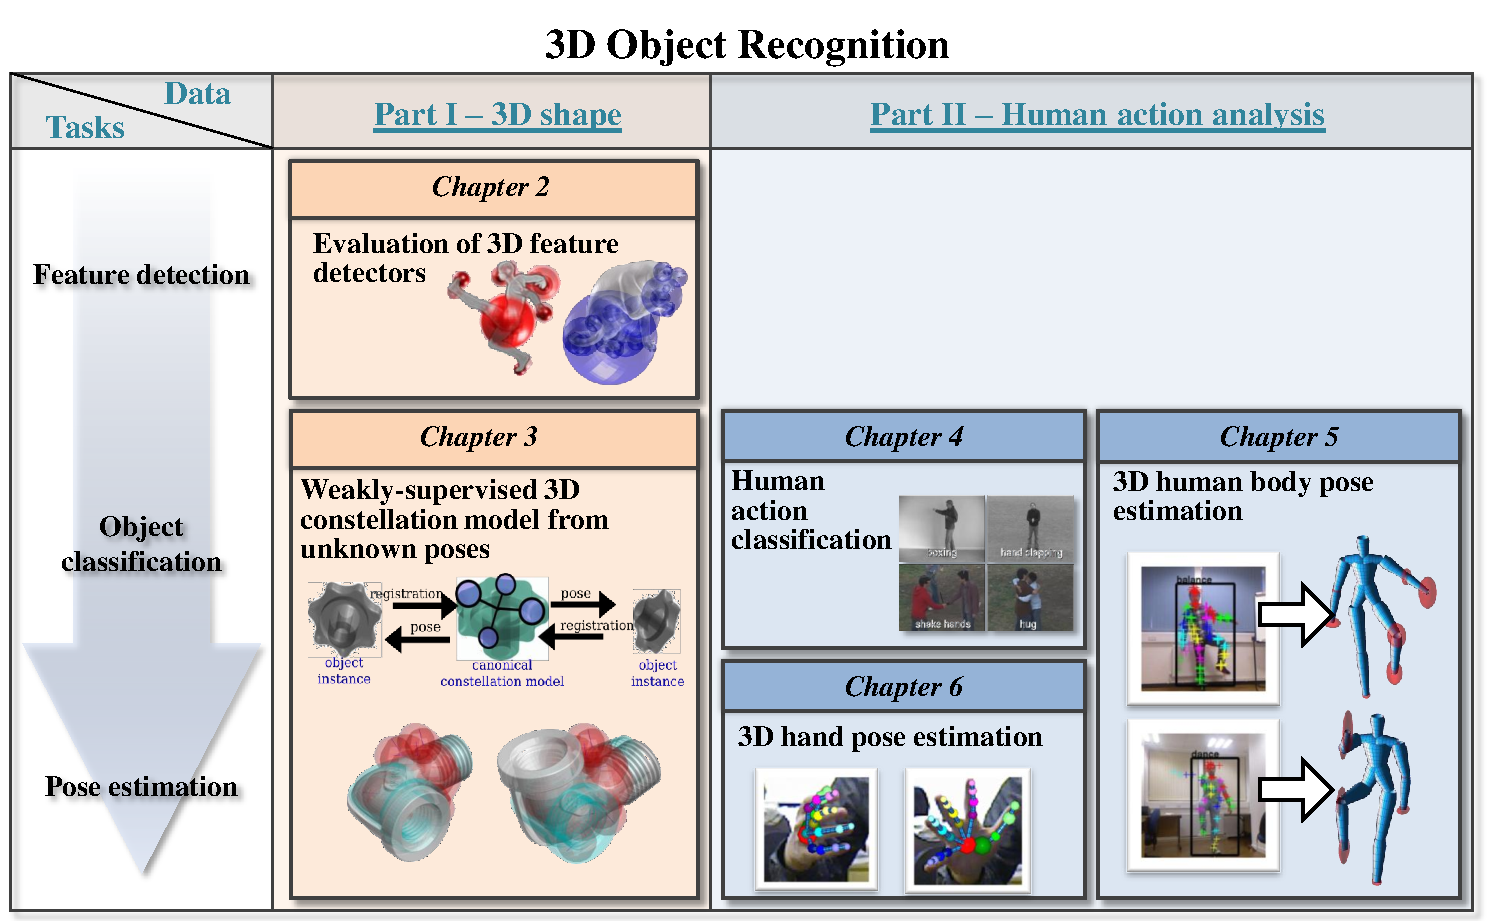
\includegraphics[width=1\linewidth]{./fig/intro/intro.pdf}
\caption{\textbf{Thesis outline}} 
\label{fig/intro/outline}
\end{figure}

\section{Thesis overview}

\subsection{Contributions}

The main contributions of this thesis are:
\begin{itemize}
	\item A detailed performance evaluation on several state-of-the-art 3D interest point detectors.
	\item A new weakly-supervised constellation model for simultaneous 3D shape recognition and registration, using training data with unknown pose. 
	\item A real-time algorithm that combines appearance and structural information for video-based action classification using semantic texton forest. 
	\item A new technique to estimate 3D human body poses using action detection and regression random forests. 
	\item A semi-supervised 3D hand pose estimation system that combines synthetic and realistic training data. 
\end{itemize}

\subsection{Limiting the scope}

% Some thing which is not considered?
In order to concentrate on the most important and relevant topics, 
several applications are not considered within this thesis. 
The first is recognition of 3D meshes \cite{Zaharescu2009, Bronstein2011, Kokkinos2012}. Textured mesh is a standard representation of 3D shapes in computer graphics and computer-aided design (CAD) tasks. However, realistic 3D shape data are usually captured in textureless point clouds, depth images or voxels. In addition, instances of the same object class can have very different textures, texture-based features are therefore not suitable for shape classification.      

The second application is model-based 3D object recognition, \eg \cite{Mian2006, Rothganger2006, Shang2010}. A pose estimator is trained on different objects in a specific scene, rather than object instances from the same class. The performances of object recognition and pose estimation of such approach rely mainly on feature matching between the model and query object instance. 

Thirdly, marker-based motion capture systems are not included in the scope of this thesis. They have been widely employed in computer-generated imagery for films and games. Markers are localised accurately from a calibrated camera system, using simple computer vision techniques. Poses are estimated straightforwardly by mapping the markers to a predefined articulated skeleton.
 With a calibrated camera network, 3D human poses can be recovered using marker-based approaches easily.  

Finally, body shape estimation from images and videos are not considered in the thesis \cite{Guan2009, Rother2009, Chen2011}. It reconstructs 3D human shapes directly from testing data, instead of parameterised poses of a articulated model. Body pose estimation is concerned with understanding the semantics of the subject and the scene, rather than reconstructing them accurately. 

\subsection{Outline}

This thesis is outlined in figure \ref{fig/intro/outline}. In the first part, chapter \ref{chap/eval} and chapter \ref{chap/reg} focus on the recognition and pose estimation of 3D shapes; the second part, chapter \ref{chap/act} -- \ref{chap/hand}, focuses on human action analysis, including action categorisation and 3D pose estimation of human body and hand gestures. Chapter \ref{chap/conclusion} concludes the thesis with possible directions for future research. 

\subsection*{Part I --- 3D Shape}

%\paragraph{Chapter 2.} This chapter presents a literature review of 3D shape processing techniques.  Recent topics about 3D feature detection, shape representation, shape recognition and pose estimation are discussed.  

\subsubsection*{Chapter 2. Evaluation of 3D feature detectors} 
A performance evaluation of volumetric 3D interest points is presented in this chapter. 
It first gives a brief introduction to the volumetric interest point detectors used in existing literature.
There interest point detectors are evaluated quantitatively using a new performance metric.
Finally, qualitative characteristics of the candidate detectors are also discussed in this chapter. 

\subsubsection*{Chapter 3. 3D Constellation model from unknown pose}
This chapter presents a weakly supervised constellation model for simultaneous 3D shape recognition and pose estimation. 
The proposed model learns the shape, appearance and pose of an object class from training exemplars, \eg images or point clouds, which contain examples of the object in unknown poses.  

\subsection*{Part II --- Human action analysis}

%\paragraph{Chapter 5.} This chapter introduces various sub-problems in human action analysis, including human action recognition, body pose estimation and hand pose estimation.  It discusses the application of random forests and its variants to model human actions and poses. It also reviews the existing approaches for the above sub-problems. 

\subsubsection*{Chapter 4. Human action classification} 
This chapter addresses the recognition sub-problem in human action analysis. A spatiotemporal semantic and structural forest is proposed to recognise human actions in real-time.    

\subsubsection*{Chapter 5. 3D human body pose estimation} 
This chapter presents a new approach to 3D body pose estimation in unconstrained, monocular videos. 
A new hybrid decision forest is introduced, in order to perform action detection and pose estimation simultaneously. 
Pose estimation is based on action detection, which includes joint classification and localisation of actions in videos. 
% By combining regression random forests with action detection, the proposed method infers 3D poses from unconstrained, monocular videos. 

\subsubsection*{Chapter 6. 3D hand pose estimation} 
This chapter addresses the sub-problem of 3D hand pose estimation. 
The regression tree learning algorithm introduced in chapter \ref{chap/body} is further developed to estimate 3D hand pose from different viewpoints. 
A data-driven inverse kinematic scheme is also described to refine the occluded joints.

\label{part/shape}
\part{3D Shape}
\chapter{Evaluation of 3D feature detectors}
\label{chap/eval}

\section{Introduction}

\begin{figure}[t]
	\centering 
	\begin{subfigure}[t]{0.30\linewidth} 
		\centering 
		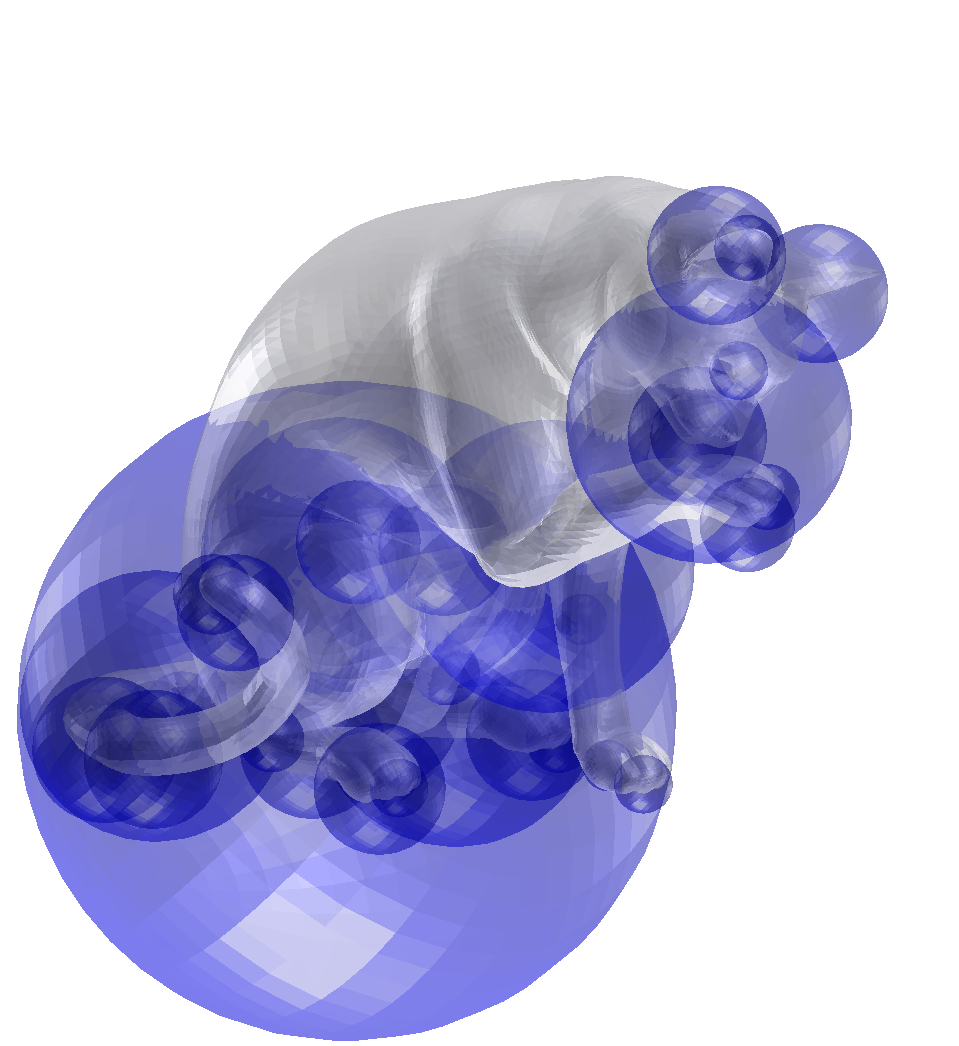
\includegraphics[width=1\linewidth]{./fig/eval/cat_dog.png} 
		\subcaption{DoG}
		\label{fig/eval/testshapes/dog}
	\end{subfigure}
	\begin{subfigure}[t]{0.30\linewidth} 
		\centering 
		\raisebox{-7mm}{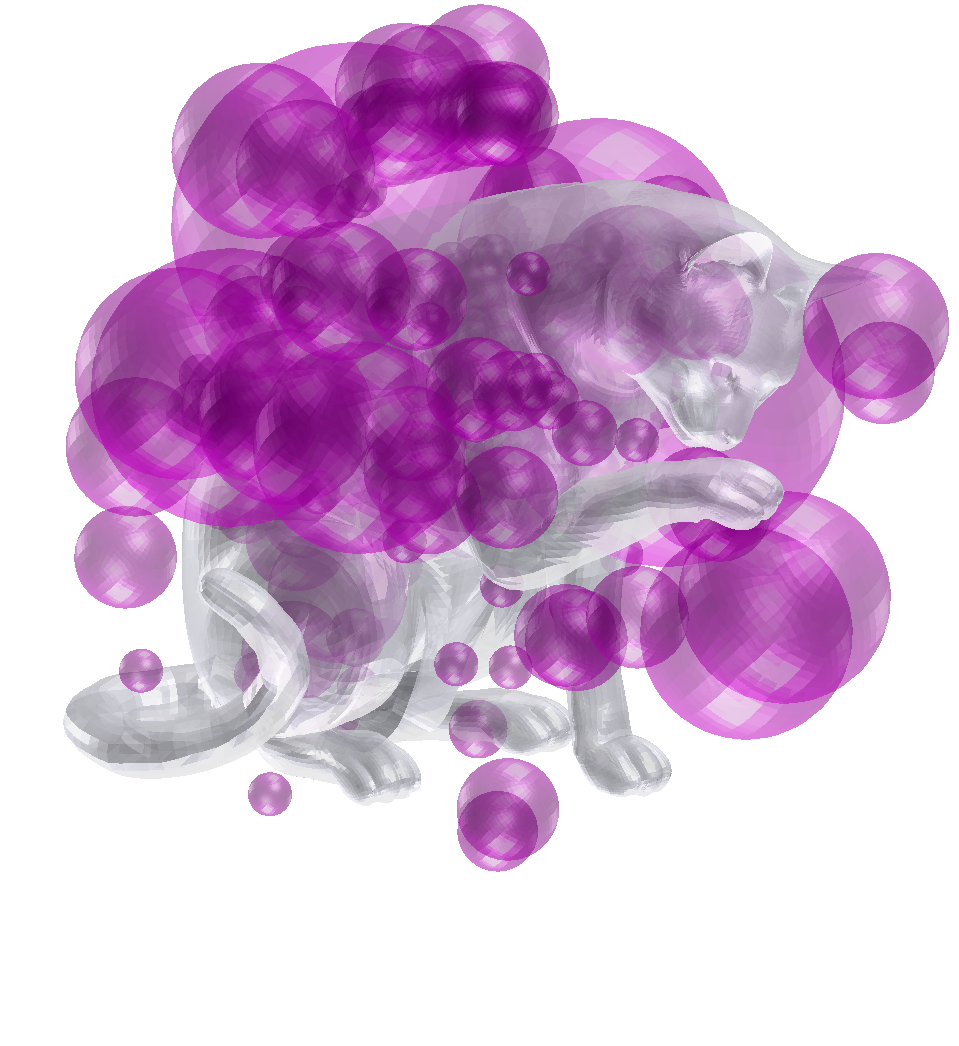
\includegraphics[width=1\linewidth]{./fig/eval/cat_surf.png}}
		\vspace{-7mm}
		\subcaption{SURF}
		\label{fig/eval/testshapes/surf}
	\end{subfigure}
	\begin{subfigure}[t]{0.30\linewidth} 
		\centering 
		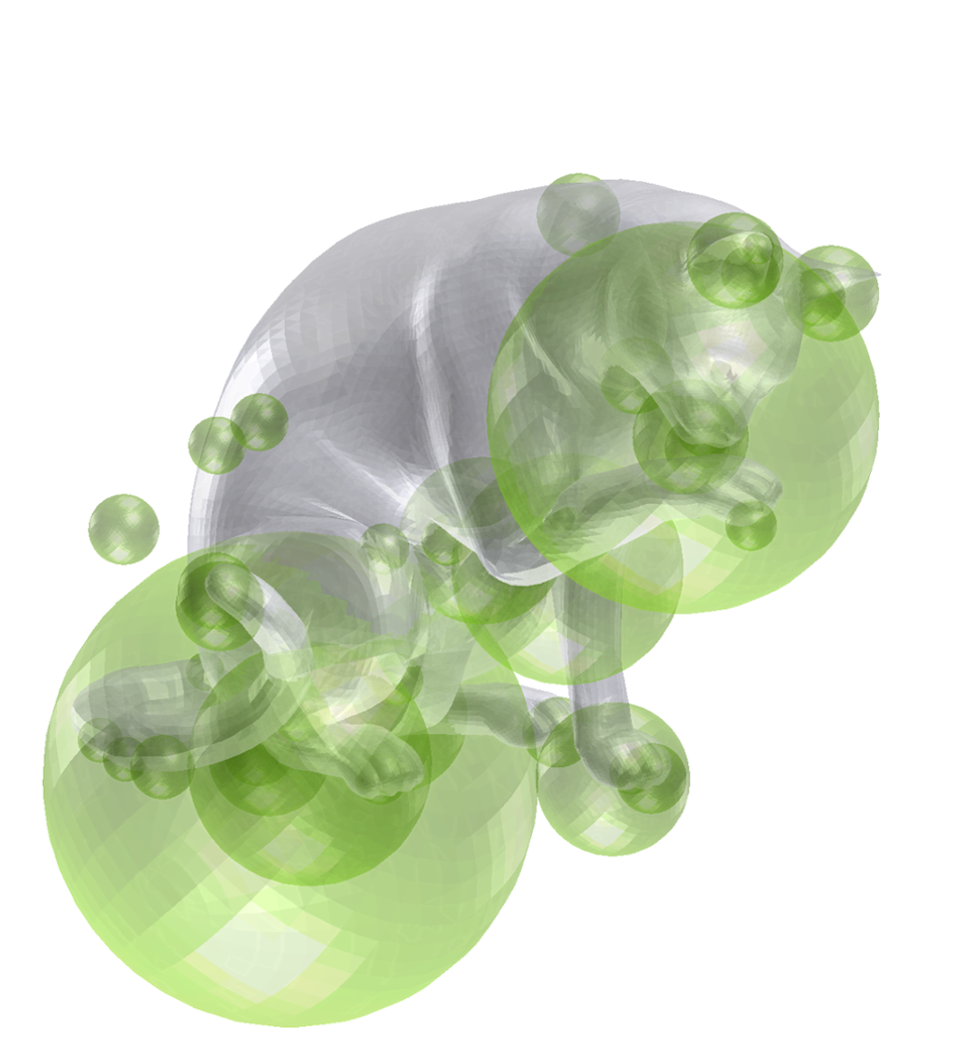
\includegraphics[width=1\linewidth]{./fig/eval/cat_harris.png} 
		\subcaption{Harris}
		\label{fig/eval/testshapes/harris}
	\end{subfigure} \\ 
	\begin{subfigure}[t]{0.30\linewidth} 
		\centering 
		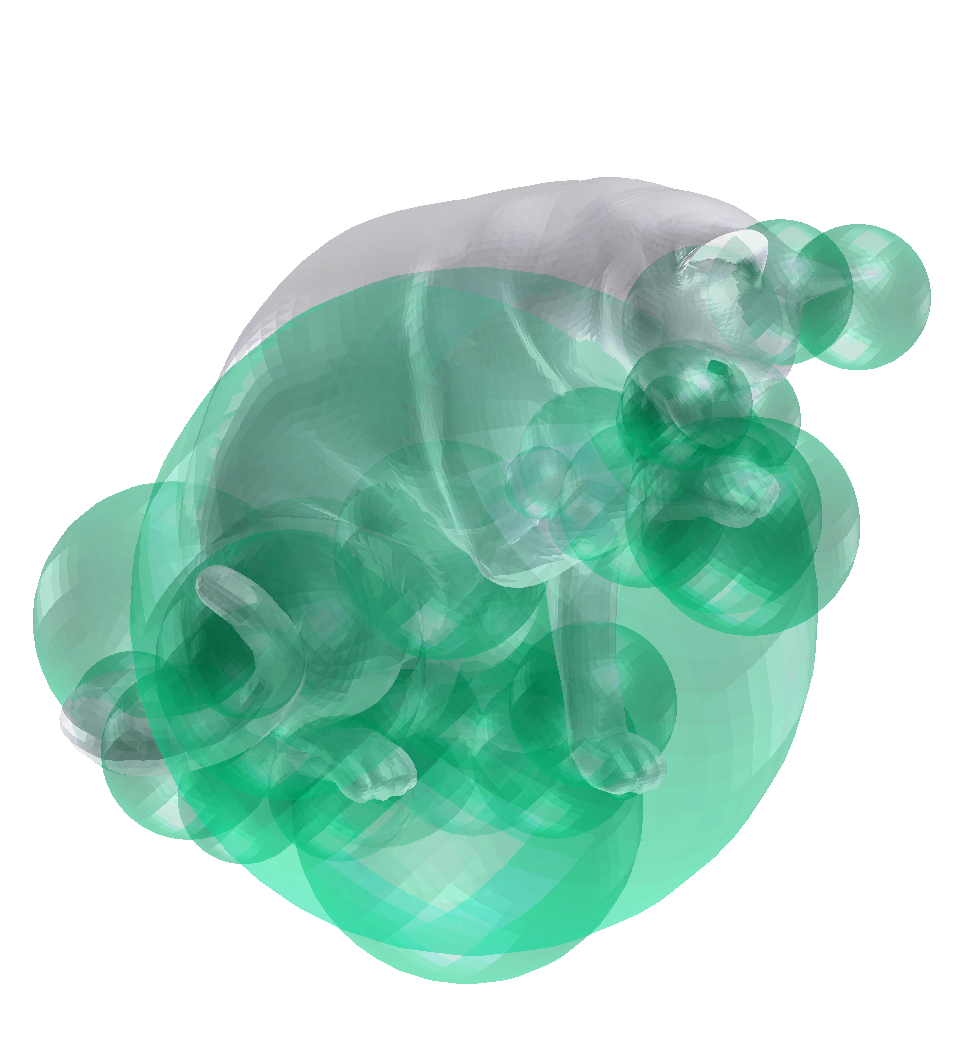
\includegraphics[width=1\linewidth]{./fig/eval/cat_hessian.png} 
		\subcaption{Hessian}
		\label{fig/eval/testshapes/hessian}
	\end{subfigure}
	\begin{subfigure}[t]{0.30\linewidth} 
		\centering 
		\raisebox{-5mm}{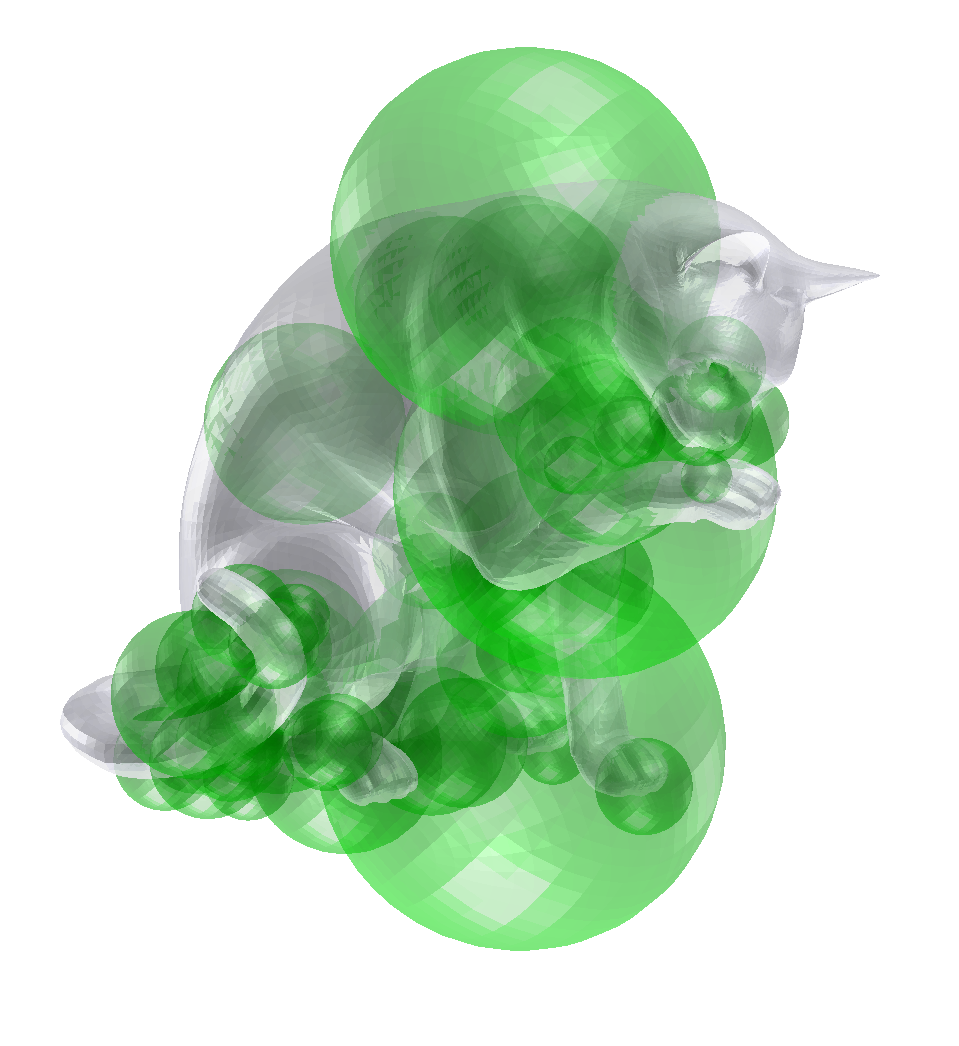
\includegraphics[width=1\linewidth]{./fig/eval/cat_fast.png}}
		\vspace{-5mm} 
		\subcaption{VFAST}
		\label{fig/eval/testshapes/fast}
	\end{subfigure}
	\begin{subfigure}[t]{0.30\linewidth} 
		\centering 
		\raisebox{-3mm}{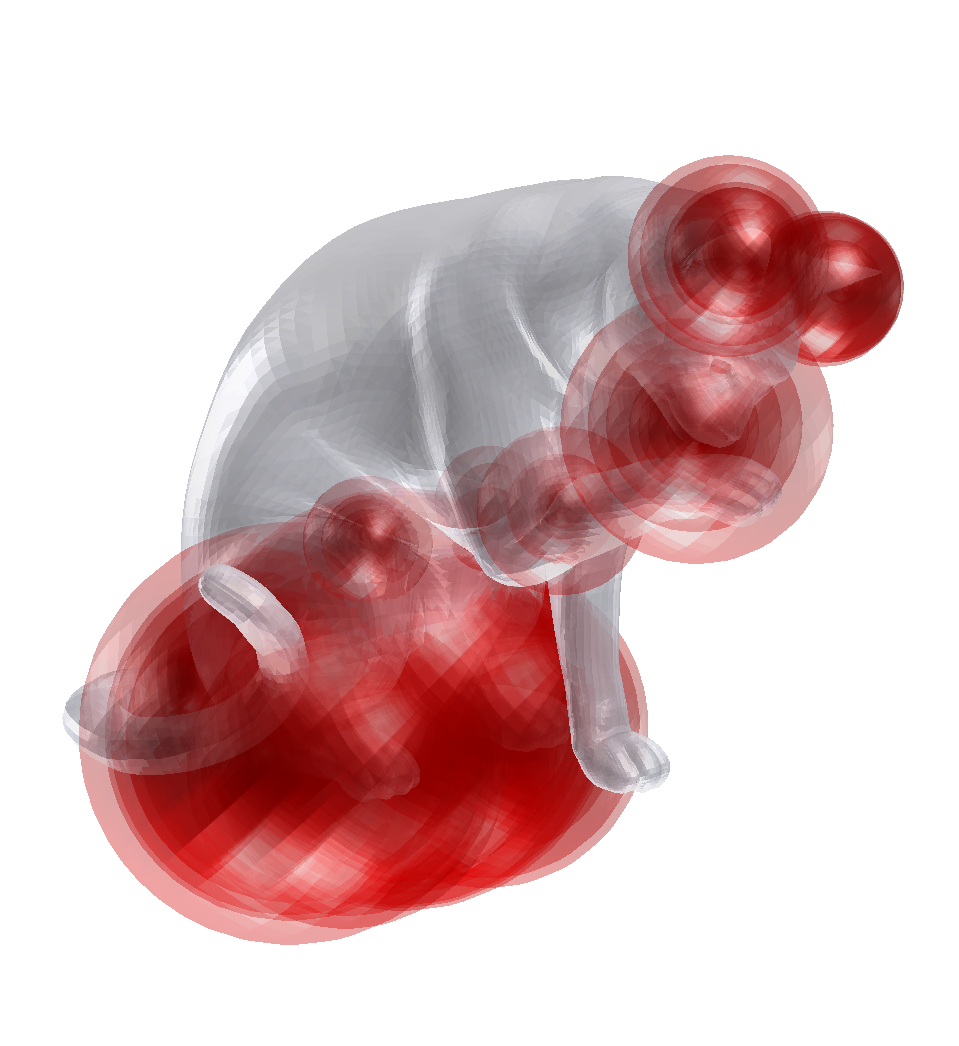
\includegraphics[width=1\linewidth]{./fig/eval/cat_mser.png}}
		\vspace{-5mm}	
		\subcaption{MSER}
		\label{fig/eval/testshapes/mser}
	\end{subfigure}
	\caption{\label{fig/eval/testshapes}Different volumetric interest points detected on a test 3D shape.}
\end{figure}

% This paragraph move to introduction! 
\iffalse 
The applications of object detection, recognition and registration are of great importance in computer vision. 
Much work has been done in solving these problems using appearance on 2D images, helped by the advent of image descriptors such as SIFT and learning-based classifiers such as SVM, and these methods are now reaching maturity. 
However, advancing geometry capture techniques, in the form of stereo, structured light, structure-from-motion and sensor technologies such as laser scanners, time-of-flight cameras, MRIs and CAT scans, pave the way for the use of shape in these tasks, either on its own or complementing appearance. Whilst an object's appearance is a function not only of its texture, but also its pose and lighting, an object's 3D shape is invariant to all these factors, providing robustness as well as additional discriminative power.
\fi  

% done 
Recognition of 3D data is not a new topic in computer vision, \eg \cite{Fisher1987, Nevatia1977, Marr1978, Bolles1983}, though such applications have seen a recent resurgence. Approaches to 3D object recognition range from the local to the global. 

% done 
At the global end are those which form a descriptor from an entire object. Such methods generally offer excellent discrimination plus robustness to shape variation, but, since the whole object is required and its extent known, they do not cope well with clutter or occlusion. Also, albeit suitable for recognition, many of the matching algorithms do not consider object pose for registration. 

% done 
At the other end of the spectrum are highly local features, such as points. Being completely non-discriminant, such features are usually embedded in a framework that finds geometrical consistency of features across shapes, \eg iterative closest point (ICP) \cite{Besl1992} and RANSAC \cite{Brown2005, Papazov2011}. 
These geometrical consistency frameworks make matching among 3D instances costly, but they also provide pose for object registration, and the local nature of features provides robustness to clutter and partial occlusion. 

%Between these two extremes are those methods that describe local features of limited but sufficiently distinctive scope, 
However, most existing methods are positioned between the two extremes, where local features describe a limited but sufficiently distinctive scope, thereby leveraging the discriminability of global methods and the robustness of local methods. 
Such features can be used for effective object detection, recognition and registration. The nature of these hybrid methods is reminiscent of the image descriptors of appearance-based methods, not least in the need for shape features to be chosen at points that are repeatably locatable in different datasets, and whose localities are distinctive. 
A common and crucial stage of such approaches is therefore the detection of interest points to be described.  

% done 
This chapter is concerned with a performance evaluation of interest point detectors on scalar volumetric data, as shown in figure \ref{fig/eval/testshapes}.   
As discussed in chapter \ref{chap/intro}, different from other data-specific 3D interest point detectors for meshes \cite{Sipiran2011,Glomb2009,Zaharescu2009} or point-clouds \cite{Aanaes2012,Unnikrishnan2008}, feature detection from scalar volumetric data is more versatile. Such data not only comes directly from volumetric sensors, such as MRIs, but can also be generated or converted from other three dimensional data representations, such as point clouds, meshes or depth maps, making the proposed evaluation experiments widely applicable to various applications.
In addition, visual saliency of volumetric interest points is defined in a scalar volume but not on a local surface patch. This full three dimensional representation implies that interest points can be located off an object's surface, \eg inside a cavity or voxels with varying intensities. 
Furthermore, voxels, which is the 3D equivalent of pixels, make repurposing the many 2D interest point detectors for 3D straightforward. 

% done 
The primary quantitative evaluation criterion used in this work is a novel measure combining both repeatability, based on the number of corresponding points found across two volumes, and the spatial accuracy of correspondences. Detected interest points have a (subvoxel) location and a scale, and distances are computed in this space. The qualitative characteristics of the candidate volumetric interest points are also presented. 

% no need 
\iffalse 
The following section reviews previous work relevant to interest point detectors and our evaluation framework. Section \ref{sec/eval/detectors} introduces the interest point detectors used in the evaluation experiments, while section \ref{sec/eval/methodology} explains the proposed evaluation methodology.   
Section \ref{sec/eval/experiments} presents the evaluation experiments and their corresponding quantitative and qualitative analyses, before we conclude in section \ref{sec/eval/conclusion}.
\fi 

%-------------------------------------------------------------------------
\section{Related work}
\label{sec/eval/relatedwork}

\subsection{Interest point detectors}

%  done 
The process of interest point detection is the first stage of many object recognition tasks, including object classification and pose estimation. An interest point detector localises salient features from input visual data for further processing. The detected interest points are typically used to match corresponding points across two or more similar sets of data. 
The majority of earlier studies focus on detecting features on 2D images. The paradigm of 2D interest point detection has already been well studied, for instance Tuytelaars and Mikolajczyk \cite{Tuytelaars2008} performed an extensive survey on locally-invariant feature detectors.  

% done 
Recent advancements in data acquisition techniques have greatly improved the availability of 3D shape data. Large scale synthetic and realistic 3D repositories, such as Google Warehouse \cite{Lai2010} and the B3DO dataset \cite{Janoch2011}, have attracted much interest in 3D shape-based object recognition applications. Consequently, various 3D interest point detection techniques have been proposed alongside with this emerging field of computer vision research. 

% done 
Existing techniques for 3D interest point detection are categorised as volume-based or geometry-based detectors, according to the representation of input data. Volume-based detectors operate directly on the pixel/voxel values of volumetric scalar data. This type of data includes CT scan volumes \cite{Flitton2010}, binary volumes generated from depth images \cite{Viksten2008} or 3D meshes \cite{Knopp2010}, and time-varying video data \cite{Koelstra2009, Laptev2005, Willems2008, Yu2010}. 
Geometry-based interest point detectors locate interest points by exxtracting geometric information, such as contours, surface normals and surface patches. 
Common data representations of geometry-based techniques include synthetic meshes \cite{Glomb2009,Sipiran2011,Zaharescu2009} or point clouds \cite{Unnikrishnan2008,Aanaes2012}. 
Literature reviews of this category of interest point detectors were reported by Salti \etal \cite{Salti2011} and Dutagaci \etal \cite{Dutagaci2011}.  
Nevertheless, unlike 2D interest points, performance evaluation of 3D interest points remains an unexplored topic. 
Hence, this chapter performs the quantitative and qualitative evaluation of volumetric interest point detectors, whose high versatility with respect to original data representation enable a wider coverage of potential applications.

% The remainder of this section will review the interest point detectors used in our evaluation, which we divide into two classes based on their definitions of local features.

% done 
\subsubsection{Corner detection}
The first class of interest point detectors aim to find corners from the input data.
The Harris interest point detector \cite{Harris1988} is a classic image-based corner detection algorithm, which finds points of large gradient changes in orthogonal directions. It detects interest points by analyzing the eigenvalues of the second moment matrix (first order derivative). Its 3D adaptations have been applied to registration of volumetric CT scans \cite{Ruiz-Alzola2001, Dalvi2010}.  
Building on the success of Harris corner detector, Mikolajczyk \cite{Mikolajczyk2004} developed the scale-covariant Harris-Laplace detector by finding Harris corners in the spatial domain which are maxima of the Laplacian in the scale domain. 
This approach was extended to space-time interest points for video classification by Laptev \cite{Laptev2005}. 

Instead of detecting corners by image gradients, corner detectors that operate directly on image pixels were also proposed. 
Smith and Brady \cite{Smith1997} presented SUSAN corner detector. It leveraged the proportion of pixels in a neighbourhood, which were dissimilar to the central pixel value.
The FAST corner detector by Rosten \etal \cite{Rosten2010} used the accelerated segment test (AST), a relaxed version of SUSAN, to locate stable corners in an image.  
FAST measures the largest number of contiguous pixels on a circle which are significantly darker, or brighter, than the centre pixel. Without computing the derivative at each pixel, the speed of FAST can be further improved by learning a decision tree classifier for feature detection. Due to its efficient run-time performance, several volumetric feature detectors have been applied to space-time volumes classification based on FAST interest points \cite{Koelstra2009,Yu2010}. 

\subsubsection{Blob detection}

% done 
Lindeberg \cite{Lindeberg1998} studied scale-covariant interest points using the Laplacian-of-Gaussian kernel, which is mathematically equivalent to the trace of the Hessian, as well as the determinant of the Hessian (DoH). Lowe \cite{Lowe2004} approximated the above LoG kernel by a Difference-of-Gaussians (DoG) operator for better computational performance. Recently, the DoG approach was applied to 3D object detection and recognition of synthetic meshes \cite{Wessel2006}, volumetric scans \cite{Flitton2010} and multi-view stereo data \cite{Pham2011}.

% done 
The Hessian-Laplace detector, by Mikolajczyk and Cordelia \cite{Mikolajczyk2004}, is similar to Harris-Laplace detector. Interest points are detected by evaluating the Hessian matrix of an input image. Similarly, Bay \etal \cite{Bay2008} proposed the speeded-up robust feature (SURF), which accelerated the computation time of determinant-of-Hessian operator using integral images and box filters. Since then SURF has been applied to videos \cite{Willems2008} and volumetric data generated from synthetic 3D mesh models \cite{Knopp2010}.

% done 
Region-based detector relies on finding salient regions instead of interest points, an example is maximally stable extremal region (MSER) proposed by Matas \etal \cite{Matas2004}. 
While both DoG and SURF are grounded on the approximation of the Laplacian-of-Gaussian kernel, MSER finds thresholded regions whose areas are maximally stable as the threshold changes. 
Hence, MSER is inherently multi-scale, as well as invariant to affine intensity variations and covariant with affine transformations. Three dimensional MSER has already been applied to volumetric data, firstly in the context of segmentation of MRIs \cite{Donoser2006}, and then on video data \cite{Riemenschneider2009}.

\subsubsection{Covariant characteristics}

% done
A feature characteristic is considered covariant when it undergoes the same transformation as the data. 
Image-based detectors have been made affine-covariant, in order to approximate the perspective distortion caused by projection of 3D world onto the 2D image plane \cite{Mikolajczyk2002}. 
Such covariance is not necessary with 3D shapes because most shape acquisition techniques do not have the 3D-2D projection process, thus invariant to view point changes. 
However, objects might have varying poses during data acquisition, such as translation, rotation and scaling for rigid shapes. Rotation and scale covariance are therefore still essential requirements for processing 3D shape data. 
In addition, 3D shape data are generally not affected by illumination and lighting conditions, except for texture-mapped meshes \cite{Zaharescu2009}, the quality of shape data is instead determined by the amount of noise and sampling artifacts, \eg holes and occlusions, of the reconstruction process. 

\subsection{Methodologies}

% done 
Empirical performance evaluation is a popular topic in computer vision, and the evaluation of interest point detectors is no exception. Different approaches of performance evaluations can be categorised according to the evaluation criteria and the source of ground truth interest point locations. 

\subsubsection{Evaluation criteria}

Some methods evaluate performance in the context of a particular task, \eg object recognition \cite{Shin1999, Dutagaci2011}. Such evaluations can be carried out conveniently with a target detector and a groundtruth dataset, but they also lack generality to other applications. 

Most evaluation frameworks investigate one or more interest point characteristics. 
One such characteristic, important for registration applications, \eg camera calibration, scene reconstruction and object registration, is the accuracy of interest point localisation. 
Coelho \etal \cite{Coelho1992} measured localisation accuracy by computing projective invariants and comparing these with the actual values measured from the scene. 
Brand and Mohr \cite{Brand1994} introduced three further measures, including 2D Euclidean distance from detected points to ground truth corner locations, given by line fitting to a grid. This approach was extended to using the distance to the nearest point detected in, and transformed from, another image by Schmid \etal \cite{Schmid2000}. 
Laptev \cite{Laptev2003} matched interest points found over location and scale, 
Matching scores for interest points found over location and scale \cite{Laptev2003}. Furthermore, Mikolajczyk \etal \cite{Mikolajczyk2004} used affine transformations to evaluate interest point pairs. 

% done 
For object recognition, two other important characteristics of interest points are their repeatability and distinctiveness. 
Repeatability considers the geometrical stability of the corresponding interest points among multiple input data taken under varying conditions. 
It was proposed and defined by Schmid \etal \cite{Schmid2000} as the ratio of repeated points to detected points. Schmid \etal \cite{Schmid2000} also introduced entropy, or information content, as a quantitative measure of distinctiveness.
In order to compensate for the effect of the detectors' sensitivity, Rosten \etal \cite{Rosten2010} used the area under the repeatability curve as a function of number of interest points, varied using a threshold on the detector response, in their evaluation. 
When ground truth locations of interest points are given, \eg a pair of hand-laballed images, an alternative measure is the ROC curve, which considers interest point matching as a binary classification process \cite{Bowyer1999}. Alternatively, qualitative visual comparisons are also used alongside quantitative analyses, on test datasets containing a variety of different interest points \cite{Lindeberg1998, Laptev2005}. Data for qualitative evaluation are often selected to investigate the characteristics of interest points under certain challenging conditions, such as changing camera pose, sampling noise and compression artifacts. 

% done 
In the context of image-based interest points, performance of detectors are often measured over variations in image rotation, scale, viewpoint angle, illumination and noise level, \eg \cite{Schmid2000} covers all these factors, as well as corner properties \cite{Rajan1989}. Efficiency is also a further consideration for applications, of which run-time performance is a major concern \cite{Rosten2010}, such as an object recognition system on mobile phone. Nevertheless, evaluations of 3D interest points not only vary on the above-mentioned criteria, but also on the type of data, such as meshes, space-time volumes, point clouds and space volumes.

% done 
% It is also worth noting that the distinction between interest point detectors and descriptors. The latter topic, also well evaluated in 2D, \eg \cite{Mikolajczyk2005}, has a concept of both correct and incorrect matches, allowing the use of recall-precision as an evaluation criterion.

% done 
\subsubsection{Ground truth data} 

%With both localisation accuracy and repeatability criteria, the ground truth location of interest points in the scene must be known. The ground truth data can be computed in a variety of ways. 
In order to compute any of the aforementioned interest point characteristics, the groundtruth locations of interest points, or alternatively the groundtruth homography between two evaluation instances, must be known. Groundtruth information can be obatined in a varity of ways.  
Several approaches specify the location of interest points in an image, either known by design \cite{Rajan1989}, or hand-labelled by multiple people \cite{Heath1997}. 
Other methods find corresponding pairs of point across two or more images. For example, matching is achieved using planar scenes and computing homographies between images \cite{Schmid2000}, scenes of known geometry manually registered in each image \cite{Rosten2010}, scene geometry captured using structured light \cite{Aanaes2012}, and synthetic data \cite{Laptev2005}. 
In addition, ground truth data for 3D interest point evaluations are likewise obtained from manual annotation \cite{Dutagaci2011}, known projection homography of stereo point clouds \cite{Aanaes2012} and synthetic shape data \cite{Salti2011}. 

% done 
\section{Detectors}
\label{sec/eval/detectors}

Generally every new volumetric interest point was proposed with an applications in mind, such as shape retrieval and classification \cite{Riemenschneider2009,Flitton2010,Knopp2010,Prasad2011}, medical imaging \cite{Criminisi2011,Ni2008,Donner2011} and video classification \cite{Willems2009,Laptev2005,Yu2010}. 
Whilst interest point detectors for images have already been studied extensively \cite{Mikolajczyk2005, Tuytelaars2008}, evaluation of 3D interest points remains largely unexplored. 

This section describes the principles and formulations of the 3D interest points evaluated in the experiments. These include DoG \cite{Flitton2010, Pham2011}, DoH and Harris-based interest points \cite{Laptev2005}, SURF \cite{Willems2008, Knopp2010}, VFAST \cite{Yu2010} and MSER \cite{Donoser2006, Riemenschneider2009}. 

\subsection{Scale-space and subpixel-refinement}
\label{sec/eval/subvoxel}

% done 
Scale covariance of interest points is achieved by creating a scale-space of the input volumetric data. An octave of linear scale-space is created by convolving the input volume with a Gaussian smoothing kernel. Such smoothing kernel is applied on the volume recursively to suppress fine-scale structures. Afterwards a new octave is created by down-sampling the input volumes from the previous octave. As a result, a series of volumes, with multiple levels of details, is created. The detailed implementation of scale-space, with respect to interest point detection, can be found in \cite{Lindeberg1998}. 

% done 
However, scale-space representation is not computed for MSER because it detects salient regions in different scales. MSER locates interest points by fitting an ellipsoid to the detected salient region \cite{Matas2004}. For other interest point detectors, saliency responses are computed in all volumes within the scale-space. In addition, the subpixel refinement process of \cite{Lowe2004} is applied on these detectors. Interest points are localised at the subvoxel level by fitting 4D quadratic functions around the local scale-space maxima, and selecting the maxima of those functions instead. 

% done 
\subsection{Difference-of-Gaussians (DoG)}
The DoG operator is a blob detection technique for feature localisation popularised by the SIFT algorithm \cite{Lowe2004}. DoG approximates the Laplacian-of-Gaussian filter, which detects features of a particular size. 
The saliency response of DoG detector $S_{\textrm{DoG}}$ is computed by subtracting two Gaussian smoothed volumes, usually adjacent scale-space representations, of the same input data and taking the absolute values of the difference.
Interest point are detected at the 4D local maxima, \ie 3D space plus scale, by the saliency response $S_{\textrm{DoG}}$ within each octave of $\mathbf{v}(\mathbf{x},\sigma_s)$ in equation \ref{eqn/eval/dog}.
\begin{equation}
	\label{eqn/eval/dog} 
	S_{\textrm{DoG}}(x,y,z;\sigma_s) = |V(x,y,z;\sigma_s) - V(x,y,z;\sigma_{s-1})|
\end{equation}
Volume $V(x,y,z;\sigma_s)$ denotes the scale-space representation of the input volumetric data at scale $\sigma_s$.

\subsection{Harris}
Harris corner detector examines image gradients by shifting in a local window, interest points are detected at positions where large changes are observed in all directions \cite{Harris1988}. While the first 3D extension of the original Harris corner detector uses separate scale parameters for the heterogeneous space and time axes \cite{Laptev2005}, in this work only one scale $\sigma_s$ is shared among three homogeneous spatial axes for simplicity.  
The second-moment matrix $\mathbf{M}$ is computed by smoothing the first derivatives of the volume in scale-space $\mathbf{v}(\mathbf{x};\sigma_s)$ by a spherical Gaussian weight function $g(\cdot;\sigma_\textrm{Harris})$:  
\begin{equation}
	\begin{aligned}
		\mathbf{v}_x(\mathbf{x};\sigma^2_s) &= \displaystyle\frac{\partial \mathbf{v}(\mathbf{x};\sigma^2_s)}{\partial x} \\
		\mathbf{v}_y(\mathbf{x};\sigma^2_s) &= \displaystyle\frac{\partial \mathbf{v}(\mathbf{x};\sigma^2_s)}{\partial y} \\
		\mathbf{v}_z(\mathbf{x};\sigma^2_s) &= \displaystyle\frac{\partial \mathbf{v}(\mathbf{x};\sigma^2_s)}{\partial z} \\ 
		\mathbf{M}(\cdot, \sigma_\textrm{Harris}, \sigma_s) & = g(\cdot;\sigma_\textrm{Harris}) \ast \left[
			\begin{array}{ccc}
				\mathbf{v}^2_x & \mathbf{v}_x\mathbf{v}_y & \mathbf{v}_x\mathbf{v}_z \\
				\mathbf{v}_x\mathbf{v}_y & \mathbf{v}_y^2 & \mathbf{v}_y\mathbf{v}_z \\
				\mathbf{v}_x\mathbf{v}_z & \mathbf{v}_y\mathbf{v}_z & \mathbf{v}^2_z \\
			\end{array}
		\right]
	\end{aligned}
	\label{eqn/eval/harris_2ndmoment}
\end{equation}
where $\mathbf{v}_x$,$\mathbf{v}_y$,$\mathbf{v}_z$ denote the partial derivatives of the volume in scale-space $\mathbf{v}(\mathbf{x};\sigma_s)$ along $x$, $y$ and $z$ axes respectively. The second moment matrix $\mathbf{M}$ describes the autocorrelation along different directions in a local neighbourhood of size $\sigma_s$. 

Candidate interest points are located at coordinates $(x,y,z)$ where the second-moment matrix $\mathbf{M}(x,y,z; \sigma_\textrm{Harris}, \sigma_s)$ has large eigenvalues $\lambda_1, \lambda_2, \lambda_3$. Interest point are hence the 4D local maxima in the scale-space of $S_{\textrm{Harris}}$. Locations of interest points are refined using the sub-voxel refinement method described in \ref{sec/eval/subvoxel}. The window size $\sigma_\textrm{Harris}$ is proportional to expected feature scales $\sigma_s$ by a factor of $0.7$ as suggested in \cite{Mikolajczyk2004}. 

The saliency response of Harris corner, $S_\textrm{Harris}$, is computed from the determinant and trace of $\mathbf{M}$: 
\begin{equation}
	S_\textrm{Harris} = \sigma_{s}^3 \:\det(\mathbf{M}) - \kappa\:\mathrm{Tr(\mathbf{M})}^3
	\label{eq/eval/harriscorner}
\end{equation}
where $\kappa$ is a tunable sensitivity parameter that controls the reject of edge points.  
Saliency response $S_\textrm{Harris}$ is normalised by its scale $\sigma_s$ as shown in equation \ref{eq/eval/harriscorner}.

% done 
\subsection{Determinant-of-Hessian (DoH)}
\label{sec/eval/doh}
The DoH interest point is similar to the Harris detector with respect to formulation \cite{Lindeberg1998}. Instead of computing the second-moment matrix $\mathbf{M}$, a Hessian matrix $\mathbf{H}$ is computed: 
\begin{equation}
	\mathbf{H} = 
	\left[
		\begin{array}{ccc}
			\mathbf{v}_{xx} & \mathbf{v}_{xy} & \mathbf{v}_{xz} \\
			\mathbf{v}_{yx} & \mathbf{v}_{yy} & \mathbf{v}_{yz} \\
			\mathbf{v}_{zx} & \mathbf{v}_{zy} & \mathbf{v}_{zz} 
		\end{array}
	\right]
	\label{eqn/eval/hessianmatrix}
\end{equation}
where $\mathbf{v}_{xy}$ denotes the second derivative of the volume at scale $\sigma_s$, along $x$ and $y$ axes, such that
\begin{equation}
	\mathbf{v}_{xy} = \frac{\partial \mathbf{v}(\mathbf{x};\sigma_s)}{\partial x \partial y}
	\label{eqn/eval/hessiandiverative}
\end{equation}
The saliency response is the scale-normalised determinant of Hessian matrix $\mathbf{H}$:
\begin{equation}
	S_{\textrm{Hessian}} = \sigma^3_s \:\mathrm{det}(\mathbf{H})
	\label{eqn/eval/hessiansaliency}
\end{equation}
Subsequently, interest points are located at the 4D scale-space local maxima of $S_\textrm{Hessian}$.

% done 
\subsection{SURF}
Speeded up robust features (SURF) is a feature extraction algorithm optimised for efficiency \cite{Bay2008}. The 3D, volumetric version of SURF was first introduced in \cite{Willems2008} for video classification. Recently, it was used in a 3D shape object recognition task \cite{Knopp2010}.

SURF is an efficient approximation of the DoH detector. Second-order derivatives of Gaussians in the DoH detector are approximated by six Haar wavelets, \ie box filters. Convolutions of the Haar wavelets can be greatly accelerated using integral videos/volumes. The saliency response of 3D SURF is similar to the aforementioned DoH detector. 

% done 
\subsection{VFAST}
\label{sec/eval/vfast}

Building on the success of the FAST corner detector \cite{Rosten2010}, VFAST \cite{Yu2010} and FAST-3D \cite{Koelstra2009} have been introduced to video-based object classification. 
The VFAST interest points are detected by directly comparing intensities in the video sequences. Similar to FAST, the VFAST detector can be further accelerated by learning a decision tree-based corner detector from training videos \cite{Rosten2010}. 

The VFAST algorithm performs accelerated segment tests (AST) on three orthogonal planes, $XY$, $XZ$ and $YZ$. The saliency score is computed by maximising the differences $\{ t_{XY}, t_{XZ}, t_{YZ} \}$ that makes at least $n$ contiguous voxels brighter or darker than the nucleus voxel $\vxpatch(x,y,z)$ by a threshold $\delta_{V}$. Consider the voxels values $\becire_{XY}$ on the $XY$ Bresenham circle $\becir_{XY}$, $AST(x,y,z)$ is computed as follows. 
\begin{align}
	t_{XY} & = \max\left(| \vxpatch(x,y,z) > \becire_{XY}|; \quad \forall \becire_{XY} \in \becir_{XY} \right)\\ 
AST_{XY}(x,y,z) & = \left\{
\begin{array}{lc}
	t_{XY} & \mbox{if $> n$ continguous } |\vxpatch(x,y,z) - \becire_{XY}| > \delta_{V} \\
	0 & \mbox{ otherwise }
\end{array}
\right. 
\label{eqn/eval/fastast}
\end{align}
where $\becire_{XY}$ denotes a voxel on an $XY$-circle centered at $\vxpatch(x,y,t)$. The combined saliency response $S_{\textrm{vfast}}$ is the Euclidean norm of saliency scores on the three planes in equation \ref{eqn/eval/fastverall}: 
\begin{equation}
S_\textrm{vfast} = \sqrt{ \left(AST_{XY}(x,y,t)\right)^2+ \left(AST_{XZ}(x,y,t)\right)^2+ \left(AST_{YZ}(x,y,t)\right)^2}
\label{eqn/eval/fastverall}
\end{equation}
Interest points are detected at the local maxima in $S_{\textrm{vfast}}$ over both translation and scale, with at least two non-zero responses in $AST_{XY}(n,t)$, $AST_{XZ}(n,t)$ and $AST_{YZ}(n,t)$. The steps of computing VFAST interest points are described in algorithm \ref{algo/eval/vfast}. 

\begin{algorithm}
\caption{VFAST interest point detector}
\label{algo/eval/vfast}
\begin{algorithmic}
	\REQUIRE $[x,y,z] = $ voxel coordinates
	\REQUIRE $r_{XY},r_{XZ},r_{YZ} = $ radii of Bresenham circles
	\REQUIRE $n = $ contiguous threshold
	\REQUIRE $\delta_{V} = $ intensity threshold
	\STATE $\becir_{XY},\becir_{XT},\becir_{YT}$ = Pixels of Bresenham circles
	\STATE $t_{XY} = \max\left(| \vxpatch(x,y,z) > \becire_{XY}|; \forall \becire_{XY} \in \becir_{XY} \right)$
	\STATE Compute $AST_{XY}(x,y,z)$ by equation \ref{eqn/eval/fastast}
	\STATE Compute $AST_{XZ}(x,y,z)$ accordingly 
	\STATE Compute $AST_{YZ}(x,y,z)$ accordingly 
	\STATE Compute $S_\textrm{vfast}$ by equation \ref{eqn/eval/fastverall}
	\STATE Discard pixels that has only one non-zero $AST(\cdot)$ function 
	\STATE Detect intest points at the 4D local maxima 
\end{algorithmic}
\end{algorithm}

% done 
\subsection{MSER}
The maximally stable extremal regions (MSER) detector is a region-based blob detection technique proposed by Matas \etal \cite{Matas2004}. Extremal regions are the connected components of a thresholded input data, which can be an image or a volume. Maximally stable regions are selected from a set of nested extremal regions obtained using different thresholds. The extremal regions of an input volume can be enumerated efficiently using the union-find algorithm which has a worst case of $O(N\log(\log(N)))$ \cite{Matas2004}, where $N$ is the number of pixels/voxels. Being inherently advantageous for volumetric interest point detection, \ie robust to rotation and scale changes, MSER has been applied to detection of volumetric salient regions \cite{Donoser2006,Riemenschneider2009}.

Normally an ellipsoid is fitted to each maximally stable region from the input data \cite{Matas2004}, the position and scale of MSER interest points being represented by the centres and radii of such ellipsoids respectively. In this work a sphere is fitted to the stable regions instead, making the interest points compatible with the proposed evaluation framework.

% done 
\section{Methodology}
\label{sec/eval/methodology}

The traditional repeatability ratio measures the repeatability of interest point detectors at a single, predefined accuracy, \eg \cite{Schmid2000}; it is therefore not only sensitive to the choice of matching distance threshold, but also gives little indication of the actual localisation accuracy, \ie the closeness of corresponding interest points, for correspondences, other than that they fall within the threshold. Hence, a single repeatability ratio is insufficient to describe the performance of interest point detectors for various applications with different accuracy requirements. 

On the other hand, real matching accuracy, \eg ROC curves in \cite{Bowyer1999}, requires hand crafted point-to-point groundtruth correspondences. This approach is difficult to generalise to large, realistic evaluation datasets such as point clouds from multi-view stereo systems.     

Whilst existing evaluations focused on either localisation accuracy or repeatability, a new performance score is used in this work, by combining the two performance metrics. The proposed combined score is computed based on \emph{repeatability ratio} with respect to \emph{varying accuracy} requirements. This section explains the combined score used in the experiments. 

% done 
\subsection{Localisation accuracy}
An interest point is considered as a sphere at coordinates $\{\pointx, \pointy, \pointz\}$ in a voxelised 3D space, with radius $\pointscale$ given by its scale. A vector $\onepoint$ is used to describe this interest point by combining its spatial location and scale: 
\begin{equation}
	\onepoint = \{ \pointx, \pointy, \pointz, \scalefactor\log(\pointscale)\}^\mathsf{T}
\label{eqn/eval/loc_vec}
\end{equation}
The logarithm of scale is used to remove multiplicative bias across detectors, and since spatial location and scale are not fully commensurate, a parameter $\scalefactor$ is introduced to weight the importance of scale to the distance function.

A key component of the proposed evaluation score is the distance metric for measuring the closeness of two corresponding interest points with respect to their locations and scales. In this work the Euclidean norm is used:
\begin{equation}
	D(\onepoint, \anotherpoint') = ||\onepoint - \anotherpoint'||_{2} 
	\label{eqn/eval/matchdistance}
\end{equation}
% A key component of the proposed evaluation score is the distance metric for measuring the closeness of two corresponding interest points with respect to their locations and scales. 
%An interest point $\onepoint$ is represented by a sphere at coordinates $[\pointx, \pointy, \pointz]$ with radius $\pointscale$ given by scale.   
%\begin{equation}
%D(\onepoint, \anotherpoint') = ||\onepoint - \anotherpoint'||_2
%\label{eq/eval/matchdistance}
%\end{equation}
%A key component of the proposed evaluation score is the distance metric used to measure the closeness of two corresponding interest points with respect to their locations and scales:
%\begin{equation}
%\onepoint = [\pointx,~\pointy,~\pointz,~f\log \pointscale]^\mathrm{T}
%\label{eq/eval/loc_vec}
%\end{equation}
%The log of scale is used to remove multiplicative bias across detectors, and since spatial location and scale are not fully commensurable, a parameter $f$ is introduced to balance the importance of scale to the distance function. 
where $\onepoint$ is the coordinate of an interest point found in the volume, $\volumep$, and $\anotherpoint'$ is the point $\anotherpoint$ found in another volume $\volumeq$, transformed into the coordinate frame of $\volumep$ using a known groundtruth homography. The evaluation score is based on the distance of an interest point to the nearest transformed interest point in equation \ref{eqn/eval/metricNN}:
\begin{equation}
D(\onepoint, \anotherpointset') = \min_{\anotherpoint'_j \in \anotherpointset'}D(\onepoint, \anotherpoint'_j)
\label{eqn/eval/metricNN}
\end{equation}
where $\anotherpointset' = \{\anotherpoint'_j\}_{j=1}^{q}$, the set of all $q$ transformed interest points found in $\volumeq$.

% done
\subsection{Repeatability}
Schmid \etal \cite{Schmid2000} defined repeatability as the ratio of correspondences to points:
\begin{equation}
R_\textrm{ratio}(\onepointset, \anotherpointset', \disp) = \frac{\sum_{i=1}^p H(D(\onepoint_i, \anotherpointset') - \disp)}{\min(p, q)}
\label{eqn/eval/repeatratio}
\end{equation}
where $\onepointset = \{\onepoint_i\}_{i=1}^{p}$, the set of $p$ interest points found in $\volumep$, and $\disp$ is a user provided distance threshold. 
The Heaviside step function $H(\cdot)$ returns $1$ when the input is positive, $0$ otherwise.
This repeatability measure favours dense interest points over accurate but sparse interest points \cite{Willis2009}. 
However, the fairness of evaluation is not affected in the experiments because fully-overlapped object pairs are used in the experiments.
%In addition, the symmetry of the combined $\areascore$ score \ref{eqn/eval/rptarea} cancels out the effect of differences in interest points' density.

% done
\subsection{Combined score}
Rosten \etal \cite{Rosten2010} computed the area under $R_\textrm{ratio}$ as a function of the number of interest points, varied using a contrast threshold on the detector. 
The same principle is applied in the proposed evaluation metric, but it is computed using the repeatability ratio $R_\textrm{ratio}$ under varying distance threshold, $\disp$.  
The proposed score therefore increases both if a higher proportion of points are matched, and also if matches are more accurate. 

Since the above combined score is not symmetric with respect to testing instances $\volumep$ and $\volumeq$. As a result, symmetry of evaluation score is enforced by computing the average score across two matching directions, using $\volumep$ and $\volumeq$ as the reference frames respectively, in order to compensate for the effect of different interest point densities among the testing instances. The final evaluation score is given as the area under the $\disp$ \emph{vs} $R_\textrm{ratio}$ curve within a maximum matching distance $D$, as shown in equation \ref{eqn/eval/rptarea}. 
\begin{equation}
\areascore=\frac{1}{2D}\int_{0}^{D}R_\textrm{ratio}(\onepointset, \anotherpointset', \disp) + R_\textrm{ratio}(\anotherpointset, \onepointset', \disp) ~ \textrm{d}\disp
\label{eqn/eval/rptarea}
\end{equation}
The $\areascore$ score is advantageous over the original repeatability ratio, as it reflects both repeatability and accuracy of interest points in one measurement. 

% done 
\section{Evaluation}
\label{sec/eval/experiments}

This section describes a comprehensive evaluation of the candidate 3D interest point detectors, investigating their performances under different variations of input data, \eg rotation or sampling noise. Quantitative evaluations were performed by computing the proposed combined repeatability scores $\areascore$ for each candidate detector, using a synthetic dataset with precomputed groundtruth homographies. Interest point detectors were then analyzed qualitatively using real-life shape data, namely MRIs and multi-view stereo data. 

\subsection{Test data}
\label{sec/eval/testdata}

\begin{figure}[ht]
	\centering
	\begin{subfigure}[t]{0.31\linewidth} \centering 
		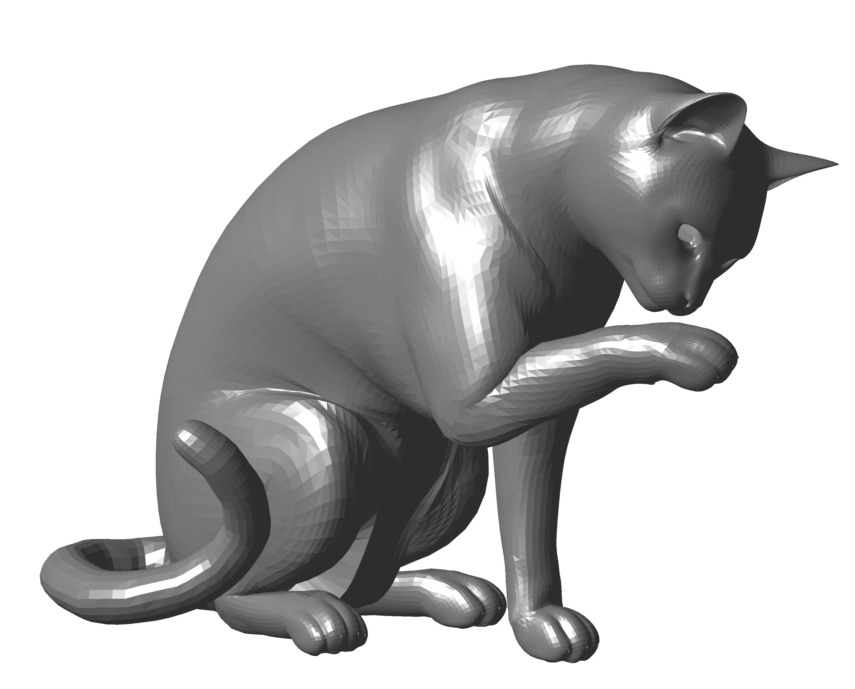
\includegraphics[height=0.85\linewidth]{./fig/eval/cat_mesh.png} 
		\subcaption{Mesh} 
	\end{subfigure}
	\begin{subfigure}[t]{0.31\linewidth} \centering
		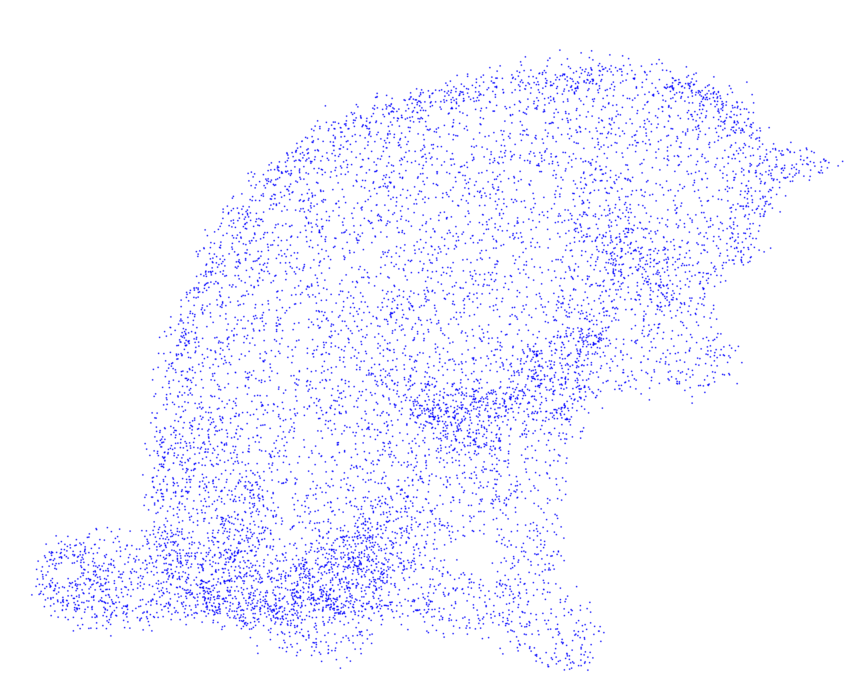
\includegraphics[height=0.85\linewidth]{./fig/eval/cat_points.png}
		\subcaption{Point cloud} 
	\end{subfigure}
	\begin{subfigure}[t]{0.31\linewidth} \centering 
		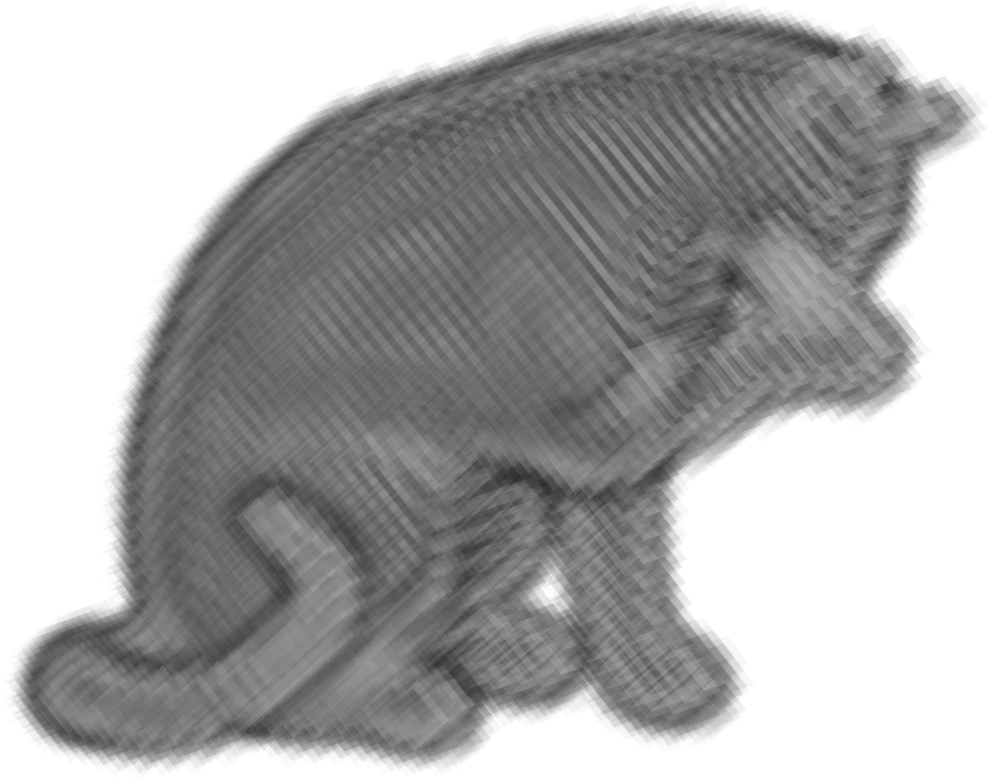
\includegraphics[height=0.85\linewidth]{./fig/eval/cat_volume.png}
		\subcaption{Voxel array} 
	\end{subfigure}
	\caption{Mesh to volume conversion. Left to right: mesh, point cloud and voxel array.} 
	\label{fig/eval/vol_conversion}
\end{figure}

% done 
Three different datasets were used in the evaluation experiments. Two of them were synthetic, as large sets of real, registered, 3D data with known groundtruths were not commonly available. Synthetic data were used because new test data could be generated and modified easily, with controllable noise levels, transformations and sampling densities. Accurate groundtruths were generated with the synthetic test data simultaneously for evaluation.  
From the graphs in figure \ref{fig/eval/graph2}, synthetic and real testing data produced comparable results in the evaluation experiments. 

% done 
The first set, \meshset dataset, contained $25$ shapes (surface meshes) chosen from the Princeton Shape Benchmark \cite{Shilane2004} and TOSCA \cite{Bronstein2008} dataset. 
This dataset contained a wide range of geometric features, ranging from coarse structures to fine details, as illustrated in figure \ref{fig/eval/sampleshapes}. Point clouds were created by sampling 3D points, with a uniform distribution, over the surfaces of the meshes. Gaussian white noise was added to the points to simulate measurement errors introduced during 3D shape acquisition. 
The point clouds were subsequently voxelised to volumetric data using kernel density estimation with a Gaussian kernel $g(\cdot,\sigma_{KDE})$, as illustrated in figure \ref{fig/eval/vol_conversion}.
%This conversion process allows sampling density and noise to be varied when generating the volumes.
Finally, a linear scale-space $\mathbf{v}(\mathbf{x};\sigma_s)$ is created from each volume, in order to detect shape features at different scales, \cf \ref{sec/eval/subvoxel}. All shapes in the dataset undergo this conversion process. 

% done 
The \mriset dataset consisted of two synthetic MRI scans of a human brain, generated from BrainWeb simulated brain database \cite{Cocosco1997}. The groundtruth homographies ($20^{\circ}$ rotation and $20$ voxel translation) between the two MRI scans were given for performance evaluation. The MRI scans were inherently volumetric, thus no voxelisation process was involved. 

% done 
The third dataset, \stereoset, was a series of $16$ point clouds of $8$ objects from the Toshiba CAD model point clouds dataset \cite{Pham2011}, which was captured using a photometric, multi-view stereo system \cite{Vogiatzis2011}. Relative transformations were computed by aligning each point cloud with a reference model using the ICP algorithm \cite{Besl1992} and then refining the registrating manually. The same voxelisation technique was used to convert stereo point clouds to volumetric data.

% done 
In \meshset and \stereoset datasets, high-intensity voxels were only located at the object surface, leaving the interior of the shapes hollow as low-intensity voxels. In contrast, the interior of the \mriset data was filled with voxels of different intensity. The experimental results have demonstrated different behaviours of the detectors in these two voxelisation scenarios.

% done 
While the synthetic shape instances of the same object completely overlapped one another, avoiding bias to the repeatability score mentioned in Willis and Sui \cite{Willis2009}, the real stereo data contained occlusions. While the underside of each object, which varied across instances, was not captured, the shapes in \stereoset were captured with uneven sampling density and generally more sampling noise. The feasibility of performance evaluation using synthetic data was therefore verified by comparing the results on the \meshset dataset with those on the \stereoset dataset. 

%\begin{figure}[ht]
%\centering
%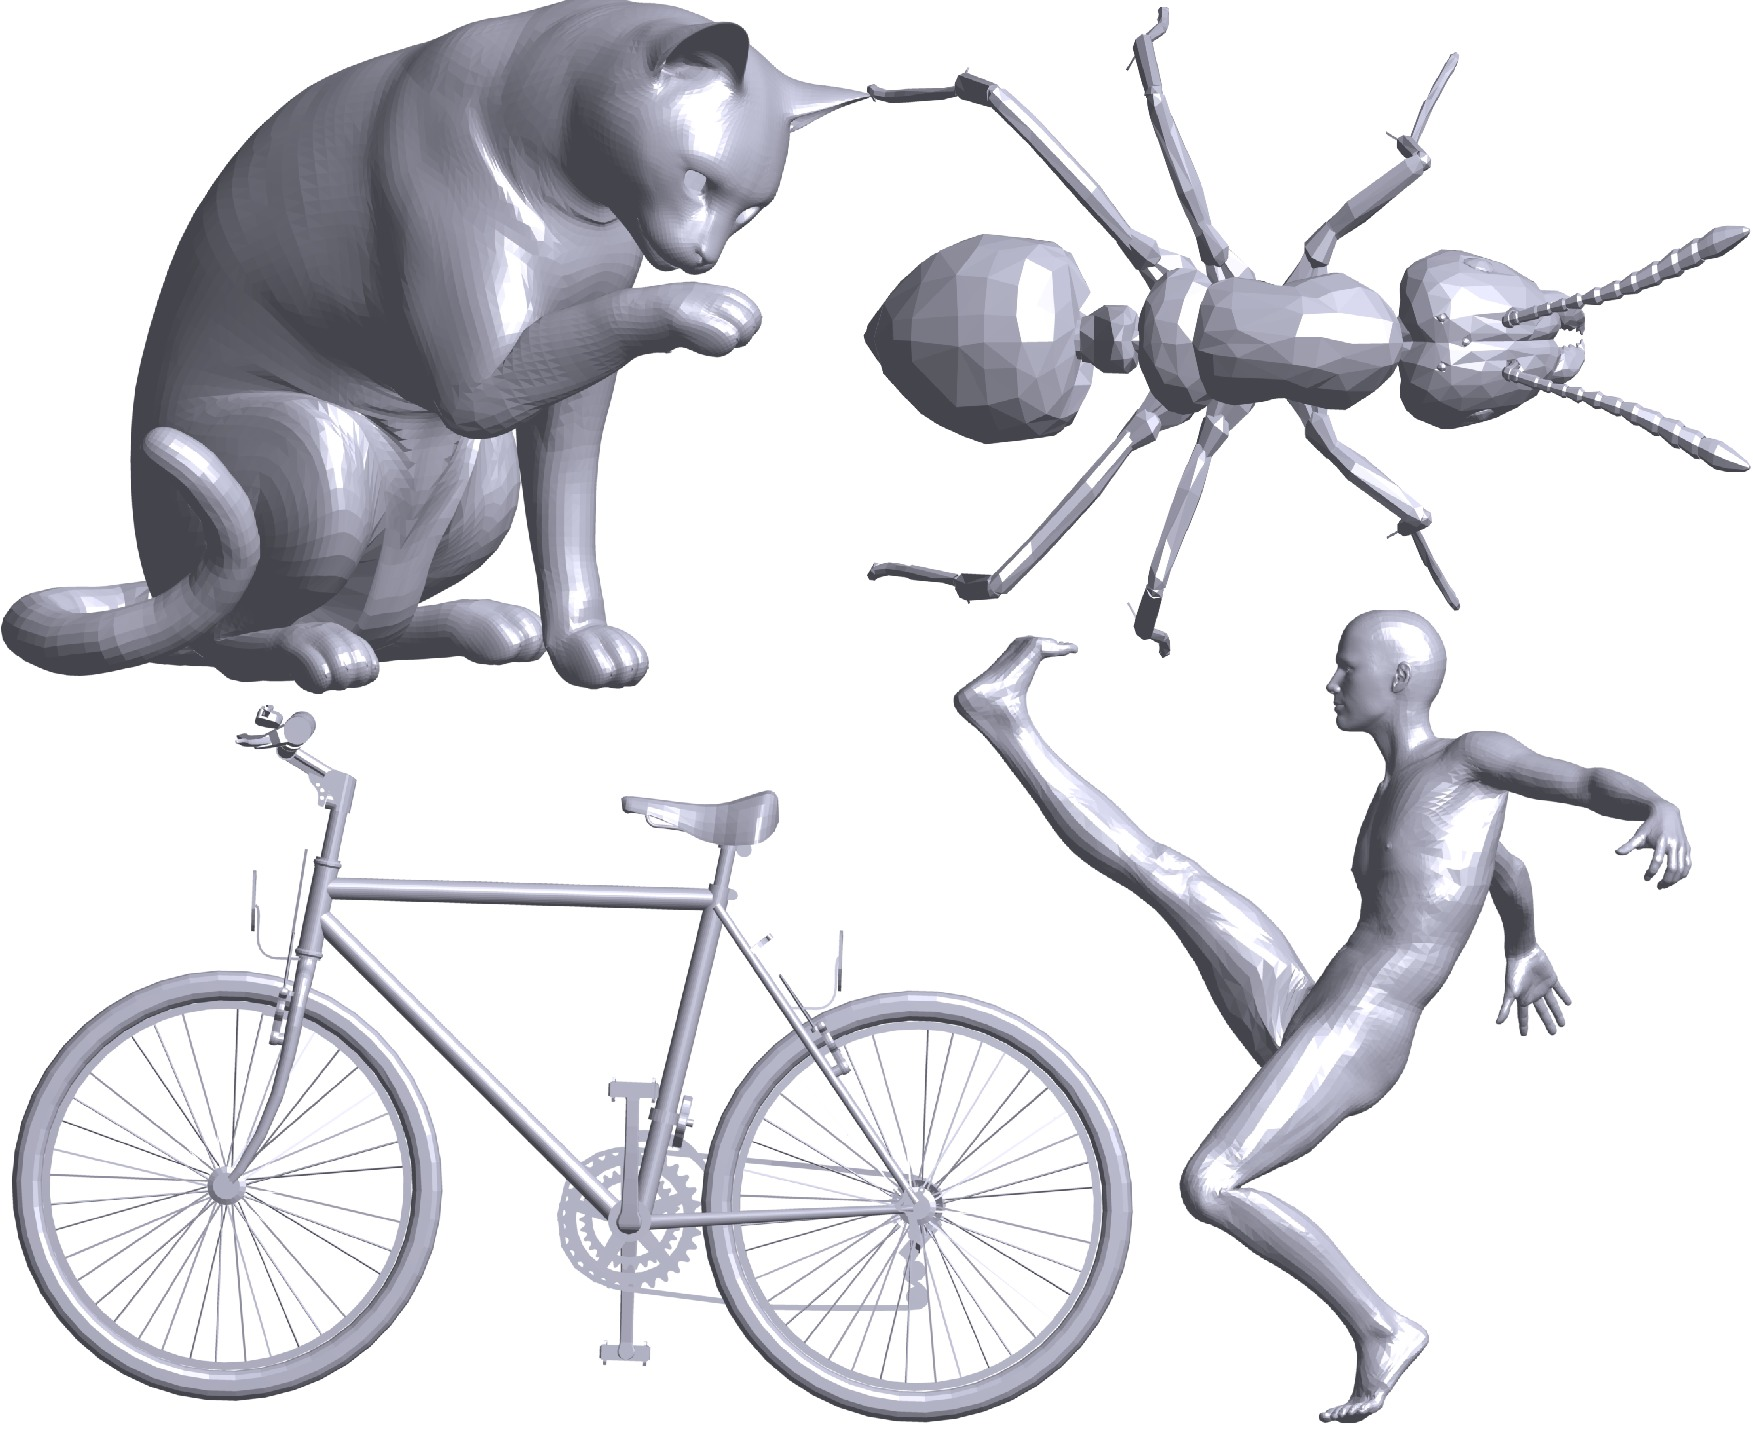
\includegraphics[width=0.75\linewidth]{./fig/eval/sampleshape.pdf}
%\caption{Example shapes taken from the \meshset dataset.} 
%\label{fig/eval/sampleshapes}
%\end{figure}

\begin{figure}
	\begin{subfigure}[t]{0.19\linewidth} \centering
		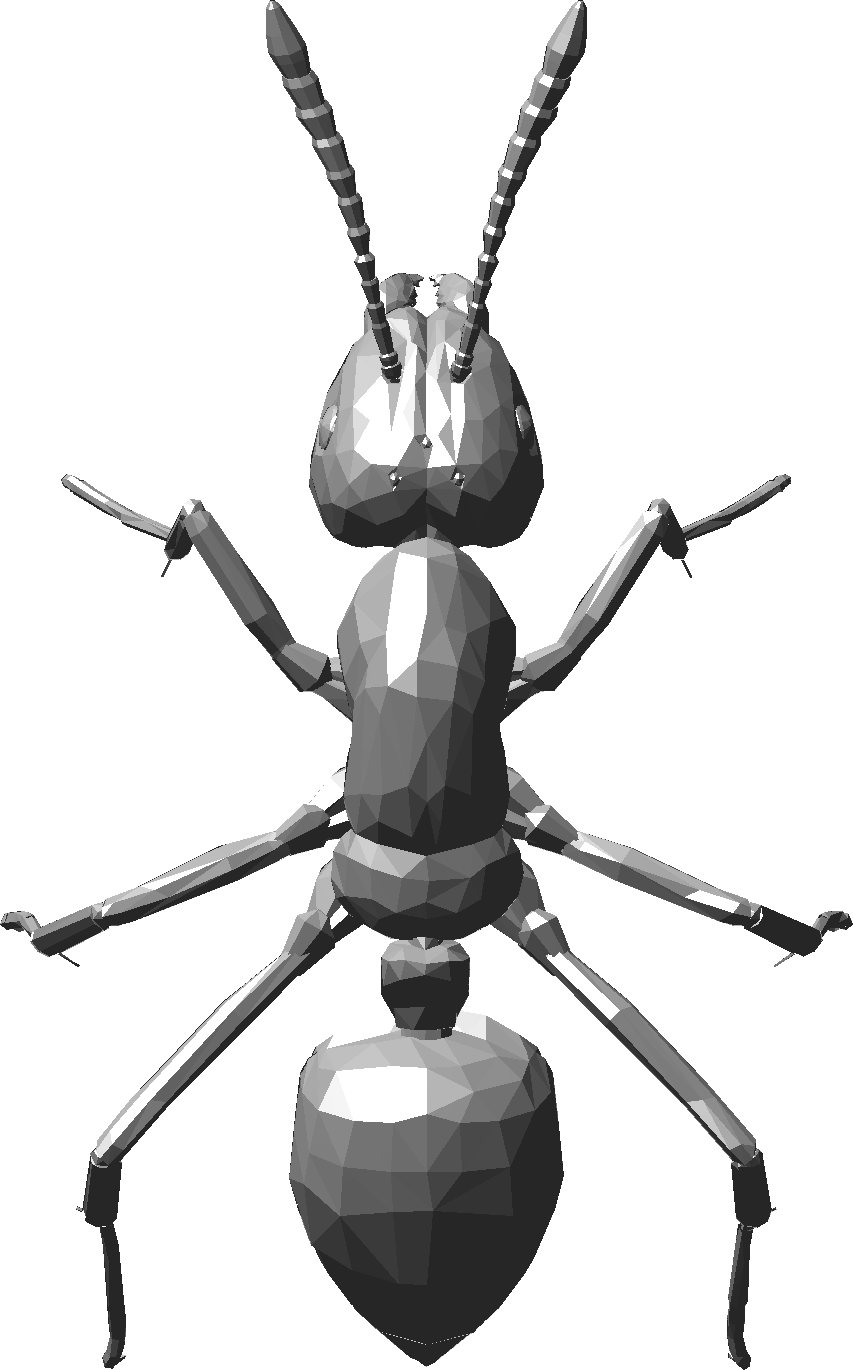
\includegraphics[width=0.7\linewidth]{./fig/eval/01ant.png}  
		\caption{Ant} 	
	\end{subfigure}
	\begin{subfigure}[t]{0.19\linewidth} \centering
		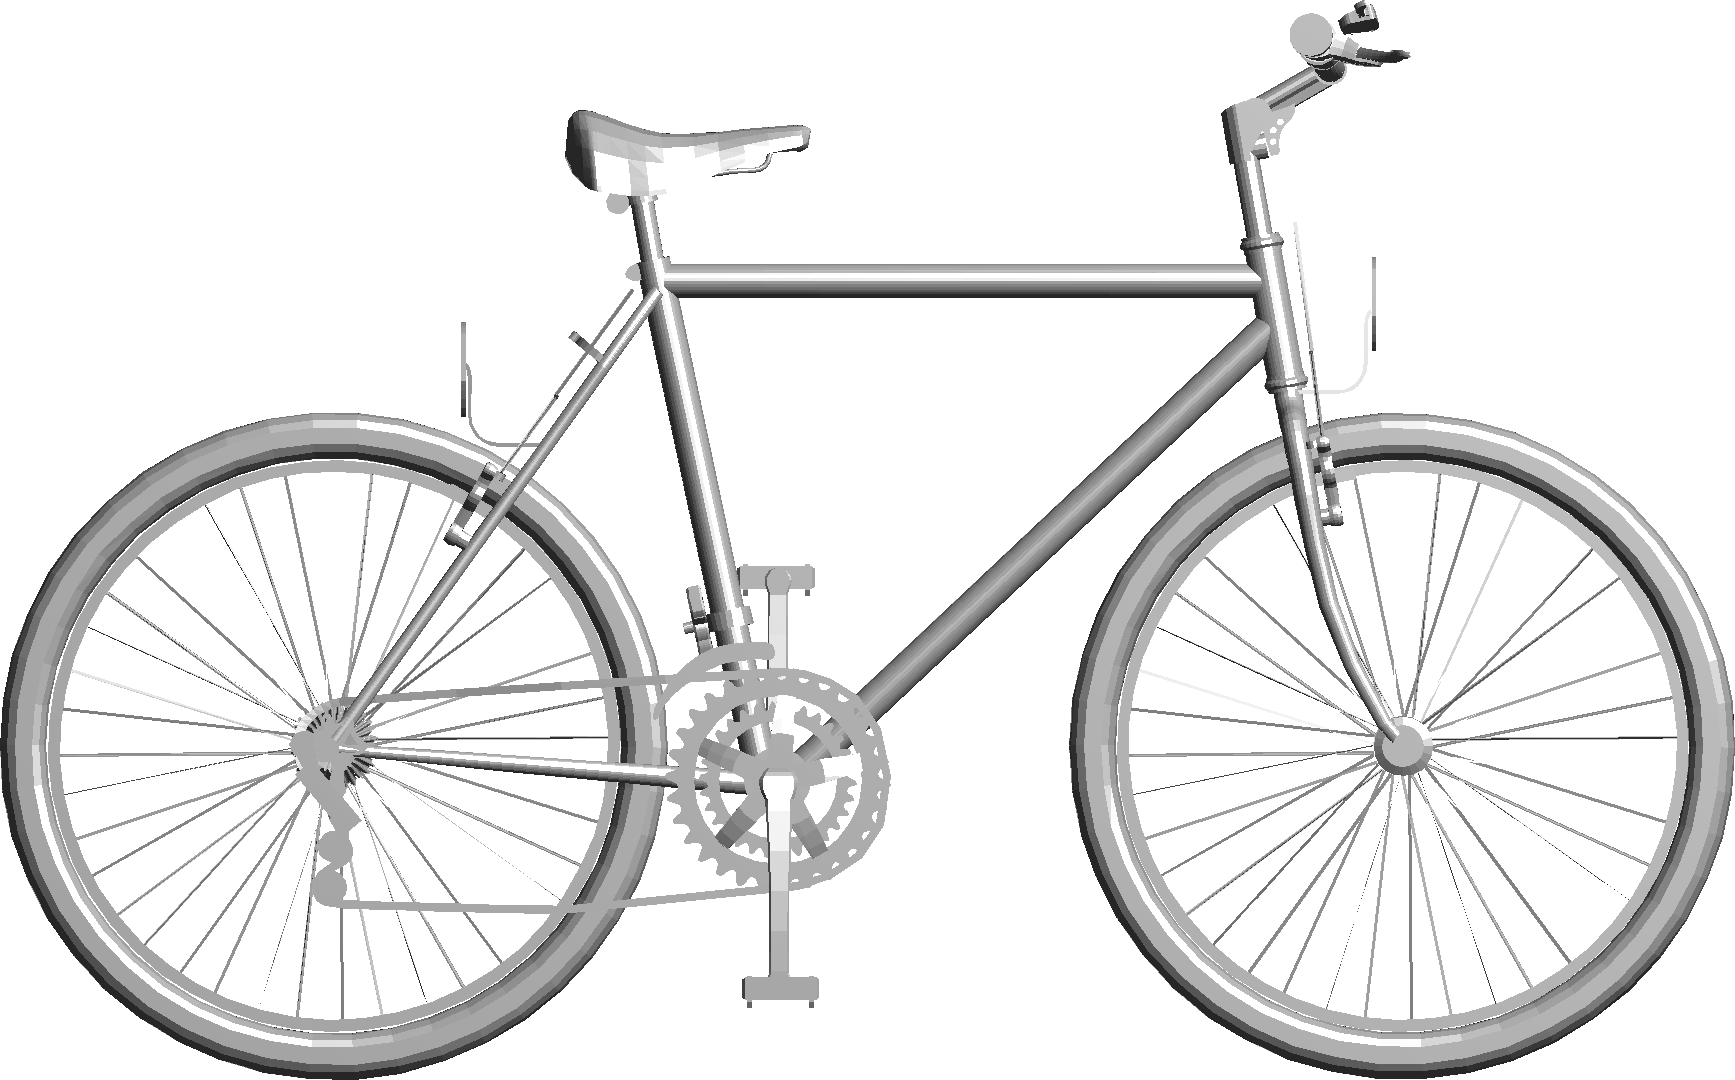
\includegraphics[width=1\linewidth]{./fig/eval/02bicycle.png}  
		\caption{Bicycle} 	
	\end{subfigure}
	\begin{subfigure}[t]{0.19\linewidth} \centering
		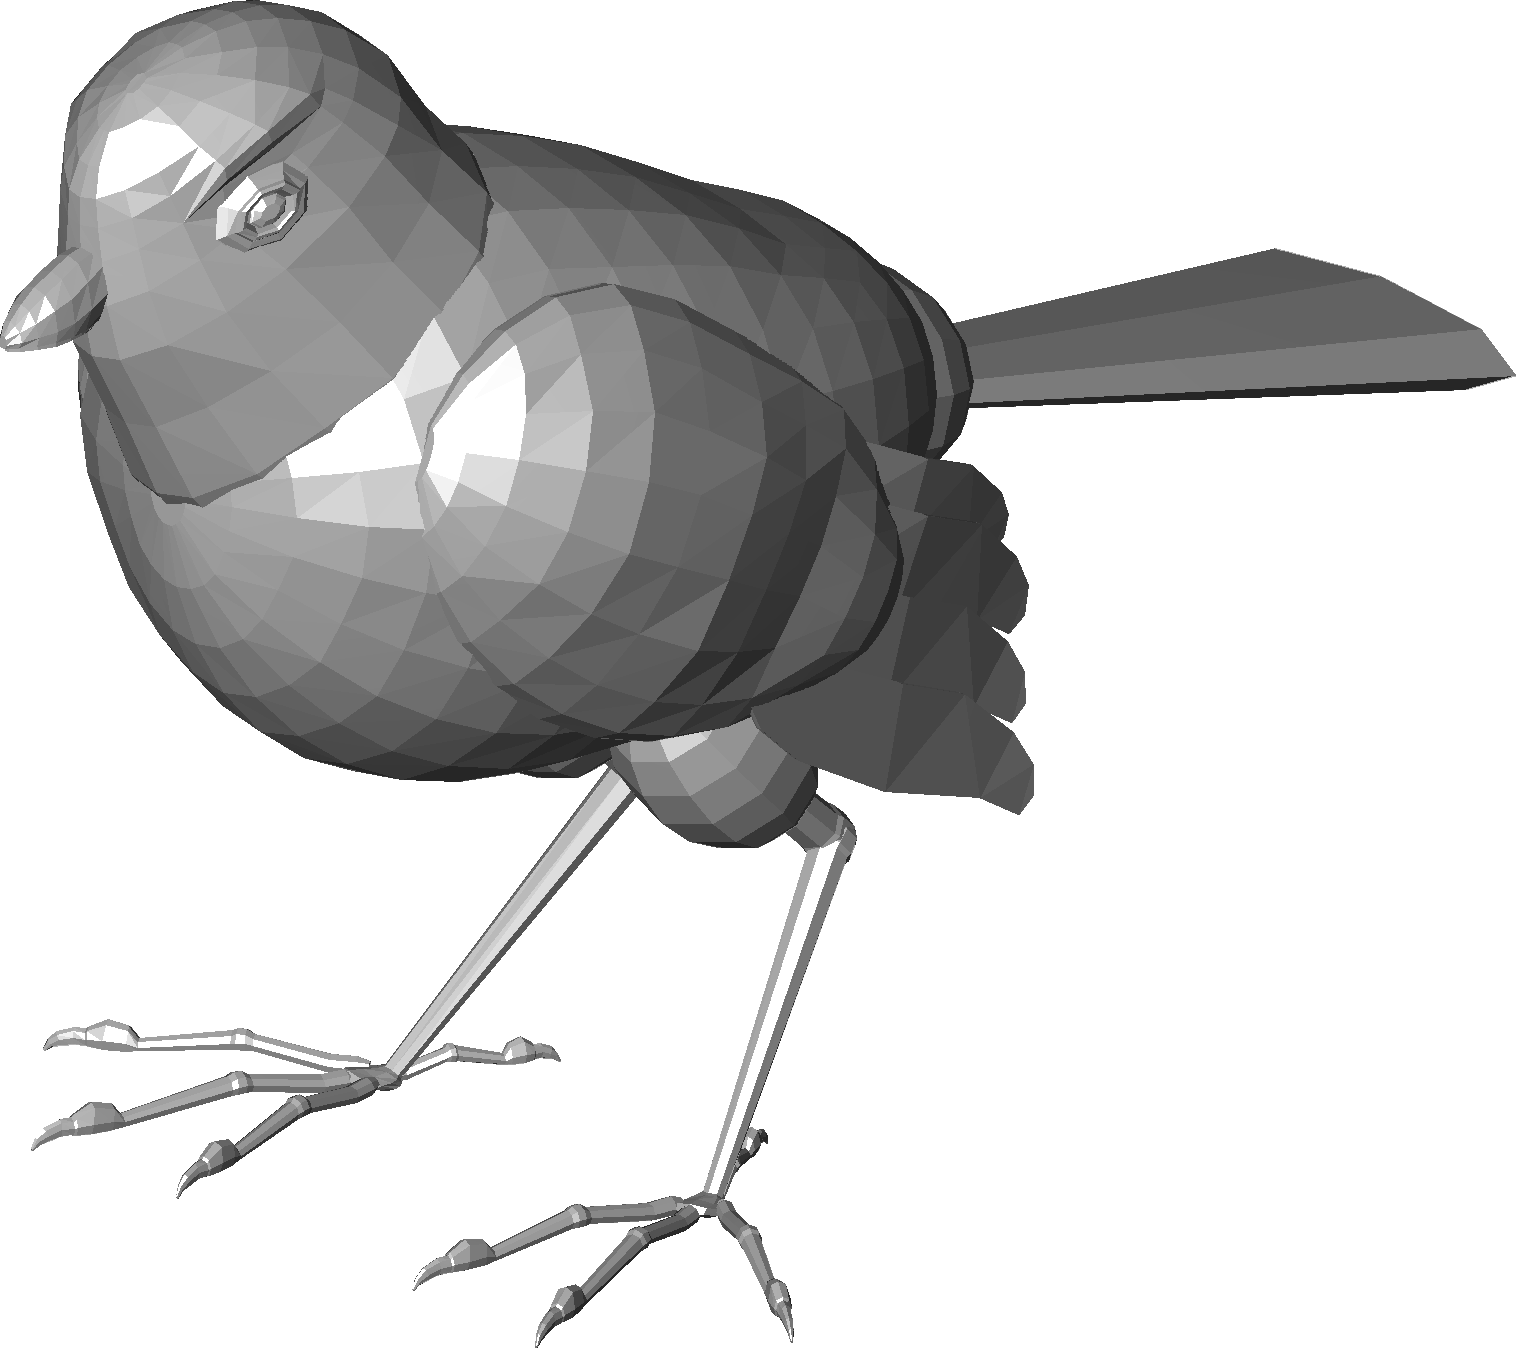
\includegraphics[width=1\linewidth]{./fig/eval/03bird.png}  
		\caption{Bird} 	
	\end{subfigure}
	\begin{subfigure}[t]{0.19\linewidth} \centering
		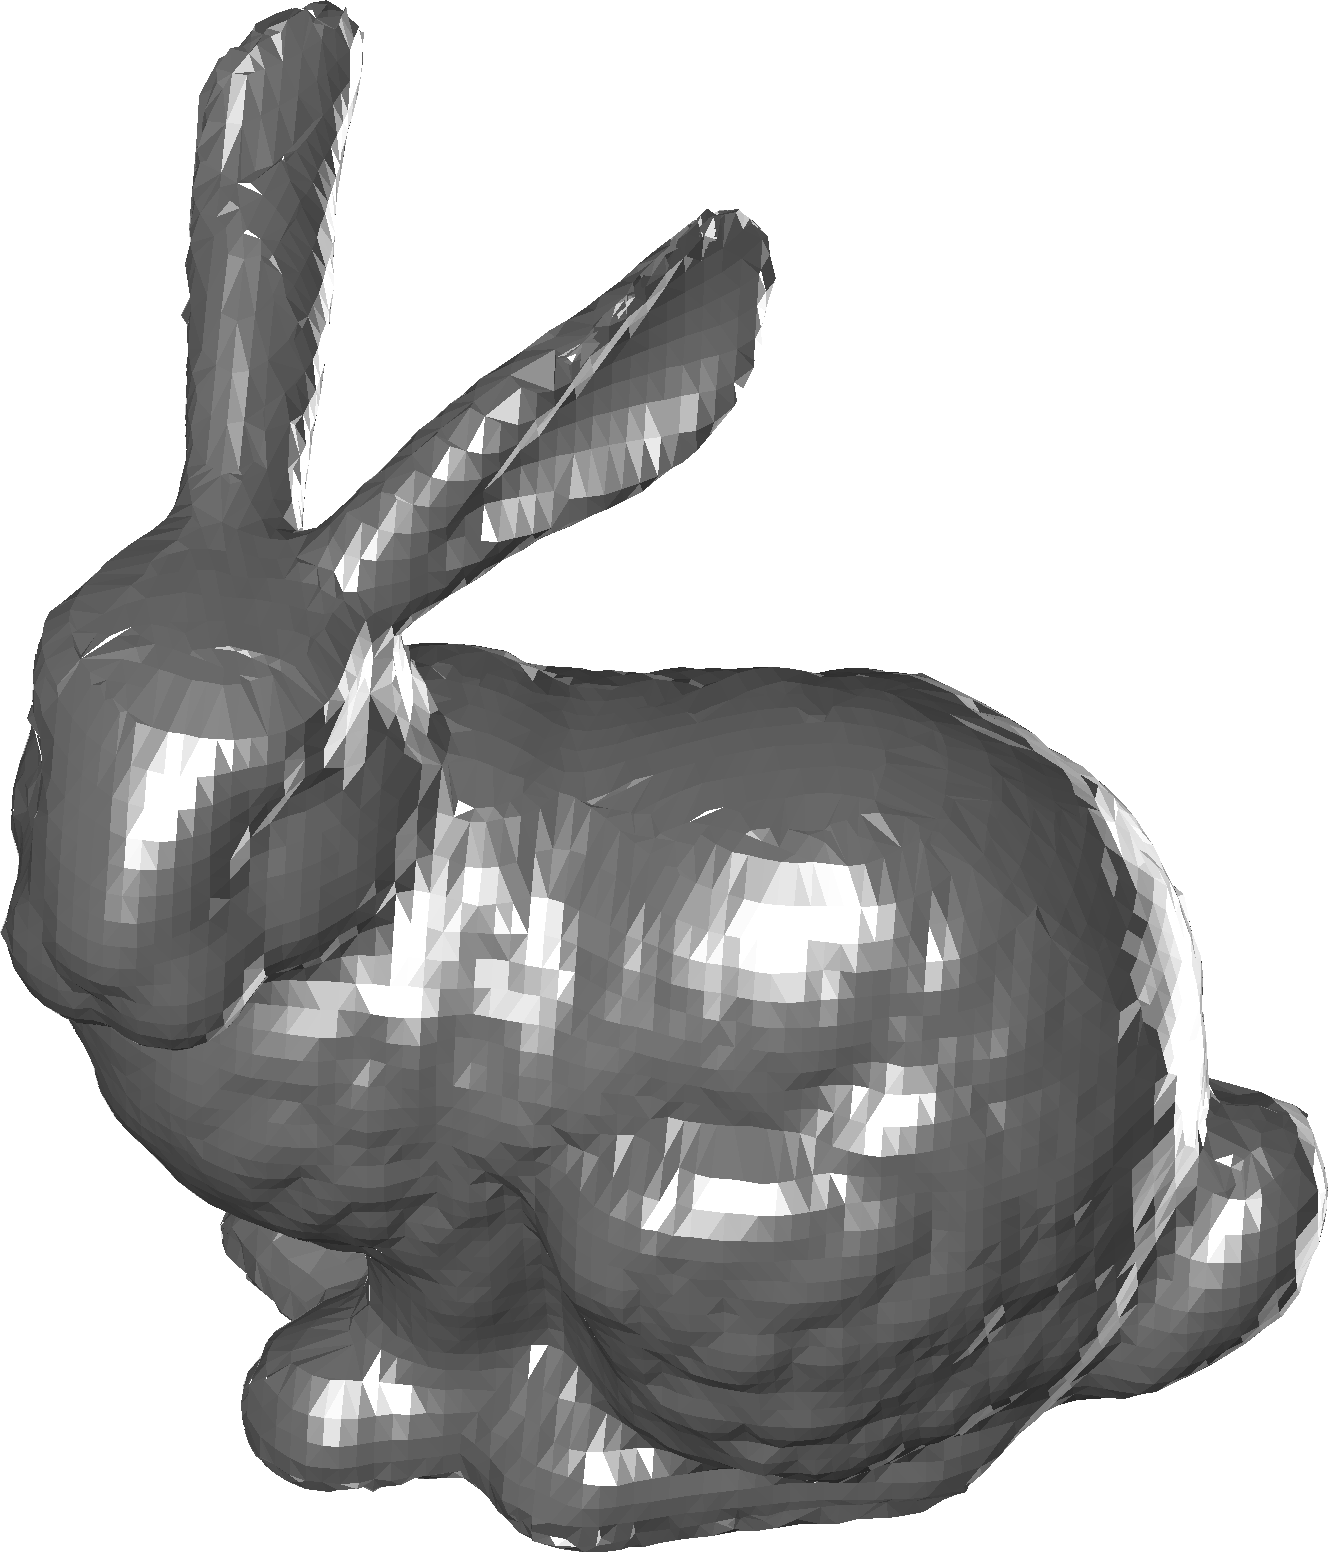
\includegraphics[width=0.9\linewidth]{./fig/eval/04bunny.png}  
		\caption{Bunny} 	
	\end{subfigure} 
	\begin{subfigure}[t]{0.19\linewidth} \centering
		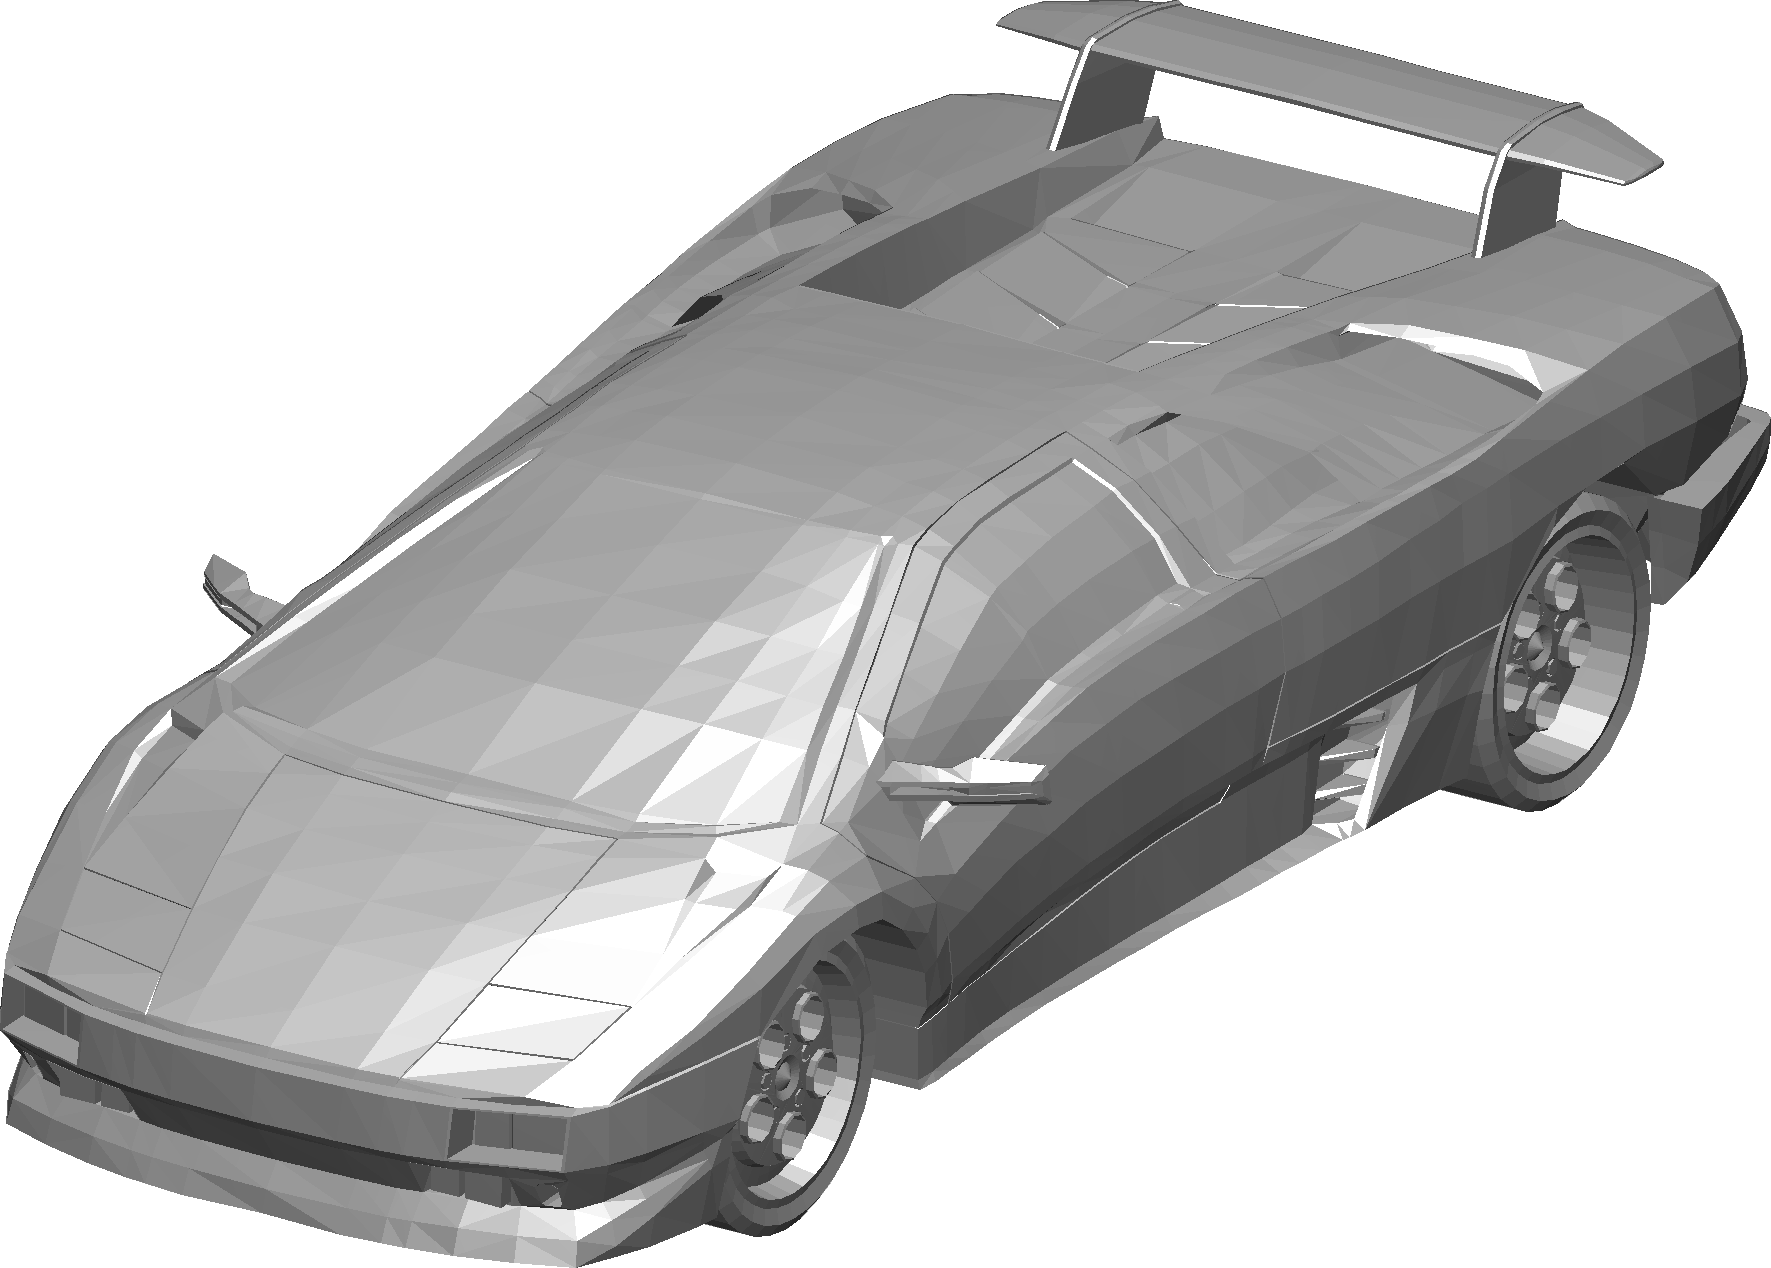
\includegraphics[width=1\linewidth]{./fig/eval/05car.png}  
		\caption{Car} 	
	\end{subfigure} \\ 
	\begin{subfigure}[t]{0.19\linewidth} \centering
		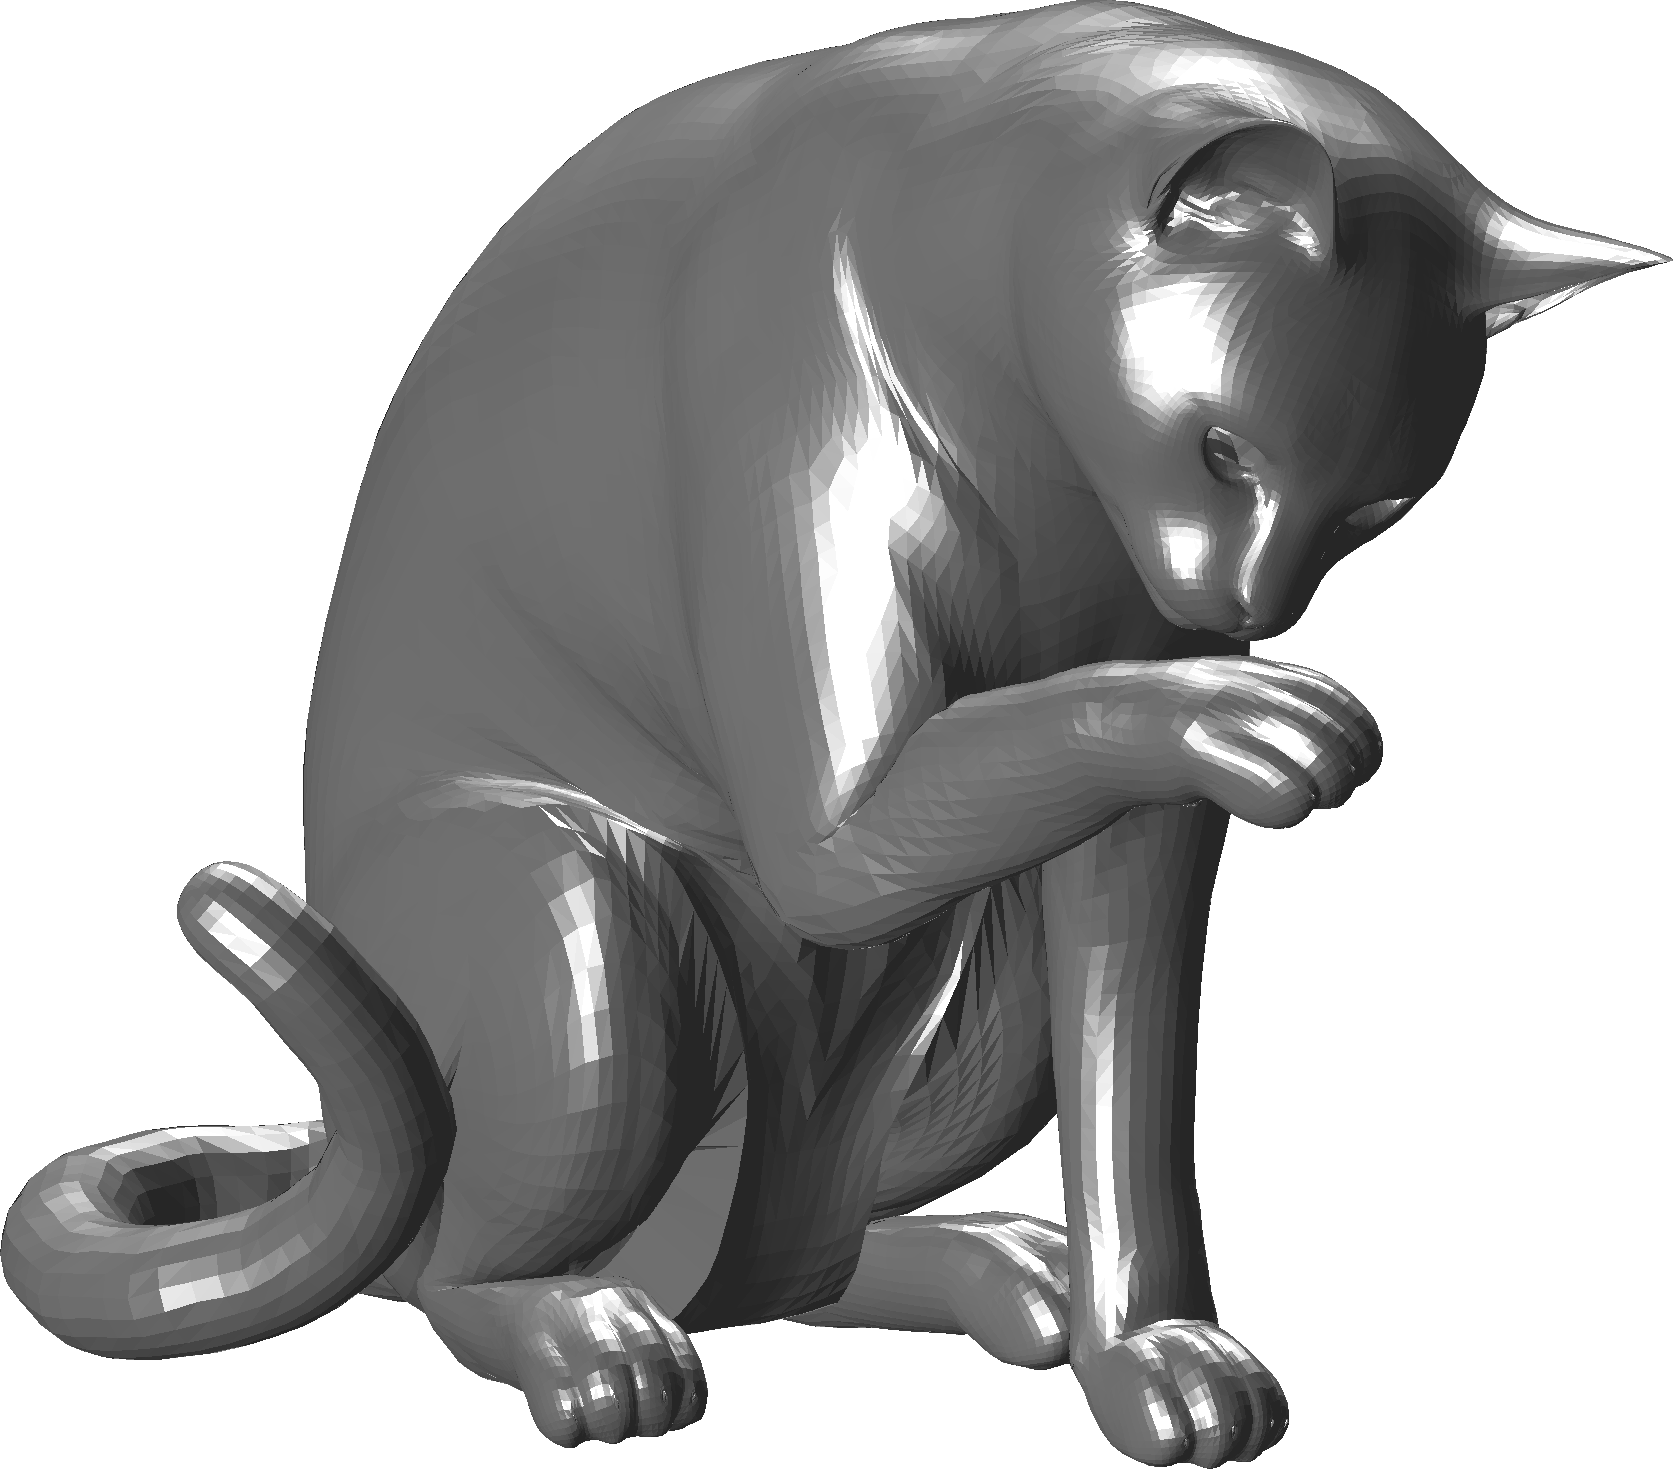
\includegraphics[width=1\linewidth]{./fig/eval/06cat.png}  
		\caption{Cat} 	
	\end{subfigure}
	\begin{subfigure}[t]{0.19\linewidth} \centering
		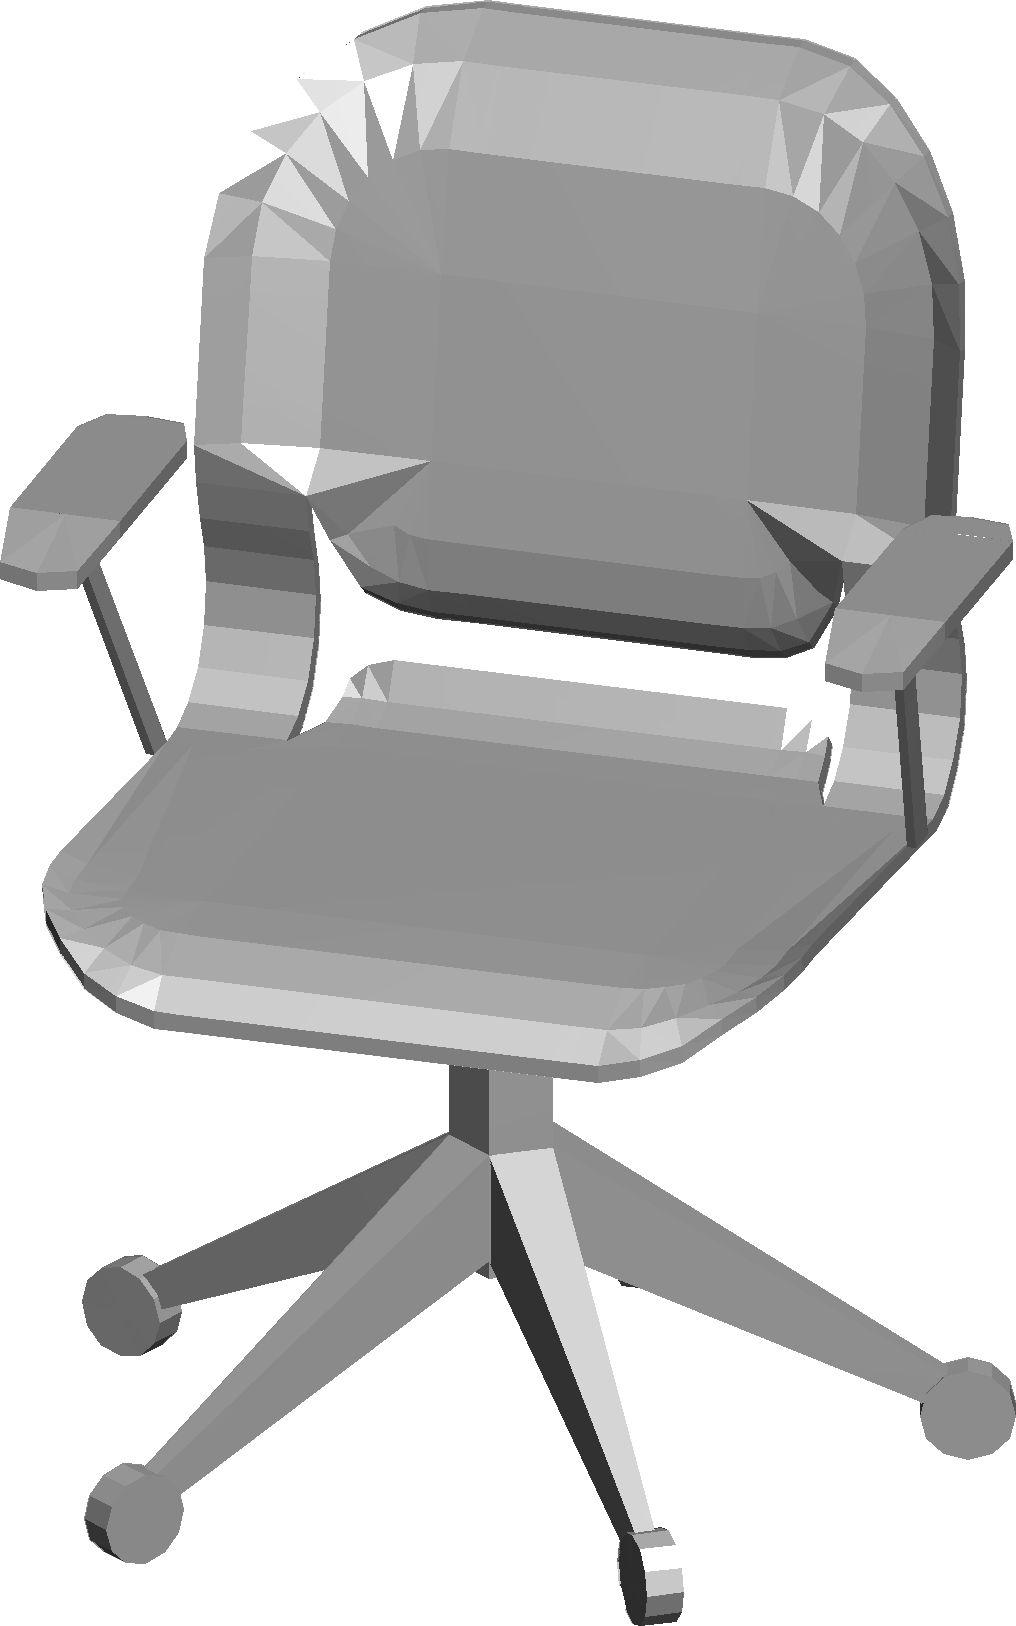
\includegraphics[width=0.7\linewidth]{./fig/eval/07chair.png}  
		\caption{Chair} 	
	\end{subfigure}
	\begin{subfigure}[t]{0.19\linewidth} \centering
		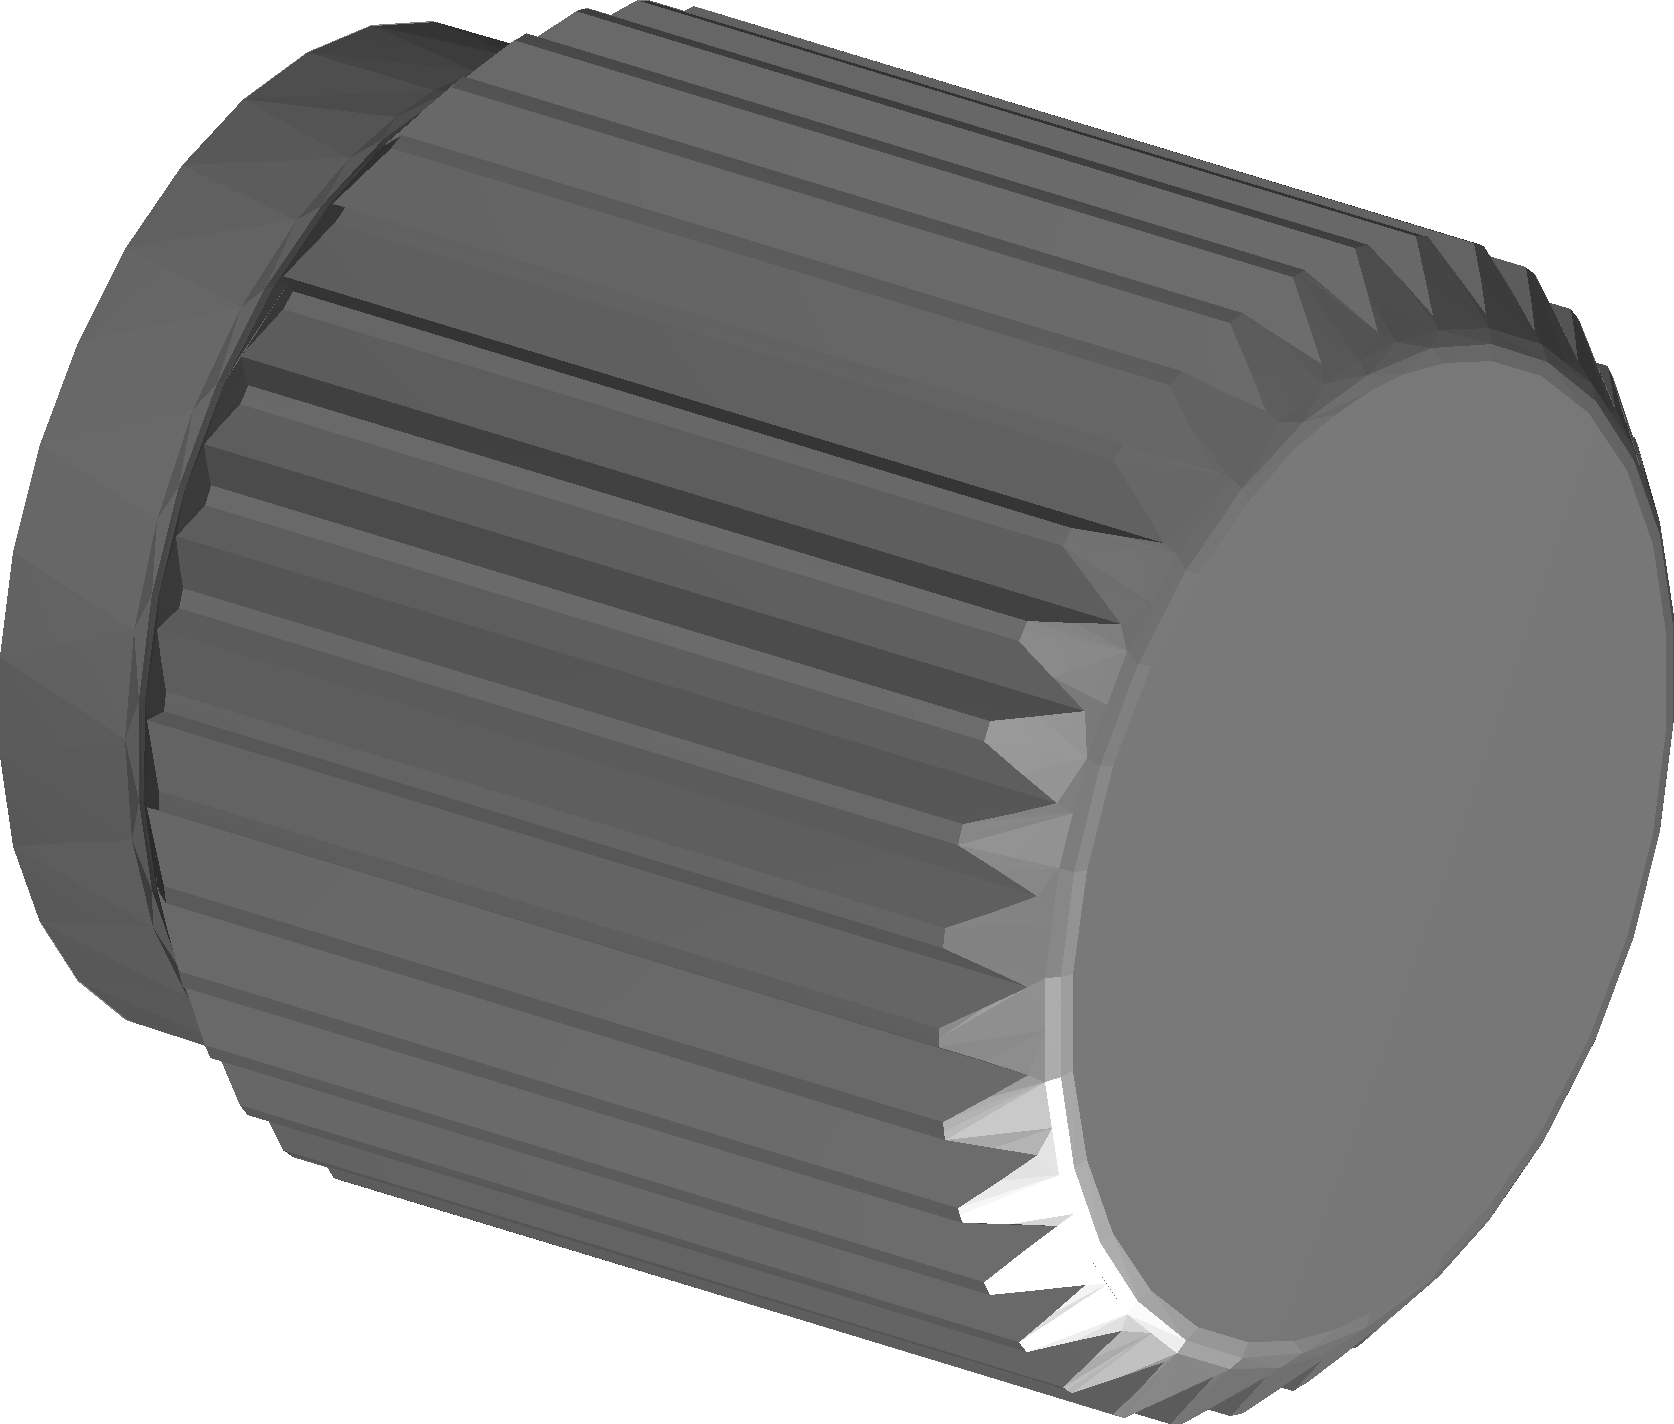
\includegraphics[width=1\linewidth]{./fig/eval/08cog.png}  
		\caption{Cog} 	
	\end{subfigure}
	\begin{subfigure}[t]{0.19\linewidth} \centering
		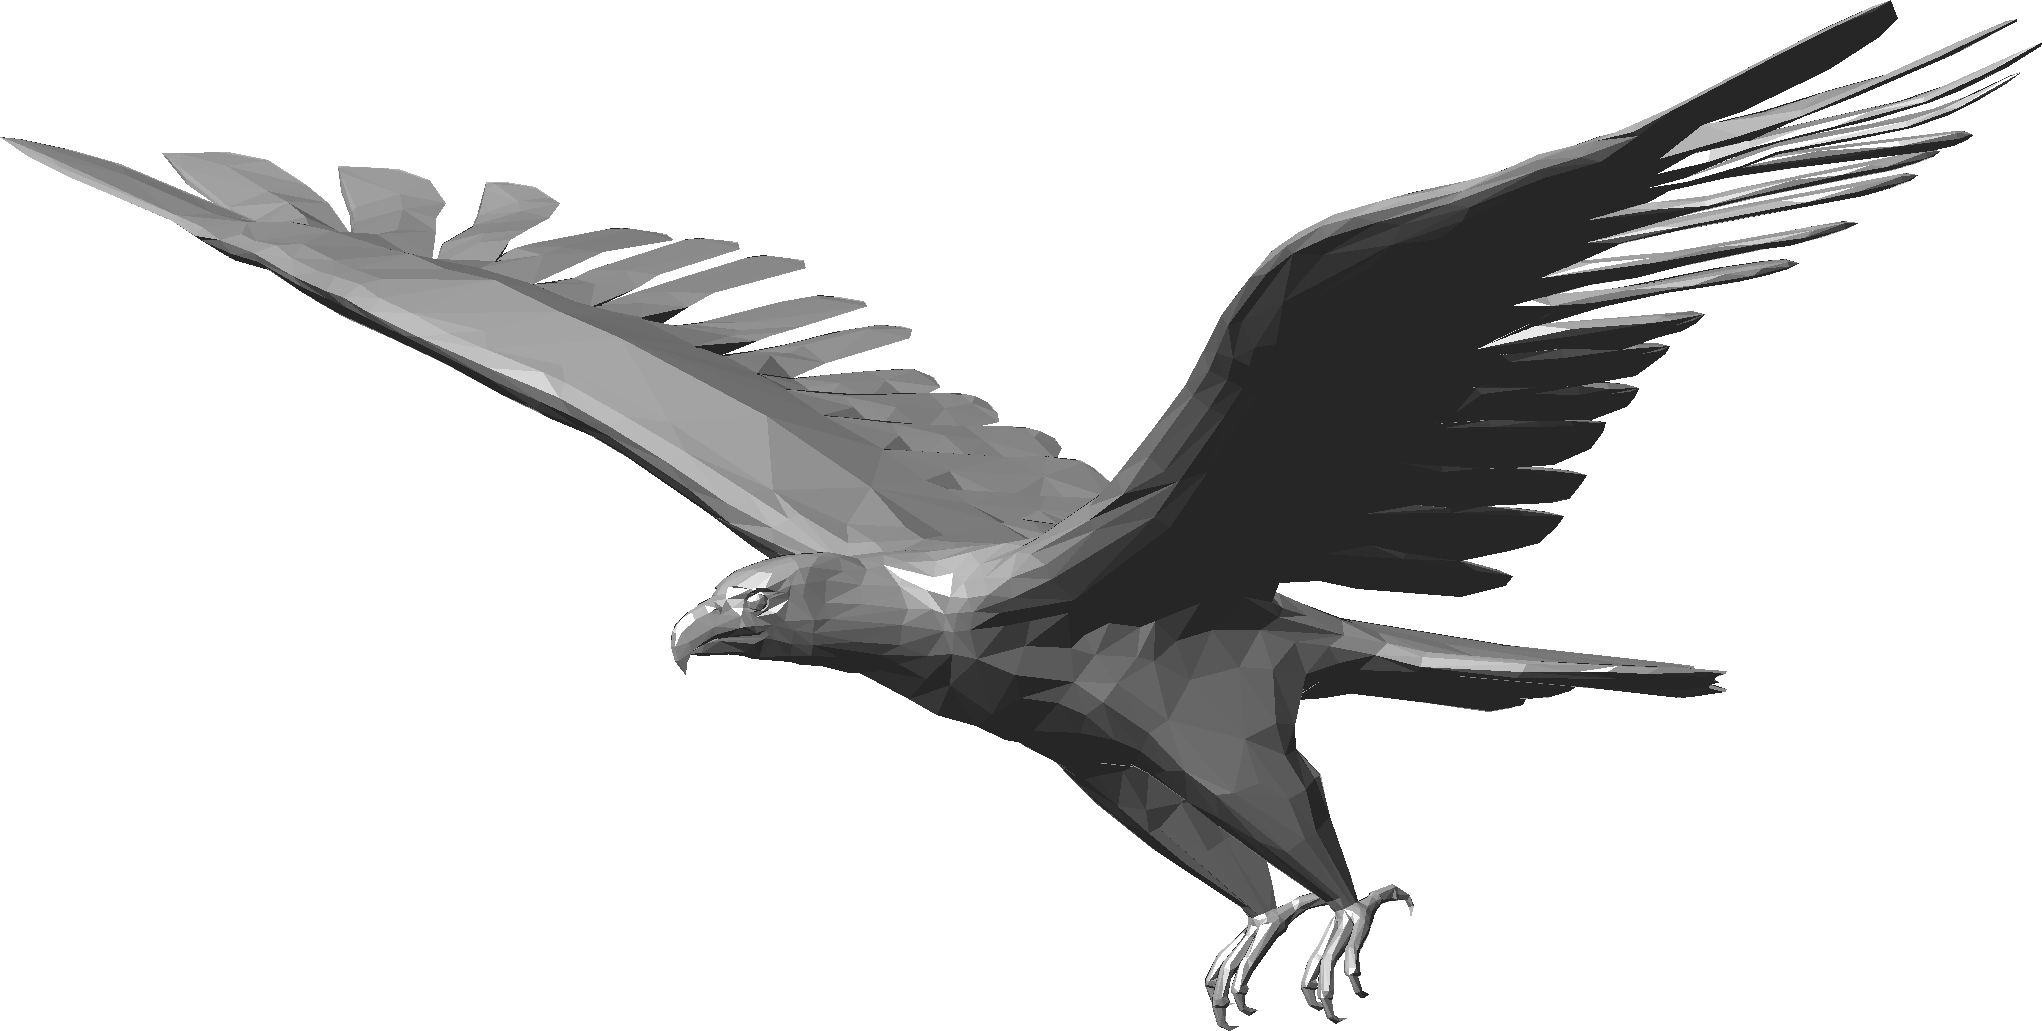
\includegraphics[width=1\linewidth]{./fig/eval/09eagle.png}  
		\caption{Eagle} 	
	\end{subfigure} 
	\begin{subfigure}[t]{0.19\linewidth} \centering
		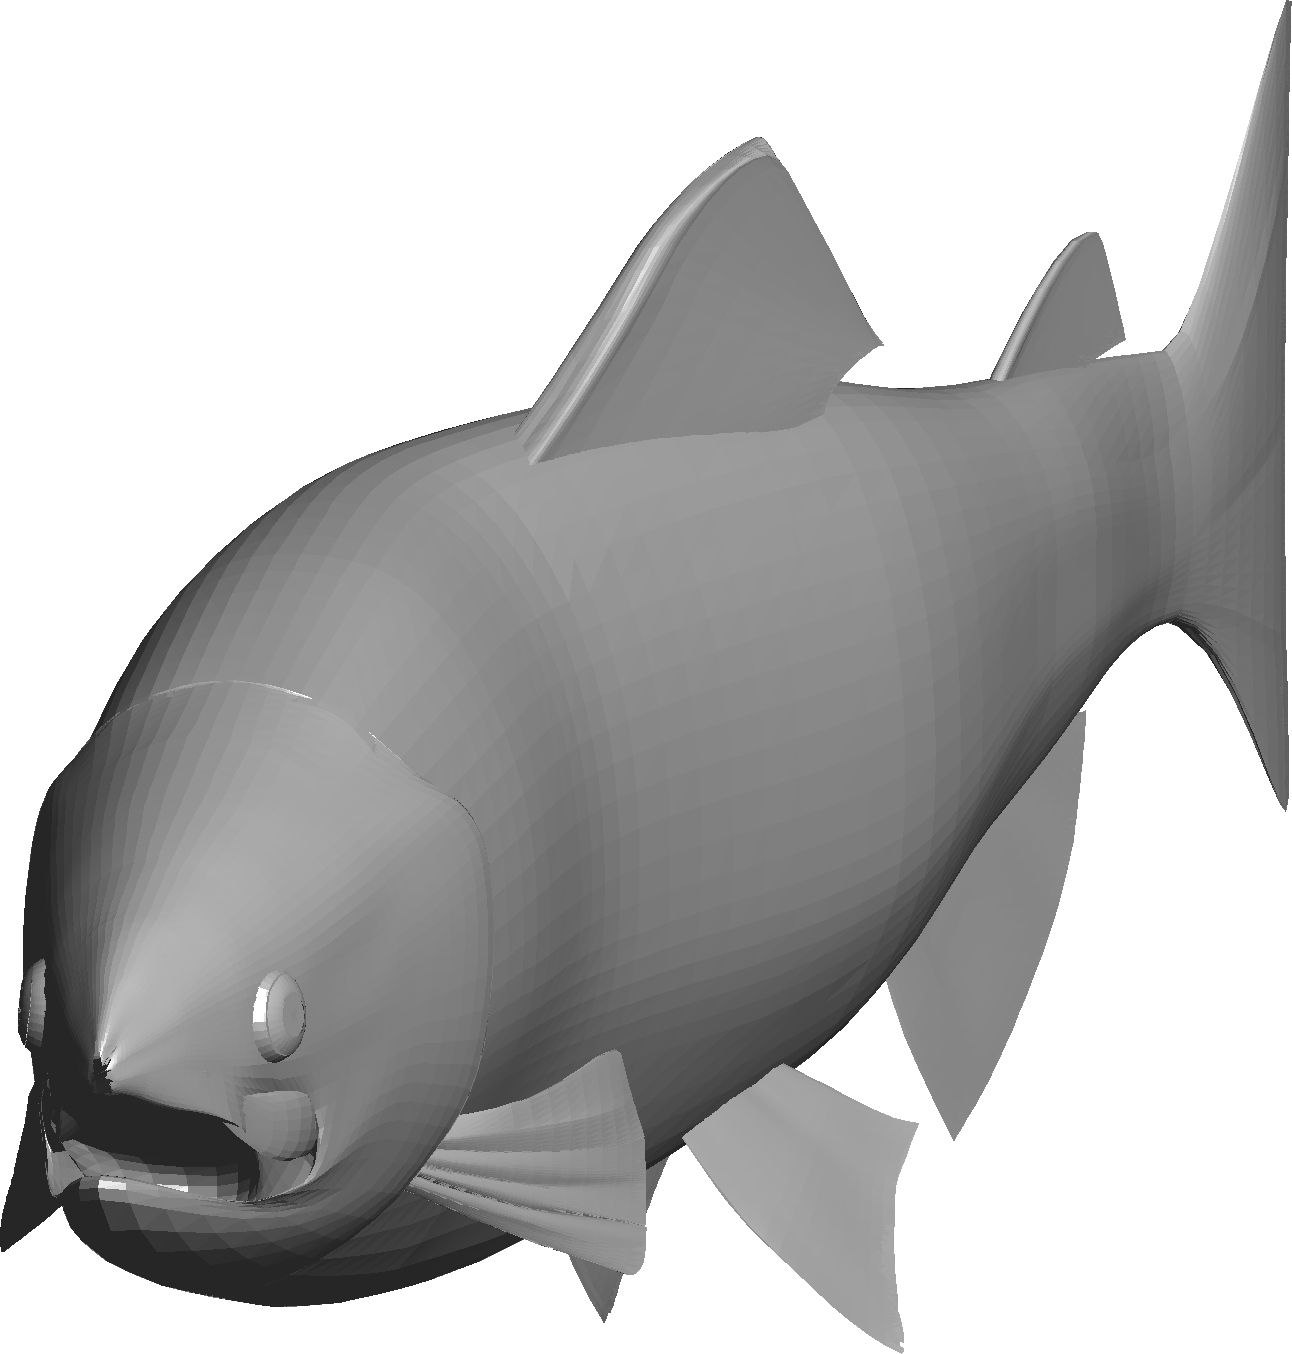
\includegraphics[width=1\linewidth]{./fig/eval/10fish.png}  
		\caption{Fish} 	
	\end{subfigure} \\ 
	\begin{subfigure}[t]{0.19\linewidth} \centering
		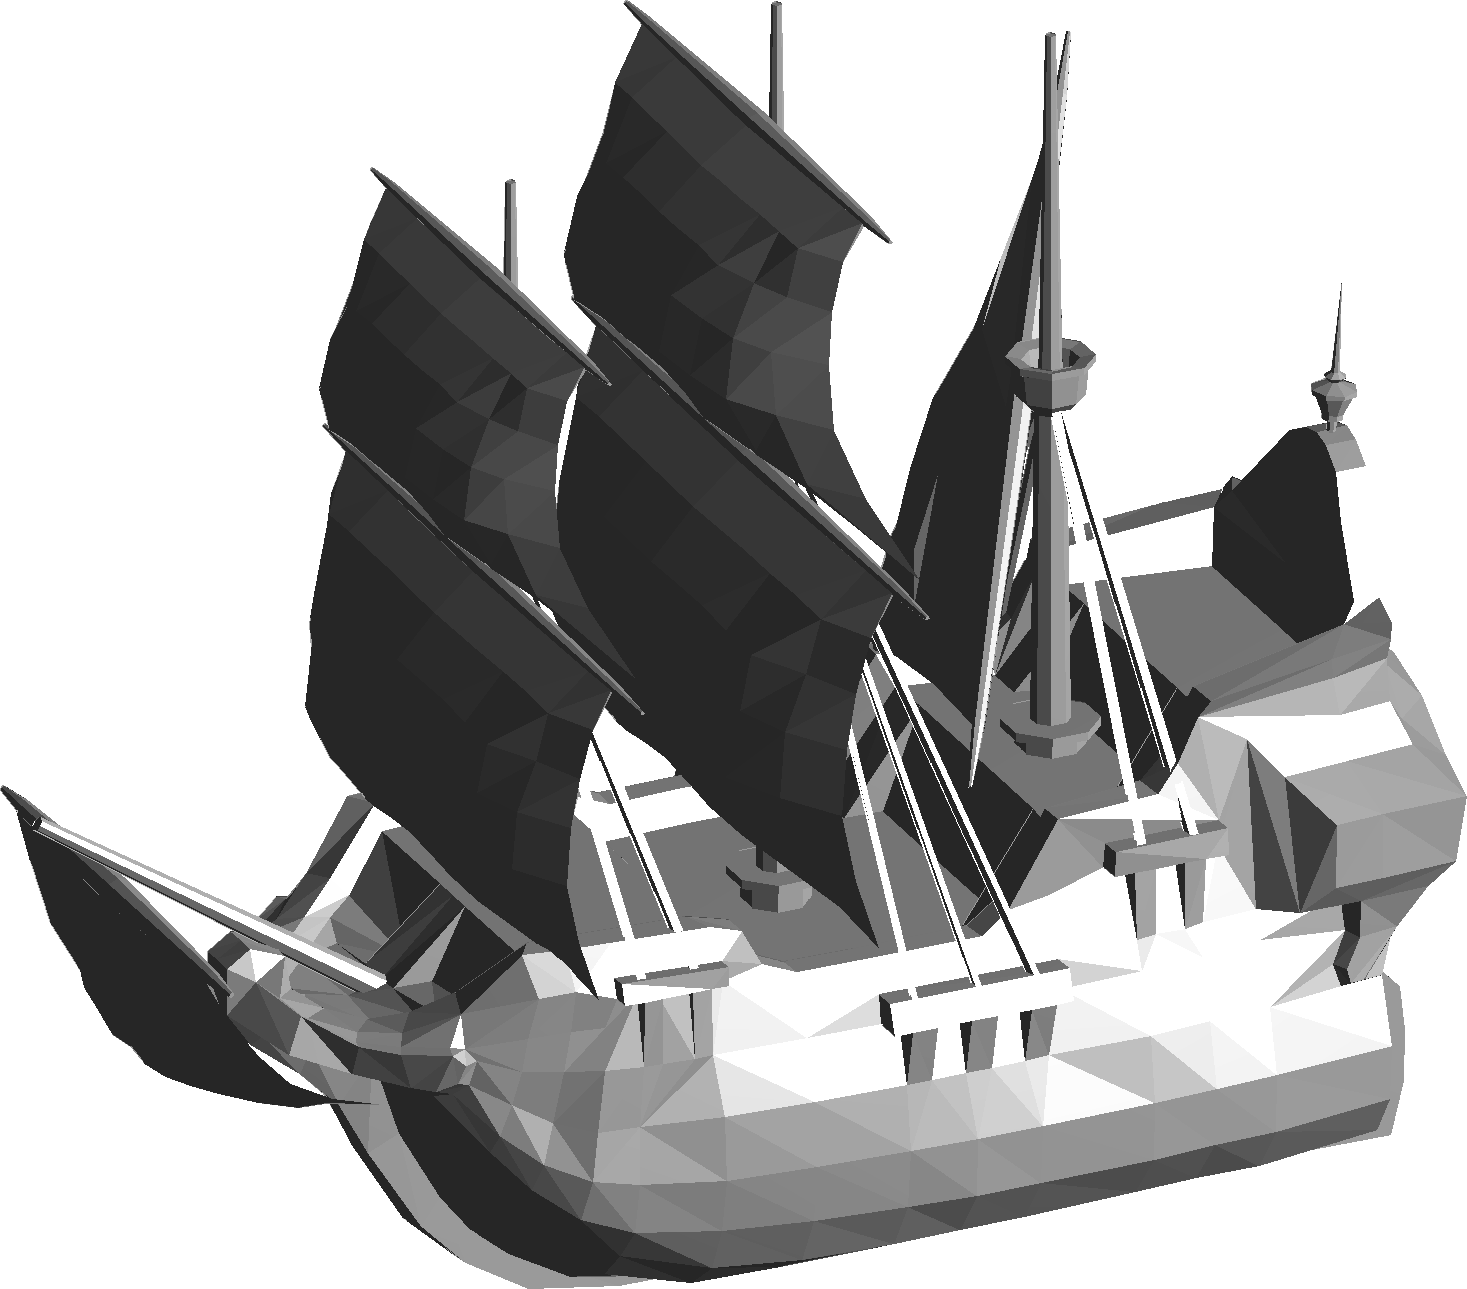
\includegraphics[width=1\linewidth]{./fig/eval/11galleon.png}  
		\caption{Galleon} 	
	\end{subfigure}
	\begin{subfigure}[t]{0.19\linewidth} \centering
		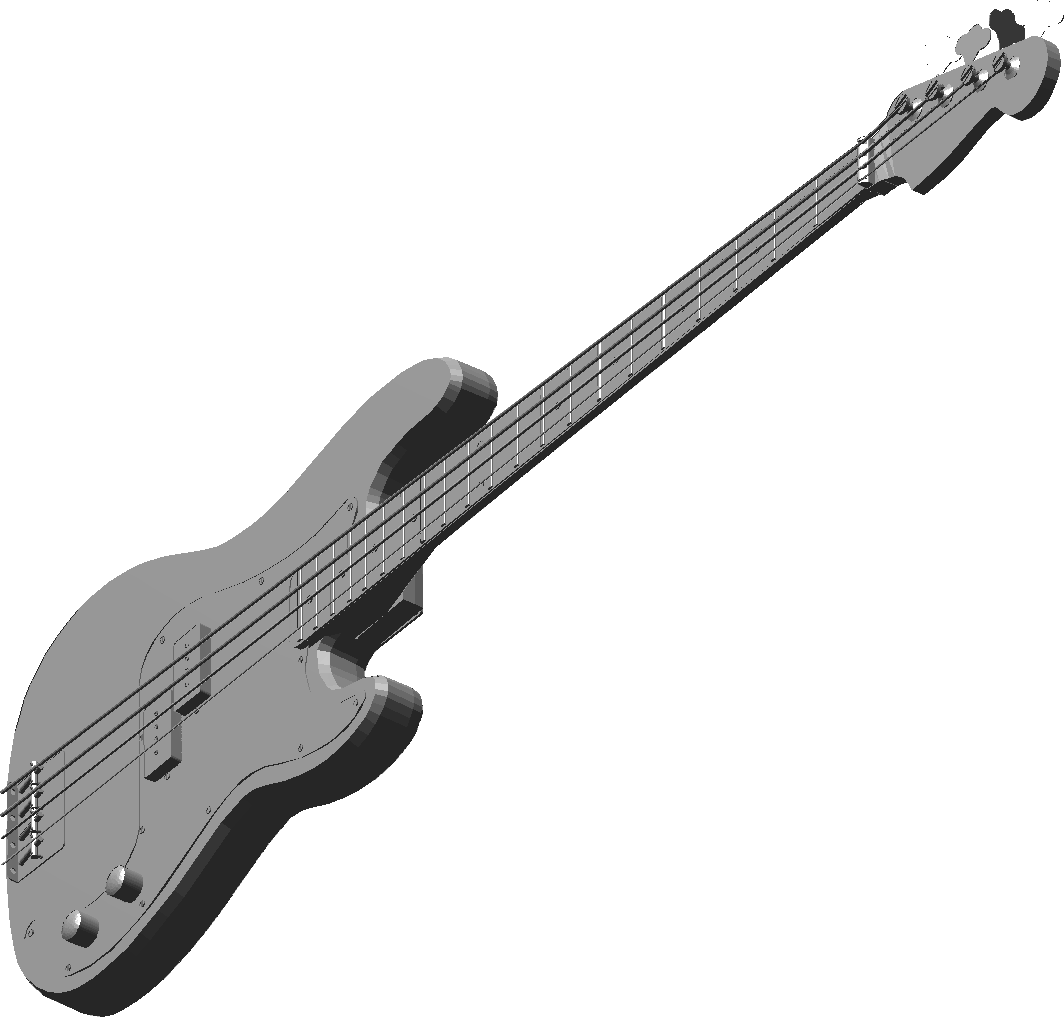
\includegraphics[width=1\linewidth]{./fig/eval/12guitar.png}  
		\caption{Guitar} 	
	\end{subfigure}
	\begin{subfigure}[t]{0.19\linewidth} \centering
		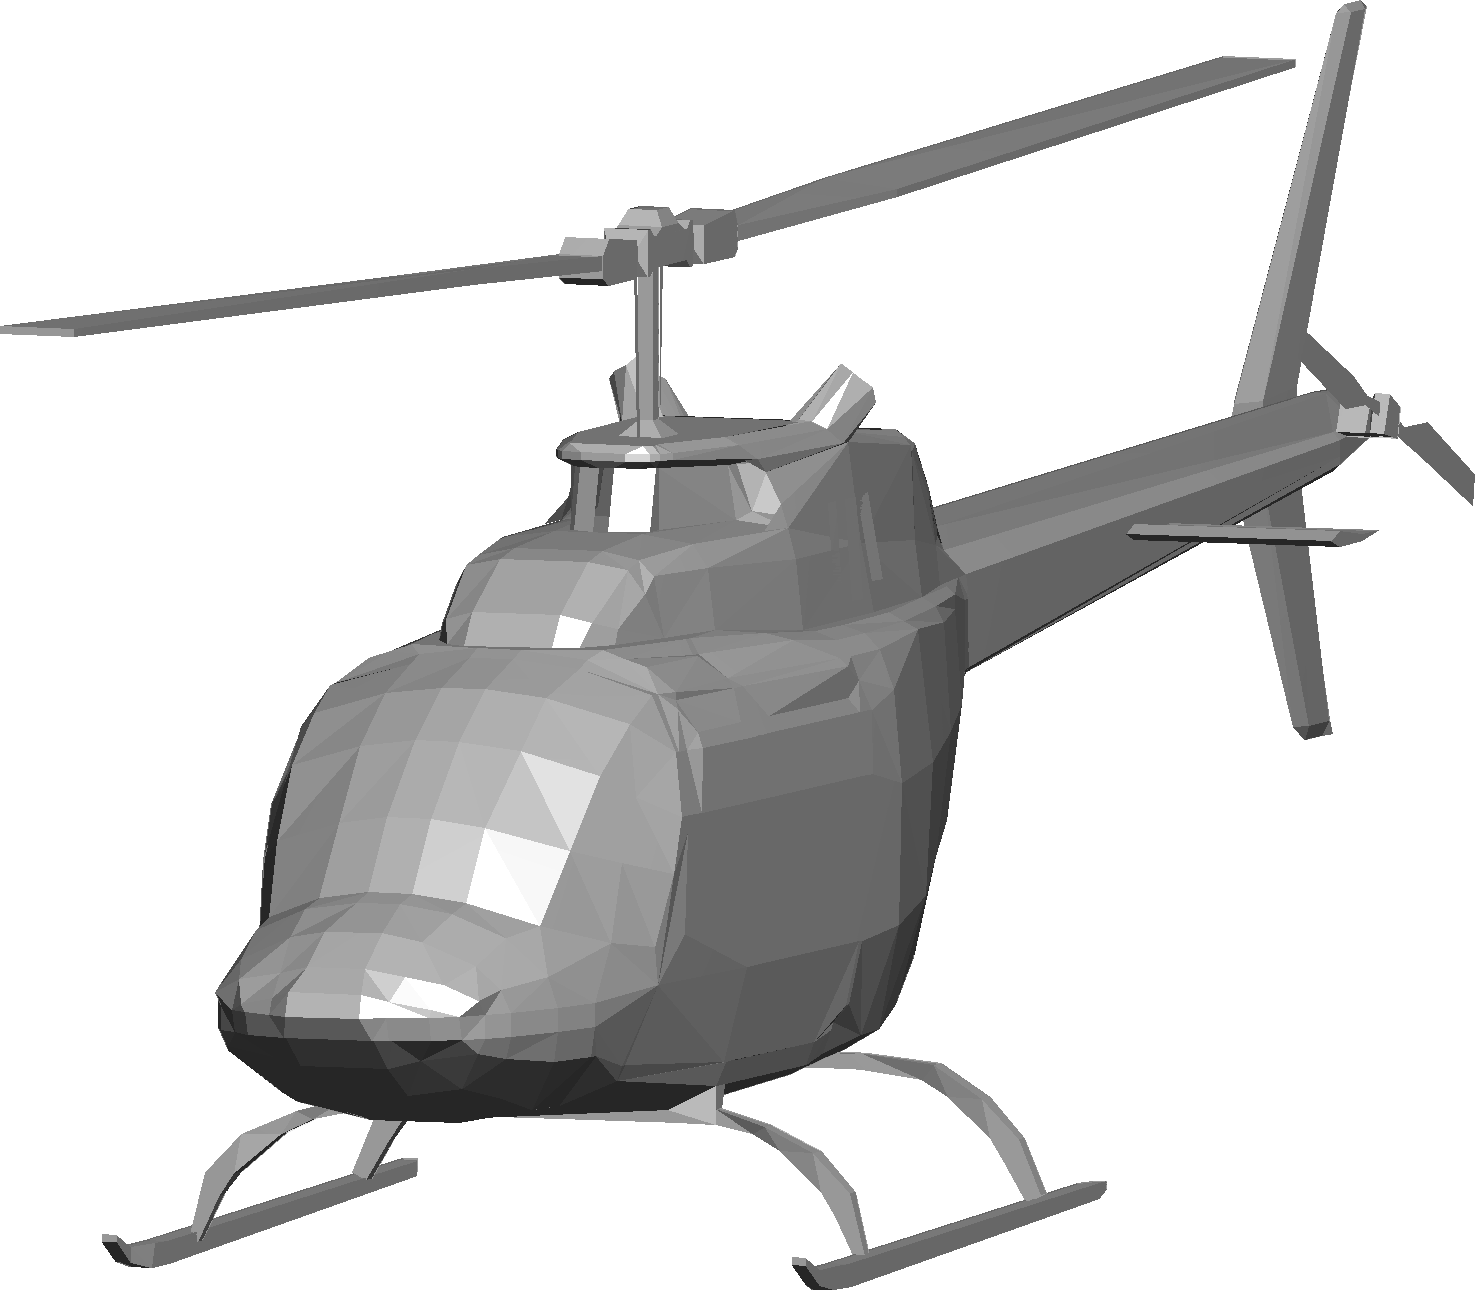
\includegraphics[width=1\linewidth]{./fig/eval/13helicopter.png}  
		\caption{Helicopter} 	
	\end{subfigure}
	\begin{subfigure}[t]{0.19\linewidth} \centering
		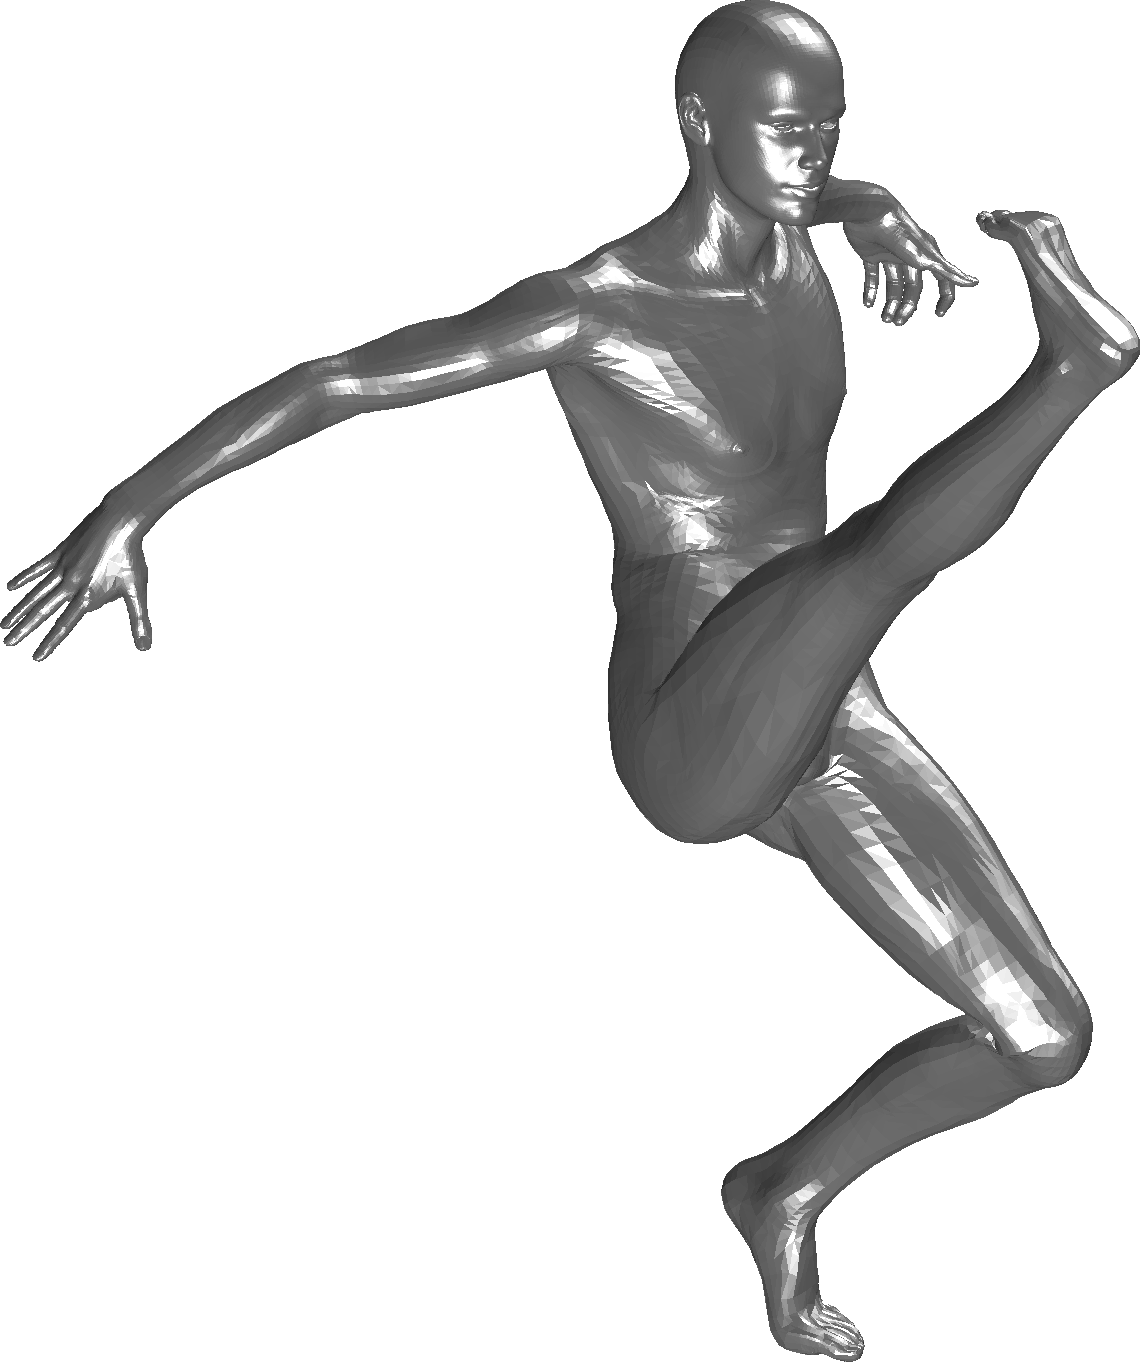
\includegraphics[width=0.8\linewidth]{./fig/eval/14man.png}  
		\caption{Kicking man} 	
	\end{subfigure} 
	\begin{subfigure}[t]{0.19\linewidth} \centering
		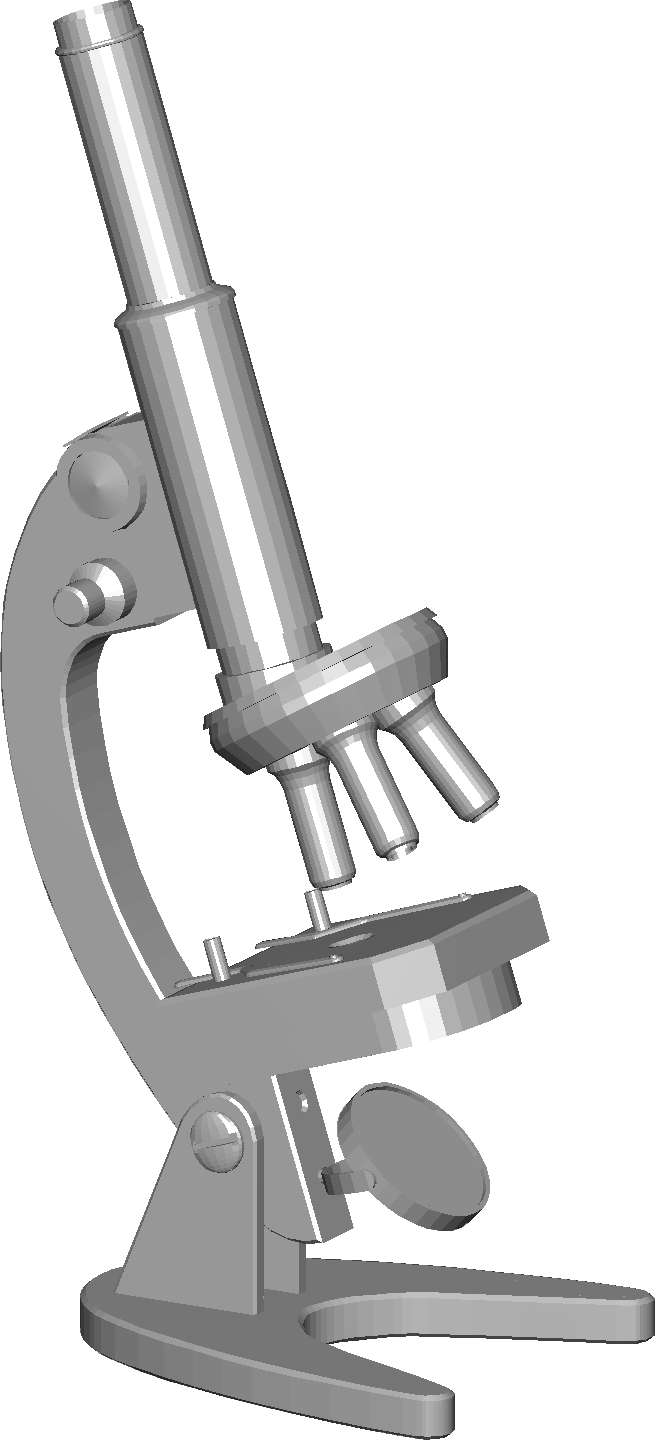
\includegraphics[width=0.5\linewidth]{./fig/eval/15microscope.png}  
		\caption{Microscope} 	
	\end{subfigure} \\ 
	\begin{subfigure}[t]{0.19\linewidth} \centering
		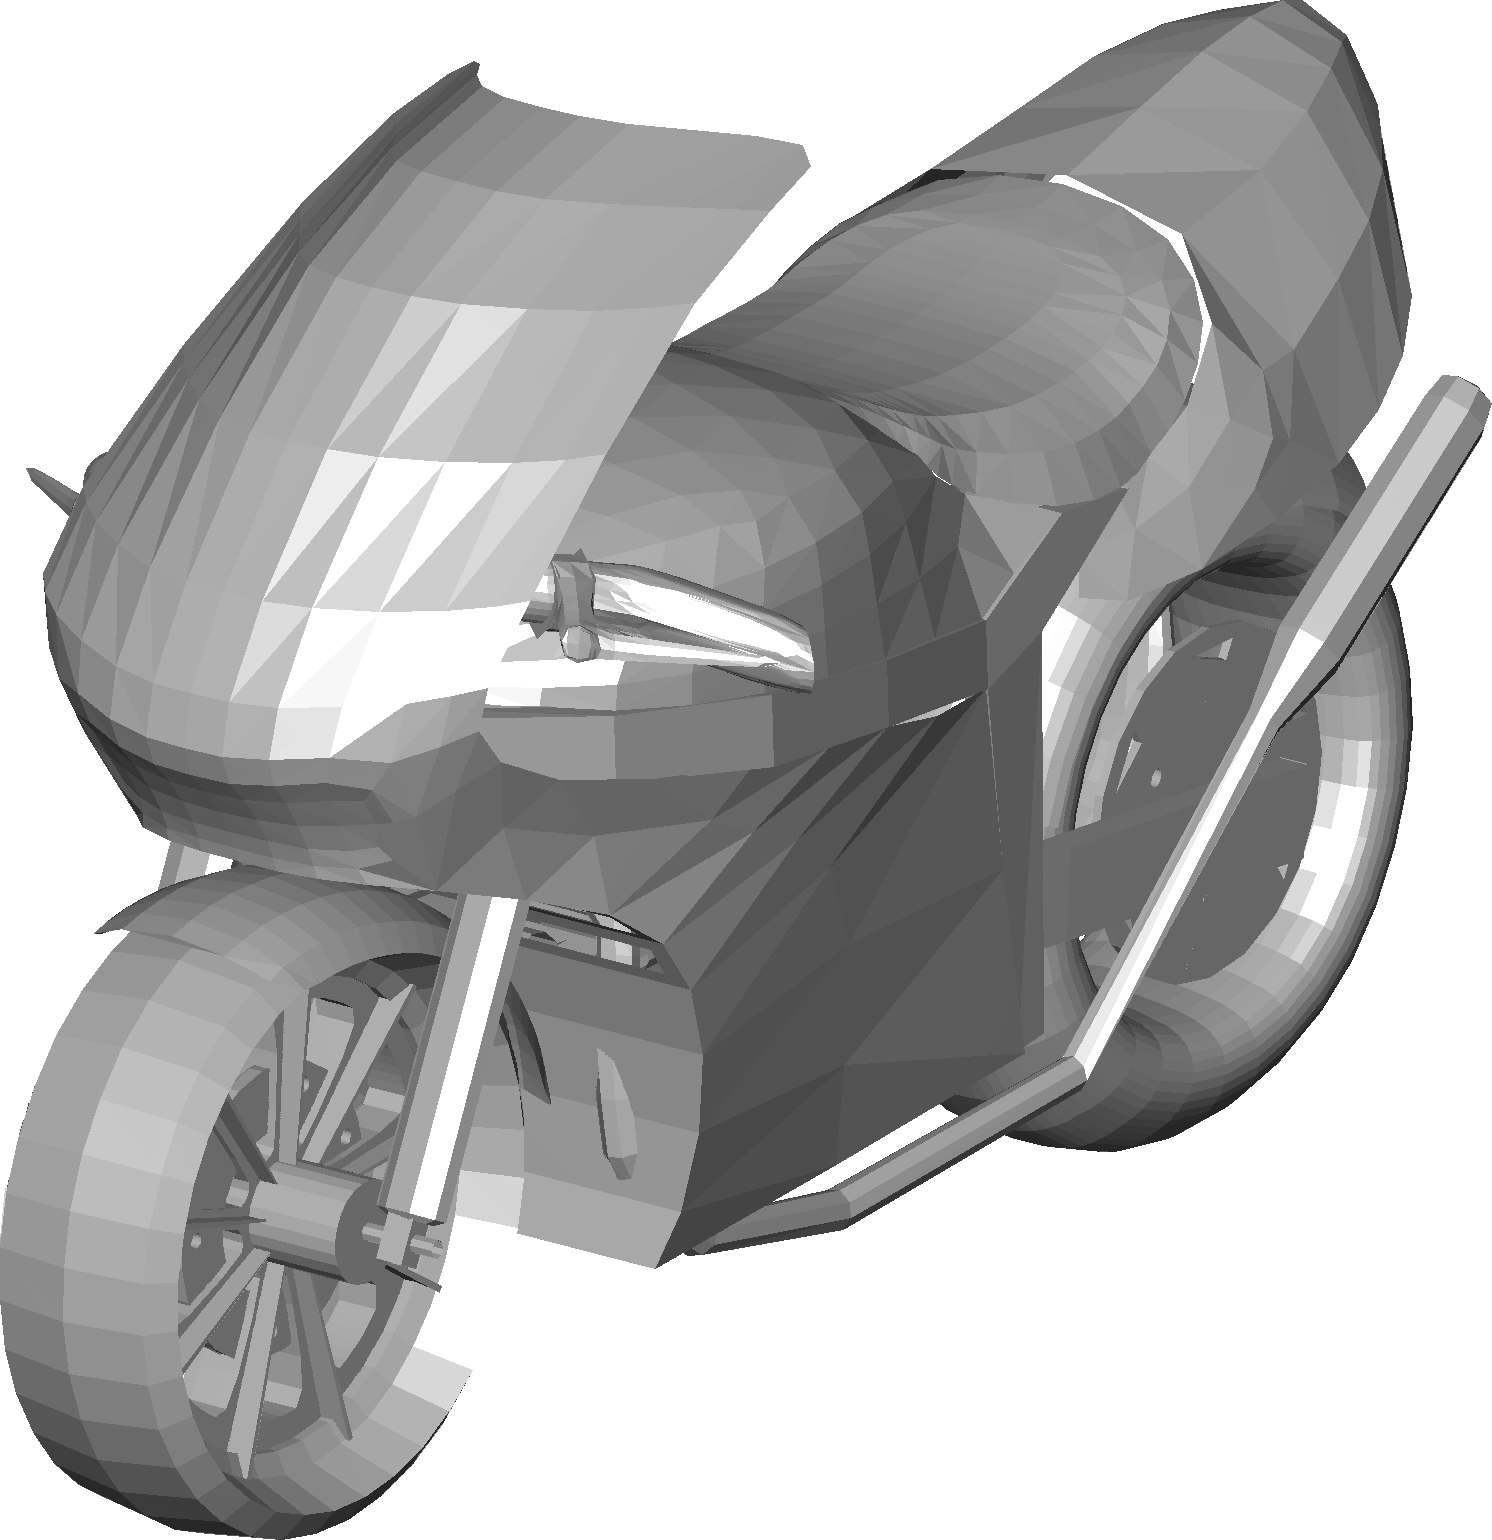
\includegraphics[width=1\linewidth]{./fig/eval/16motorbike.png}  
		\caption{Motorbike} 	
	\end{subfigure}
	\begin{subfigure}[t]{0.19\linewidth} \centering
		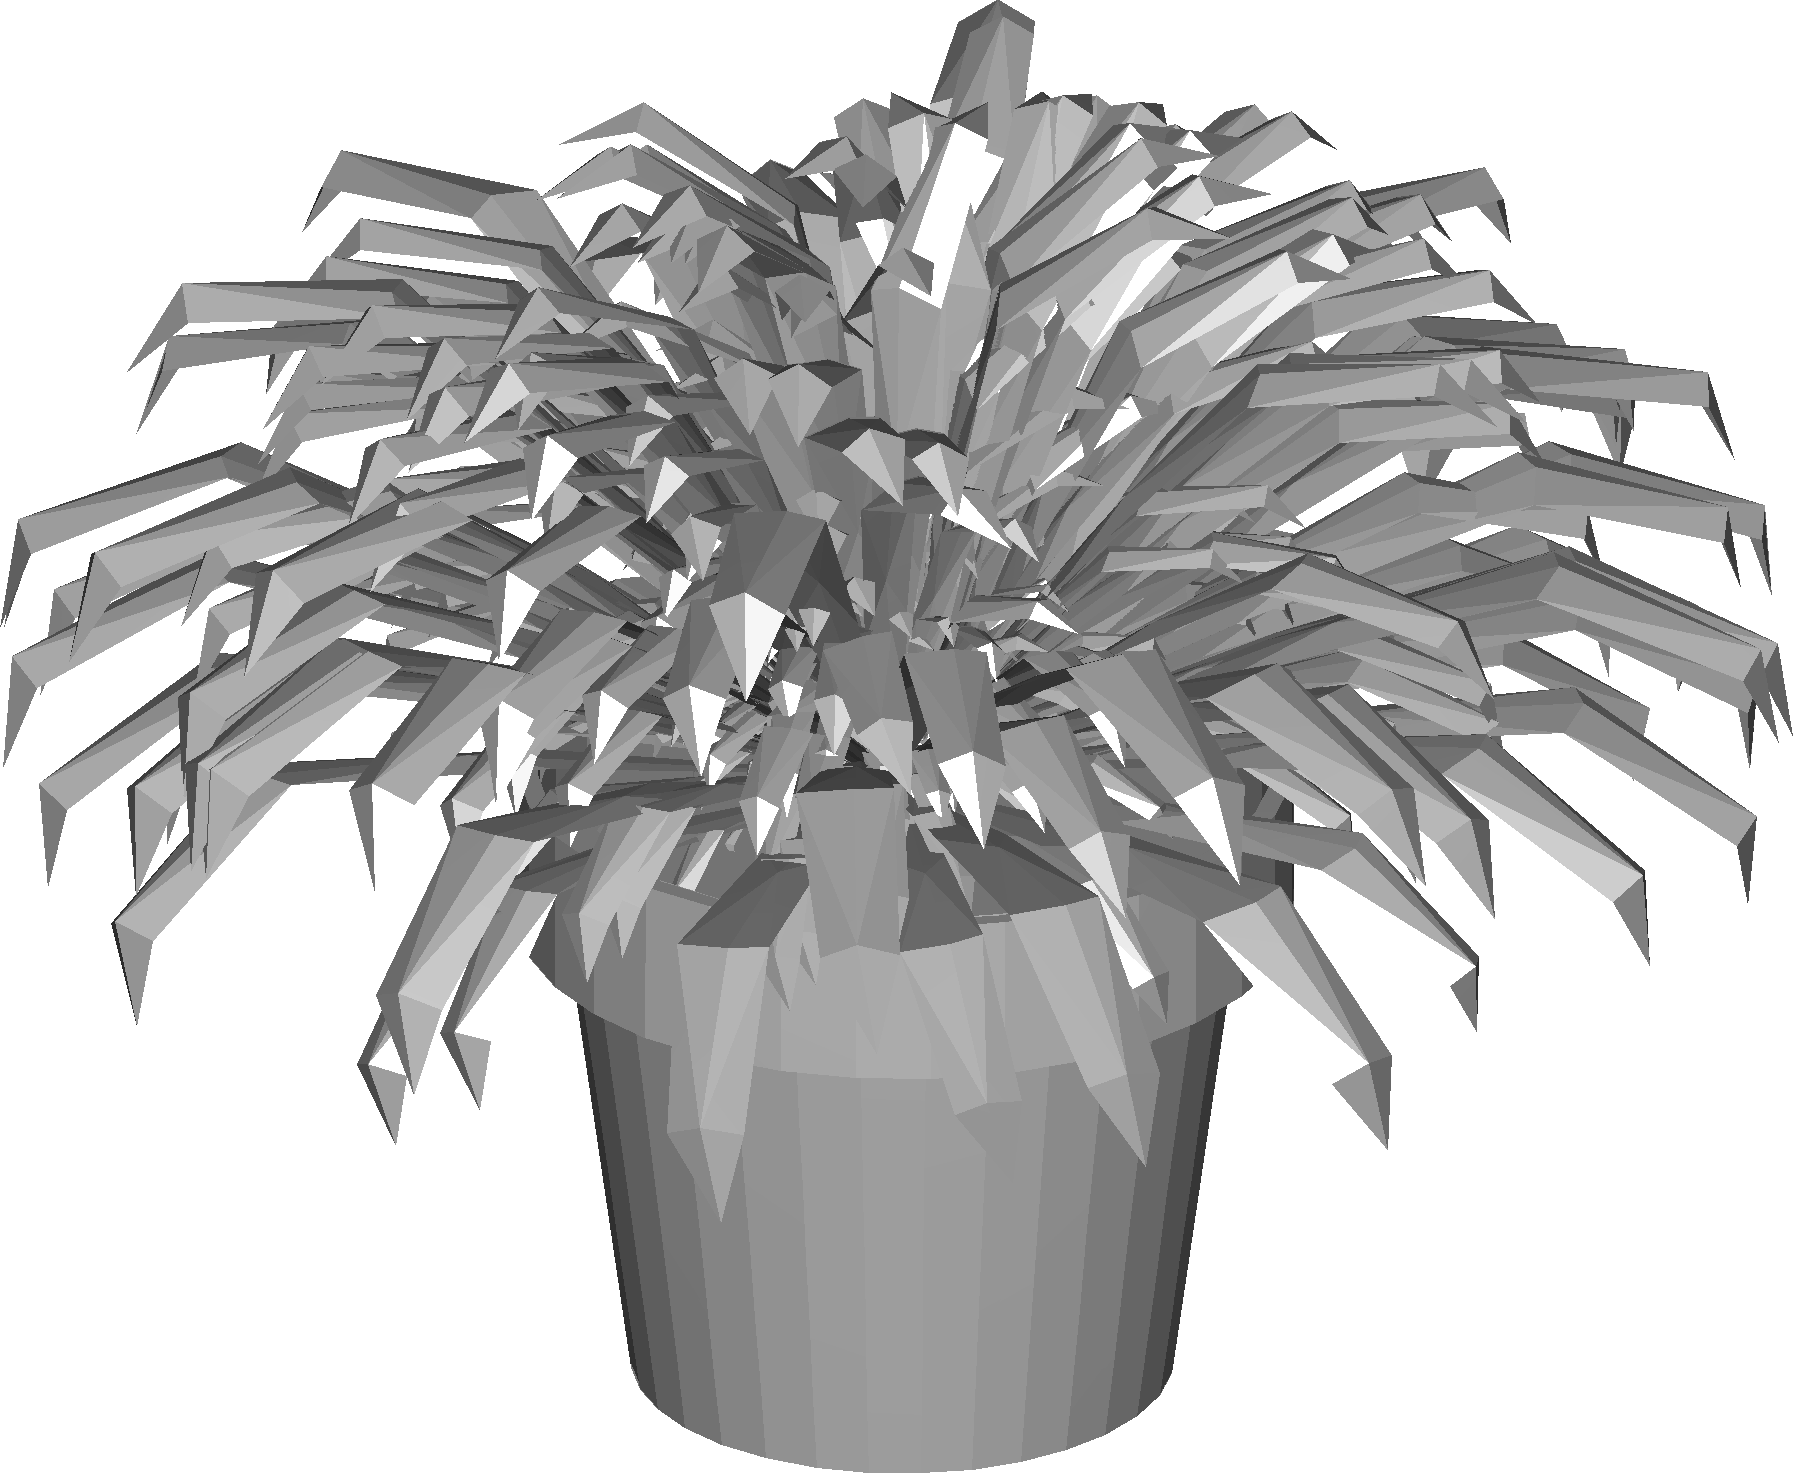
\includegraphics[width=1\linewidth]{./fig/eval/17plant.png}  
		\caption{Plant} 	
	\end{subfigure}
	\begin{subfigure}[t]{0.19\linewidth} \centering
		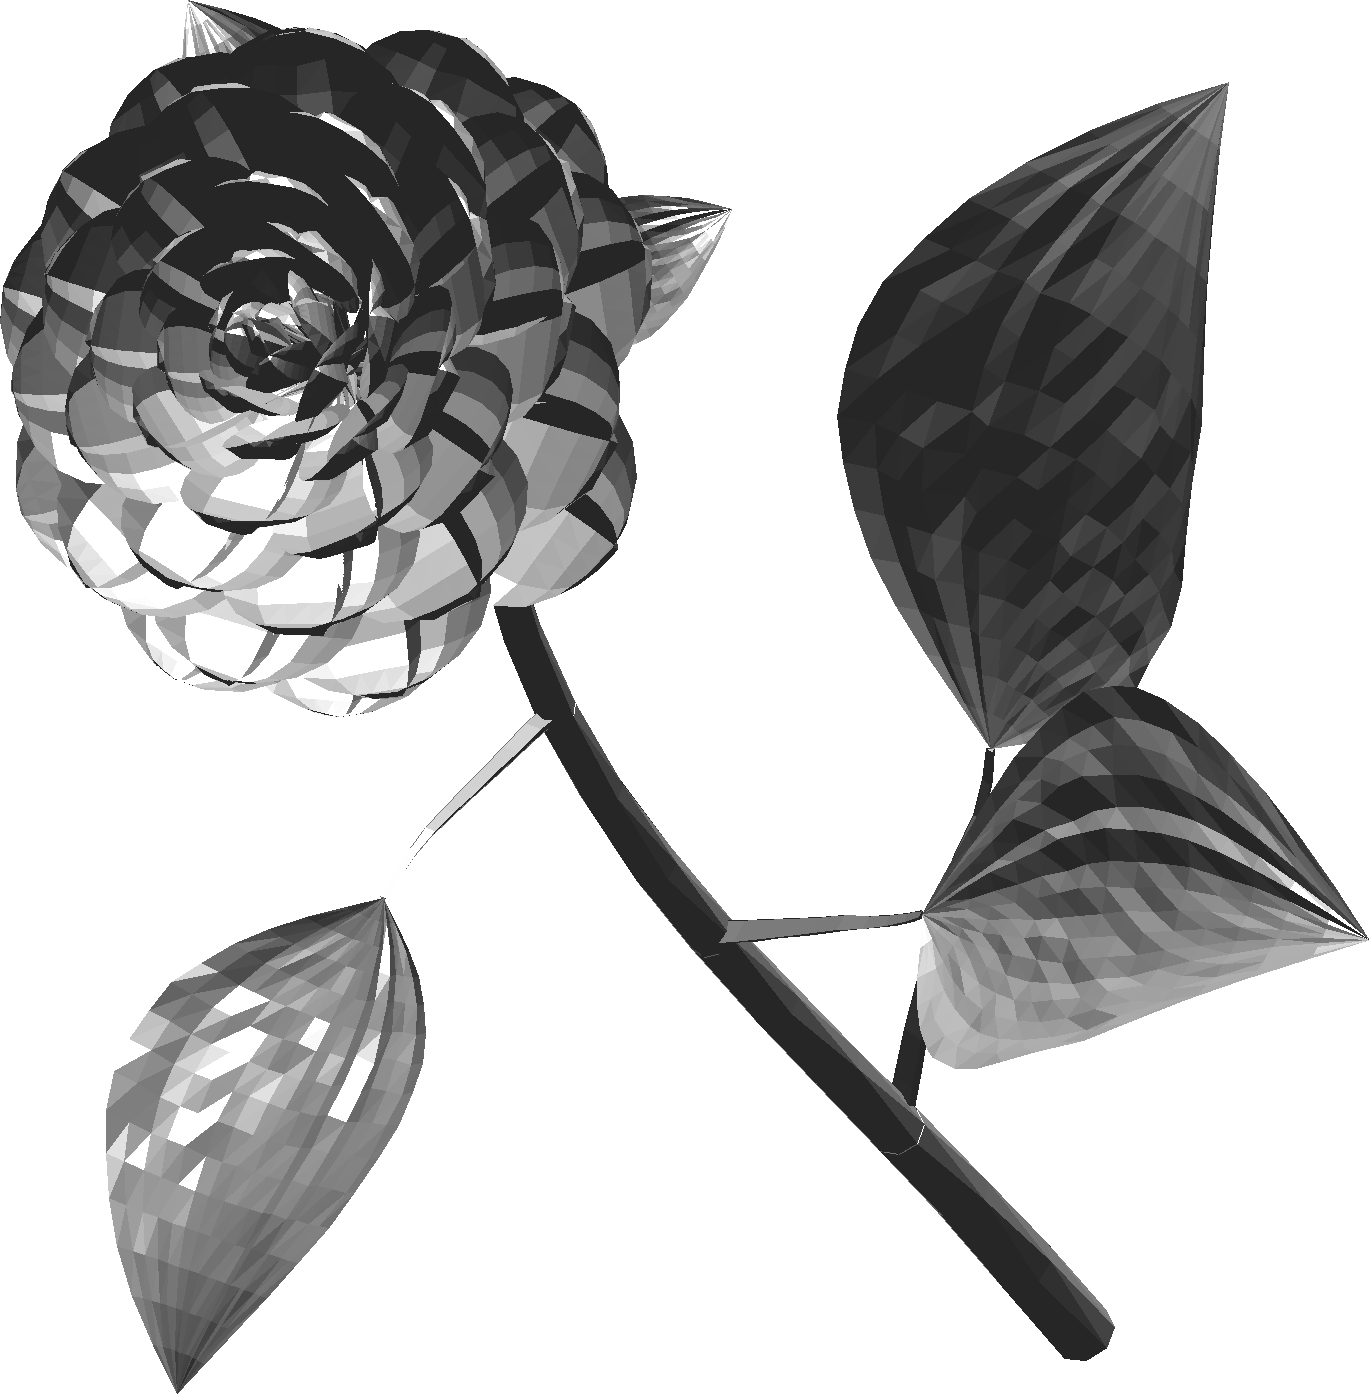
\includegraphics[width=1\linewidth]{./fig/eval/18rose.png}  
		\caption{Rose} 	
	\end{subfigure}
	\begin{subfigure}[t]{0.19\linewidth} \centering
		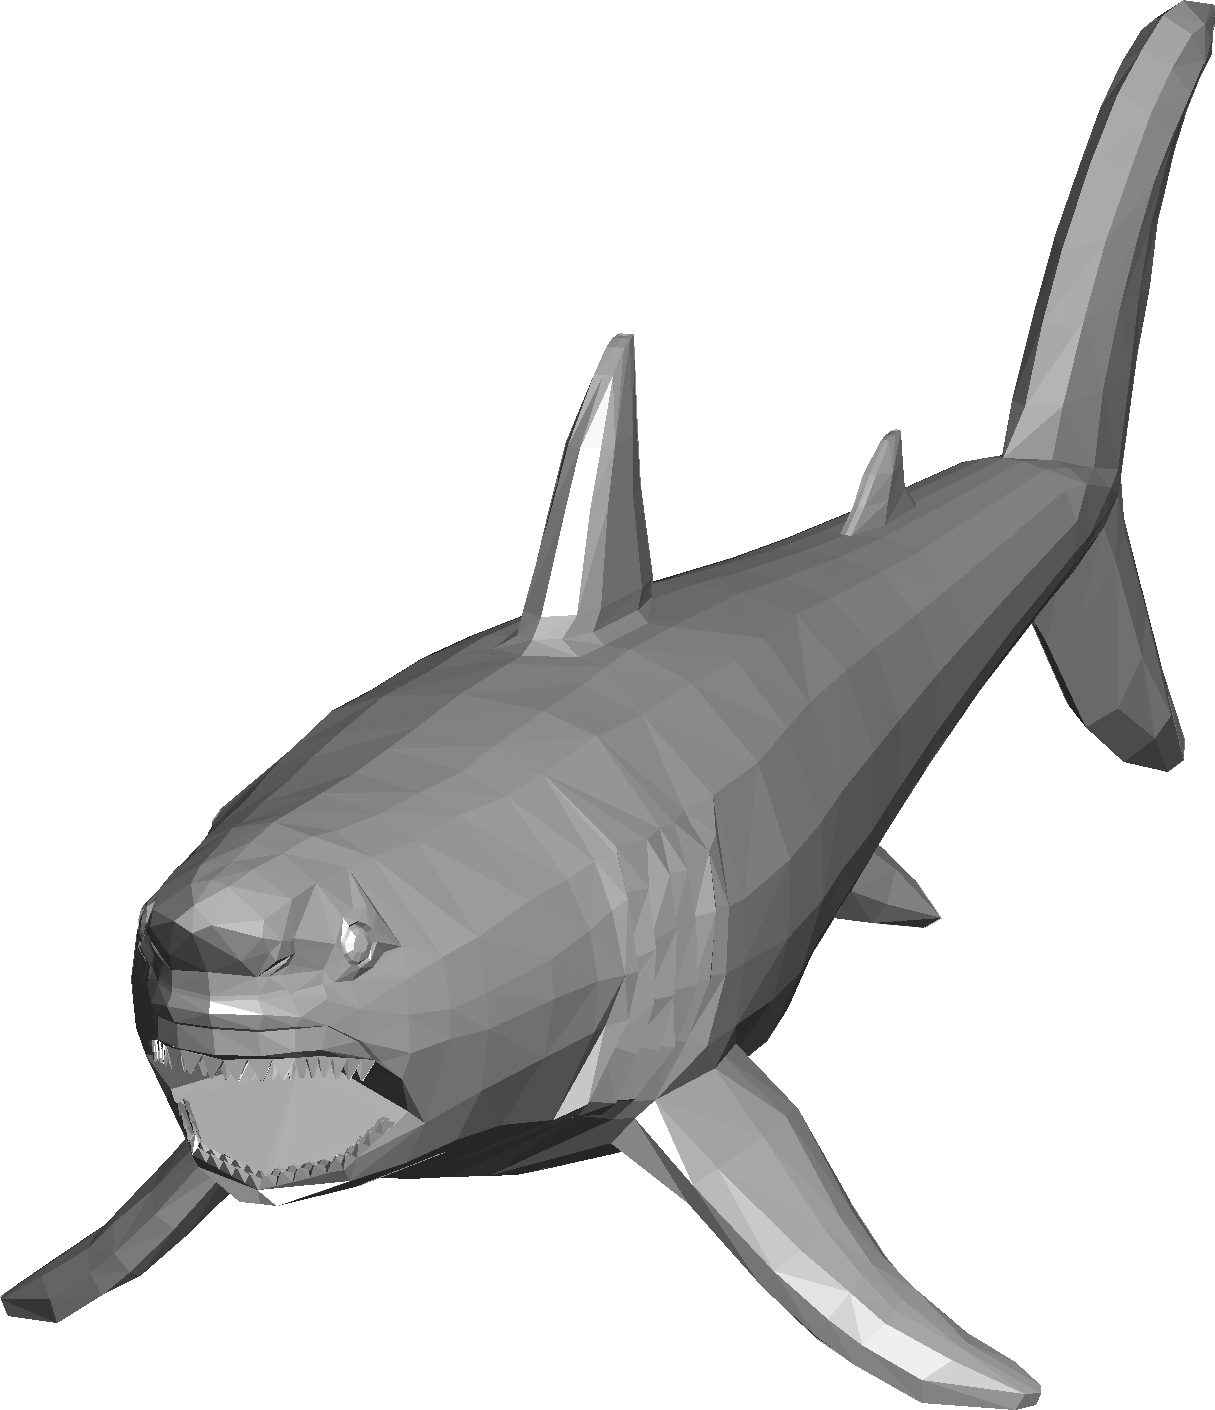
\includegraphics[width=1\linewidth]{./fig/eval/19shark.png}  
		\caption{Shark} 	
	\end{subfigure} 
	\begin{subfigure}[t]{0.19\linewidth} \centering
		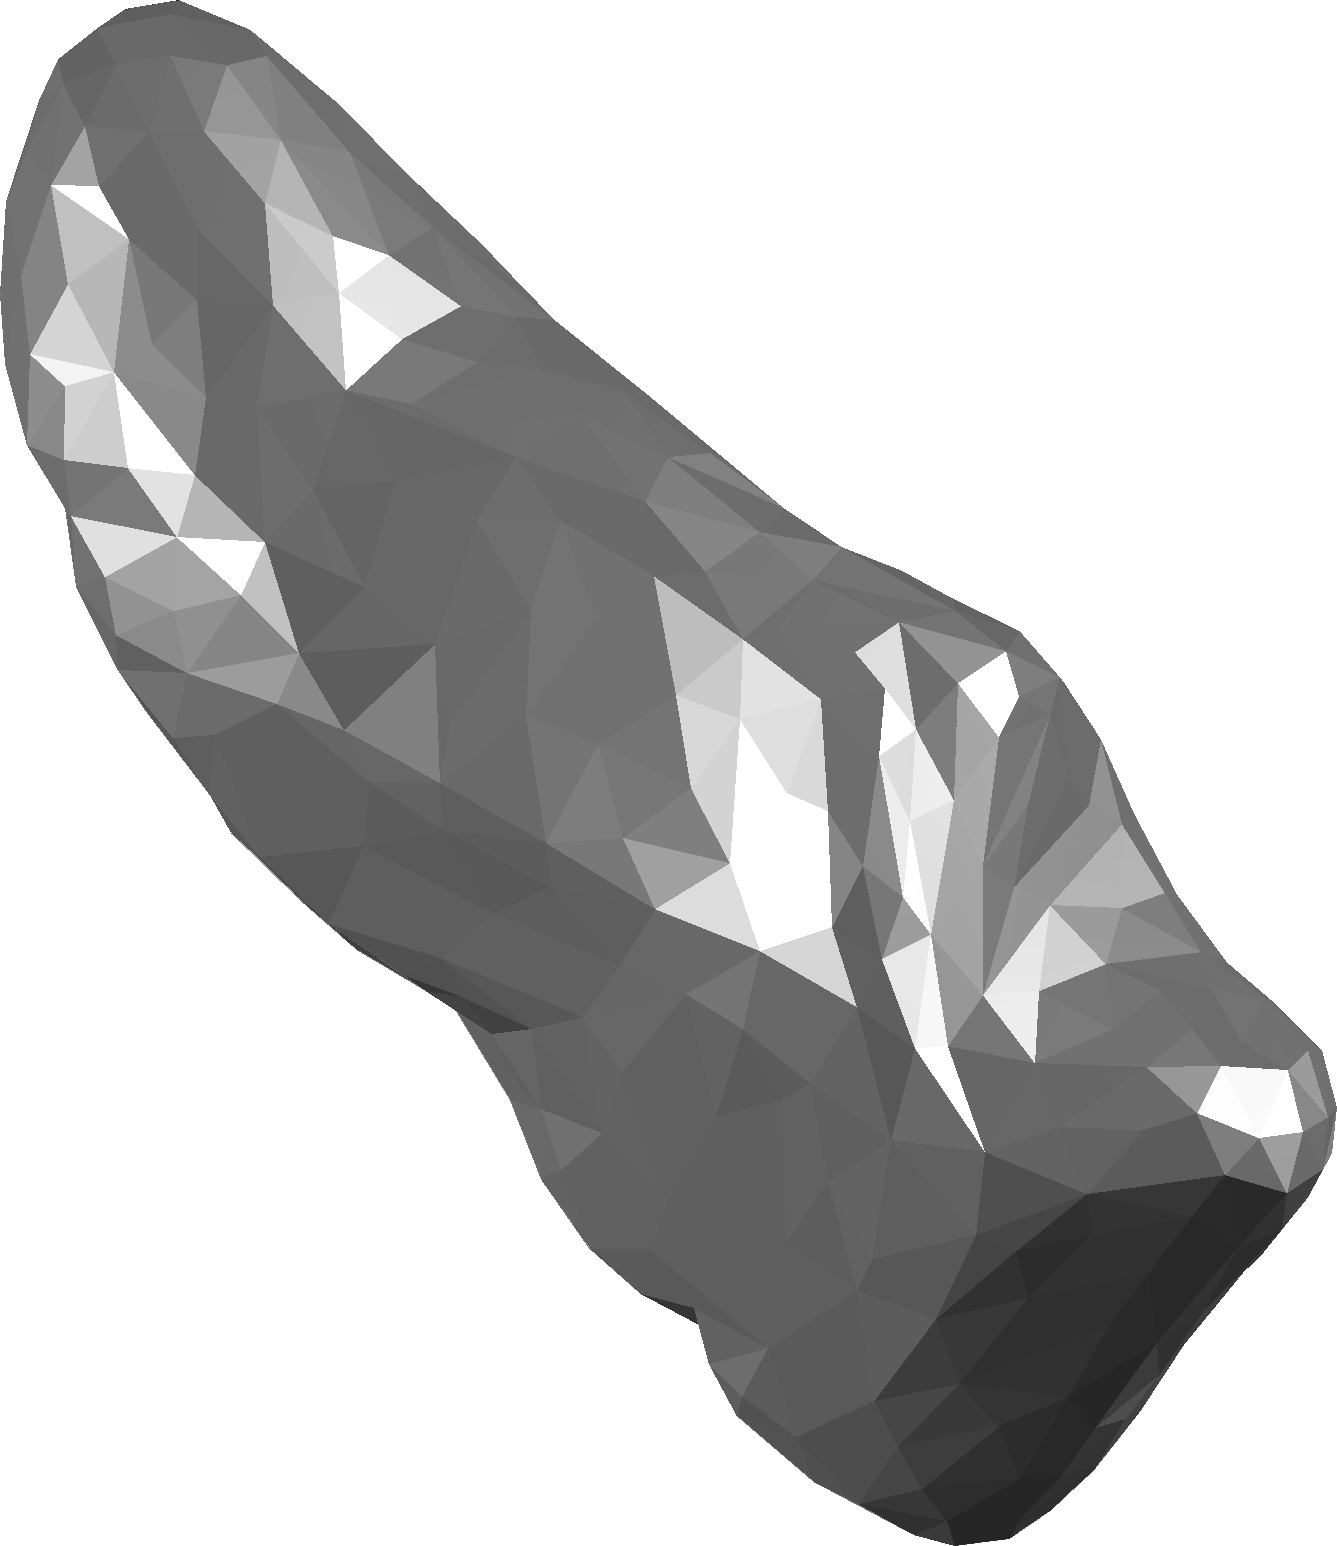
\includegraphics[width=1\linewidth]{./fig/eval/20shoe.png}  
		\caption{Shoe} 	
	\end{subfigure} \\ 
	\begin{subfigure}[t]{0.19\linewidth} \centering
		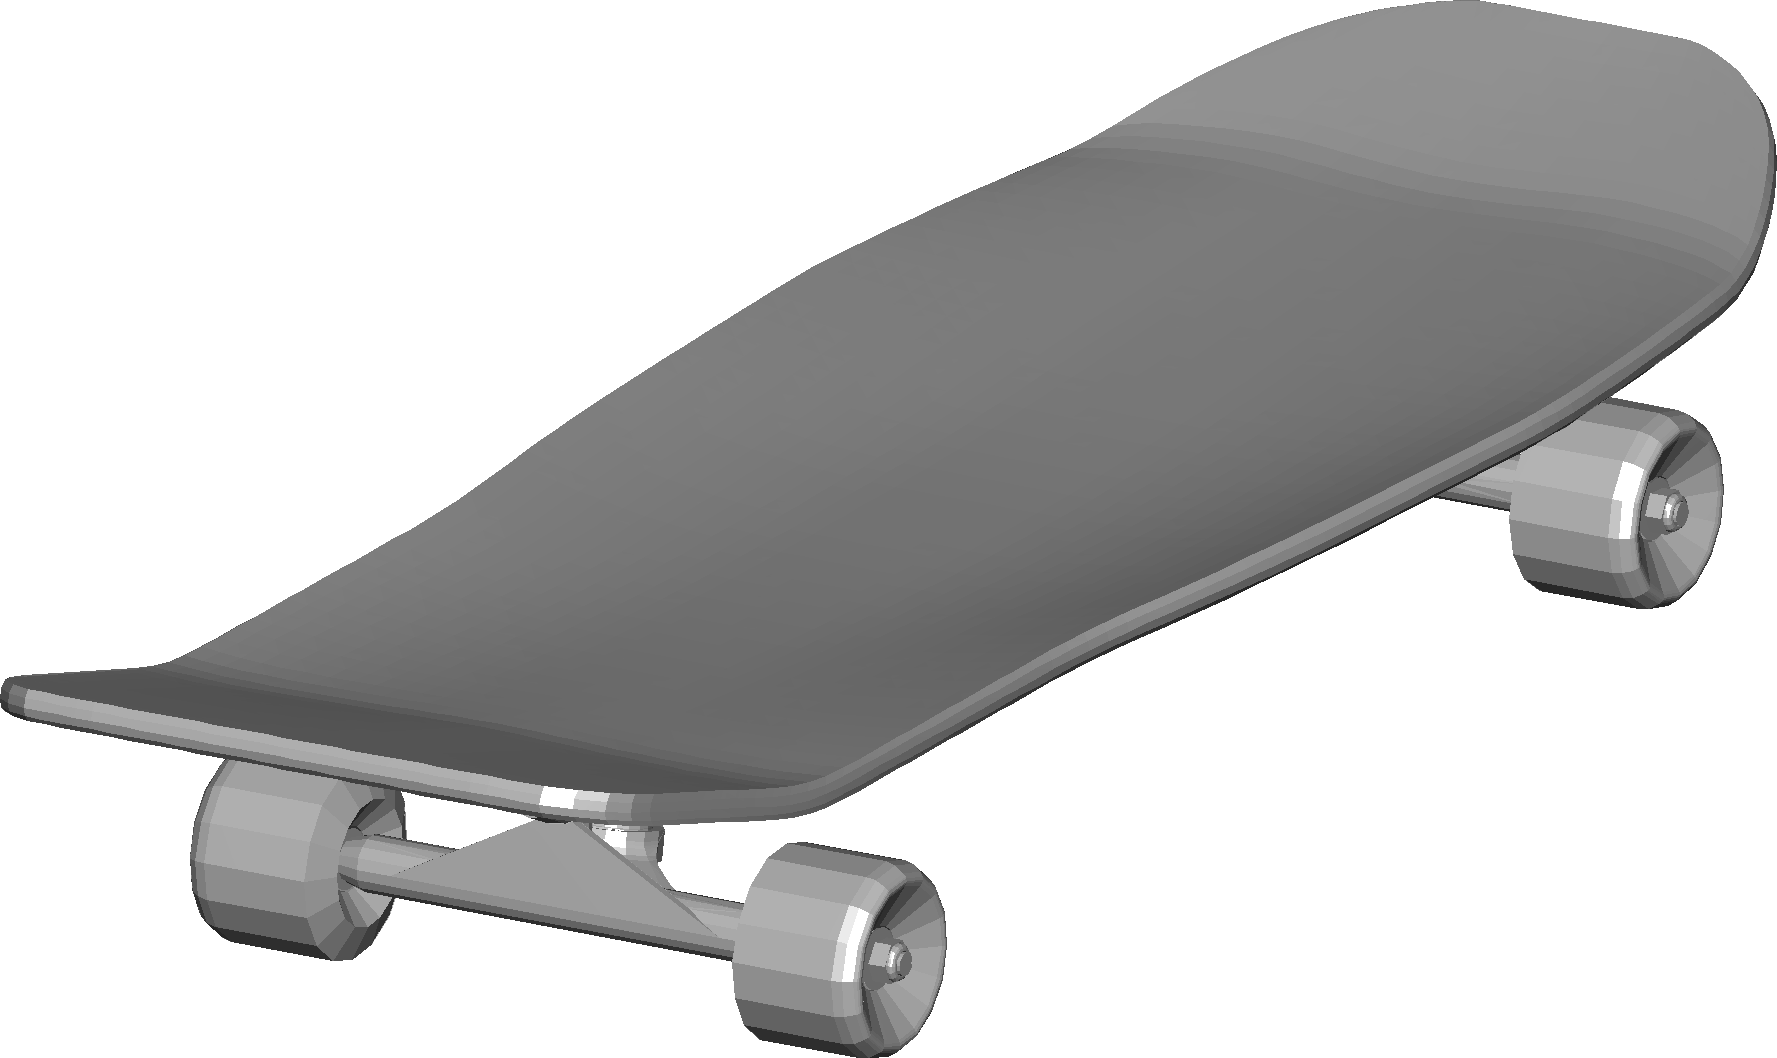
\includegraphics[width=1\linewidth]{./fig/eval/21skateboard.png}  
		\caption{Skateboard} 	
	\end{subfigure}
	\begin{subfigure}[t]{0.19\linewidth} \centering
		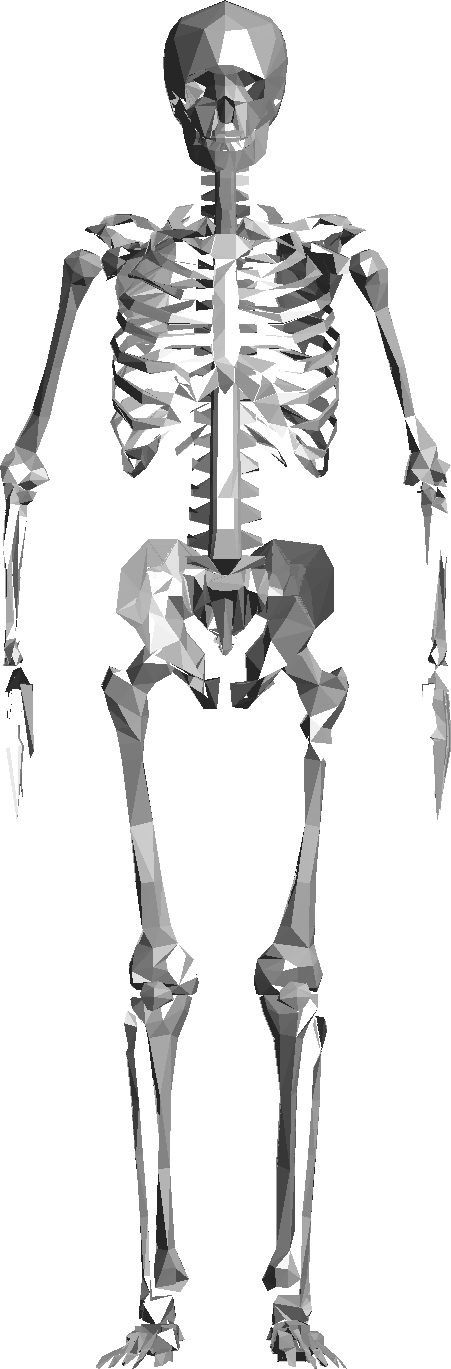
\includegraphics[width=0.3\linewidth]{./fig/eval/22skeleton.png}  
		\caption{Skeleton} 	
	\end{subfigure}
	\begin{subfigure}[t]{0.19\linewidth} \centering
		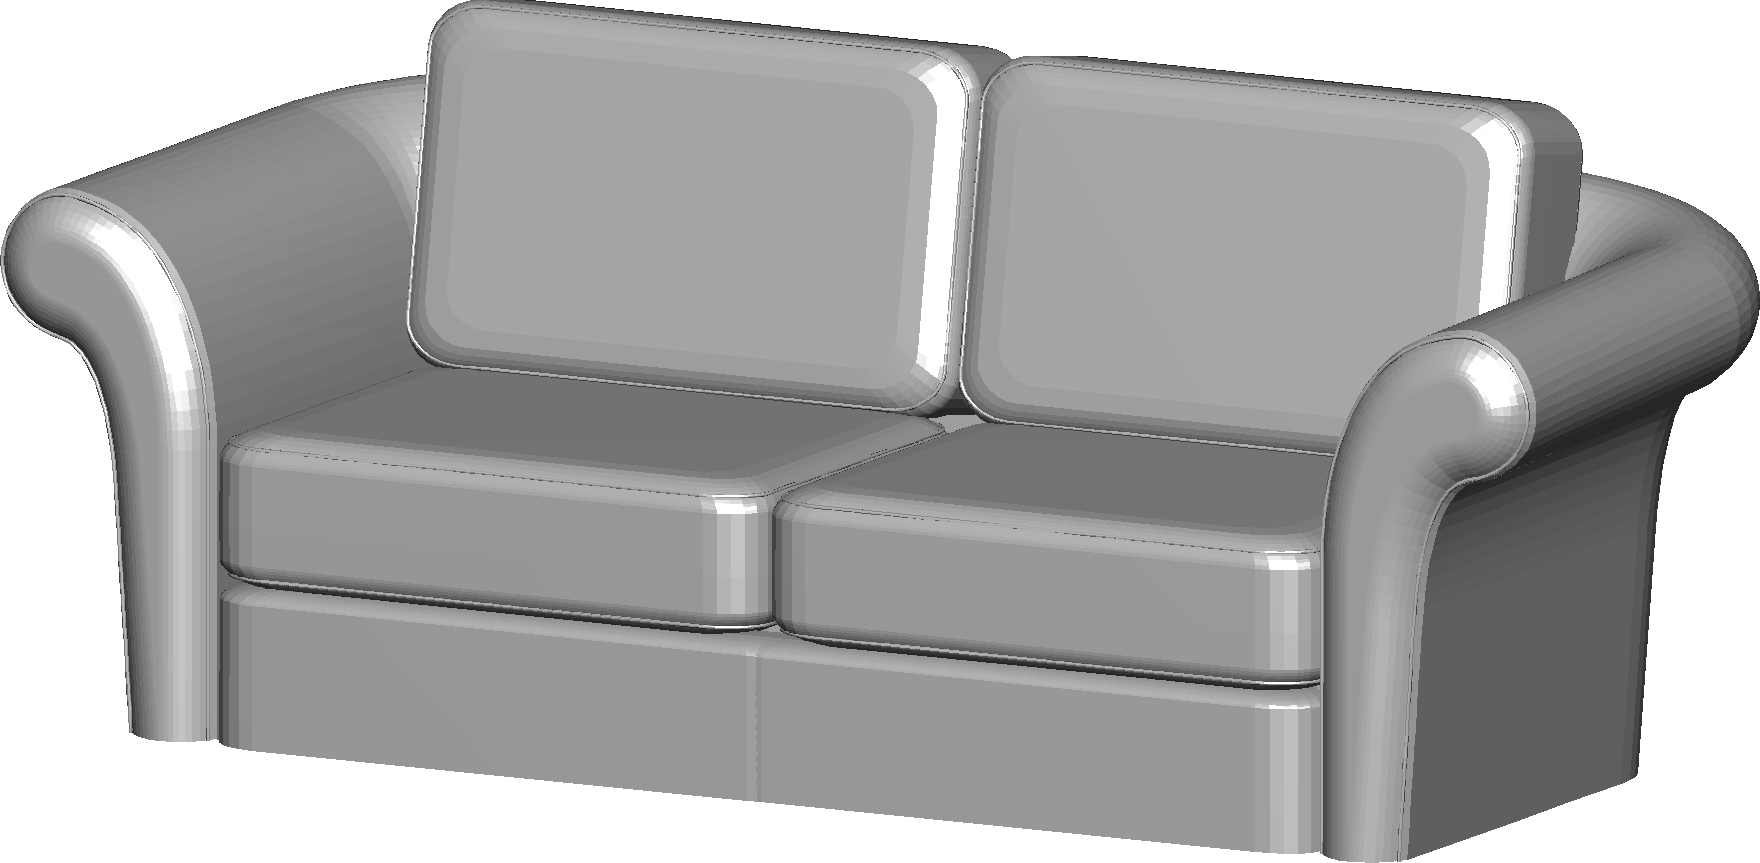
\includegraphics[width=1\linewidth]{./fig/eval/23sofa.png}  
		\caption{Sofa} 	
	\end{subfigure}
	\begin{subfigure}[t]{0.19\linewidth} \centering
		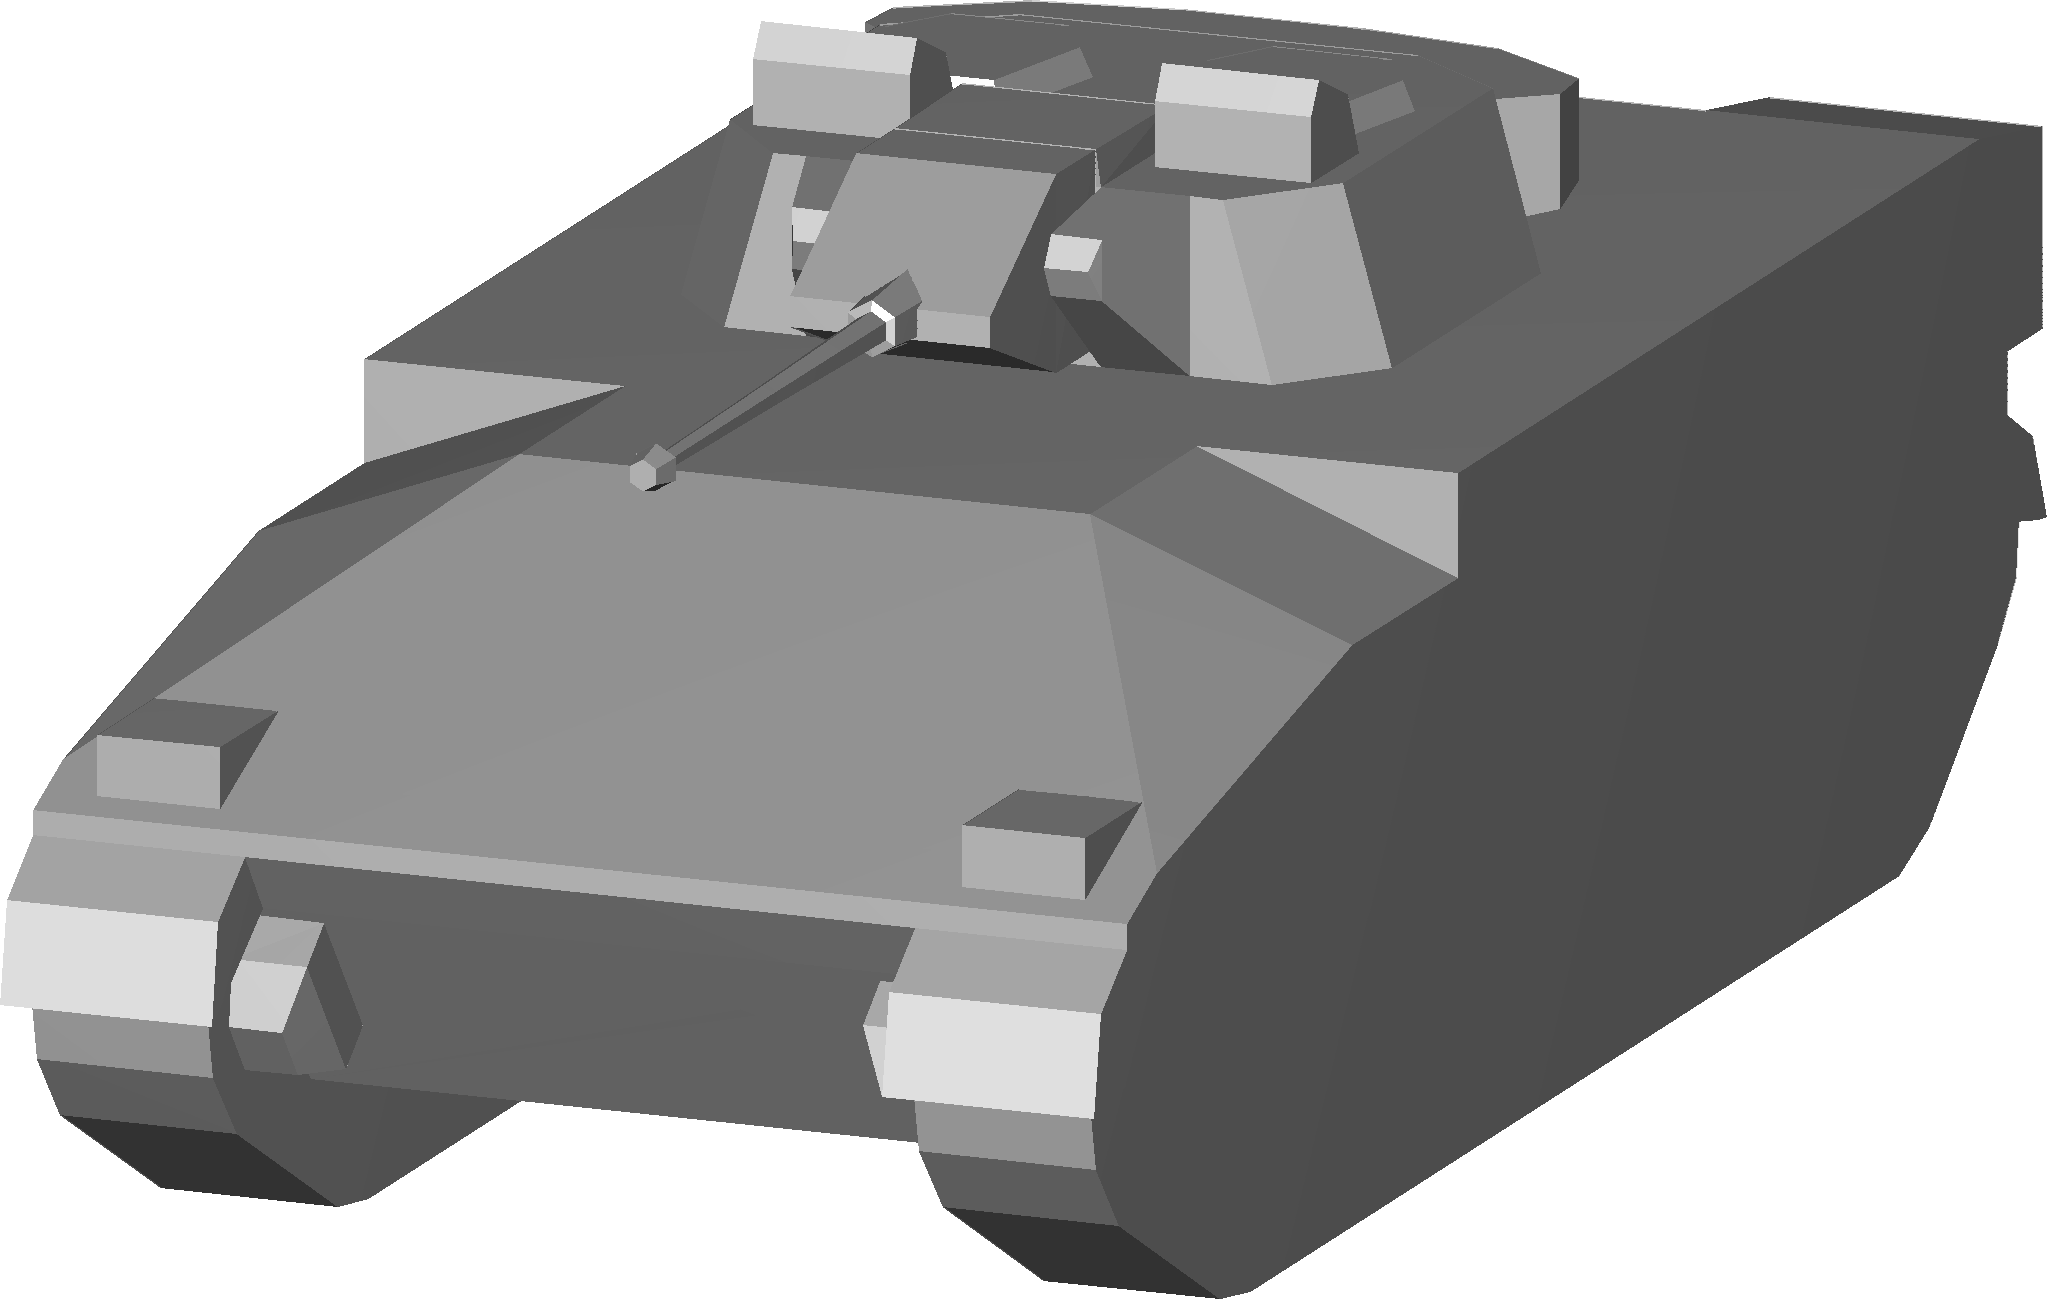
\includegraphics[width=1\linewidth]{./fig/eval/24tank.png}  
		\caption{Tank} 	
	\end{subfigure} 
	\begin{subfigure}[t]{0.19\linewidth} \centering
		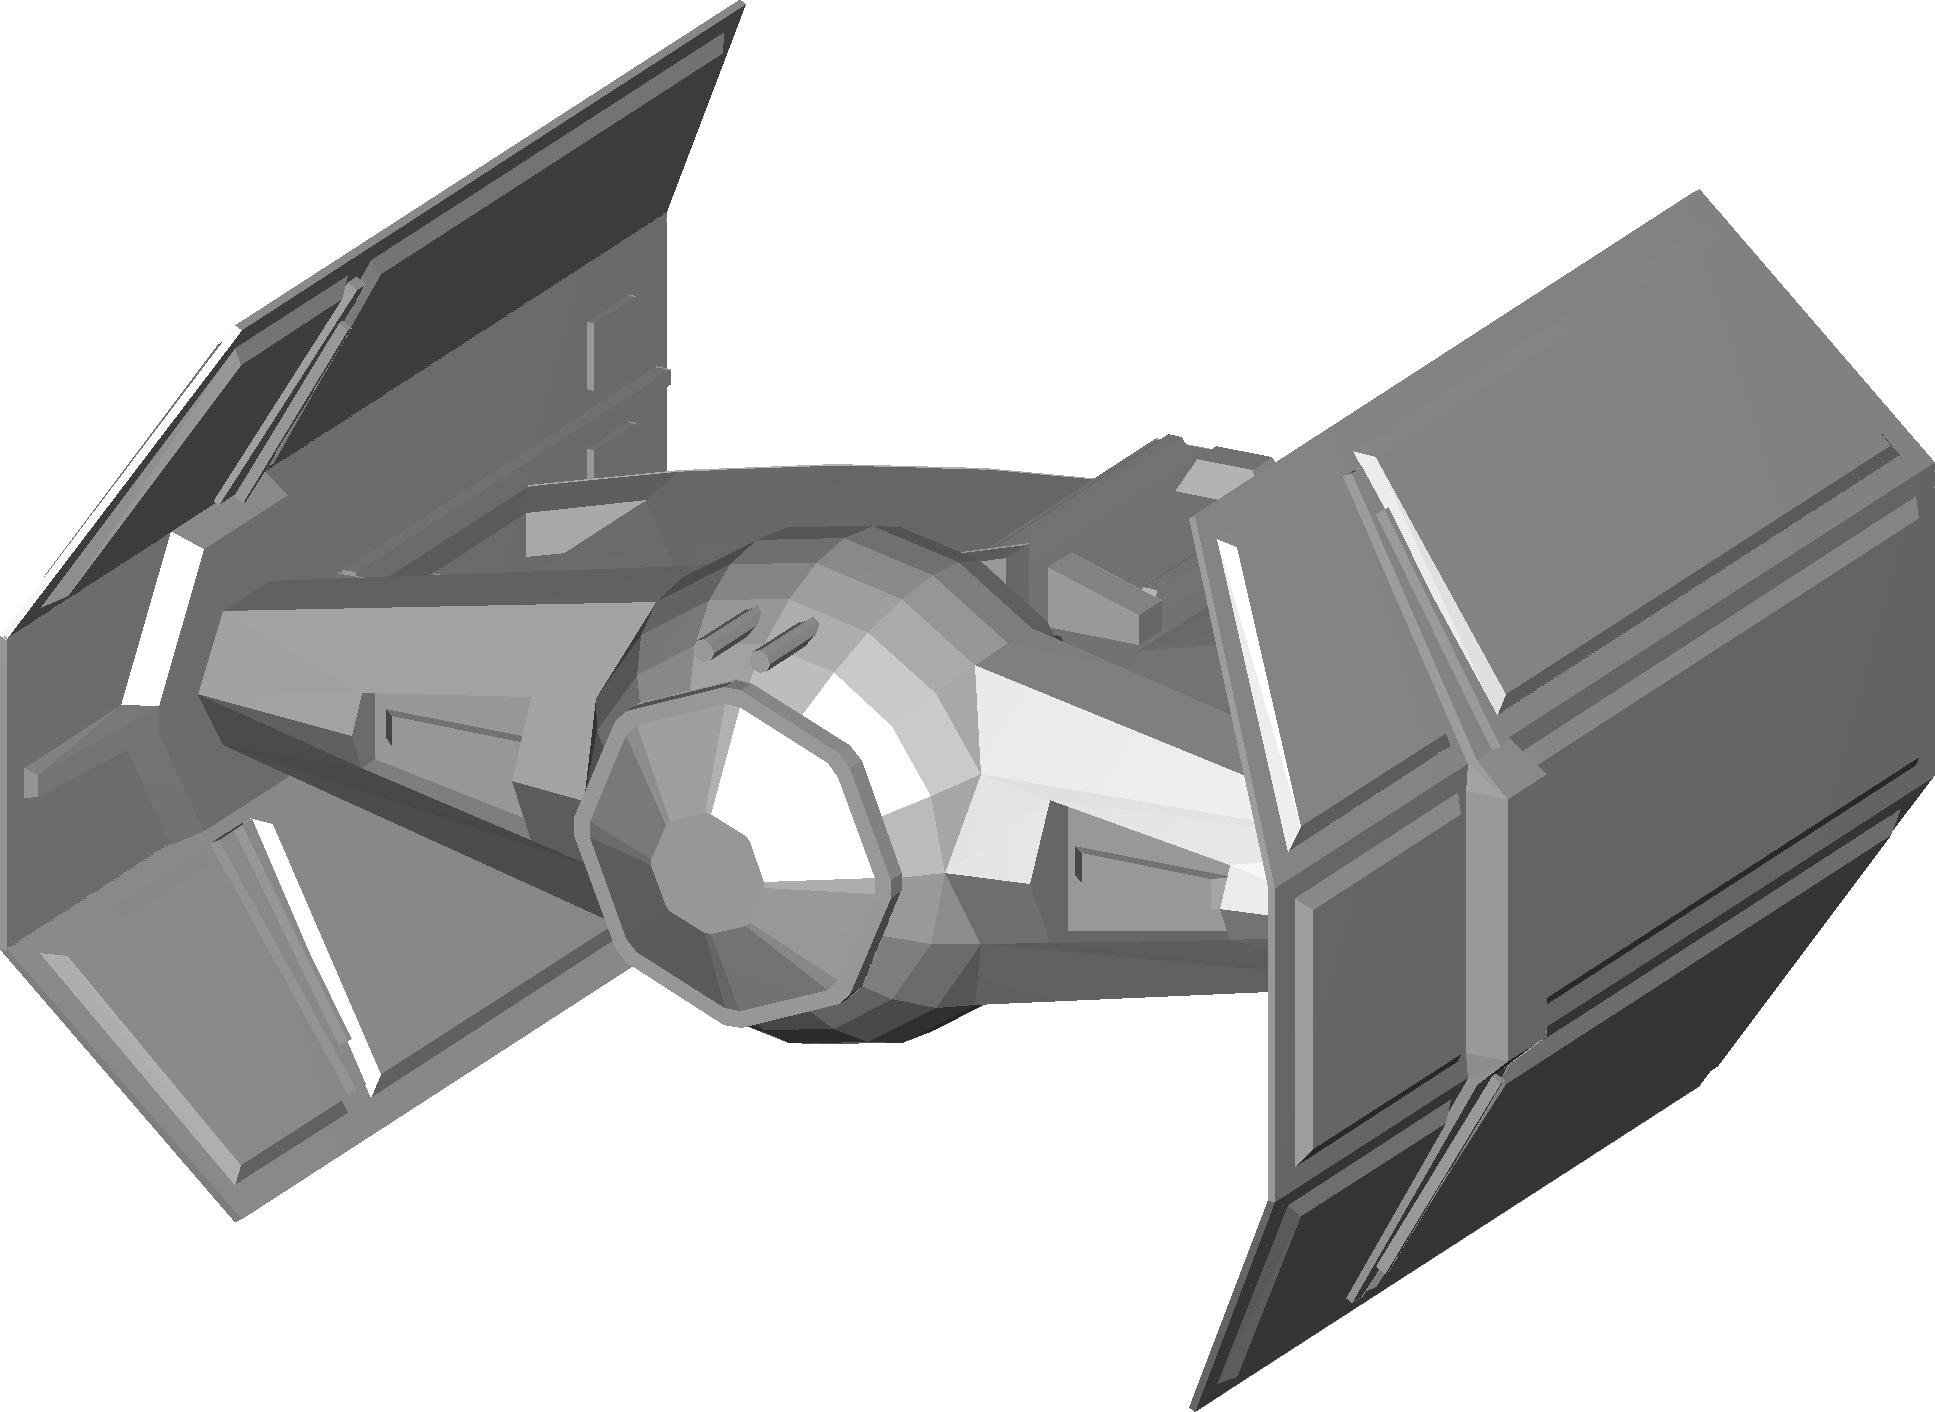
\includegraphics[width=1\linewidth]{./fig/eval/25tiefighter.png}  
		\caption{Tiefighter} 	
	\end{subfigure} 
	\caption{The sample 3D shapes in the \meshset dataset.}
	\label{fig/eval/sampleshapes}
\end{figure}


\subsection{Experimental setup}
\label{sec/eval/variation}
% done 
In the evaluation experiments, a series of transformed shapes were created from the reference shape with different magnitudes of a test parameter. A repeatability score was computed by matching the two sets of interest points to each other, according to equation \ref{eqn/eval/rptarea}. The overall performance of one dataset was measured by averaging the $\areascore$ scores across all shapes in the evaluation dataset. 

% done 
The characteristics of the interest point detectors were evaluated under five different variations. These include (1) rotation, (2) translation, (3) scale, (4) sampling density and (5) sampling noise. 
For \mriset and \stereoset, such variations were introduced during the process of shape acquisition. Shapes in the \meshset dataset can be generated synthetically with different variations.

% done 
The variations and parameters used in the evaluation datasets were described in table \ref{tab/eval/datavar}. Although image compression rate and lighting change were also evaluated for image-based detectors \cite{Mikolajczyk2005}, similar experiments were not necessary for 3D shape data because they were unaffected by such factors. 

% done 
\begin{table}[ht]
\centering
\begin{tabular}{cc|ccccc}
\hline
\multirow{2}{*}{ } & \multirow{2}{*}{ } & \multicolumn{5}{c}{\textbf{Variations}} \\ \cline{3-7} 
& & \textbf{Noise} & \textbf{Density} & \textbf{Scale} & \textbf{Rotation} & \textbf{Translation} \\
\hline
\multirow{3}{*}{\textbf{Dataset}} & \meshset & \checkmark & \checkmark & \checkmark & \checkmark & \\
& \mriset & \checkmark & & & \checkmark & \checkmark \\
& \stereoset & \checkmark & \checkmark & \checkmark & \checkmark & \checkmark \\
\hline
\end{tabular}
\caption{Variations observed in the evaluation datasets}
\label{tab/eval/datavar}
\end{table}

Performances of the candidate detectors were measured as each test parameter was varied individually, keeping all the other parameters at their default values. Sampling-related parameters (\ie noise level and sampling density) were applied to all shape instances, whilst pose parameters (\ie rotation, translation and scale) were applied to only one instance in each matching pair. Some parameters were defined in terms of $L$, which was the largest dimension of the voxelised reference shapes. The voxelisation process limited the maximum value of $L$ to $200$ voxels. The default parameters for the reference shapes, and the number of transformed shapes created for matching, are summarised in table \ref{tab/eval/referenceparam}. 

\begin{table}[ht]
\centering
\begin{tabular}{c|c}
\hline
\multicolumn{2}{c}{ \textbf{Default parameters for reference shapes }} \\ 
\hline 
\textbf{Parameter} & \textbf{Value} \\
\hline
Default point cloud size & $50000$ points\\
Default noise $\sigma_{n}$ & $0.0025L$\\ 
Default rotation & $0^{\circ}$\\
Maximum $L$ & $200$ voxels\\
Default $\sigma_{\textrm{KDE}}$ in $g(\cdot,\sigma_{\textrm{KDE}})$ & $1.5$ voxels \\ 
Distance threshold $\disp$ & $0.03L$ \\
Parameter $f$ in equation (\ref{eqn/eval/loc_vec}) & $\sqrt{8}$ \\
Number of octaves in scale-space & $4$ \\
\hline
\multicolumn{2}{c}{ \textbf{ Number of transformed shapes compared }} \\
\hline 
\textbf{Parameter} & \textbf{Value} \\
\hline
Sampling noise & 13 \\
Sampling density & 17 \\
Noise & 21 \\
Scale & 21 \\
\hline
\end{tabular}
\caption{The reference parameters for the testing shapes}
\label{tab/eval/referenceparam}
\end{table}

\subsection{Experiments on synthetic meshes}

\subsubsection{Sampling noise}

% done
\begin{figure}[ht]
	\centering
	\begin{subfigure}[t]{0.24\linewidth}\centering
		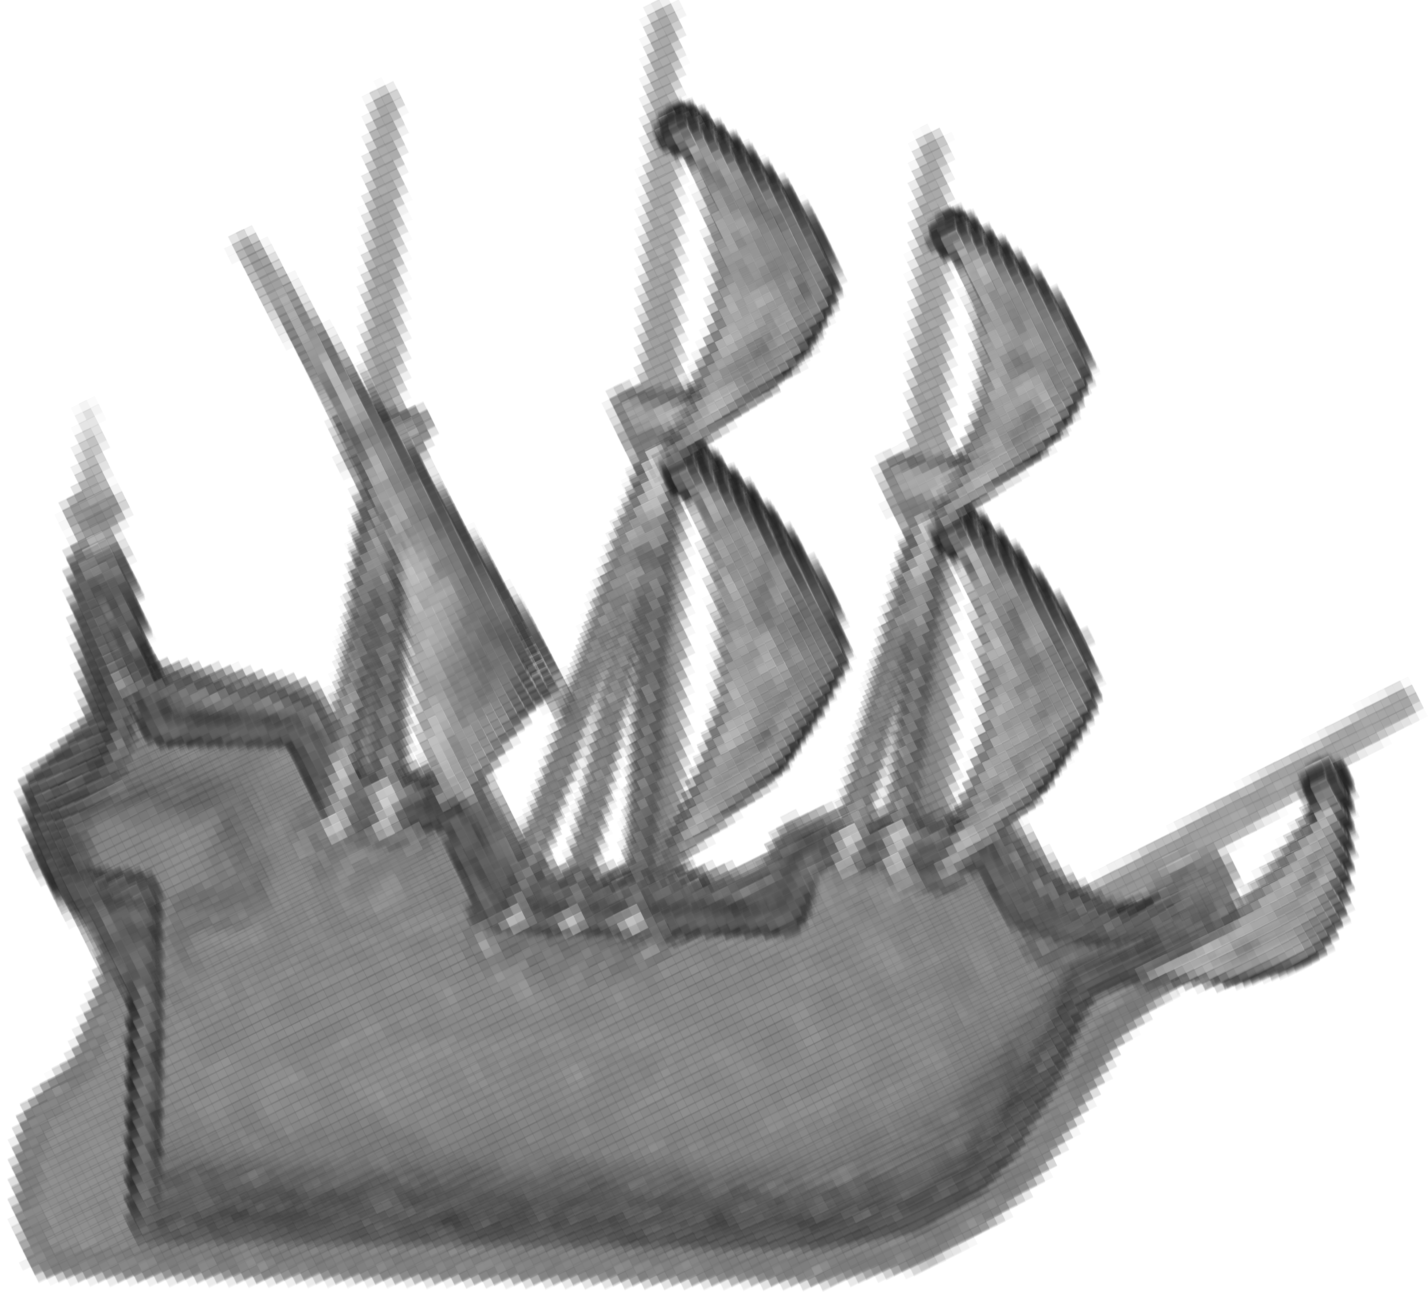
\includegraphics[width=1\linewidth]{./fig/eval/noise_none.png}
		\subcaption{$\sigma_{n} = 0$}
		\label{fig/eval/noise_none}
	\end{subfigure}
	\begin{subfigure}[t]{0.24\linewidth}\centering
		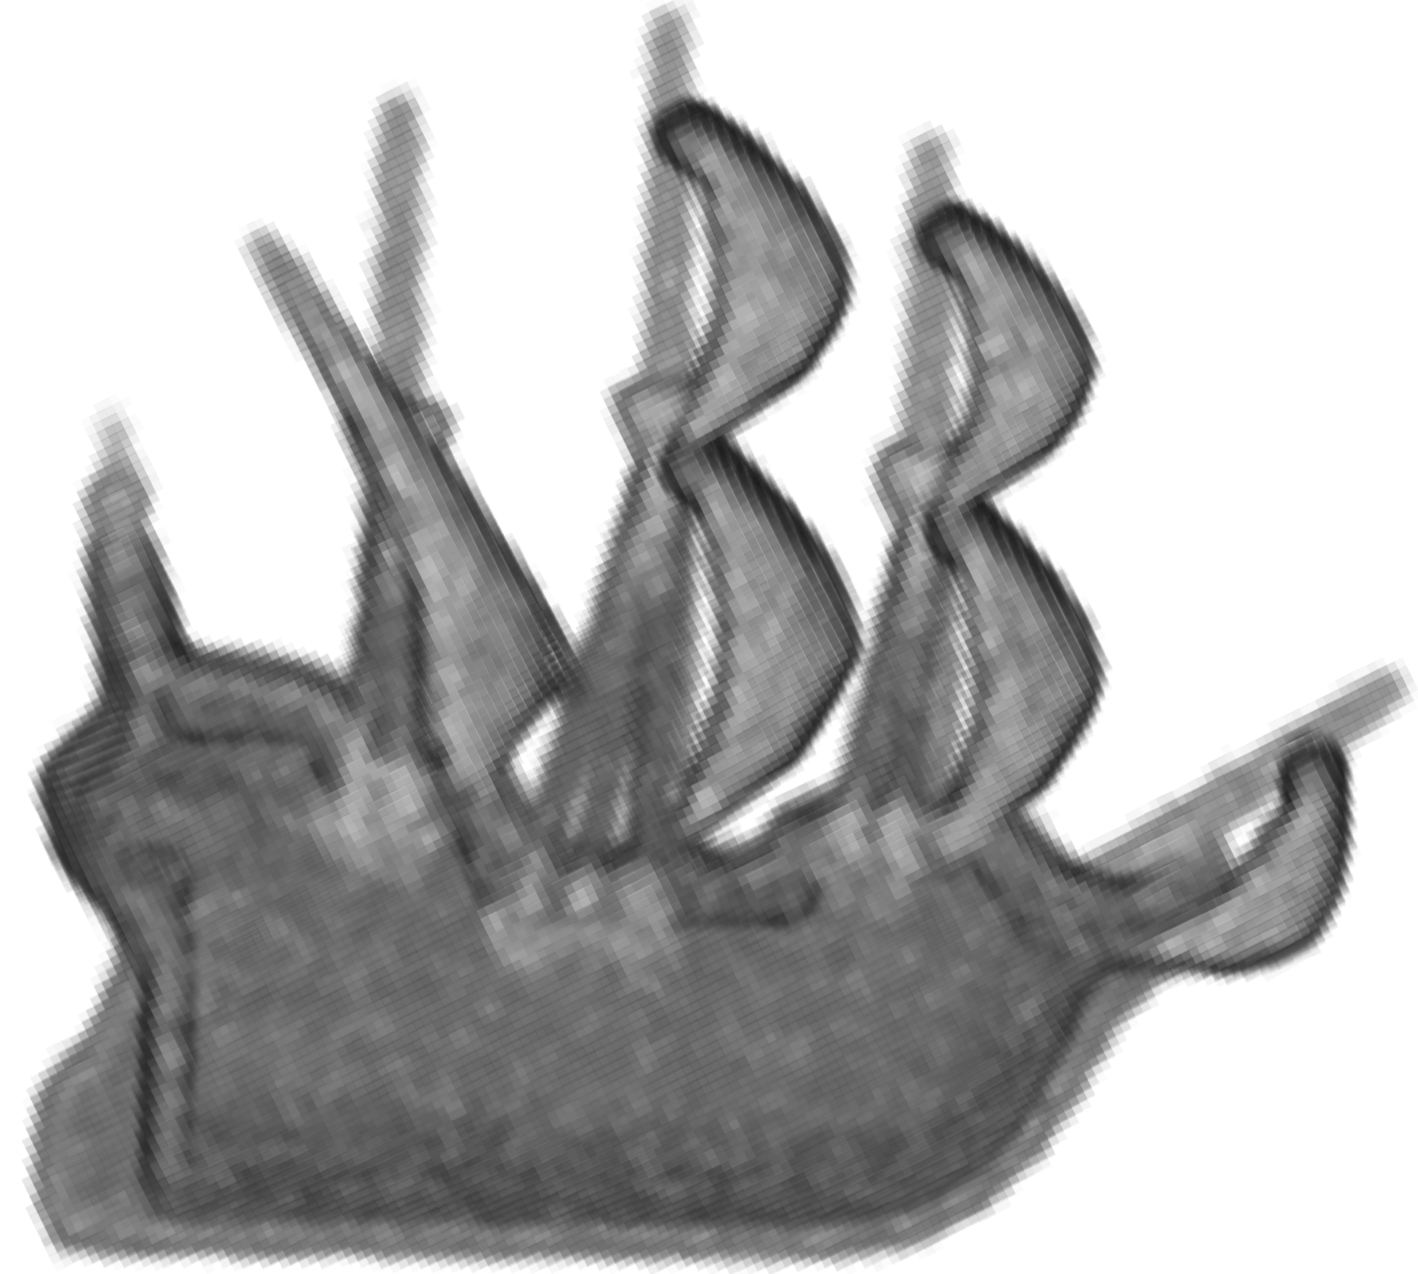
\includegraphics[width=1\linewidth]{./fig/eval/noise_low.png}
		\subcaption{$\sigma_{n} = 0.0025L$}
		\label{fig/eval/noise_low}
	\end{subfigure}
	\begin{subfigure}[t]{0.24\linewidth}\centering
		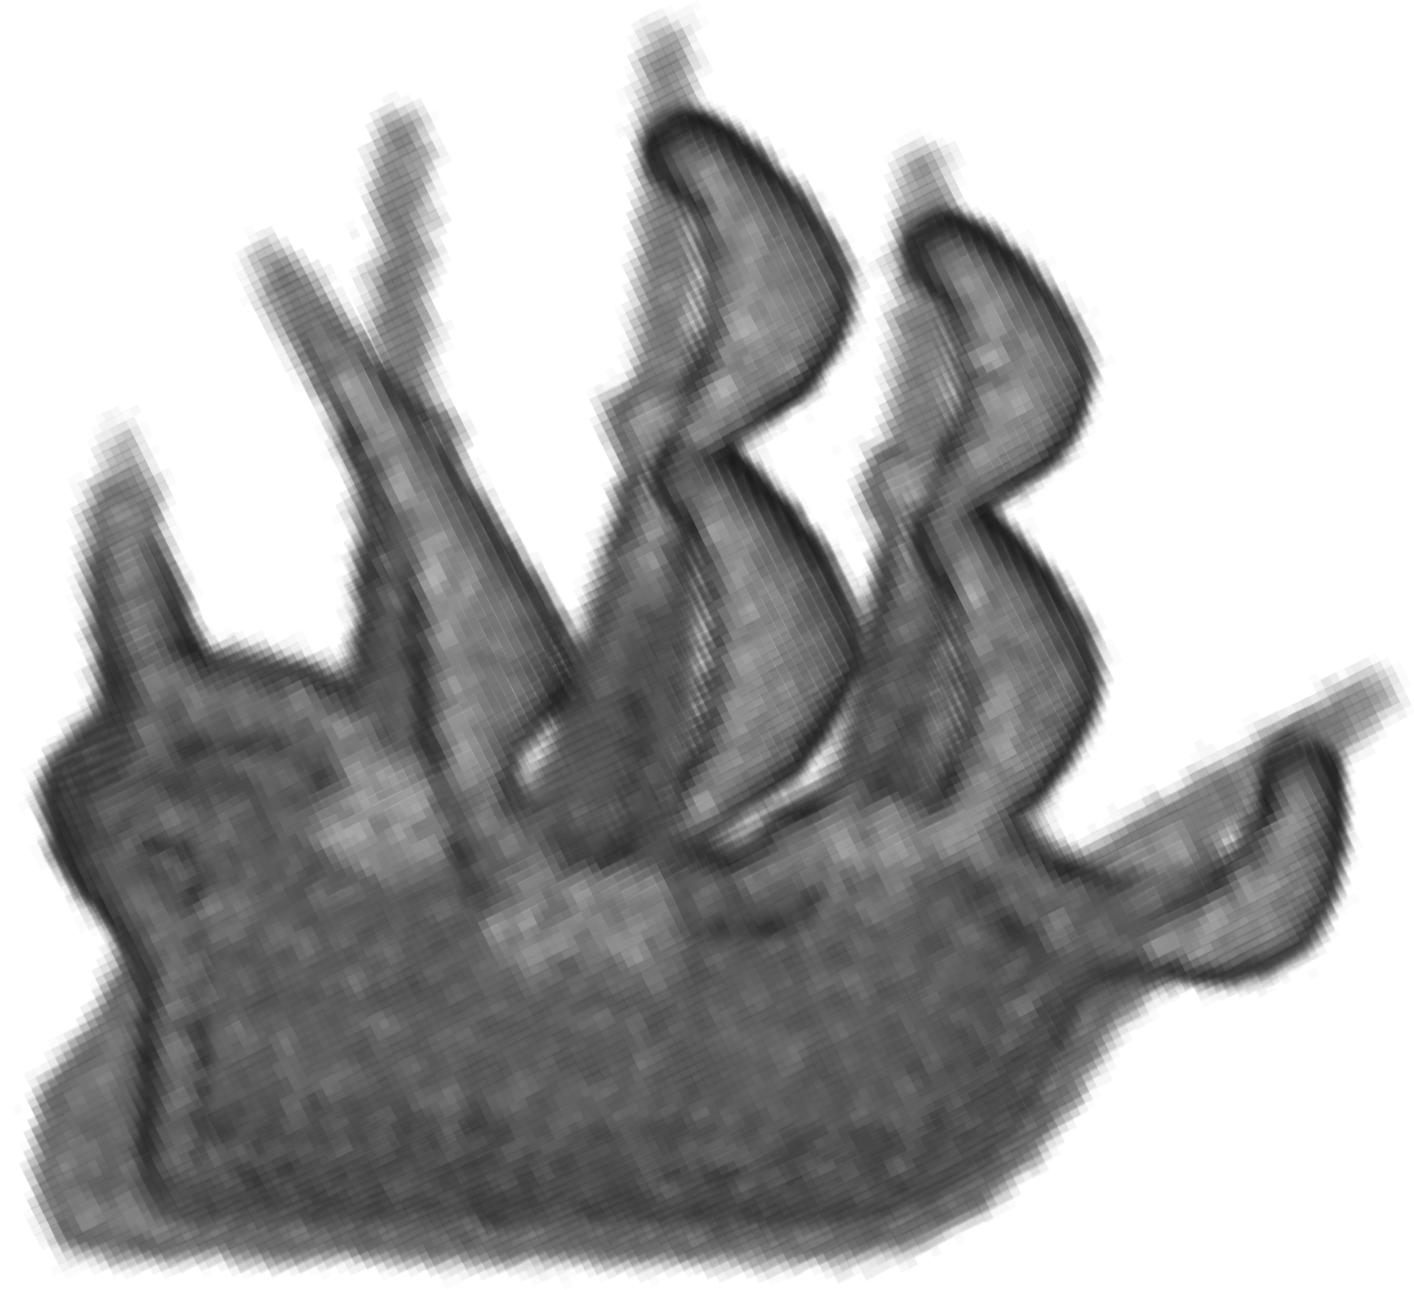
\includegraphics[width=1\linewidth]{./fig/eval/noise_mid.png}
		\subcaption{$\sigma_{n} = 0.01L$}
		\label{fig/eval/noise_mid}
	\end{subfigure}
	\begin{subfigure}[t]{0.24\linewidth}\centering
		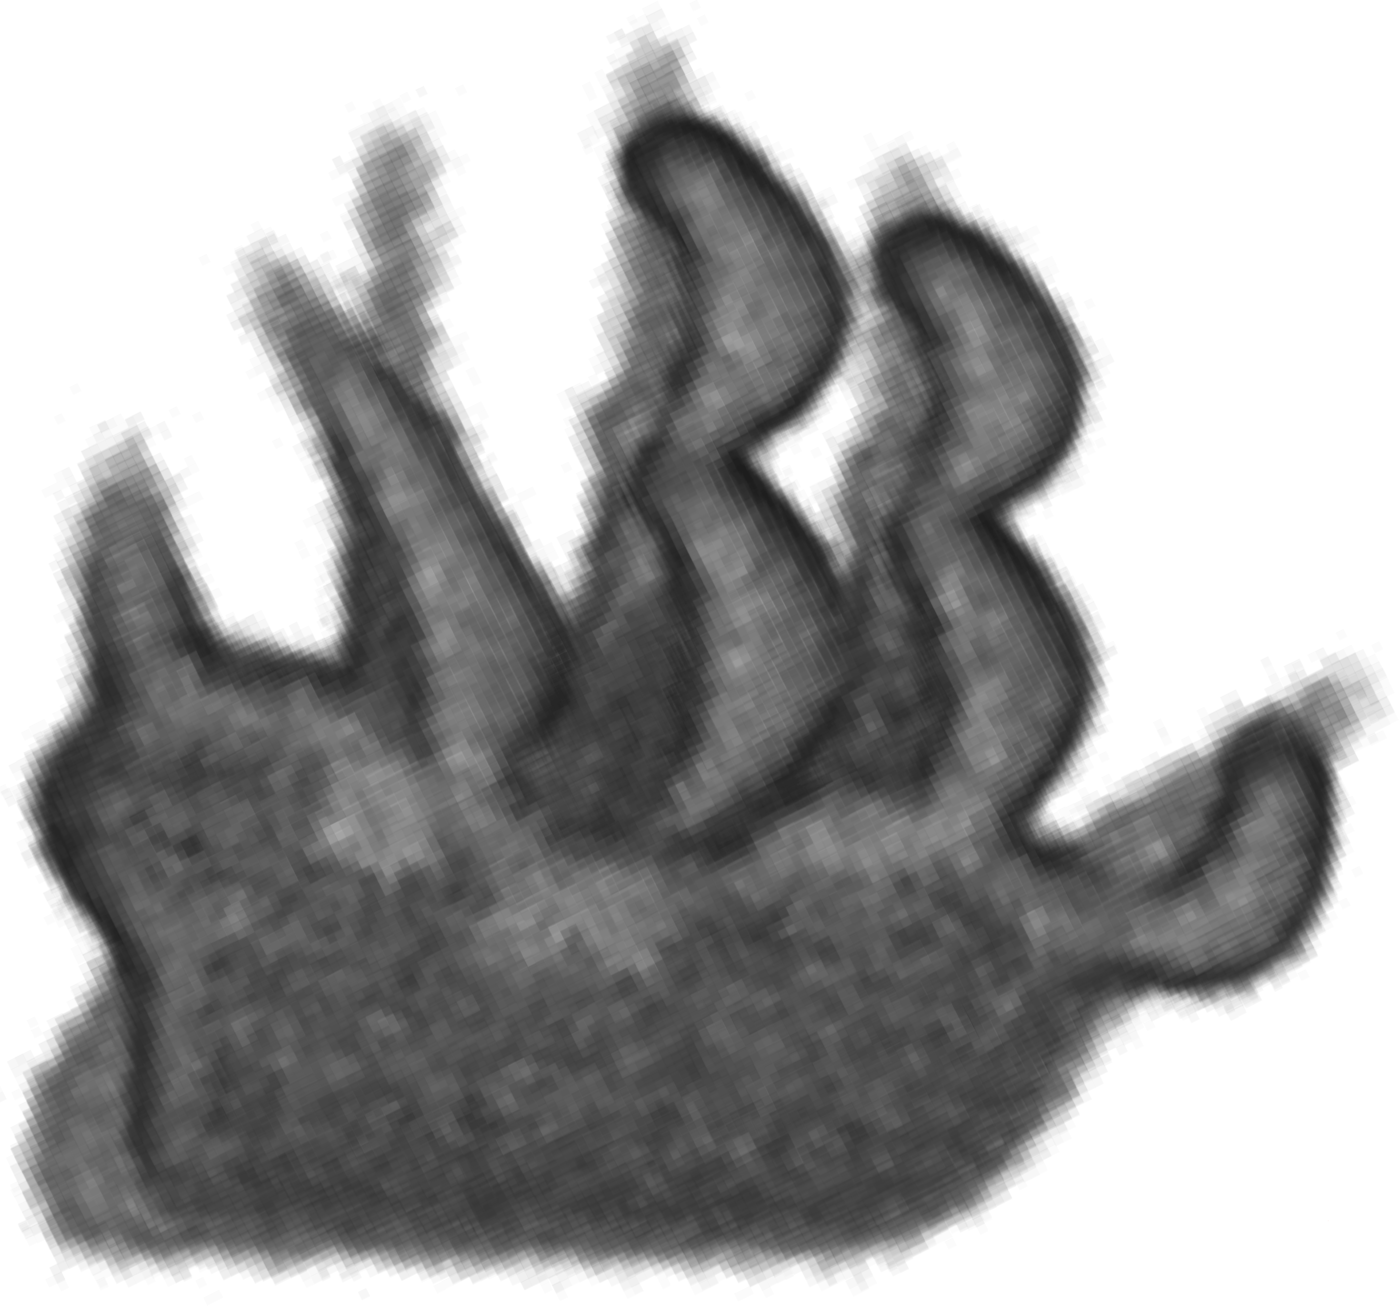
\includegraphics[width=1\linewidth]{./fig/eval/noise_high.png}
		\subcaption{$\sigma_{n} = 0.02L$}
		\label{fig/eval/noise_high}
	\end{subfigure}
	\caption{The ``galleon'' shape from the \meshset dataset, with different levels of sampling noise. The shape details disappear gradually as the noise level increases.}
	\label{fig/eval/noisesample}
\end{figure}

% done
Sampling noise and density are crucial factors in 3D interest point detection. As most of the 3D data acquisition techniques rely on shape reconstruction from point clouds or tomograms, existing shape acquisition techniques, such as multi-view stereo and 3D ultrasound, often produce data with high signal-to-noise ratio. 

% done 
In the sampling noise test, different levels of Gaussian white noise, with standard deviations $\sigma_{n}$ from $0L$ to $0.03L$, were applied to the \meshset dataset. Figure \ref{fig/eval/noisesample} shows the effect of sampling noise to a sample shape, detailed shape features disappears gradually as sampling noise level increases. 
The quantitatiev experimental result is displayed in figure \ref{fig/eval/graph_noise}. MSER outperforms other interest points, demonstrating high robustness. While the $\areascore$ scores of other detectors declined rapidly, MSER still achieved a high $\areascore$ score. The DoH detector showed a relatively stronger tolerance than detectors like SURF, Harris and VFAST. In contrast, the SURF detector had almost no repeatable point when sampling noise was higher than $6.5\%L$.

\subsubsection{Sampling density}

% done
In this experiment, the $\areascore$ score of shapes with various sampling densities were measured. Point clouds were randomly sampled from the input meshes, with point cloud sizes ranging from $4$K points to $405$K points. The sampling density directly affected voxelisation process of the point clouds, loss of details and holes were observed in point clouds of low sampling densities. 

% done 
Figure \ref{fig/eval/graph_sample} presents the change of $\areascore$ scores versus point cloud size. The scores vary linearly in log scale, thus a diminishing return is observed with increasing sampling density. MSER achieved the best average performance but it also had the largest variance across different shapes. In addition, DoH and DoG produced satisfactory results, with high scores but smaller intra-dataset variance than that of MSER.

% done 
\begin{figure}[ht]
	\centering 
	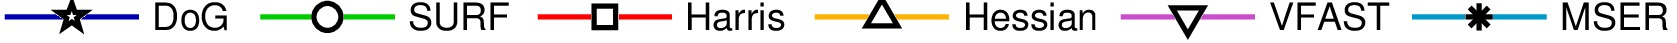
\includegraphics[width=0.70\linewidth]{./fig/eval/hlegend.jpg}
	\begin{subfigure}[t]{0.48\linewidth}
		\centering 
		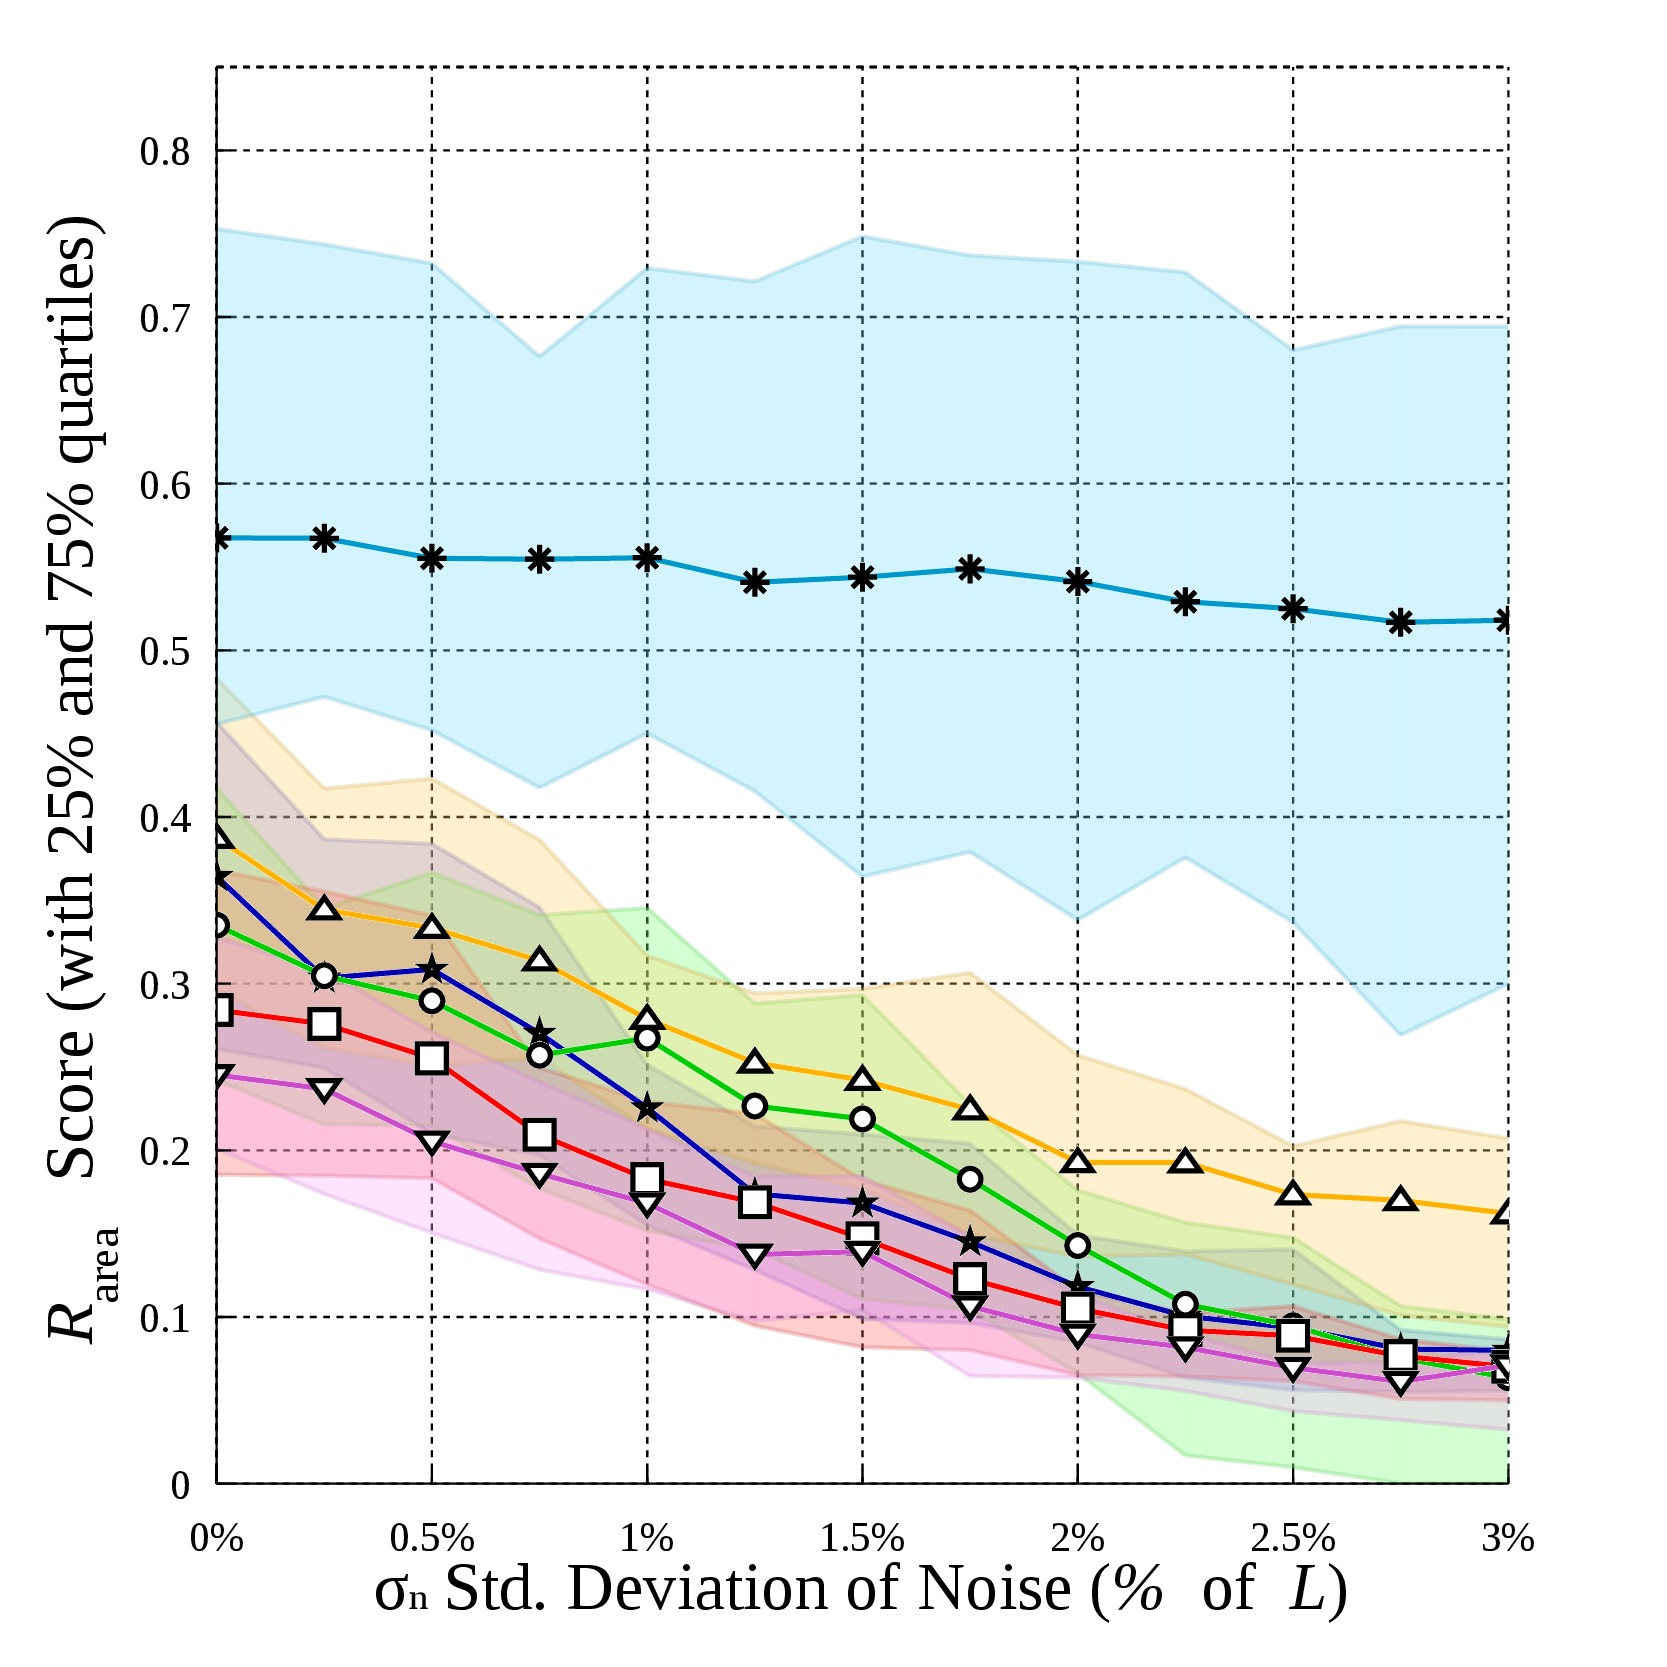
\includegraphics[width=1\linewidth]{./fig/eval/graph_noise.jpg}
		\subcaption{Sampling noise}
		\label{fig/eval/graph_noise}
	\end{subfigure}
	\begin{subfigure}[t]{0.48\linewidth}
		\centering 
		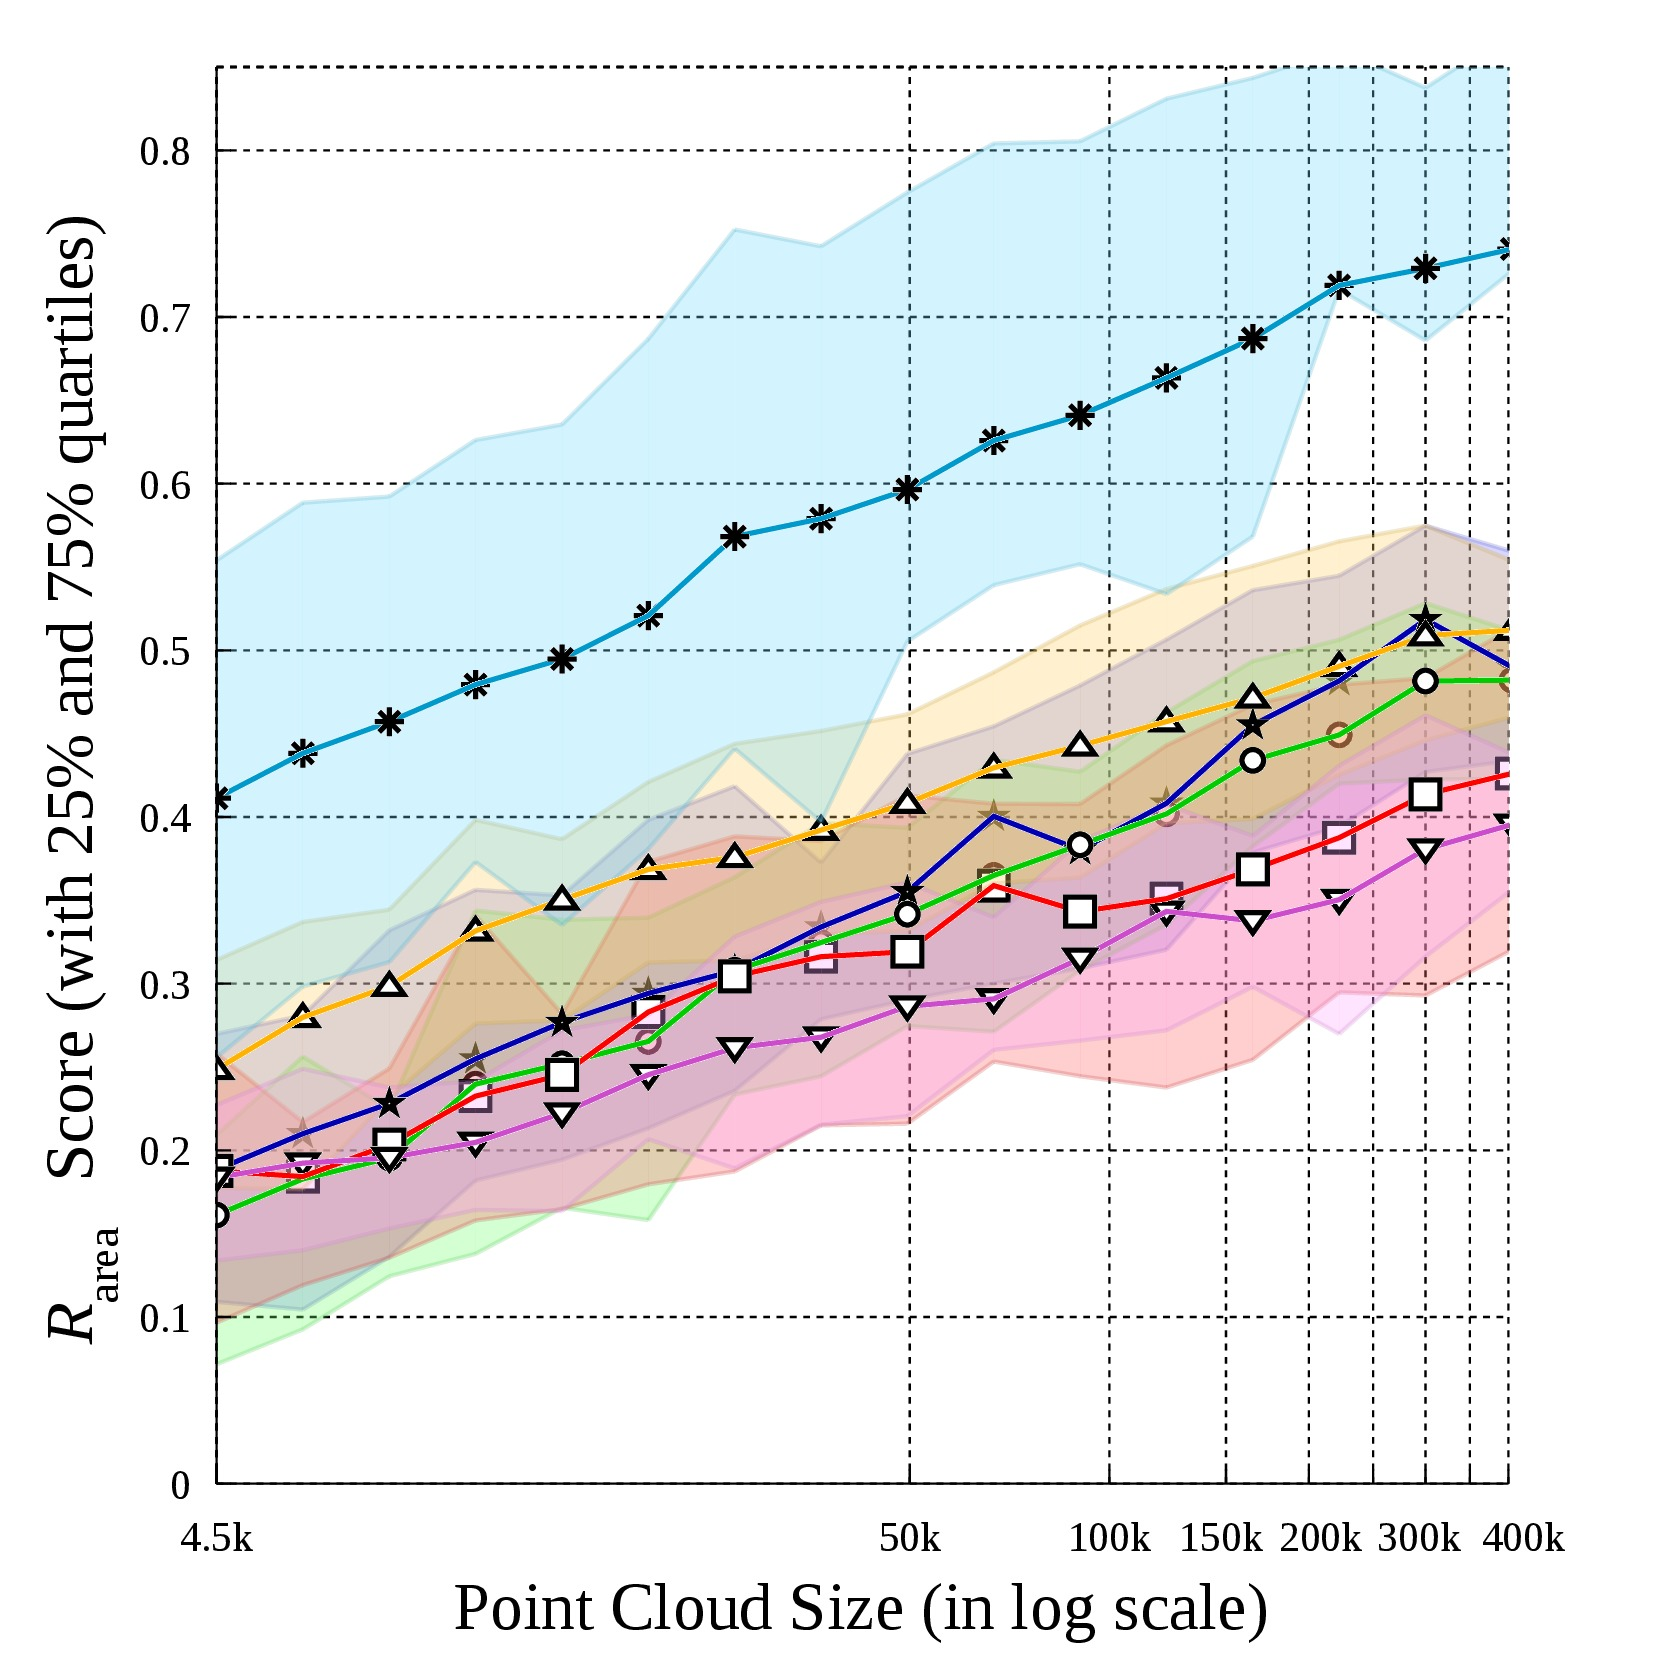
\includegraphics[width=1\linewidth]{./fig/eval/graph_sampling.jpg}
		\subcaption{Sampling density}
		\label{fig/eval/graph_sample}
	\end{subfigure}
	\caption{$\areascore$ scores of \meshset dataset under changing (a) sampling noise, (b) sampling density (point cloud size). Solid lines indicate the average $\areascore$ score.}
	\label{fig/eval/graph_graph0} 
\end{figure}

\subsubsection{Rotation}

% done 
This experiment evaluated the robustness of the candidate detectors to rotational aliasing effects. For each step of rotation angle, an average $\areascore$ score was computed by matching the testing shapes multiple times using different rotation axes, making the evaluation results unbiased. Eight rotation axes were generated randomly for each shape, and rotations of increasing magnitude, up to $90^\circ$, were applied to them and then the reference shapes. 

% done 
The effect of rotation is shown in figure \ref{fig/eval/graph_rotation}. Most detectors show excellent tolerance to rotation, inheriting this from their image-based counterparts. 
DoG and MSER performed slightly better than others, with stable average $\areascore$ score over a wide range of rotation angles. SURF performed worse than other volumetric interest point because the use of box filters has introduced extra quantisation errors when the shapes are rotated.

\subsubsection{Scale}

% done 
In this experiment, dimensions of voxelised input data were scaled from $50\%$ to $200\%$ of their original sizes. For fairness of evaluation, the transformed shapes were not directly interpolated from their voxelised reference shapes using interpolation. Rather, input point clouds were re-voxelised with varying volume dimensions $L$, whilst other parameters remained unchanged. 

% done 
Figure \ref{fig/eval/graph_scaling} illustrates the average $\areascore$ measured against different scale changes. 
From the experimental results, DoG and DoH detectors were comparatively more robust to scale. SURF only worked well at $100\%$ and its performance dropped rapidly outside the original scale, because of the approximated scale-space used. MSER achieved the best result at its original size, but its performance worsened steadily when the shape was resized.
Repeatability scores of all detectors dropped faster in downsampled volumes (scale $< 100\%$) than in upsampled volumes (scale $> 100\%$). 
This was because information content of smaller shape features was discarded when the input volume is downsized.   
In addition, the scale-space did not cover any feature with a size smaller than the first octave, therefore fine details were undetected.  
Meanwhile, the performance of most detectors decreased slowly as scale increased, when some features become too large to be detected. 
\begin{figure}[ht]
	\centering 
	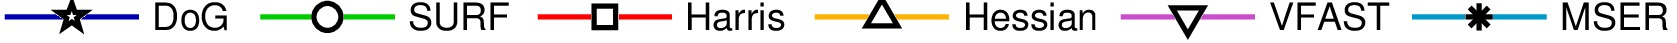
\includegraphics[width=0.70\linewidth]{./fig/eval/hlegend.jpg}
	\begin{subfigure}[t]{0.48\linewidth}
		\centering 
		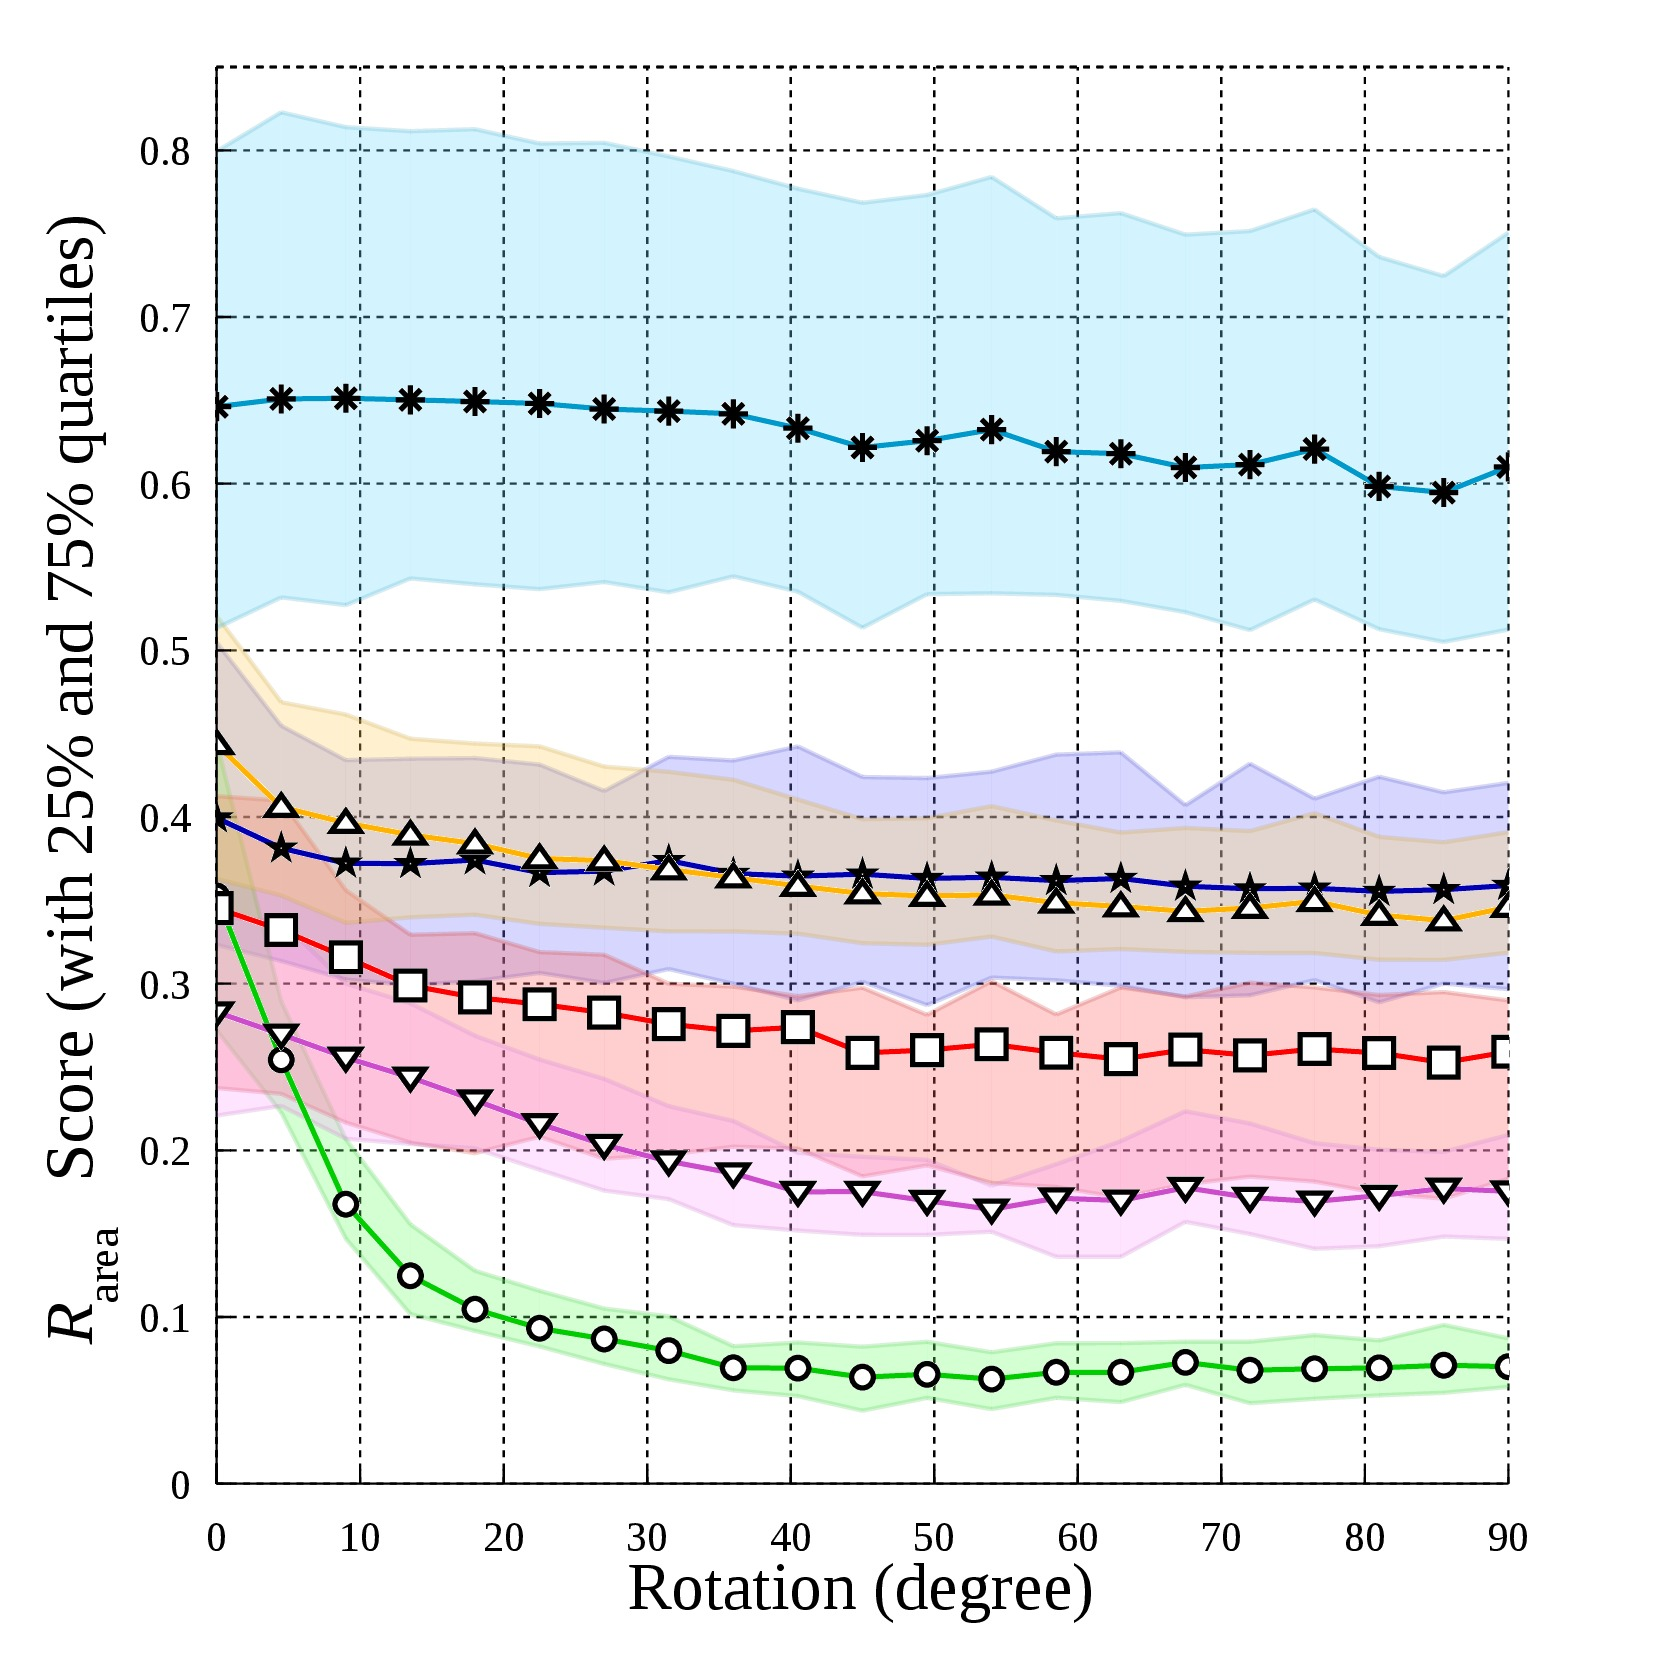
\includegraphics[width=1\linewidth]{./fig/eval/graph_rotation.jpg}
		\subcaption{Rotation}
		\label{fig/eval/graph_rotation}
	\end{subfigure}
	\begin{subfigure}[t]{0.48\linewidth}
		\centering 
		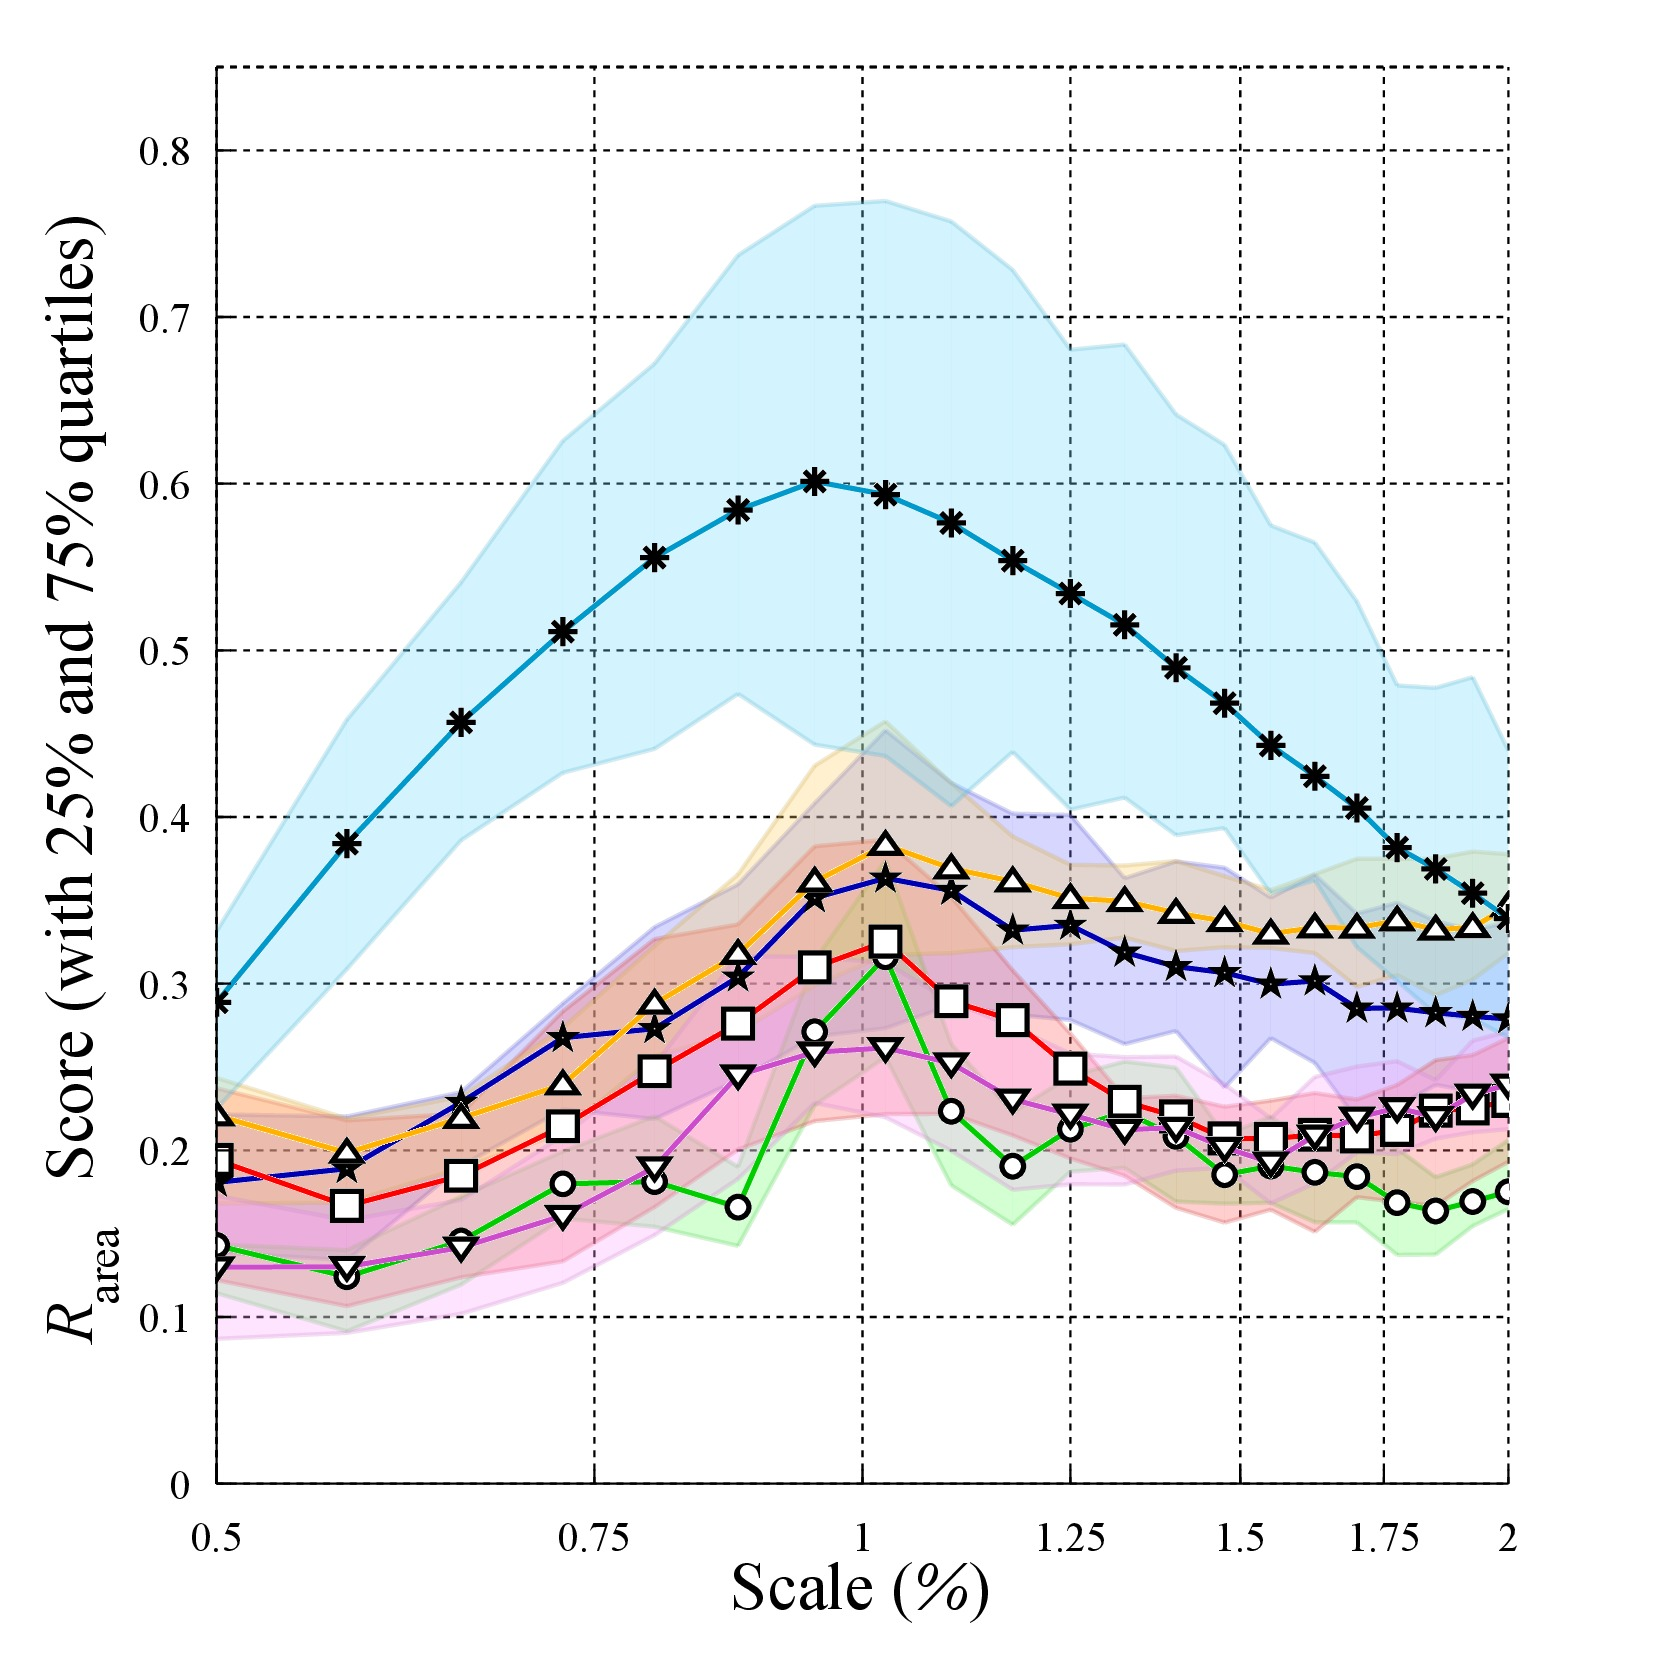
\includegraphics[width=1\linewidth]{./fig/eval/graph_scaling.jpg}
		\subcaption{Scale}
		\label{fig/eval/graph_scaling}
	\end{subfigure}
	\caption{$\areascore$ scores of \meshset dataset under varying (a) rotation, (b) scale. Solid lines indicate the average $\areascore$ score.}
	\label{fig/eval/graph_graph1} 
\end{figure}

\subsubsection{Number of corresponding interest points}

Table \ref{tab/eval/numcorr} presents quantitative statistics for the number of interest points and correspondences at three noise levels ($0.0025L$, $0.01L$ and $0.02L$), \cf figure \ref{fig/eval/noisesample}.
The MSER detector obtained the highest percentage of correspondences, yet it produced a smaller set of interest points. By contrast, DoH, SURF and Harris produced larger sets of interest points with good correspondence ratios. The displacement threshold used in this experiment ($\disp = 0.015L$) was about half the typical value, hence only the highly accurate correspondences were counted towards the values in the table. 

\begin{table}[ht]
	\centering
	\begin{tabular}{cc|ccc}
\hline
& & \multicolumn{3}{c}{\textbf{Sampling Noise Level}}  \\
& &  {\textbf{Low}}  & {\textbf{Medium}}  & {\textbf{High}}  \\
& & ($0.0025L$) & ($0.01L$) & ($0.02L$) \\
\hline
\hline
\multirow{3}{*}{DoG}  & Avg. \# Pts. &   122.0 & 118.2 & 73.1 \\
& Avg. \# Corr. &  48.8 & 35.1 &  9.3 \\
& (Corr. \%) & (\textit{39.8\%}) & (\textit{29.7\%}) & (\textit{12.7\%}) \\
\hline
\multirow{3}{*}{SURF} & Avg. \# Pts. & 154.7 & 70.4  & 28.7 \\
& Avg. \# Corr. &  54.7 & 18.4  & 3.84 \\
& (Corr. \%) &  (\textit{35.3\%}) & (\textit{26.2\%})  & (\textit{13.4\%}) \\
\hline
\multirow{3}{*}{Harris} & Avg. \# Pts. & 303.3 & 142.2 &  123.8 \\
& Avg. \# Corr. & 78.6  & 33.2  &    13.4  \\
& (Corr. \%) & (\textit{25.9\%}) & (\textit{23.3\%}) & (\textit{10.83\%}) \\
\hline
\multirow{3}{*}{DoH}& Avg. \# Pts. &  {\textbf{\color{blue}330.8}} & {\textbf{\color{blue}272.0}} &   {\textbf{\color{blue}201.2}} \\
& Avg. \# Corr. & {\textbf{\color{blue}117.1}} & {\textbf{\color{blue}72.2}}  &   {\textbf{\color{blue}30.2}} \\
& (Corr. \%) & (\textit{35.4\%}) & (\textit{26.6\%}) & (\textit{18.2\%}) \\
\hline
\multirow{3}{*}{VFAST}& Avg. \# Pts. &  115.9 &  85.5  &  74.6\\ 
& Avg. \# Corr. & 33.5  & 15.5  &    7.4 \\
& (Corr. \%) & (\textit{28.8\%}) & (\textit{18.10\%})  & (\textit{9.85\%}) \\
\hline
\multirow{3}{*}{MSER}& Avg. \# Pts.  &  99.0  & 74.4  &   52.5 \\
& Avg. \# Corr. & 59.9 & 44.7  &   28.8 \\
& (Corr. \%) & ({\textit{\textbf{\color{blue}60.5}}\%})  & ({\textit{\textbf{\color{blue}60.2}}\%})  & ({\textit{\textbf{\color{blue}54.9}}\%})\\
\hline
\end{tabular}
\caption{For each entry, top to bottom: The average number of interest points detected, the average number of correspondences, percentage of points with correspondences.}
\label{tab/eval/numcorr}
\end{table}


\subsubsection{Saliency}

% done 
Figure \ref{fig/eval/graph_keypointnum} shows the repeatability ratio, $R_\textrm{ratio}$, with varying percentages of interest points. For each detector, interest points were detected and sorted by their corresponding saliency responses in descending order, afterwards the first $p\%$ of interest points were used to calculate $R_\mathrm{ratio}$. However, since no saliency measure has been defined in the MSER detector, the number of detected interest points could not be controlled directly; MSER was therefore not included in figure \ref{fig/eval/graph_keypointnum}. Similar to the previous test on correspondences, $R_\textrm{ratio}$ was computed using a smaller displacement threshold ($\disp = 0.015L$) in this experiment.   

% done 
The performances of DoG and Harris detectors tended to be stable, though Harris performed notably worse than DoG, with increasing numbers of interest points, \ie decreasing saliency threshold. The results indicated that a saliency threshold was not necessary for these detectors. In other words, the saliencies of DoG and Harris did not reflect their potential repeatabilities. The performance of DoH, which was initially the best, decreased very slowly and converged with DoG and SURF, indicating that the lower saliency points were less reliable. A saliency threshold for DoH would benefit applications requiring more accurate point localisation. By contrast, the reapeatability scores of SURF and VFAST increased steadily before leveling off, suggesting that some of the high saliency points were unreliable. this would pose more of a problem in terms of interest point selection. 

\begin{figure}[ht]
	\centering
	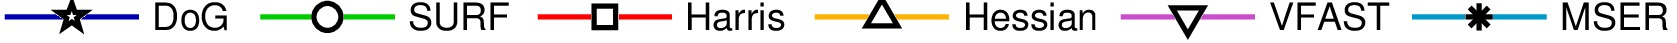
\includegraphics[width=0.70\linewidth]{./fig/eval/hlegend.jpg} \\ 
	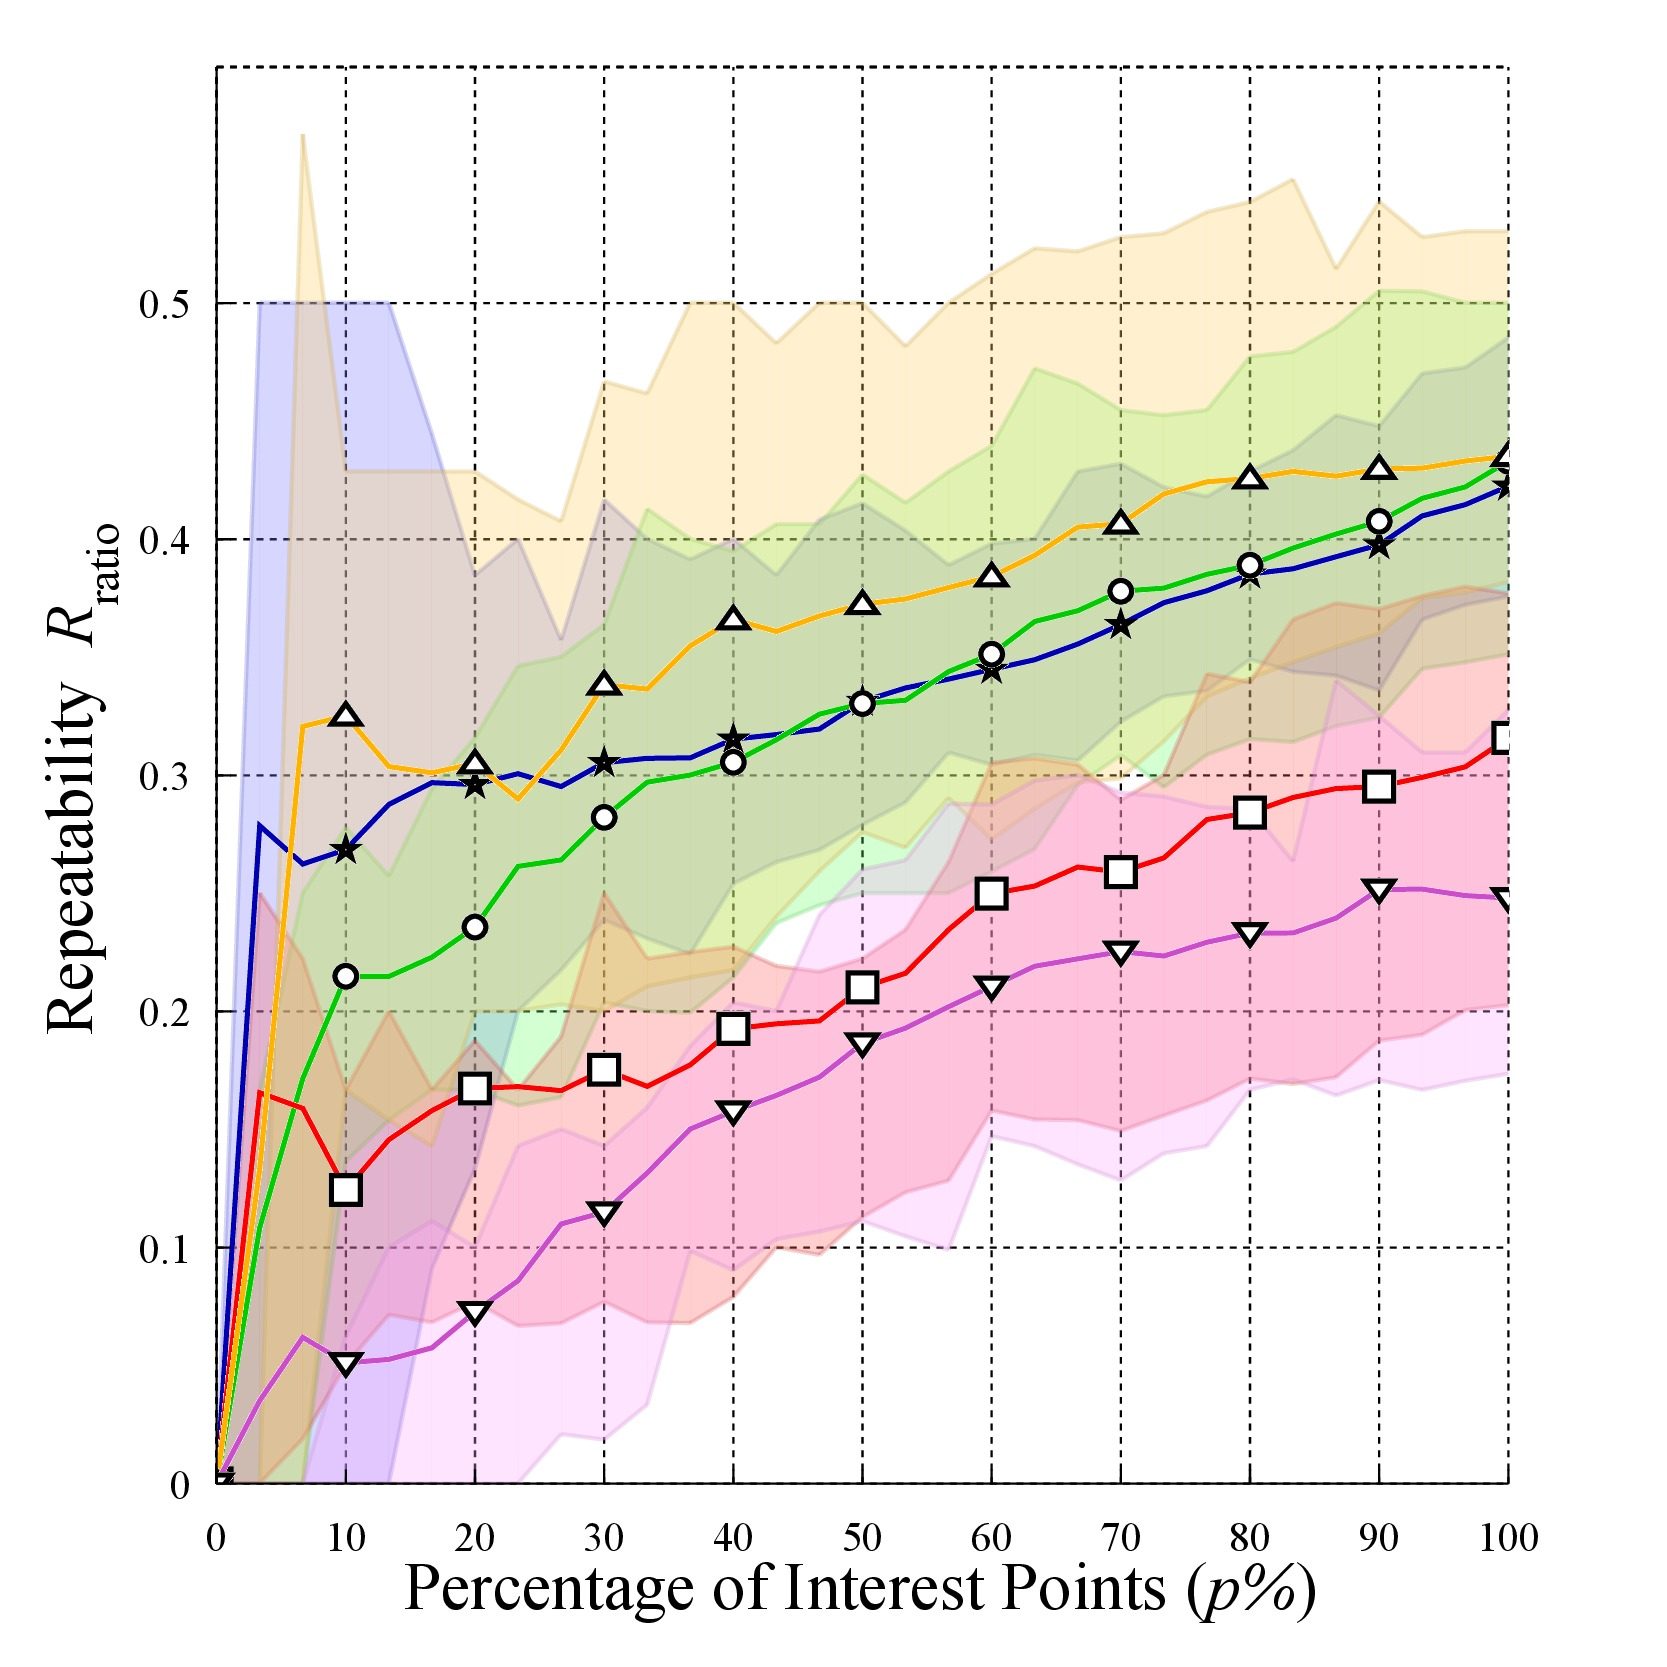
\includegraphics[width=0.48\linewidth]{./fig/eval/graph_keypointnum.jpg}
	\caption{$\areascore$ scores of the \meshset dataset with varying percentage of interest points}
	\label{fig/eval/graph_keypointnum}	
\end{figure}

\subsection{Experiments on MRI and stereo data}

% done 
Interest points detectors were also evaluated on the \mriset and \stereoset datasets. As a reference for cross validation, average scores obtained from the \meshset dataset are plotted against displacement threshold $\disp$ in figure \ref{fig/eval/graph_syn}. 

% done 
\subsubsection{MRI dataset} This dataset contains two MRI scans of a human brain, each MRI has the longest dimension $L$ of $218$ voxels.
Figure \ref{fig/eval/mri} shows the MSER interest points detected in the data. It is worth noting that some points detected on the MRIs were matched easily, such as those on the nose-tips, eye sockets and foreheads, but that there were fewer detections within the brain area, which consisted of voxels with smaller intensity variations.

% done 
The $\areascore$ scores were measured from the \mriset dataset with varying $\disp$ in figure \ref{fig/eval/graph_mri}. The evaluation results were comparable to that of synthetic mesh data. MSER, DoG and DoH attained slightly better performances in synthetic meshes, while the Harris detector was good at detecting complicated internal structures in the MRI scans. 

\begin{figure}[ht]
	\centering 
	\begin{subfigure}[t]{0.35\linewidth} \centering 
		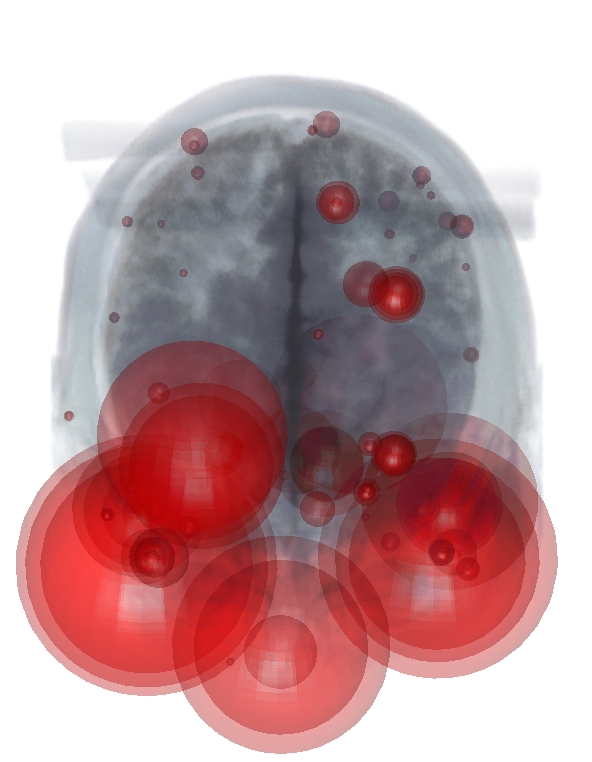
\includegraphics[width=0.8\linewidth]{./fig/eval/mri.png}
		\subcaption{MRI scane 1}
		\label{fig/eval/mri1}
	\end{subfigure}
	\begin{subfigure}[t]{0.35\linewidth} \centering 
		\includegraphics[width=0.8\linewidth]{./fig/eval/mri2.png}
		\subcaption{MRI scane 2}
		\label{fig/eval/mri2}
	\end{subfigure}
	\caption{Two MRI scans of a human brain, with detected MSER features}
	\label{fig/eval/mri}
\end{figure}

\subsubsection{Stereo dataset} 

\begin{figure}
	\centering
	\begin{subfigure}[t]{0.23\linewidth} \centering
		\includegraphics[width=1\linewidth]{./fig/eval/toshiba_bearing1.png}
		\subcaption{Bearing}
	\end{subfigure}
	\begin{subfigure}[t]{0.23\linewidth} \centering
		\includegraphics[width=0.8\linewidth]{./fig/eval/toshiba_bracket1.png}
		\subcaption{Bracket}
	\end{subfigure}
	\begin{subfigure}[t]{0.23\linewidth} \centering
		\includegraphics[width=1\linewidth]{./fig/eval/toshiba_flange1.png}
		\subcaption{Flange}
	\end{subfigure}
	\begin{subfigure}[t]{0.23\linewidth} \centering
		\includegraphics[width=1\linewidth]{./fig/eval/toshiba_knob1.png}
		\subcaption{Knob}
	\end{subfigure}
	\begin{subfigure}[t]{0.23\linewidth} \centering
		\includegraphics[width=1\linewidth]{./fig/eval/toshiba_mini1.png}
		\subcaption{Car}
	\end{subfigure}
	\begin{subfigure}[t]{0.23\linewidth} \centering
		\includegraphics[width=1\linewidth]{./fig/eval/toshiba_pipe1.png}
		\subcaption{Pipe}
	\end{subfigure}
	\begin{subfigure}[t]{0.23\linewidth} \centering
		\includegraphics[width=1\linewidth]{./fig/eval/toshiba_piston1.png}
		\subcaption{Piston 1}
	\end{subfigure}
	\begin{subfigure}[t]{0.23\linewidth} \centering
		\includegraphics[width=1\linewidth]{./fig/eval/toshiba_piston2.png}
		\subcaption{Piston 2}
	\end{subfigure}
	\caption{Rendered CAD models of the \stereoset dataset} 
	\label{fig/eval/mvscad}
\end{figure}

% done 
Sixteen point clouds were captured using a multi-view stereo technique \cite{Vogiatzis2011} from realistic, 3D-printed CAD models. The point clouds were converted into volumes with maximum length $L$ of $132$ voxels. Figure \ref{fig/eval/mvscad} shows the rendered CAD models from the \stereoset dataset; figure \ref{fig/eval/mvs} visualises different types of interest points detected on their corresponding voxelised shapes.

% done 
The $\areascore$ scores obtained from the \stereoset dataset, shown in figure \ref{fig/eval/graph_mvs}, were lower compared with \meshset and \mriset datasets, especially at a small matching threshold $\disp$. Nonetheless, in terms of overall rankings and relative scores of the detectors, synthetic and real data showed similar behaviours. The decrease in performance for stereo data were due to its: (a) low sampling frequency and high noise, (b) uneven object surfaces, which are infeasible for blob detection algorithms, such as MSER, SURF and DoH, and (c) small errors in the estimated ground truth poses from ICP alignment.
The differences in $\areascore$ scores were due to occlusions, viewpoint changes and uneven sampling density of the \stereoset dataset. 

% done 
Some testing instances, \eg ``car'' in figure \ref{fig/eval/mvs}, had a much sparser point cloud due to a lack of texture on the object's surface, but the distribution of detected features was no less dense across any of the detectors, suggesting that the experimental results of the synthetic datasets are representative of sparse point clouds as well as dense ones.

\begin{figure}[ht]
	\centering
	\includegraphics[width=0.80\linewidth]{./fig/eval/hlegend.jpg}\\
	\begin{subfigure}[t]{0.49\linewidth}
		\centering 
		\includegraphics[width=0.95\linewidth]{./fig/eval/graph_oneshape.jpg}
		\subcaption{$\areascore$ score: \meshset}		
		\label{fig/eval/graph_syn}
	\end{subfigure}
	\begin{subfigure}[t]{0.49\linewidth}
		\centering 
		\includegraphics[width=0.95\linewidth]{./fig/eval/graph_mri.jpg}
		\subcaption{$\areascore$ score: \mriset}		
		\label{fig/eval/graph_mri}
	\end{subfigure}
	\begin{subfigure}[t]{0.49\linewidth}
		\centering 
		\includegraphics[width=0.95\linewidth]{./fig/eval/graph_stereo.jpg}
		\subcaption{$\areascore$ score: \stereoset}		
		\label{fig/eval/graph_mvs}
	\end{subfigure}
\caption{$\areascore$ scores versus displacement threshold $d$. Left to right: (a) \meshset dataset, (b) \mriset dataset and (c) \stereoset dataset.}
\label{fig/eval/graph2}
\end{figure}

\subsection{Computation time}

% done
Computation efficiency is also a crucial factor for choosing a suitable interest point detector for a particular computer vision application. Since the storage size of volumetric data is usually much larger than 2D images, the time and memory complexities of the interest point detectors increase accordingly. Operations which are considered efficient for 2D images can become much slower for 3D volumetric data. For non-volumetric input data such as point clouds, extra computation time is required to voxelise the shape. 

% done 
On the other hand, some interest point detectors can be accelerated by parallel processing techniques, using specialised hardware, such as GPUs and FPGAs \cite{Sinha2006, Cornelis2008, Teixeira2008, Bhatia2007, Dohi2011, Kristensen2007}. Table \ref{tab/eval/speedtable} summarises the algorithmic complexities of the candidate detectors and the time required for them to compute interest points on the \meshset dataset. From left to right, (1) it lists the algorithmic complexities, (2) the average processing time for the \meshset dataset, (3) potential parallel implementations and (4) existing machine learning-based acceleration. 
In order to compare the speed performance in a common evaluation framework, all candidate detectors were implemented in MATLAB, without any hardware acceleration. The experiments were performed on the same hardware platform (Intel Core i7, $12$GB RAM). 

\begin{table}
\centering
\begin{tabular}{c|cccc}
\hline
\textbf{Interest} & \textbf{Complexity} & \textbf{Speed} & \textbf{Parallelizable} & \textbf{Machine} \\
\textbf{Point} & & \textbf{($\mu$s / voxel)} & & \textbf{learning} 	\\ 	
\hline
DoG 		& $O(SN)$ 			& $1.325 $ 			& \checkmark \cite{Sinha2006} & \\
SURF 		& $O(SN)$ 			& $1.035 $ 			& \checkmark \cite{Cornelis2008} & \\
Harris 		& $O(SN)$ 			& $1.112 $ 			& \checkmark \cite{Teixeira2008} & \\
DoH			& $O(SN)$ 			& $1.325 $ 			& \checkmark \cite{Bhatia2007} \\
VFAST 		& $O(SN)$ 			& $1.670 $ 			& \checkmark \cite{Dohi2011} & \checkmark \cite{Rosten2010}\\
MSER 		& $O(N\log(\log(N)))$ 	& $2.070 $ 			& \checkmark \cite{Kristensen2007} &\\
\hline
\end{tabular}
\caption{Run-time performances of the candidate detectors, where $N$ denotes the number of voxels and $S$ is the number of octaves in the scale-space.}
\label{tab/eval/speedtable}
\end{table}

% done 
Theoretically, all detectors have a similar time complexity, except for MSER, which does not implement a Gaussian scale-space. The SURF detector is the fastest among the candidate detectors, as it uses Haar wavelets to accelerate the computation of Gaussian derivatives. Harris also shows high efficiency due to its relatively simple algorithm. MSER is the slowest detector, as the search algorithm for stable regions is less efficient in 3D volumes than in 2D images. Surprisingly, the VFAST detector is the second slowest detector in the experiment. Since FAST is a pixel/voxel-wise rule based algorithm, the accelerated segment test in equation \ref{eqn/eval/fastast} cannot utilise the high performance linear algebra routines used by other detectors such as DoG and SURF. Nonetheless, FAST detector can be accelerated by learning a decision tree classifier from training data \cite{Rosten2010}, which was not implemented in this experiment.

% done
\subsection{Qualitative analysis: blobs versus corners}
The candidate 3D interest point detectors can be roughly classified into three different categories: region-based blob detection (MSER), derivative-based blob detection (DoG, DoH and SURF) and corner detection (Harris, VFAST). The quantitative evaluation results has implied that region-based blob detectors work better than derivative-based blob detectors, and blob detectors are better than corner detectors, but 3D interest points cannot be evaluated by repeatability only. The candidate detectors also have different behaviours in terms of locations and scales of the interest points. Therefore, besides repeatability, it is also important to analyze the characteristics of detectors qualitatively. Figure \ref{fig/eval/mesh} visualises interest points detected by the six candidate detectors on the ``cat'' object from the \meshset dataset.

% done 
\subsubsection{Region-based blob detection} MSER detects contiguous regions of any shape, \ie not limited to spherical blobs, allowing it to select more robust regions from a greater selection, and hence perform better. MSER performs well in 3D shape data because the shapes of salient regions are inherently less susceptible to viewpoint changes. It can be seen in figures \ref{fig/eval/mesh/mser} and \ref{fig/eval/mvs/mser} that MSER found features at fewer locations, but over multiple scales. The locations tended to center on regions of high surface curvature.

% done 
\subsubsection{Derivative-based blob detection} Theoretically, DoG, DoH and SURF find, in order of preference, spherical blobs, corners and planes. In the experiments, DoG and DoH produced qualitatively similar output, as shown in figures \ref{fig/eval/mesh/dog}, \ref{fig/eval/mvs/dog}, \ref{fig/eval/mesh/hessian} and \ref{fig/eval/mvs/hessian}, finding features such as limb extremities in the \meshset dataset, or sharp corners in the \stereoset dataset, as well as inside shape such as the hull of ``galleon'' and the hole in ``knob''. By contrast, SURF, despite being an approximation of the DoH detector, produced features off the surface (both inside and outside), often over regions of low surface curvature, as shown in figure \ref{fig/eval/testshapes/surf}. Instead of highly repeatable features, derivative-based approaches produce more diverse features than region-based detectors. Finally, their repeatability scores degrade more rapidly than MSER for noisy input data in figure \ref{fig/eval/graph_noise}, mainly due to higher rates of false positive detections. 


\subsubsection{Corner detection} Harris and VFAST both aim to find areas of high curvature. However, their outputs (figures \ref{fig/eval/testshapes/harris} and \ref{fig/eval/testshapes/fast}) varied qualitatively, with the former tending to find fewer features and more sharp corners than the latter, which finds an even distribution of features over both scale and location. In general, corner detection approaches are relatively less robust to noise and transformations than blob detection techniques. Whilst blobs remain stable in noisy or transformed volumetric data, small scale features like corners are more easily affected by quantisation errors or sampling noise. 
The performance of blob detectors dropped faster than that of edge detectors at low (figure \ref{fig/eval/graph_sample}) and uneven (figures \ref{fig/eval/graph_syn} and \ref{fig/eval/graph_mvs}) sampling densities. Holes form on shape surfaces in these situations, creating false positives for both corner and blob detectors, however, the detection of true positives appears to be more robust for corner detectors in these cases. 
% Comparing the \meshset dataset and the \stereoset dataset, blob detectors have a greater drop in $\areascore$ score than corner detectors. It is because holes are formed on shape surfaces at a low or uneven sampling density, \eg \stereoset dataset in figure \ref{fig/eval/mvs}, they prevent the formation of stable blobs inside the cavities of a shape as in the \meshset dataset (figure \ref{fig/eval/mesh}). On the other hand, corner features are mainly detected at edges where the sampling density is generally higher than shape surfaces, thus they are less affected. Nevertheless, the unevenly sampled surface create false positives for all detectors, an overall drop in $\areascore$ score is therefore observed in \ref{fig/eval/mvs}. 
%Holes are formed on the shapes' surfaces at a low or uneven sampling density, \eg \stereoset dataset in figure \ref{fig/eval/graph_mvs}, creating false positives for both corner and blob detectors. These holes also prevents the formation of larger blobs. However, detection of corner features, which are usually smaller in size than blobs, are less affected. 
%On the other hand, since corner-based detectors use smaller local windows than blob-based methods, they are feasible for detecting interest points when blobs cannot be detected correctly in low sampling density (\emph{c.f.} figure \ref{fig/eval/graph_mvs}).

\begin{figure}[ht]
	\centering
	\begin{subfigure}[t]{1\linewidth}\centering
		\makebox[0.15\linewidth]{}
		\makebox[0.175\linewidth]{\textbf{Bicycle}}
		\makebox[0.155\linewidth]{\textbf{Kicking man}}
		\makebox[0.175\linewidth]{\textbf{Galleon}}
		\makebox[0.175\linewidth]{\textbf{Ant}}
	\end{subfigure}
	\begin{subfigure}[t]{1\linewidth} \centering 
		\phantomcaption 
		\label{fig/eval/mesh/input}	
		\makebox[0.15\linewidth]{\raisebox{0.07\linewidth}{(a) Input}} 
		\includegraphics[width=0.175\linewidth]{./fig/eval/cycle_input.jpg} 
		\includegraphics[width=0.155\linewidth]{./fig/eval/guy_input.jpg} 
		\includegraphics[width=0.175\linewidth]{./fig/eval/ship_input.jpg}
		\includegraphics[width=0.175\linewidth]{./fig/eval/ant_input.jpg} 
	\end{subfigure}
	\begin{subfigure}[t]{1\linewidth} \centering 
		\phantomcaption 
		\label{fig/eval/mesh/dog}	
		\makebox[0.15\linewidth]{\raisebox{0.07\linewidth}{(b) DoG}} 
		\includegraphics[width=0.175\linewidth]{./fig/eval/cycle_dog.jpg} 
		\includegraphics[width=0.155\linewidth]{./fig/eval/guy_dog.jpg} 
		\includegraphics[width=0.175\linewidth]{./fig/eval/ship_dog.jpg}
		\includegraphics[width=0.175\linewidth]{./fig/eval/ant_dog.jpg} 
	\end{subfigure}
	\begin{subfigure}[t]{1\linewidth} \centering 
		\phantomcaption 
		\label{fig/eval/mesh/surf}	
		\makebox[0.15\linewidth]{\raisebox{0.07\linewidth}{(c) SURF}} 
		\includegraphics[width=0.175\linewidth]{./fig/eval/cycle_surf.jpg} 
		\includegraphics[width=0.155\linewidth]{./fig/eval/guy_surf.jpg} 
		\includegraphics[width=0.175\linewidth]{./fig/eval/ship_surf.jpg}
		\includegraphics[width=0.175\linewidth]{./fig/eval/ant_surf.jpg} 
	\end{subfigure}
	\begin{subfigure}[t]{1\linewidth} \centering 
		\phantomcaption 
		\label{fig/eval/mesh/harris}	
		\makebox[0.15\linewidth]{\raisebox{0.07\linewidth}{(d) Harris}} 
		\includegraphics[width=0.175\linewidth]{./fig/eval/cycle_harris.jpg} 
		\includegraphics[width=0.155\linewidth]{./fig/eval/guy_harris.jpg} 
		\includegraphics[width=0.175\linewidth]{./fig/eval/ship_harris.jpg}
		\includegraphics[width=0.175\linewidth]{./fig/eval/ant_harris.jpg} 
	\end{subfigure}
	\begin{subfigure}[t]{1\linewidth} \centering 
		\phantomcaption 
		\label{fig/eval/mesh/hessian}	
		\makebox[0.15\linewidth]{\raisebox{0.07\linewidth}{(e) DoH}} 
		\includegraphics[width=0.175\linewidth]{./fig/eval/cycle_hessian.jpg} 
		\includegraphics[width=0.155\linewidth]{./fig/eval/guy_hessian.jpg} 
		\includegraphics[width=0.175\linewidth]{./fig/eval/ship_hessian.jpg}
		\includegraphics[width=0.175\linewidth]{./fig/eval/ant_hessian.jpg} 
	\end{subfigure}
	\begin{subfigure}[t]{1\linewidth} \centering 
		\phantomcaption 
		\label{fig/eval/mesh/fast}	
		\makebox[0.15\linewidth]{\raisebox{0.07\linewidth}{(f) VFAST}} 
		\includegraphics[width=0.175\linewidth]{./fig/eval/cycle_fast.jpg} 
		\includegraphics[width=0.155\linewidth]{./fig/eval/guy_fast.jpg} 
		\includegraphics[width=0.175\linewidth]{./fig/eval/ship_fast.jpg}
		\includegraphics[width=0.175\linewidth]{./fig/eval/ant_fast.jpg} 
	\end{subfigure}
	\begin{subfigure}[t]{1\linewidth} \centering 
		\phantomcaption 
		\label{fig/eval/mesh/mser}	
		\makebox[0.15\linewidth]{\raisebox{0.07\linewidth}{(g) MSER}} 
		\includegraphics[width=0.175\linewidth]{./fig/eval/cycle_mser.jpg} 
		\includegraphics[width=0.155\linewidth]{./fig/eval/guy_mser.jpg} 
		\includegraphics[width=0.175\linewidth]{./fig/eval/ship_mser.jpg}
		\includegraphics[width=0.175\linewidth]{./fig/eval/ant_mser.jpg} 
	\end{subfigure}
	\caption{(a) Sample point clouds obtained from the Mesh dataset, (b) DoG, (c) SURF (d) Harris, (e) DoH, (f) V-FAST and (g) MSER, visualized on the voxelized data. The color spheres represent the positions and relative scales of the detected interest points.}
	\label{fig/eval/mesh}
\end{figure}


\begin{figure}[ht]
	\centering 
	\begin{subfigure}[t]{1\linewidth} \centering
		\makebox[0.15\linewidth]{}
		\makebox[0.180\linewidth]{\textbf{Car}}
		\makebox[0.180\linewidth]{\textbf{Bearing}}
		\makebox[0.180\linewidth]{\textbf{Knob}}
		\makebox[0.180\linewidth]{\textbf{Bracket}}
	\end{subfigure}
	\begin{subfigure}[t]{1\linewidth} \centering
		\phantomcaption 
		\label{fig/eval/mvs/input}
		\makebox[0.15\linewidth]{\raisebox{0.07\linewidth}{(a) Input}}		
		\includegraphics[width=0.180\linewidth]{./fig/eval/mini_input.jpg}
		\includegraphics[width=0.180\linewidth]{./fig/eval/bearing_input.jpg} 
		\includegraphics[width=0.180\linewidth]{./fig/eval/knob_input.jpg} 
		\includegraphics[width=0.180\linewidth]{./fig/eval/bracket_input.jpg} 
	\end{subfigure}
	\begin{subfigure}[t]{1\linewidth} \centering
		\phantomcaption 
		\label{fig/eval/mvs/dog}
		\makebox[0.15\linewidth]{\raisebox{0.07\linewidth}{(b) DoG}} 
		\includegraphics[width=0.180\linewidth]{./fig/eval/mini_dog.jpg} 
		\includegraphics[width=0.180\linewidth]{./fig/eval/bearing_dog.jpg}  
		\includegraphics[width=0.180\linewidth]{./fig/eval/knob_dog.jpg} 
		\includegraphics[width=0.180\linewidth]{./fig/eval/bracket_dog.jpg} 
	\end{subfigure}
	\begin{subfigure}[t]{1\linewidth} \centering
		\phantomcaption 
		\label{fig/eval/mvs/surf}
		\makebox[0.15\linewidth]{\raisebox{0.07\linewidth}{(c) SURF}}		
		\includegraphics[width=0.180\linewidth]{./fig/eval/mini_surf.jpg} 
		\includegraphics[width=0.180\linewidth]{./fig/eval/bearing_surf.jpg}  
		\includegraphics[width=0.180\linewidth]{./fig/eval/knob_surf.jpg} 
		\includegraphics[width=0.180\linewidth]{./fig/eval/bracket_surf.jpg} 
	\end{subfigure}
	\begin{subfigure}[t]{1\linewidth} \centering
		\phantomcaption 
		\label{fig/eval/mvs/harris}
		\makebox[0.15\linewidth]{\raisebox{0.07\linewidth}{(d) Harris}}		
		\includegraphics[width=0.180\linewidth]{./fig/eval/mini_harris.jpg} 
		\includegraphics[width=0.180\linewidth]{./fig/eval/bearing_harris.jpg}  
		\includegraphics[width=0.180\linewidth]{./fig/eval/knob_harris.jpg} 
		\includegraphics[width=0.180\linewidth]{./fig/eval/bracket_harris.jpg} 
	\end{subfigure}
	\begin{subfigure}[t]{1\linewidth} \centering
		\phantomcaption 
		\label{fig/eval/mvs/hessian}
		\makebox[0.15\linewidth]{\raisebox{0.07\linewidth}{(e) Hessian}}		
		\includegraphics[width=0.180\linewidth]{./fig/eval/mini_hessian.jpg} 
		\includegraphics[width=0.180\linewidth]{./fig/eval/bearing_hessian.jpg}  
		\includegraphics[width=0.180\linewidth]{./fig/eval/knob_hessian.jpg} 
		\includegraphics[width=0.180\linewidth]{./fig/eval/bracket_hessian.jpg} 
	\end{subfigure}
	\begin{subfigure}[t]{1\linewidth} \centering
		\phantomcaption 
		\label{fig/eval/mvs/vfast}
		\makebox[0.15\linewidth]{\raisebox{0.07\linewidth}{(f) VFAST}}		
		\includegraphics[width=0.180\linewidth]{./fig/eval/mini_fast.jpg} 
		\includegraphics[width=0.180\linewidth]{./fig/eval/bearing_fast.jpg}  
		\includegraphics[width=0.180\linewidth]{./fig/eval/knob_fast.jpg} 
		\includegraphics[width=0.180\linewidth]{./fig/eval/bracket_fast.jpg} 
	\end{subfigure}
	\begin{subfigure}[t]{1\linewidth} \centering
		\phantomcaption 
		\label{fig/eval/mvs/mser}
		\makebox[0.15\linewidth]{\raisebox{0.07\linewidth}{(g) MSER}}	
		\includegraphics[width=0.180\linewidth]{./fig/eval/mini_mser.jpg} 
		\includegraphics[width=0.180\linewidth]{./fig/eval/bearing_mser.jpg}  
		\includegraphics[width=0.180\linewidth]{./fig/eval/knob_mser.jpg} 
		\includegraphics[width=0.180\linewidth]{./fig/eval/bracket_mser.jpg} 
	\end{subfigure}
	\caption{(a) Sample point clouds obtained from the stereo dataset. (b) DoG, (c) SURF (d) Harris, (e) DoH, (f) V-FAST and (g) MSER interest points visualized on the voxelized data.}
	\label{fig/eval/mvs}
\end{figure}



\section{Discussion}
\label{sec/eval/conclusion}
% What's done?
This chapter presents a performanve evaluation of different 3D interest point detectors.  
The purpose of this work is to provide comprehensive guidance on the selection of interest point detector for any computer vision or machine learning task that uses 3D input data. 
Six interest point detectors, from existing 3D computer vision applications, were evaluated on three different datasets (meshes, MRI scans and 3D point clouds) under varying noise levels and transformations. 
Furthermore, a novel evaluation metric is introduced by combining two existing performance metrics, repeatability and accuracy, into a single measurement. 

% done
Summarizing the quantitative results with respect to the proposed $\areascore$ score, MSER achieved the best overall performance, being robust to both noise and rotation. Taking the number of corresponding points into account, DoH and, to a lesser extent, DoG maintained a balanced performance between this and repeatability. Generally speaking, blob detectors (\eg DoH and DoG) performed better than corner detectors (\eg Harris and VFAST) in 3D shapes, such results agreed with an evaluation of image-based detectors by Mikolajczyk \etal \cite{Mikolajczyk2005}. Consistent results were obtained from different evaluation datasets, which indicate that both the detectors and evaluation framework are applicable to multiple types of input data. In the context of run-time performance, MSER was the slowest interest point detector in terms of computation time for 3D volumetric data. Evaluation results showed that fast detectors for 2D images, \eg FAST, may not obtain consistent performances for 3D data. Hardware acceleration is essential when real-time performance is needed. While parallelised, hardware-accelerated 2D interest points are widely available, volumetric implementations of such detectors are still uncommon. 

% done
The candidate interest point detectors were also evaluated qualitatively. 
They exhibited unique characteristics with respect to their locations, sizes and number of interest points. 
The qualitative analysis suggests that the repeatability of a detector is also affected by the nature of input data, such as the number of distinct corners, edges or blobs on the 3D shapes. 

% done 
To conclude, the suitability of an interest point depends on the qualitative requirements of the target applications, such as correspondence matching, object classification or pose estimation. Hence, repeatability measure is not the sole factor in determining the performance of applications. Instead, the choice of volumetric interest points is largely application dependent. 

\chapter{3D constellation model from unknown poses}
\label{chap/reg}

\section{Introduction}
\label{sec/reg/intro}

Traditional object recognition task, classification in particular, are usually approached by learning low level statistics on local, appearance based features, \eg bag-of-words \cite{Sivic2005, Fei-Fei2005} and topic models \cite{Fergus2005}, ignoring structural coherence within an object class for improved robustness. These methods become less reliable when objects' textures are often absent or indistinctive in appearance, such as 3D shape recognition of which input data are often textureless. 

Making use of the spatial relationships among local features, part-based model emerges as an effective solution by learning jointly local appearance and geometric structure of an object class \cite{Weber2000, Felzenszwalb2005, Fergus2007}. 
Part-based models have overcome the limitations of traditional structure-less approaches, and reported promising results for image-based object recognition. However, existing part-based models require a priori pose information for learning the spatial structure of an object classes. Specifically, training instances have to be registered to a common reference frame. Such registration often involves manual processing when the poses of training and testing data are unknown. This requirement precludes the use of internet-scale training datasets, \eg ImageNet \cite{Deng2009} and Tiny Image Dataset \cite{Torralba2008}. Processing these datasets is not trivial because instances are mostly unprocessed with varying poses and other qualities, manual rectification is often required before using them in training. 

On the other hand, automatic registration of training data dramatically increases the dimensionality of the parameter space, thus this problem is still unsolved in 2D part-based models, let alone their 3D counterparts. 
As a result, this work aims to address the above problem by introducing a new approach for learning a shape, appearance and pose (SAP) constellation model. 
In the proposed framework, training instances with various \emph{unknown poses} are used to learn a constellation model, as well as registrations for the training instances. The proposed SAP model is explained in figure \ref{fig/reg/concept}, where unorganised training instances with unknown pose in \ref{fig/reg/concept2} are used to learn a probabilistic part-based model in \ref{fig/reg/concept4}. Class label and pose of an object are inferred simultaneously by jointly discovering parts and aligning them to a canonical pose, as outlined in \ref{fig/reg/concept5}. 

\begin{figure}[ht]
\centering
\begin{subfigure}[b]{0.28\linewidth} \centering 
	\includegraphics[width=\linewidth]{fig/reg/onebike_before2.png}
	\subcaption{Input instance}
	\label{fig/reg/concept1}
\end{subfigure}
\begin{subfigure}[b]{0.28\linewidth} \centering 
	\includegraphics[width=\linewidth]{fig/reg/avgbike_before.png}
	\subcaption{Mean instance}
	\label{fig/reg/concept2}
\end{subfigure} \\ 
\begin{subfigure}[b]{0.28\linewidth} \centering
	\includegraphics[width=\linewidth]{fig/reg/pictorial2.pdf}
	\subcaption{Constellation model}
	\label{fig/reg/concept4}
\end{subfigure}
\begin{subfigure}[b]{0.28\linewidth} \centering 
	\includegraphics[width=\linewidth]{fig/reg/avgbike_after.png}
	\subcaption{Registered mean}
	\label{fig/reg/concept3}
\end{subfigure}
\begin{subfigure}[b]{0.28\linewidth} \centering 
	\includegraphics[width=\linewidth]{fig/reg/onebike_after3.pdf}
	\subcaption{Detected parts}
	\label{fig/reg/concept5}
\end{subfigure}
\caption{\textbf{Concept of the SAP model.} (a) A training instance, (b) mean of input instances, (c) the learned constellation model, (d) mean of registered input instances, weighted by their likelihoods, and (e) a registered instance with detected parts annotated.}
\label{fig/reg/concept}
\end{figure}

The technical contributions of the SAP model are twofold. 
This work firstly introduces a weakly-supervised learning algorithm to include instance pose as a variable in a generative probabilistic model. Additionally, the proposed particle-enhanced EM algorithm is capable of solving the resulting, difficult inference problem in both training and testing.  

%Part and vote-based methods have proved popular for object recognition tasks, overcoming the limitations of methods such as bag-of-words \cite{Sivic2005, Fei-Fei2005} and topic models \cite{Fergus2005}, by enforcing structural coherence within object classes.  Such existing methods, however, require pose information for learning.  Specifically, training data have to be aligned to a common reference frame a priori. Since modelling pose dramatically increases the dimensionality of the parameter space and hence inference complexity, this requirement precludes the use of internet-scale training datasets, \eg ImageNet \cite{Deng2009} and Tiny Image Dataset \cite{Torralba2008}, which are not generally annotated.

% Traditional computer vision tasks are usually approached by learning low level statistics on local, appearance based features, \eg bag of words \cite{Sivic2005, Fei-Fei2005} and topic models \cite{Fergus2005}, bypassing the high level structural information. These methods become less reliable in more challenging tasks, such as 3D shape recognition, when objects' textures are absent or weak in discriminative power. Making use of the spatial relationships among local features, part based model emerges as an effective solution for learning the geometric structure of an object class. Nevertheless, existing part based models require \emph{a priori pose information} for learning the structure of an object class---training data have to be registered to a common reference frame, involving extra manual processing when the poses of training or testing data are unknown. 




\section{Related work}
\label{sec/reg/relatedwork}

%%%%%%%%%%%%%%%%%%%%%%%%%%%%%%%%%%%%%%%%%%%%%%%%%%%%%%%%%%%%%%%%%%%%%%%%%%%%%%%%%%%%%%%%%%%%%%%%%
% fine
%%%%%%%%%%%%%%%%%%%%%%%%%%%%%%%%%%%%%%%%%%%%%%%%%%%%%%%%%%%%%%%%%%%%%%%%%%%%%%%%%%%%%%%%%%%%%%%%%
Local feature-based methods are widely used in object recognition tasks, thanks to their robustness to occlusion and translation. While some approaches, such as bag-of-words \cite{Sivic2005, Fei-Fei2005} and topic models \cite{Fergus2005}, use only the categorical distribution of appearance features. 

On the other side, part-based models were first articulated by Fischler and Elschlager \cite{Fischler1973} and Marr \cite{Marr1982} as a collection of movable templates or shape primitives, defined within a reference object frame. Notable part-based models include constellations \cite{Weber2000, Fergus2007} and pictorial structures (or deformable part models) \cite{Felzenszwalb2005}. Geometric structure (shape) of an object is either explained probabilistically by a model with fixed part positions \cite{Fergus2007}, or discriminatively by movable parts \cite{Yuille1989, Felzenszwalb2005}.

Early implementations of part-based models were class-specific, where parts arrangements and connections are defined before training, \eg Yuille \etal \cite{Yuille1989} detected facial features using deformable templates. While some part models remain class-specific for deformable pose estimation, \eg human poses \cite{Yang2011, Eichner2012}, recent constellation models have become more general. For instance, Burl \etal \cite{Burl1998} trained a constellation model from hand-picked parts which were represented by Gaussian distributions. Weber \etal \cite{Weber2000} improved the former approach by using an interest point detector \cite{Kadir2001} to learn feature words and approximating the feature-part assignment marginal. Fergus \etal \cite{Fergus2007} introduced scale-invariance to the model and learned shape and appearance models jointly. Most recently, constellation model was also applied to 3D shape recognition \cite{MuktaPrasad2011}.

Vote-based methods, \eg implicit shape model \cite{Leibe2008} and contour fragments \cite{Shotton2008a}, which differ from constellation models in that each feature vote consists of a fixed object pose and class. In vote-based methods, their internal object representation tends to be non-parametric, based on a codebook of appearance features, \eg k-means clustering. There is also no explicit model for background clutter, where false positives are discarded through a majority voting process. Such characteristics of vote-based methods allow for much faster inference at test stage. They have also been applied to both image-based \cite{Leibe2008, Shotton2008} and 3D shape classification \cite{Flitton2010,  Knopp2010, Pham2011, Barinova2010}.

Both part-based and vote-based approaches achieve better performance in classifying textureless objects, or objects with a high intra-class appearance variation than appearance-only approaches, \eg cars or pedestrians. They leverage the spatial structure of an object class, at a cost of lower flexibility to pose changes.     

%Alternative approaches, such as part-based models (\eg constellation, pictorial structures) and vote-based approaches (\eg generalised hough transform), utilise the structural coherence of an object class, at a cost of lower flexibility to pose changes. 


%<<<<<<< HEAD
%%%%%%%%%%%%%%%%%%%%%%%%%%%%%%%%%%%%%%%%%%%%%%%%%%%%%%%%%%%%%%%%%%%%%%%%%%%%%%%%%%%%%%%%%%%%%%%%%
% What to do? learn relative poses! But how?
%%%%%%%%%%%%%%%%%%%%%%%%%%%%%%%%%%%%%%%%%%%%%%%%%%%%%%%%%%%%%%%%%%%%%%%%%%%%%%%%%%%%%%%%%%%%%%%%

%%%%%%%%%%%%%%%%%%%%%%%%%%%%%%%%%%%%%%%%%%%%%%%%%%%%%%%%%%%%%%%%%%%%%%%%%%%%%%%%%%%%%%%%%%%%%%%%%
% Why not use vote-based methods?
%%%%%%%%%%%%%%%%%%%%%%%%%%%%%%%%%%%%%%%%%%%%%%%%%%%%%%%%%%%%%%%%%%%%%%%%%%%%%%%%%%%%%%%%%%%%%%%%%

Although part-based and vote-based methods can be used to infer pose at test, they all require registered training instances for learning.  
Registration can be estimated from matching local features in a pre-processing step, using ICP \cite{Pham2011}, RANSAC \cite{Moreels2007}, bunch graph matching \cite{Wiskott1997} and matrix factorisation \cite{Arie-Nachimson2009}, but these require either good initialisations or manual annotations for bootstrapping. Alternatively, Learned-Miller \cite{Learned-Miller2006} proposed a data-driven method for registering an image collection.  
% However, we know of no methods which learn a shape and appearance model and infer pose of training instances \emph{jointly}.

\section{Model}
\label{sec/reg/framework}

The proposed SAP model is explained in this section. 
Firstly, given a training dataset of a particular class label, a constellation model is learned for that object class without any pose information. Pose of each training instance is initially unknown, \ie an object of that class exists somewhere in the data, which is recovered during the learning process.
Secondly, given a testing instance of unknown class, the proposed SAP model is able to estimate the class label and pose of the object in the data automatically. 

\begin{figure}[ht]
\centering
\begin{subfigure}[t]{0.48\linewidth}
	\includegraphics[width=0.8\linewidth]{fig/reg/graphicalModelNoPose.pdf}
	\subcaption{Traditional constellation model}	
	\label{fig/reg/graphicalModelNoPose}
\end{subfigure}  
\begin{subfigure}[t]{0.48\linewidth}
	\includegraphics[width=0.8\linewidth]{fig/reg/graphicalModelNoParticle.pdf}
	\subcaption{SAP model}	
	\label{fig/reg/graphicalModelNoParticle}
\end{subfigure}
\begin{subfigure}[t]{0.48\linewidth}
	\includegraphics[width=0.8\linewidth]{fig/reg/graphicalModelParticle.pdf}
	\subcaption{SAP with particle approximation}
	\label{fig/reg/graphicalModelParticle}
\end{subfigure}
\caption{\textbf{Graphical models.} (a) Traditional constellation model, (b) SAP model without particle (c) SAP model with particles to improve inference tractability; latent variables are represented by grey nodes.}
\label{fig/reg/graphicalmodel}
\end{figure} 

\subsection{Variables}

A constellation model for a given object class is a generative model of the appearance and shape of that class, consisting of $\numpart$ object parts, each with an independent model for appearance and position in a reference frame. Appearance and position of a part are described by two Gaussians with diagonal covariances. Part appearance is represented by variable $\partapp=\{\muapp,\sigmaapp\}$, where $\muapp$ and $\sigmaapp$ are the mean and covariance of the corresponding Gaussian. Similarly, variable $\partshape=\{\mushape,\sigmashape\}$ denotes the location of a part. 

In the SAP model, each part is either visible or occluded in a given data instance.   
For simplicity, the presence of each part is independent of other parts, in contrast to \cite{Fergus2007, Weber2000}, whose model consider correlations in part occlusion. 
The visibility of a part is indicated by the binary variable, $\seen$, which equals to $1$ if the part is seen. Similar to Fergus \etal \cite{Fergus2007}, $\numfeat$ features with pose $\featshape$ and appearance $\featapp$ are identified from each data instance. (The number of extracted features, $\numfeat$, actually varies across instance. It is shown as a constant for simplicity of exposition.)  

The SAP model assumes that each feature is generated either by a part of the object, or from an unknown background class, which is represented by a part with Gaussian appearance $\{\muapp_0, \sigmaapp_0\}$ and $\{\mushape_0, \sigmashape_0\}$ respectively. 
The feature to part assignment is indicated by a variable $\assign$, which is a $\numfeat \times (\numpart + 1)$ binary indicator matrix. 
At most one feature can be assigned to an object part, whilst any number of features can be assigned to the background class, so that $\assign$ fulfils the constraints: 
\begin{equation}
	\begin{aligned}
		\sum_{\anypart = 0}^{\numpart}\assignval_{\anyfeat\anypart}& =1 & \forall \anyfeat \in [1, \numfeat], \\ 
		\sum_{\anyfeat = 1}^{\numfeat}\assignval_{\anyfeat\anypart}& =\seen_\anypart & \forall \anypart>0.
	\end{aligned} 
\end{equation}
Since $\assign$ determines the value of $\seen$, the latter appear only for convenience, and are omitted where superfluous. 

Different from other existing constellation models, object poses are explicitly modelled in learning. Each foreground object has a variable pose, $\pose$, completing the graphical model shown in figure \ref{fig/reg/graphicalModelNoParticle}, which assumes there are $\numinstance$ training/test instances. 

The appearance vectors $\partapp$ and $\featapp$ are parameterised according to the choice of feature descriptor, which is application dependent. The parameterisations of object and feature poses, which are also application dependent, have a large bearing on the tractability of the resulting inference problems, and are discussed in more detail in section \ref{sec/reg/optimisation}. 

% Each part may or may not be seen in a given data instance, independently of other parts,  \footnote{For simplicity, we assume independence of the presence of each part, in contrast to \cite{Fergus2007,Weber2000}, whose models are able to model correlations in part occlusion.} as indicated by the binary variable, $\seen$ ($=1$ if the part is seen). 
% Following Fergus \etal \cite{Fergus2007}, we extract $\numfeat$ features\footnote{The number of extracted features, $\numfeat$, varies across instances; it is constant here for simplicity of exposition.} with pose $\featshape$ and appearance $\featapp$ from each data instance; 
%the model assumes that each feature is generated either by a part from the object, or from an unknown background class (a single part with Gaussian appearance and pose distributions of $\{\muapp_0,\sigmaapp_0\}$ and $\{\mushape_0,\sigmashape_0\}$ respectively), according to an assignment, $\assign$. 
%\footnote{Since $\assign$ determines the $\seen$ values, the latter appear only for convenience, and are omitted where superfluous.} In addition, we novelly assume that the foreground object itself has a variable pose, $\pose$, completing the graphical model shown in figure \ref{fig/reg/graphicalModelNoParticle}, which assumes there are $\numinstance$ training/test instances.


\paragraph{Notation~} Many of the random variables in the proposed model are one of an independent set, indicated by the plates (boxes) in figure \ref{fig/reg/graphicalmodel}. The variable sets using the same letters in calligraphic font, while variables are indexed within these sets by subscript lowercase letters matching the uppercase letter indicating the number of elements in the set. For example, the set of part-feature assignments over all instances is $\setassign = \{\assign_{\anyinstance}\}_{\anyinstance=1}^\numinstance$. Set and subset indices are concatenated, \eg $\assignval_{\anyinstance\anyfeat\anypart}$.

\subsection{Distributions}

Distributions of the proposed SAP model are parameterised as follows. Firstly, the visibility of a part $\anypart$ is formulated as:
\begin{align}
	\prob(\seen_{\anypart}) = & \partprior_\anypart^{\seen_{\anypart}}\cdot(1-\partprior_\anypart)^{1-\seen_{\anypart}} \partprior_\anypart\in[0, 1], 
	\label{eqn/reg/Ddist}
\end{align}
where $\partprior_\anypart\in [0, 1]$ is a binomial prior of a single part. Given a list of visible part $\seen$, the probability of assignment $\prob(\assign|\setseen)$ is 
\begin{align}
	\prob(\assign|\setseen) = & 
	\begin{cases} 
		\displaystyle\frac{(\numfeat - \displaystyle\sum_{\anypart=1}^{\numpart}\seen_\anypart)!}{\numfeat!} & \mbox{ if } \seen_\anypart = \displaystyle\sum_{\anyfeat=1}^{\numfeat}\assignval_{\anyfeat\anypart},   \forall\anypart\in\{1,..,\numpart\} \\[3mm]
	0 & \mbox{otherwise} 
	\end{cases},
	\label{eqn/reg/HDdist}
\end{align}
where all valid assignments forms a uniform distribution. The distribution of observed appearance $\featapp$ given $\setpartapp$ and $\assign$ is modelled as a joint normal distribution of all visible parts:  
\begin{equation}
	\prob(\featapp|\setpartapp,\assign) = \displaystyle\prod_{\anypart=0}^\numpart
	\NormDist(\featapp; \muapp_\anypart, \sigmaapp_\anypart)^{\assignval_{\anyfeat\anypart}}.
	\label{eqn/reg/appearance}
\end{equation}
Similarly, the probability of observed spatial arrangement, given model shape $\setpartshape$, assignment $\assign$ and object pose $\pose$, is defined as 
\begin{align}
	\displaystyle\prob(\featshape|\setpartshape,\assign,\pose) = & \prod_{\anypart=0}^\numpart
	\left[\frac{\textstyle\exp\left(-\dist(\pose\comp\featshape, \mushape_\anypart; \sigmashape_\anypart)^2\right)}{\displaystyle\int_{\mathbf{Z}} \exp\left(-\dist(\mathbf{Z}, \mushape_\anypart; \sigmashape_\anypart)^2\right)}\right]^{\assignval_{\anyfeat\anypart}}.
	\label{eqn/reg/shape}
\end{align}
The above distribution is in the non-Euclidean shape space, characterised by the distance function, $\dist()$. Object pose $\pose$ is assumed to be a linear, where feature shapes $\featshape$ are transformed by multiplying with the pose matrix $\pose$.   

\section{Learning}
The learning algorithm seek to maximise the posterior probability of the constellation model parameters, $\setpartapp$ and $\setpartshape$, with respect to the $\numinstance$ given instances:  
\begin{equation}
	\begin{aligned}
		\setpartapp,\setpartshape & = \argmax_{\setpartapp, \setpartshape}
		\prob(\setpartapp,\setpartshape)
		\prod_{\anyinstance=1}^\numinstance 
		\frac{\prob(\setfeatapp_\anyinstance,\setfeatshape_\anyinstance|\setpartapp,\setpartshape)}{\prob(\setfeatapp_\anyinstance,\setfeatshape_\anyinstance)} \\ 
		& = \argmax_{\setpartapp, \setpartshape}
		\prod_{\anyinstance=1}^\numinstance 
		\prob(\setfeatapp_\anyinstance,\setfeatshape_\anyinstance|\setpartapp,\setpartshape).
	\end{aligned}
\end{equation}
Assuming a uniform $\prob(\setpartapp,\setpartshape)$, the objective is equivalent to maximising their likelihood, since $\prob(\setfeatapp_\anyinstance,\setfeatshape_\anyinstance)$ is constant.  
Normally $\prob(\setfeatapp_\anyinstance, \setfeatshape_\anyinstance | \setpartapp, \setpartshape)$ is computed by marginalising over $\assign$ and $\pose$, which in this scenario are both latent variables, thus:
\begin{equation}
	\prob(\setfeatapp_\anyinstance,\setfeatshape_\anyinstance|\setpartapp,\setpartshape) = 
	\sum_{\assign_\anyinstance \in \allassign}
	\displaystyle\int_{\pose_\anyinstance}
	\prob(\setfeatapp_\anyinstance,\setfeatshape_\anyinstance,\assign_\anyinstance,\pose_\anyinstance|\setpartapp,\setpartshape).
	\label{eqn/reg/learningobjective}
\end{equation}
However, given that the number of possible assignments, $|\allassign|$, is exponential in both $\numpart$ and $\numfeat$, whilst the instance pose, $\pose$, is a multi-dimensional, continuous variable in a non-Euclidean space, both the integrations are practically intractable. For this reason, a particle-based algorithm is employed to approximate the solution without computing all possible assignments and poses.  

% two definition here 
\def\spfparticlem{\particle_{\anyinstance}  =  \anyparticle}
\def\spfparticle{\particle  =  \anyparticle} 
\subsection{Particle-based approximation}

It is assumed that the vast majority of the mass in the distribution occurs around the optimal configuration of pose and feature assignment for each instance. The particles can be seen as samples of the joint space of $\assign$ and $\pose$, making this technique similar to the Monte Carlo Expectation Maximisation algorithm \cite{Levine2001, Wei1990}, which uses samples to approximate integrations over latent variables. However, the proposed model aims to maximise the likelihood of particles, by optimising $\assign$ and $\pose$, rather than sampling them randomly from the distribution. 

The marginalisation in equation \ref{eqn/reg/learningobjective} can be approximated by sampling points in the solution space, such that 
\begin{equation}
	\begin{aligned}
		\setpartapp,\setpartshape = & \argmax_{\setpartapp,\,\setpartshape}
		\displaystyle\prod_{\anyinstance=1}^\numinstance
		\prob(\setfeatapp_\anyinstance,\setfeatshape_\anyinstance|\setpartapp,\setpartshape) \\ 
		\approx &  
		\argmax_{\setpartapp,\,\setpartshape}
		\displaystyle\prod_{\anyinstance=1}^\numinstance
		\max_{\assign_\anyinstance,\,\pose_\anyinstance}
		\prob(\setfeatapp_\anyinstance,\setfeatshape_\anyinstance,\assign_\anyinstance,\pose_\anyinstance|\setpartapp,\setpartshape).
	\end{aligned}
	\label{eqn/reg/approximatemaximumpose}
\end{equation}
However, it is highly unlikely that the objective function is convex, hence there exist local maxima over the solution space. A local optimisation approach, initialised na\"{i}vely, will probably converge to one of the local maxima, producing a poor solution. 
To overcome this issue, $\numparticle$ pose particles (sampling points) are created per instance, each with associated feature assignment and pose. They are then initialised randomly in order to increase the chances of finding the optimal solution. 
Consequently, the particles are represented by a new latent variable $\particle$ in the proposed model, which indicates the index of pose particle that represents the correct pose. This leads to the graphical model shown in figure \ref{fig/reg/graphicalModelParticle}. Marginalising over the $\numparticle$ possible values of $\particle$ per instance, given that 
$\prob(\pose_{\anyinstance\anyparticle}|\particle_{\anyinstance}  =  r)$ and $\prob(\assign_{\anyinstance\anyparticle}|\particle_{\anyinstance}  =  r)$ are delta distributions at $\anyparticle=r$, the final training objective function is: 
\begin{equation}
	\setpartapp,\setpartshape = \argmax_{\setpartapp,\,\setpartshape}
	\prod_{\anyinstance=1}^\numinstance \sum_{\anyparticle = 1}^{\numparticle} 
	\prob(\spfparticlem)
	\max_{\assign_{\anyinstance\anyparticle},\,\pose_{\anyinstance\anyparticle}} \prob(\setfeatapp_\anyinstance,\setfeatshape_\anyinstance,\assign_{\anyinstance\anyparticle},\pose_{\anyinstance\anyparticle}|\setpartapp,\setpartshape), 
	\label{eqn/reg/particleapproximation}
\end{equation}
\begin{equation}
	\begin{aligned}
	& \prob(\setfeatapp,\setfeatshape,\assign,\pose|\setpartapp,\setpartshape) \\  
	= & \prod_{\anyfeat=1}^\numfeat
	\prob(\featapp_{\anyfeat}|\setpartapp,\assign)
	\prob(\featshape_{\anyfeat}|\setpartshape,\assign,\pose)
	\sum_{\setseen}
	\prob(\assign|\setseen)
	\prod_{\anypart=1}^\numpart
	\prob(\seen_{\anypart}),
	\end{aligned}
	\label{eqn/reg/decompose}
\end{equation}
according to the decomposition specified by the model in figure \ref{fig/reg/graphicalModelParticle}.
Note that the marginalisation over $\setseen$ is trivial since equation \ref{eqn/reg/HDdist} implies that, given $\assign$, only one value is possible. 
The probability of observing the $\particle$-th particle $\prob(\particle)$ is a categorical distribution:
\begin{equation}
	\begin{aligned}
		\prob(\spfparticle) & = \particleprior_\anyparticle, & ~ \mbox{ where }   \sum_{\anyparticle=1}^\numparticle \particleprior_\anyparticle = 1. 
	\end{aligned}
\end{equation}

\section{Testing}

Given the object class parameters obtained from training, $\setpartapp$ and $\setpartshape$, the proposed SAP constellation model determines whether an object is present in the data. Meanwhile, it also estimates the most probable pose of the object. 
The posterior probability of a given class being present is given by equation \ref{eqn/reg/testposterior}: 
\begin{equation}
	\prob(\fg|\setfeatapp,\setfeatshape) = \displaystyle\frac{\prob(\fg)}{\prob(\setfeatapp,\setfeatshape)}\max_{\pose}\sum_{\assign \in \allassign}\prob(\setfeatapp,\setfeatshape,\assign,\pose|\setpartapp,\setpartshape).
	\label{eqn/reg/testposterior}
\end{equation}
However, as previously mentioned, marginalisation of $\assign$ is avoided using the same particle-based approximation as in training:
\begin{equation}
	\prob(\fg|\setfeatapp,\setfeatshape) \approx \displaystyle\frac{\prob(\fg)}{\prob(\setfeatapp,\setfeatshape)} \sum_{\anyparticle=1}^\numparticle \prob(\spfparticle)
	\max_{\pose_\anyparticle,\,\assign_\anyparticle} \prob(\setfeatapp,\setfeatshape,\assign_\anyparticle,\pose_\anyparticle|\setpartapp,\setpartshape).
	\label{eqn/reg/testobjective}
\end{equation}
Similarly, the expression is then decomposed according to equation \ref{eqn/reg/decompose}.
The object pose is then computed by finding the value of $\pose_\anyparticle$ for the most likely particle, \ie for which $\prob(\spfparticle)$ is largest.

This probability can then be used in binary or multi-class object classifiers by comparing the probabilities given for different object classes, including the background class, \ie no object is present in the data. The value $\prob(\setfeatapp,\setfeatshape)$ is constant across classes thus it can be ignored. The a priori class distribution, $\prob(\fg)$, can be given or learned. For simplicity, this work assumes a uniform class prior. 

\section{Inference}
\label{sec/reg/optimisation}

Since both training and test objective functions, given by equations \ref{eqn/reg/particleapproximation} and \ref{eqn/reg/testobjective} respectively, involve the latent $\particle$ variables, expectation maximisation (EM) algorithm can be used for inference. 
Given the likelihood of model parameters in the previous iteration $\parameter^{(t-1)} = \{\partprior^{(t-1)},\particleprior^{(t-1)},\assign^{(t-1)},\setpartapp^{(t-1)},\pose^{(t-1)},\setpartshape^{(t)}\}$ is defined as
\begin{equation}
	\expect = \frac{\prob(\spfparticlem)\prob(\setfeatapp_\anyinstance,\setfeatshape_\anyinstance,\assign^{(t-1)}_{\anyinstance\anyparticle},\pose^{(t-1)}_{\anyinstance\anyparticle}|\setpartapp^{(t-1)},\setpartshape^{(t-1)})}{\displaystyle\sum_{\anotherparticle = 1}^{\numparticle} \prob(\particle_{\anyinstance}  =  \anotherparticle)\prob(\setfeatapp_\anyinstance,\setfeatshape_\anyinstance,\assign^{(t-1)}_{\anyinstance\anotherparticle},\pose^{(t-1)}_{\anyinstance\anotherparticle}|\setpartapp^{(t-1)},\setpartshape^{(t-1)})}.
\end{equation}
Current parameter estimates $\parameter^{(t)}$ is estimated by maximising the above likelihood. To this end, an auxiliary function $\EMQ$ is actually maximised in the maximisation-step (M-step):  
\begin{equation}
	\EMQ = \displaystyle\sum_{\anyinstance=1}^\numinstance \displaystyle\sum_{\anyparticle = 1}^{\numparticle} \expect \log \left( \prob(\spfparticlem)\prob(\setfeatapp_\anyinstance,\setfeatshape_\anyinstance,\assign^{(t)}_{\anyinstance\anyparticle},\pose^{(t)}_{\anyinstance\anyparticle}|\setpartapp^{(t)},\setpartshape^{(t)}) \right).
	\label{eqn/reg/auxiliary}
\end{equation}
The updates for the M-step are obtained by setting the derivative of the auxiliary function $\EMQ$ with respect to each target parameter to zero. Since the parameters are interdependent, but optimised separately, this part of the algorithm effectively consists of an iteration of coordinate descent. The computations required for each step are described below.

Part appearances and shapes $\setpartapp$ and $\setpartshape$ are updated during training, but these variables are fixed during testing. Besides this, the two optimisation algorithms are identical. 

\begin{algorithm} 
	\begin{algorithmic}
		\STATE Initialise $\parameter^{(0)}$.
		\REPEAT
		\STATE \textbf{E-step} (expectation step): 
		\STATE \hspace{\algorithmicindent} Evaluate the latent likelihood $\expect$ from $\parameter^{(t-1)}$.   
		\STATE \textbf{M-step} (maximisation step): 
		\STATE \hspace{\algorithmicindent} Maximise $\EMQ$ w.r.t. part prior $\partprior^{(t)}$
		\STATE \hspace{\algorithmicindent} Maximise $\EMQ$ w.r.t. particle prior $\particleprior^{(t)}$
		\STATE \hspace{\algorithmicindent} Maximise $\EMQ$ w.r.t. assignment $\assign^{(t)}$
		\STATE \hspace{\algorithmicindent} In training, maximise part appearance $\EMQ$ w.r.t. $\partapp^{(t)}$ 
		\STATE \hspace{\algorithmicindent} Maximise $\EMQ$ w.r.t. object pose $\pose^{(t)}$
		\STATE \hspace{\algorithmicindent} In training, maximise $\EMQ$ w.r.t. part shape $\partshape^{(t)}$
		\UNTIL{Likelihood $\expect$ converges}
	\end{algorithmic}
	\caption{\textbf{Overview of the EM algorithm.}}
	\label{algo/reg/em}
\end{algorithm} 

\subsection{Learning model parameters} 

\subsubsection{Updating $\partprior$, $\particleprior$}  The update equations are

\begin{equation}
	\partprior_{\anypart} = \frac{\displaystyle\sum_{\anyinstance=1}^\numinstance \sum_{\anyparticle = 1}^{\numparticle} \expect\seen_{\anyinstance\anyparticle\anypart}}{\displaystyle\sum_{\anyinstance=1}^\numinstance \sum_{\anyparticle = 1}^{\numparticle} \expect}, 
\end{equation}

\begin{equation}
\particleprior_{\anyinstance\anyparticle} = 
\frac{\expect}{\displaystyle\sum_{\anyparticle = 1}^{\numparticle} \expect}.
\end{equation}

\subsubsection{Updating $\assign$}
Taking negative logs of the terms in equation \ref{eqn/reg/decompose} leads to a sum of costs to be minimised, all of which are linear in $\assign$, except for $-\log\prob(\assign|\setseen)$. 
However, since generally only a small portion of features are actually assigned to parts, \ie $\sum_{\anypart=1}^{\numpart}\seen_\anypart \ll \numfeat$, then $-\log\prob(\assign|\setseen)$ is linearly approximated by $\sum_{\anypart=1}^{\numpart}\seen_\anypart\log\numfeat$,  as $\seen_\anypart$ being a linear function of $\assign$. The optimal $\assign$ for this approximate cost function $\order\left((N + K)^3\right)$ is computed using a linear assignment solver such as the Hungarian algorithm.  

\subsubsection{Updating $\setpartapp$}
The part appearances, $\partapp_\anypart$, are updated by computing a weighted mean and variance of the feature appearances, $\featapp_{\anyinstance\anyfeat}$. A weight function is first defined in equation \ref{eqn/reg/weightedavg}:
\begin{equation}
	\wavg_k(x) = \frac{\displaystyle\sum_{\anyinstance=1}^\numinstance \displaystyle\sum_{\anyparticle = 1}^{\numparticle} \displaystyle\sum_{\anyfeat=1}^{\numfeat}\expect\assignval_{\anyinstance\anyfeat\anyparticle\anypart} \cdot x}{\displaystyle\sum_{\anyinstance=1}^\numinstance \displaystyle\sum_{\anyparticle = 1}^{\numparticle} \displaystyle\sum_{\anyfeat=1}^{\numfeat}\expect\assignval_{\anyinstance\anyfeat\anyparticle\anypart}}.
	\label{eqn/reg/weightedavg} 
\end{equation}
The part appearance, represented by mean $\muapp_{\anypart}^{(t)}$ and covariance $\sigmaapp_{\anypart}^{(t)}$, is updated as follows:  
\begin{equation}
	\begin{aligned}
		\muapp_{\anypart}^{(t)} & = \wavg_k(\featapp_{\anyinstance\anyfeat}), \\[3mm]  
		\sigmaapp_{\anypart}^{(t)} & = \wavg_k((\featapp_{\anyinstance\anyfeat} - \muapp_{\anypart}^{(t)})(\featapp_{\anyinstance\anyfeat} - \muapp_{\anypart}^{(t)})^\trsp).
	\end{aligned}
	\label{eqn/reg/partappearance}
\end{equation}
Since the weights in equation \ref{eqn/reg/partappearance} depend on other part appearances, the optimal $\setpartapp$ is not maximised in a single iteration. Nevertheless, the equation approaches to the optimal solutions when the M-step are iterated. 

\subsubsection{Updating $\pose$}
The instance pose, $\pose$, can be parameterised in various ways, depending on the pose variations seen in the data. In this work two different parameterisations are considered. The first is the direct similarity transform
\begin{equation}
	\pose=\left[\begin{array}{cc}
			s(\pose)\mathbf{R}(\pose) & \mathbf{t}(\pose)\\
		\mathbf{0}^\trsp & 1\end{array}\right],
	\label{eqn/reg/dsmatrix}
\end{equation}
where $s(\pose)\in\mathbb{R}^+$, $\mathbf{R}(\pose)\in SO(l,\mathbb{R})$, and $\mathbf{t}(\pose)\in\mathbb{R}^l$ are the scale, rotation, and translation components respectively; and $l$ is the dimensionality of input data. 

In this case the part/feature positions, $\partshape$ and $\featshape$, adopt the SRT distance \cite{Pham2011} for the distance function $d()$ in equation \ref{eqn/reg/shape}. In the SRT distance, a feature is represented by a similarity transformation matrix, similar to \ref{eqn/reg/dsmatrix}. The weighting for scale, rotation and translation in SRT distance are denoted by parameters $\sigmashape = \{\sigmashapes, \sigmashaper, \sigmashapet\}$.
According to Pham \etal \cite{Pham2011}, the SRT distance has the desirable properties of a closed form weighted mean and a constant Gaussian normalisation factor. This not only eliminates scale bias, but also introduces feature orientation into the constellation model.

The second is the affine transform, represented by a matrix similar to that above, but whose first $l$ rows can take any real values. In this situation the part/feature positions are parameterised by translation only, and $d()$ is simply Euclidean distance.

The update steps for object pose are summarised as below. 
For the direct similarity transform, $\EMQ$ is differentiated w.r.t. each of the pose parameters in the order $\mathbf{t}(\pose)$ (translation), $\mathbf{R}(\pose)$ (rotation), $s(\pose)$ (scale), and set to zero. For the first two components this yields a closed form update, while $s(\pose)$ is computed using Newton-Raphson. 
%For the affine transform, setting the derivative to zero leads to a closed form update.

Since the pose parameters are interdependent, this update is not optimal, but it does increase the model probability.
A degenerate case is where the pose scale component, $s(\pose)$, of any instance particle becomes zero. This issue is addressed by normalising the weighted average pose scale to one at the end of each M-step. Since the SRT distance used in equation \ref{eqn/reg/shape} is scale-invariant \cite{Pham2011}, this does not alter the model probability distribution. Such pose normalisation changes the likelihood for the affine SAP model, however, the decrease in likelihood is approximately constant so it can be estimated without affecting the EM algorithm.

\subsubsection{Updating $\setpartshape$}
The mean part positions, $\mushape_\anypart$, are updated according to \cite{Pham2011}, using the same weight as in equation \ref{eqn/reg/weightedavg}. The bandwidth parameters are updated as follows:
\begin{align}
	\sigmashapet_{\anypart}^{(t)} & = \wavg_k\left((\mathbf{t}(\featapp_{\anyinstance\anyfeat}) - \mathbf{t}(\mushape_{\anypart}^{(t)}))(\mathbf{t}(\featapp_{\anyinstance\anyfeat}) - \mathbf{t}(\mushape_{\anypart}^{(t)}))^\trsp\right) \label{eqn/reg/updatemeant}, \\[3mm] 
	\sigmashaper_{\anypart}^{(t)} & = \wavg_k\left((\mathbf{R}(\featapp_{\anyinstance\anyfeat}) - \mathbf{R}(\mushape_{\anypart}^{(t)}))(\mathbf{R}(\featapp_{\anyinstance\anyfeat}) - \mathbf{R}(\mushape_{\anypart}^{(t)}))^\trsp\right) \label{eqn/reg/updatedmeanr}, \\[3mm]
	\sigmashapes_{\anypart}^{(t)} & = \wavg_k\left(\log^2\left(\frac{s(\featapp_{\anyinstance\anyfeat})}{s(\mushape_{\anypart}^{(t)})}\right)\right). \label{eqn/reg/updatemeans}
\end{align}
Since the affine poses cannot be uniquely factorised to SRT components, only the update steps for translation components, \ie $\mathbf{t}(\mushape_\anypart)$ and $\sigmashapet$, are performed for the affine pose SAP model. 

\subsubsection{Initialisation}
Initial parameters $\parameter^{(0)}$ for the EM algorithm are computed as follows. Firstly, the particle poses $\pose^{(0)}$ for each instance are each assigned the inverse pose of an instance feature selected at random. Secondly, parameters $\partprior$ and $\particleprior$ are initialised uniformly as $1/2$ and $1/\numparticle$. Thirdly, k-means clustering is performed on the feature positions $\pose^{(0)}\featshape$, and initial parts $\{\partapp^{(0)}, \partshape^{(0)}\}$ are estimated from the k-means assignments. Finally, assignments $\assign^{(0)}$ are selected by maximising the likelihood of the initial shape model.

\subsubsection{Particle considerations}
The computational cost of learning the model is linear in the number of particles, $\numparticle$, while there are diminishing returns to be had from increasing $\numparticle$, in terms of successful model convergence. The best number of particles is very much application and data dependent. In the experiments of this chapter, 5--10 particles were sufficient to produce good results, further increasing the number of particle would only accelerate convergence marginally, but computation time was increased linearly. 

By allowing every instance to have multiple poses, equivalent sub-models can form within the model.
To avoid this issue, after the first convergence, the most probable training instance (with the highest likelihood) is selected, and its most probable particle (with highest likelihood) is retained and fixed, while all other particles are removed. As a result, the pose of the selected instance will be fixed in the subsequent iterations, effectively defining the single \emph{canonical pose} of the class. 
% To avoid this, after the first convergence of EM we select the instance with the highest likelihood and remove all but one of its particles (that with the highest likelihood), whose pose we then keep fixed, essentially defining the single \emph{canonical pose} of the class.
Furthermore, when the likelihood of particles heads to zero, or two or more particles converge on the same pose, updating them becomes computationally wasteful. To avoid this, those superfluous particles can either be removed, or their poses can be re-initialised at random. This stochastic approach is applied to aid convergence to a good local optimum.  

% TODO - 
% Restructure the section: divide it by datasets not applications (reg and rec)
% Since exact ground truth is not provided 

\section{Experiments}
\label{sec/reg/experiments}


%We evaluate both registration performance (during both training and test) and recognition performance, on both 2D image data and 3D point cloud data.

The performance evaluation was divided into two parts. Experiments were performed to justify the versatility of the proposed SAP model under different types of input (2D images and 3D shapes) and applications (registration and recognition). This section details the experimental setup and reports the experimental results.

\subsection{Datasets}
% Maybe good to have a figure showing some sample data when we have enough space.
%The first part evaluated the proposed model with respect to object recognition tasks. 
%The second part investigates the pose learning capability of the proposed approach. 
%Two types of data are used in the experiments to demonstrate the flexibility of the proposed model in different potential applications. 
% The model parameters, if not learned, are listed in table \ref{tab/reg/parameters}. 
%\paragraph{Evaluation datasets} 
% 2D dataset, introduction

\begin{figure}[t]
	\centering
	\includegraphics[width=1\linewidth]{./fig/reg/bike_long.png}
	\caption{\textbf{Sample images of the \textbf{bike} dataset.}}
	\label{fig/reg/bike}
\end{figure}

\subsubsection{2D evaluation dataset}
Experiments for 2D classification and registration was performed using the Caltech \textbf{bike} dataset \cite{ComputationalVisionLab2001}, which contains 800 generic background images and 800 motorbike images with large inter-class appearance variations, cluttered backgrounds and moderately varying poses. Figure \ref{fig/reg/bike} shows several sample images of the \textbf{bike} dataset.  
Features were detected in each image over translation and scale, using the method described in Fergus \etal \cite{Fergus2007}. 
For the \textbf{bike} dataset, feature position, $\featshape_{\anyinstance\anyfeat}$, were located using the Kadir and Brady saliency detector \cite{Kadir2001}. The SRT reference frames of detected interest points were completed by assigning an $8$-quantised principal orientation to each of them, according to the corresponding histogram of gradient. 
Rotated patches of the interest points were extracted from the images and resized to $15 \times 15$ pixels in size.
The $255$-dimensional appearance space feature was embedded to a compact $15$-dimensional space using PCA. 

%Each feature position, $\featshape_{\anyinstance\anyfeat}$, was then completed by computing an $8$-quantised principal orientation from pixel gradients of the local patch. 
%Appearance vectors, $\featapp_{\anyinstance\anyfeat}$, were computed by projecting the local patches into a compact $15$-dimensional space using PCA.  

% 3D dataset, introduction
\subsubsection{3D evaluation dataset}

\begin{figure}[t]
	\centering
	\begin{subfigure}[b]{0.16\linewidth} \centering
		\includegraphics[width=1\linewidth]{./fig/eval/toshiba_bearing1.png}
		\caption{Bearing}
	\end{subfigure}
	\begin{subfigure}[b]{0.16\linewidth} \centering
		\includegraphics[width=1\linewidth]{./fig/eval/toshiba_block1.png}
		\caption{Block}
	\end{subfigure}
	\begin{subfigure}[b]{0.16\linewidth} \centering
		\includegraphics[width=1\linewidth]{./fig/eval/toshiba_bracket1.png}
		\caption{Bracket}
	\end{subfigure}
	\begin{subfigure}[b]{0.16\linewidth} \centering
		\includegraphics[width=1\linewidth]{./fig/eval/toshiba_cog1.png}
		\caption{Cog}
	\end{subfigure}
	\begin{subfigure}[b]{0.16\linewidth} \centering
		\includegraphics[width=1\linewidth]{./fig/eval/toshiba_flange1.png}
		\caption{Flange}
	\end{subfigure} \\ 
	\begin{subfigure}[b]{0.16\linewidth} \centering
		\includegraphics[width=1\linewidth]{./fig/eval/toshiba_knob1.png}
		\caption{Knob}
	\end{subfigure} 
	\begin{subfigure}[b]{0.16\linewidth} \centering
		\includegraphics[width=1\linewidth]{./fig/eval/toshiba_mini1.png}
		\caption{Car}
	\end{subfigure}
	\begin{subfigure}[b]{0.16\linewidth} \centering
		\includegraphics[width=1\linewidth]{./fig/eval/toshiba_pipe1.png}
		\caption{Pipe}
	\end{subfigure}
	\begin{subfigure}[b]{0.16\linewidth} \centering
		\includegraphics[width=1\linewidth]{./fig/eval/toshiba_piston1.png}
		\caption{Piston 1}
	\end{subfigure}
	\begin{subfigure}[b]{0.16\linewidth} \centering
		\includegraphics[width=1\linewidth]{./fig/eval/toshiba_piston2.png}
		\caption{Piston 2}
	\end{subfigure}
	\caption{\textbf{Sample CAD models of the \textbf{point cloud} dataset.}}
	\label{fig/reg/toshiba}
\end{figure}

The Toshiba CAD Model \textbf{point cloud} dataset \cite{Ltd.2011} was used for the 3D evaluation. It contains point clouds of 12 real objects acquired using multi-view stereo \cite{Vogiatzis2011}. Each object class contains 20 separate scans of a particular object, captured in a variety of poses. In this experiment, two shape classes, namely ``cog2'' and ``bearing1\_black'' were not included in the experiments because their shapes are too similar to other classes, \ie ``cog1'' and ``bearing1''. The ten classes of shapes included in the experiment are shown in figure \ref{fig/reg/toshiba} 

As point clouds are usually textureless, appearance features of the \textbf{Point cloud} dataset are described by the local shape around the interest points. 
The dataset includes a set of features per point cloud, each with position in scale, rotation and translation, as well as a $31$-dimensional descriptor, which are used for $\featshape_{\anyinstance\anyfeat}$ and $\featapp_{\anyinstance\anyfeat}$ respectively in the experiments. Furthermore, this dataset provides a ground truth pose for each object scan.
Similar to the \textbf{bike} dataset, the appearance descriptors were projected to a $10$-dimensional subspace using PCA.   
It has been found that more sophisticated features, \eg 3D shape context \cite{Frome2004}, gave similar performances with the default descriptor. Consequently, the simpler default descriptor was retained to demonstrate the effectiveness of the proposed model.


\subsection{Results: 2D images}

\subsubsection{Recognition}

The \textbf{bike} dataset was divided into two equal subsets, training was performed on one half while the remaining half was used in testing. The two subsets were swapped afterwards and final experimental results were combined.

Instances of the \textbf{bike} dataset were transformed randomly by both direct similarity and affine poses. For each type of pose, three levels of transformation were applied. Experimental results were compared with that of Fergus \etal \cite{Fergus2007}.   
Table \ref{tab/reg/regresult2d} summarises the experimental results. 
Performances figures are given by the ROC equal error rates for binary classification testing against the background dataset, such that a 50\% accuracy implies a random classifier. 
% Direct similarity and affine random transformation were applied to the training and testing instances. For each type of transformation, three levels of transformation were applied and compared with the results of Fergus \etal \cite{Fergus2007}. 
%We use the evaluation framework of \cite{Fergus2007}, randomly dividing the \textbf{bike} dataset into two equal subsets, training on one half and testing on the other and vice versa and summing the results. 
% The \textbf{bike} dataset is split randomly into two separate subsets. 
%A two-fold cross-validation is performed by training the model on one subset and testing on the other. 
%Two-fold cross validation is performed by randomly dividing the \textbf{bike} dataset into two equal subsets. 
%In order to evaluate the model's pose learning ability, we introduced three different levels of synthetic extra transformations. 
%Hence, there are effectively seven datasets with different amounts of pose variations. 

\begin{table}
	\centering
	\begin{tabular}{|c|cc|cc|c|}
		\hline 
		\textbf{Method} & \multicolumn{2}{|c|}{SAP (similarity)} & \multicolumn{2}{|c|}{SAP (affine)} & Fergus \etal \cite{Fergus2007} \\  
		\hline 
		\hline 
		$\numpart, \numparticle$ & 10, 5 & 6, 5 & 10, 5 & 6, 5 & 6, -- \\		
		\hline 
		\textbf{No pose} 		& \textbf{\color{blue}{95.500}} & 90.500 & 95.125 & 91.250 & 95.125 \\ 
		\hline 
		\textbf{Small pose} 	& \textbf{\color{blue}{94.625}} & 88.250 & 92.125 & 88.000 & 87.000 \\ 
		\textbf{Medium pose} 	& \textbf{\color{blue}{93.250}} & 87.250 & 83.125 & 78.250 & 60.000 \\ 
		\textbf{Large pose} 	& \textbf{\color{blue}{92.250}} & 85.750 & 75.750 & 70.500 & 52.000 \\ 
		\hline
		\textbf{Small pose} 	& \textbf{\color{blue}{94.625}} & 88.250 & 92.125 & 88.000 & 87.000 \\ 
		\textbf{Medium pose} 	& \textbf{\color{blue}{93.250}} & 87.250 & 83.125 & 78.250 & 60.000 \\ 
		\textbf{Large pose} 	& \textbf{\color{blue}{92.250}} & 85.750 & 75.750 & 70.500 & 52.000 \\ 
		\hline 
	\end{tabular}
	\caption{\textbf{2D classification results.} ROC equal error rates for binary classification of the \textbf{bike} dataset.}
	\label{tab/reg/regresult2d}
\end{table}

%Table \ref{tab/reg/regresult2d} shows the recognition results using the proposed model and the work of Fergus \etal~\cite{Fergus2007}. 
According to the experimental results, both approaches perform similarly when there is no or small pose variations. However, the performance of Fergus \etal \cite{Fergus2007}, which does not model pose as a variable, drops rapidly as the pose variation level increases. Under large pose variation, traditional constellation model \cite{Fergus2007} ceases working, leading to a random classification. 
By contrast, the SAP model with direct similarity pose maintains a high recognition rate under large direct similarity pose variations, while the affine model, for which feature rotation and scaling components are absent, performs slightly worse. 
Under affine transformations, the two types SAP model perform similarly, with a significant drop in performance under large pose variations. Since the computed features, \ie the rotated patches, are not affine-invariant, they are irreversibly distorted by shearing, leading to a weaker appearance model, especially $\partapp$.
The more flexible affine transformations might also over-fit the poses of some non-object testing instances, creating more false positives that affected the recognition accuracy. 

\begin{figure}[ht]
	\centering 
	\includegraphics[width=1\linewidth]{fig/reg/reg2d_legend.pdf}
	\begin{subfigure}[b]{0.48\linewidth}
		\includegraphics[width=\linewidth]{fig/reg/reg2d_simsim.pdf}
		\includegraphics[width=\linewidth]{fig/reg/reg2d_simaff.pdf}
		\subcaption{SAP (pose model: similarity)}
	\end{subfigure}
	\begin{subfigure}[b]{0.48\linewidth}
		\includegraphics[width=\linewidth]{fig/reg/reg2d_affsim.pdf}
		\includegraphics[width=\linewidth]{fig/reg/reg2d_affaff.pdf}
		\subcaption{SAP (pose model: affine)}
	\end{subfigure}
	\caption{\textbf{Registration scores for the \textbf{bike} dataset.} (a) similarity and (b) affine poses are evaluated using data with synthetic (left) similarity and (right) affine poses.}
	\label{fig/reg/regresult2d}
\end{figure}

\subsubsection{Registration} 
Since no ground truth pose is given in the original \textbf{bike} dataset, the registration capability of the SAP models was evaluated using hand-labelled pose information. 
%We create the registration dataset by selecting two hundred random object images from the \textbf{bike} dataset.
The registration score for the \textbf{bike} dataset was computed as follows.
Two hundred bikes images were randomly selected from the \textbf{bike} dataset; they were manually annotated the front and rear wheel centres, $\refptfront$ and $\refptrear$.
Similar to the recognition experiment, the dataset was divided into two halves for cross-validation. 
Reference points (wheel centres) of both the training and testing instances were projected into the canonical pose, using the learned poses. The training data points were then used to learn two normal distributions, $\NormDist(\cdot;\mu_\mathrm{front},\Sigma_\mathrm{front})$ and $\NormDist(\cdot;\mu_\mathrm{rear},\Sigma_\mathrm{rear})$, modelling the wheel centre locations, plus a uniform outlier distribution, $\UniformDist(\backgroundreg)$, using the EM algorithm. A registration score in the range $(0,1)$ was then computed for each training or test instance as
\begin{equation}
	\mathcal{S}_\mathrm{reg} = \frac{\NormDist(\pose\refptfront; \mu_\mathrm{front},\Sigma_\mathrm{front}) + \NormDist(\pose\refptrear; \mu_\mathrm{rear},\Sigma_\mathrm{rear})}{\NormDist(\pose\refptfront; \mu_\mathrm{front},\Sigma_\mathrm{front}) + \NormDist(\pose\refptrear; \mu_\mathrm{rear},\Sigma_\mathrm{rear}) + 2\UniformDist(\backgroundreg)}.
	\label{eqn/reg/reg2d_score}
\end{equation}
Figure \ref{fig/reg/regresult2d} plots the registration scores under different levels of pose variation, which corroborate the recognition results in terms of relative performance. 
Comparable training and test scores indicate that the learned model transfers well to unseen data. The similarity-pose SAP model performs better than its affine-pose variant. Similar to the recognition experiment, it is mainly due to the non-similarity distortion of appearance features, \eg shearing. 

\subsection{Results: 3D shapes}

\subsubsection{Recognition}
Following Pham \etal \cite{Pham2011}, leave-one-out cross validation scheme was used to measure multi-class recognition accuracy on the \textbf{point cloud} dataset. One instance was taken out from the dataset each time as a test shape, while the remaining $19$ instances were used to train the object recogniser. Ten classes from the dataset were evaluated, thus 200 separate models were trained for the experiments. The optimal operating point, \ie decision threshold, was adjusted from the training data to maintain a maximum false positive rate of $5\%$. 

\begin{figure}[ht]
	\centering
	\begin{subfigure}[t]{0.32\linewidth}
		\label{fig/reg/confusion_sap}
		\includegraphics[width=1\linewidth]{fig/reg/confusion_sap.pdf}
		\subcaption{SAP}
	\end{subfigure}
	\begin{subfigure}[t]{0.32\linewidth}
		\label{fig/reg/confusion_meanshift}
		\includegraphics[width=1\linewidth]{fig/reg/confusion_meanshift.pdf}
		\subcaption{Meanshift \cite{Pham2011}}
	\end{subfigure}
	\begin{subfigure}[t]{0.32\linewidth}
		\label{fig/reg/confusion_intrinsic}
		\includegraphics[width=1\linewidth]{fig/reg/confusion_intrinsic.pdf}
		\subcaption{Intrinsic Hough \cite{Woodford2013}}
	\end{subfigure}
	\begin{subfigure}[t]{0.32\linewidth}
		\label{fig/reg/confusion_minent}
		\includegraphics[width=1\linewidth]{fig/reg/confusion_minent.pdf}
		\subcaption{Minimum entropy Hough \cite{Woodford2013}}
	\end{subfigure}
	\begin{subfigure}[t]{0.32\linewidth}
		\label{fig/reg/confusion_blk}
		\includegraphics[width=1\linewidth]{fig/reg/confusion_blk.pdf}
		\subcaption{BLK \cite{Barinova2010}}
	\end{subfigure}
	\caption{\textbf{Confusion matrices.} From left to right: (a) our approach, (b) Mean shift, (c) Intrinsic Hough, (d) Minimum-entropy Hough and (e) BLK.}
	\label{fig/reg/recresult3d}
\end{figure}


%\begin{table}
%\centering
%{\footnotesize
%\begin{tabular}{|c|c|c|c|c|c|}
%\hline
%\textbf{Approach} & \emph{SAP} & Mean shift~\cite{Pham2011} & Intrinsic H.~\cite{Woodford2013} & Min.-ent. H.~\cite{Woodford2013} & BLK~\cite{Barinova2010} \\ 
%\hline
%\textbf{Avg. acc. (\%)} & 75.0 & 64.9 & 67.6 & 98.5 & 98.1 \\ 
%\hline
%\end{tabular}
%}
%\caption{The average object recognition accuracies.}
%\label{tab/reg/recresult3d}
%\end{table}


Figure \ref{fig/reg/recresult3d} shows the confusion matrices of the proposed SAP model and existing state-of-the-arts, using the direct similarity pose parameterisation. (Note that SAP model is a binary object class classifier, thus the rows of its confusion matrix do not sum to $100$.)
The weakly-supervised SAP model achieves satisfactory results of 75.5\% multi-class recognition accuracy, while the latest reported state-of-the-art accuracy, using ground truth pose, is 98.5\% \cite{Woodford2013}. However, in the experiments, all approaches except SAP require manually registered training data.    
%However, the combined multi-class classifier is biased towards some stronger classes, \eg \emph{bracket}, as shown in figure \ref{fig/reg/confusion_sap}.

\subsubsection{Registration} 
\label{sec/reg/reg}
Registration performance of the \textbf{point cloud} dataset was evaluated quantitatively using SRT distances \cite{Pham2011} between pairs of instances. Given the ground truth pose, $\pose_\mathrm{gt}$, of an instance, the learned pose relative to the ground truth object coordinate frame is $\tilde{\pose} = \pose_\mathrm{gt}\pose^{-1}$.  
The registration criterion of \cite{Pham2011} is employed in this experiment. A pair of instances are considered registered correctly when their $\tilde{\pose}$ are within $5\%$ in scale, $\pi/12$ in orientation and $10\%$ in relative translation.

\begin{figure}[ht]
	\centering
	\begin{subfigure}[b]{0.23\linewidth}
		\includegraphics[width=\linewidth]{fig/reg/cog.png} \\
		\includegraphics[width=\linewidth]{fig/reg/reg3Dtrain_cog.png} 
		\subcaption{Cog}
	\end{subfigure}
	\begin{subfigure}[b]{0.23\linewidth}
		\includegraphics[width=\linewidth]{fig/reg/bracket.png} \\
		\includegraphics[width=\linewidth]{fig/reg/reg3Dtrain_bracket.png} 
		\subcaption{Bracket}
	\end{subfigure}
	\begin{subfigure}[b]{0.23\linewidth}
		\includegraphics[width=\linewidth]{fig/reg/pipe.png} \\
		\includegraphics[width=\linewidth]{fig/reg/reg3Dtrain_pipe.png} 
		\subcaption{Pipe}
	\end{subfigure}
	\begin{subfigure}[b]{0.23\linewidth}
		\includegraphics[width=\linewidth]{fig/reg/block.png} \\
		\includegraphics[width=\linewidth]{fig/reg/reg3Dtrain_block.png} 
		\subcaption{Block}
	\end{subfigure}
	\caption{\textbf{Distance matrices.} The values are visualised in $\exp(-\dist())$, where $\dist()$ is the SRT distance. Note that the bad registered classes, \eg \emph{block}, are clustered.}
	\label{fig/reg/reg_srtmatrices}
\end{figure}

\begin{figure}[ht] 
\centering
\includegraphics[width=0.19\linewidth]{fig/reg/shape01.png} \hspace{-1.5mm}
\includegraphics[width=0.19\linewidth]{fig/reg/shape02.png} \hspace{-1.5mm}
\includegraphics[width=0.19\linewidth]{fig/reg/shape03.png} \hspace{-1.5mm}
\includegraphics[width=0.19\linewidth]{fig/reg/shape04.png} \hspace{-1.5mm}
\includegraphics[width=0.19\linewidth]{fig/reg/shape05.png} \hspace{-1.5mm}
\includegraphics[width=0.19\linewidth]{fig/reg/shape06.png} \hspace{-1.5mm}
\includegraphics[width=0.19\linewidth]{fig/reg/shape07.png} \hspace{-1.5mm}
\includegraphics[width=0.19\linewidth]{fig/reg/shape08.png} \hspace{-1.5mm} 
\includegraphics[width=0.19\linewidth]{fig/reg/shape09.png} \hspace{-1.5mm}
\includegraphics[width=0.19\linewidth]{fig/reg/shape10.png} \hspace{-1.5mm} \\ 
\includegraphics[width=0.19\linewidth]{fig/reg/shape11.png} \hspace{-1.5mm}
\includegraphics[width=0.19\linewidth]{fig/reg/shape12.png} \hspace{-1.5mm}
\includegraphics[width=0.19\linewidth]{fig/reg/shape13.png} \hspace{-1.5mm}
\includegraphics[width=0.19\linewidth]{fig/reg/shape14.png} \hspace{-1.5mm} 
\includegraphics[width=0.19\linewidth]{fig/reg/shape15.png} \hspace{-1.5mm}
\includegraphics[width=0.19\linewidth]{fig/reg/shape16.png} \hspace{-1.5mm}
\includegraphics[width=0.19\linewidth]{fig/reg/shape17.png} \hspace{-1.5mm}
\includegraphics[width=0.19\linewidth]{fig/reg/shape18.png} \hspace{-1.5mm}
\includegraphics[width=0.19\linewidth]{fig/reg/shape19.png} \hspace{-1.5mm}
\includegraphics[width=0.19\linewidth]{fig/reg/shape20.png} \vspace{2mm}
\caption{\textbf{3D registration results.} \emph{Grey}: Inferred poses of the 20 \emph{pipe} class training instances. \emph{Cyan spheres}: the learned \emph{canonical pose}. \emph{Red spheres}: The locations and scales of parts.}
\label{fig/reg/alignresult3d}
\end{figure}

\iffalse
\begin{figure}[ht]
	\centering 
	\includegraphics[width=0.4\linewidth]{fig/reg/confusion_sap.pdf}
	\caption{Confusion matrix of SAP model}
	\label{fig/reg/confusion_sap}
\end{figure}
\fi 

For evaluation of registration in training, every training instance was compared with each of the 20 instances, giving a $20 \times 20$ SRT distance matrix. Figure \ref{fig/reg/reg_srtmatrices} visualises these matrices for several classes in the \textbf{point cloud} dataset, demonstrating that for some classes, distinct pose clusters have been observed. Figure \ref{fig/reg/alignresult3d} indicates that these clusters form around a few distinct poses that the object was captured in, latching onto background features in this situation. 

Figure \ref{fig/reg/3dclusters} visualises the groups of distinct poses of the point clouds, showing that the clustering issue is originated from the raw point clouds captured. Initialising poses to the ground truth during learning still led to these clusters, hence it shows that initialisation is not related to the above pose clustering problem. Since the \textbf{bike} dataset contains images of different bikes on different backgrounds, it does not suffer from this issue.

%%%%%%%%%%%%%%%%% TESTING REGISTRATION
For evaluating the performance of 3D object recognition during testing, the $\tilde{\pose}$ of each test instance was compared to that of the training instance which gave the lowest Euclidean distance of its part-wise likelihood with that of the test instance. The per-class registration results are given in table \ref{tab/reg/regresult3d}, where they are compared with state-of-the-art results of a supervised, vote-based approach \cite{Woodford2013}, \ie ground truth pose data were given in training. Despite the SAP model having the handicap of not using ground truth pose, it obtains the highest score on half the classes.

\begin{figure}[ht]
	\centering
	\begin{subfigure}[b]{0.33\linewidth}
		\includegraphics[width=\linewidth]{fig/reg/cluster1.png}
		\subcaption{Scans 1--8}
	\end{subfigure}
	\begin{subfigure}[b]{0.32\linewidth}
		\includegraphics[width=\linewidth]{fig/reg/cluster2.png}
		\subcaption{Scans 9--14}
	\end{subfigure}
	\begin{subfigure}[b]{0.30\linewidth}
		\includegraphics[width=\linewidth]{fig/reg/cluster3.png}
		\subcaption{Scans 15--20}
	\end{subfigure}
	\caption{\textbf{Pose clusters in from data acquisition.} Raw data captured in three distinct poses for the \emph{pipe} class lead to the three pose clusters.}
	\label{fig/reg/3dclusters}
\end{figure}

\iffalse 
\begin{table}[t]
\centering
\begin{tabular}{|c|c|c|c|c|c|c|c|c|c|c|c|c|}
\hline
\multirow{2}{*}{\textbf{Method}} & \multicolumn{10}{|c|}{\textbf{Category}} & \multirow{2}{*}{\textbf{Average}} \\
\cline{2-11}
& \rotatebox{90}{{bearing}}& 
\rotatebox{90}{{block}}& 
\rotatebox{90}{{bracket}}& 
\rotatebox{90}{{car}}& 
\rotatebox{90}{{cog}}& 
\rotatebox{90}{{flange}}& 
\rotatebox{90}{{knob}}& 
\rotatebox{90}{{pipe}}& 
\rotatebox{90}{{piston1}} & 
\rotatebox{90}{{piston2}} & \\
\hline
SAP ($\numpart = 15, \numparticle = 10$)%\remarka
 & 50 & \textbf{35} & \textbf{100} & 75 & \textbf{100} & \textbf{60} & 65 & 25 & 45 & \textbf{95} & 65.0\\
\hline
Minimum entropy Hough \cite{Woodford2013} & \textbf{83} & 20 & 98 & \textbf{91} & \textbf{100} & 36 & \textbf{91} & \textbf{89} & \textbf{54} & 84 & \textbf{74.6}\\
\hline
\end{tabular}
\caption{\textbf{Object registration results for the \textbf{point cloud} dataset.}}
\label{tab/reg/regresult3d}
\end{table}
\fi 

\begin{table}[ht]
	\centering
	\begin{tabular}{|c|c|c|c|}
		\hline 	
		\multicolumn{2}{|c|}{\textbf{Method}} & SAP ($\numpart = 15, \numparticle = 10$) & Minimum entropy Hough \cite{Woodford2013} \\ \hline \hline 
		\multirow{10}{*}{\textbf{Shape}} & bearing & 50\% & \textbf{\color{blue}{83\%}} \\ \cline{2-4}  
		& block & \textbf{\color{blue}{35\%}} & 20\% \\ \cline{2-4} 
		& bracket & \textbf{\color{blue}{100\%}} & 98\% \\ \cline{2-4}
		& car & 75\% & \textbf{\color{blue}{91\%}} \\ \cline{2-4}
		& cog & \textbf{\color{blue}{100\%}} & \textbf{\color{blue}{100\%}} \\ \cline{2-4}
		& flange & \textbf{\color{blue}{60\%}} & 36\% \\ \cline{2-4}
		& knob & 65\% & \textbf{\color{blue}{91\%}} \\ \cline{2-4}
		& pipe & 25\% & \textbf{\color{blue}{89\%}} \\ \cline{2-4}
		& piston1 & 45\% & \textbf{\color{blue}{54\%}} \\ \cline{2-4}
		& piston2 & \textbf{\color{blue}{95\%}} & 84\% \\ \hline 
		\multicolumn{2}{|c|}{\textbf{Average}} & 65.0\% & \textbf{\color{blue}{74.6\%}} \\ \hline 
	\end{tabular}
	\caption{\textbf{Object registration results for the \textbf{point cloud} dataset.}}
	\label{tab/reg/regresult3d}
\end{table}

\section{Summary}
\label{sec/reg/conclusions}
% recap of our work

This chapter is concerned with the classification and pose estimation of 3D geometric shapes. 

Addressing the problem of learning a 3D shape recognition system from large-scale, un-annotated datasets, a generative shape, appearance and pose (SAP) model is presented. Different from traditional part-based model, the proposed SAP framework jointly learns a constellation model and the poses of training instances, additionally providing registration capability on top of recognition. The introduction of latent object pose in training greatly increases the parameter space, leading to a difficult optimisation problem for inference. However, such issue is solved by introducing a novel, particle-based optimisation scheme.  

%We have demonstrated not only that inferring pose 
The experimental results have demonstrated that inferring pose jointly with shape and appearance is feasible in practice. The proposed system performs only marginally worse than existing state-of-the-arts which use ground truth pose, and significantly improves on other approaches when ground truth pose is not known.  

% experiments

% what is so important? and future work?
%We hope that this work will lead to object recognition systems learned from large-scale, un-annotated datasets, including those which use only the estimated registrations from training to then learn a different type of model. We plan to extend this approach to learn a 3D constellation model of an object, along with 3D poses, from a series of 2D images.

\label{part/action}
\part{Human Action Analysis}
\chapter{Human action classification}
\label{chap/act}

\section{Introduction}
\label{sec/act/intro}

% Done 
Recognising human activities from videos is regarded as a challenging problem in contemporary computer vision research. It has attracted much attention recently due to the popularity of web-scale video databases, such as YouTube. The task of video-based human action analysis is regarded as a multi-class detection, classification and pose estimation problems of time-varying (spatiotemporal) data.  Action classification has been widely studied for different applications, including human-computer interaction, digital entertainment, visual surveillance and automatic video indexing. Despite the popularity of such topics in computer vision research, several issues still remain unresolved:   

% Done 
\paragraph{Run-time performance in realistic recognition systems} Run-time efficiency is of vital importance for real-world object recognition systems. While real-time action classification is required by many time-critical applications, existing algorithms seldom take computational complexity into full consideration. Current state-of-the-art solutions focus on the final classification accuracy in testing. They report promising results on standard human action datasets \cite{Kim2007, Lin2009, Liu2008, Willems2009}. However, such solutions are not as efficient when they are applied to realistic applications, because they either employ sophisticated algorithms or complex features to maximise recognition accuracy at the expense of increased computation time. To summarise, there exists a trade-off between classification accuracy and run-time performance, designing a suitable algorithm for video-based human action analysis is a challenging engineering problem.  

% Done 
\paragraph{Responsive action recognition}  For many computer vision applications, such as human-computer interface and video surveillance, it is necessary to classify an action within a short response time (classification latency), in order to perform a prompt feedback to the observed actions.  The recognition algorithms of such tasks are often repurposed from existing classification algorithms for 2D images, which have been adopted and proved effective in early video-based action recognition research \cite{Schuldt2004, Dollar2005}.  Traditional action recognition systems consider the testing video as a single 3D object. Typically, a class label is assigned after sufficient features are extracted from the entire testing video. It is necessary to minimise the classification latency time required for time-critical tasks, still there are few attempts to improve the design of existing action recognition systems. Schindler and van Gool \cite{Schindler2008} have shown that, by using appropriate spatiotemporal features, human actions could be recognised from very short video sequences (1--7 frames) with a promising accuracy comparable to state-of-the-art approaches.

% done 
\paragraph{Spatial and temporal structures}
Human activities can be considered as a sequence of time-varying independent poses, spatiotemporal structure of actions is therefore a discriminative feature for action recognition.  
While structural information is a useful cue for the task, it is often overlooked by traditional action recognition approaches.  
Many existing methods are derived from the standard bag-of-words model in image recognition \cite{Sivic2005, Fei-Fei2005}, which has proved effective for action recognition owing to its rich discriminative power of local appearance information and its inherent benefits to cope with scaling, translation and cluttered backgrounds. 
A bag-of-words model, however, neglects the spatial and temporal structure among features. 
When a testing video sequence is represented as an unordered set of visual codewords, all structural information of features is discarded. 

\subsection{Contributions}

% Done 
Addressing the aforementioned challenges, this chapter presents a novel method for real-time human action classification. The major objective of this work is to recognise human actions in monocular videos quickly in a short response time, while at the same time attaining state-of-the-art accuracies. To this end, the proposed method intends to fully utilise both appearance and structure in short, overlapping video snippets as in Schindler and van Gool \cite{Schindler2008}. The main contributions of the proposed method are threefold:  

% Done 
\paragraph{Learning visual codebooks via semantic texton forest} 
Inspired by the work of Shotton \etal \cite{Shotton2008}, the proposed system extends semantic texton forests (STF) from 2D image segmentation to human action classification. STF is a variant of a randomised decision forest \cite{Ho1995, Amit1997, Breiman2001} that encodes textons to multiple visual codewords. STF is capable of learning a powerful codebook without computing expensive local descriptors, and without performing costly k-means clustering as in traditional action recognition algorithms. It operates directly on spatiotemporal video patches without computing expensive local descriptors or filter-bank responses, such as 3D-SIFT descriptors \cite{Scovanner2007}, non-negative matrix factorisation \cite{Wong2007}, histogram of gradient (HOG) \cite{Schuldt2004, Laptev2008} and histogram of optical flow (HOF) descriptors \cite{Riemenschneider2009}. 
In addition to faster training and testing time, Moosmann \etal \cite{Moosmann2007} also suggested that decision forest codebooks showed robustness to background clutter compared with traditional flat codebooks such as those constructed via k-means algorithm, hence they can attain a better recognition accuracy.  

%Firstly, inspired by the work of Shotton \etal \cite{Shotton2008}, we extend the use of semantic texton forests from 2D image segmentation to spatiotemporal analysis. STFs are ensembles of random decision trees that translate interest points into visual codewords. In our method, STF performs directly on video pixels without computing expensive local descriptors and efficiently generates codewords. As well as being faster than a traditional flat codebook such as k-means clustering, STF achieves high effectiveness comparable to that of existing approaches.  As far as we are aware, this is the first method that uses STF in action recognition studies.

% Done 
\paragraph{Combining structural and appearance information} This chapter presents the pyramidal spatiotemporal relationship match (HSRM), building on the work of Ryoo and Aggarwal \cite{Ryoo2009}. HSRM describes both local appearance and structural information of visual codewords, such that the subsequent action classifier recognises short video snippets to minimise classification delay. Feature histograms are compared using intersection \cite{Ryoo2009}. Since plain histogram intersection is sensitive to noise and appearance errors, a pyramidal match kernel \cite{Grauman2005} is introduced to alleviate this problem. Taking advantage of the inherent hierarchical structure of semantic texton forests, instead of representing a video snippet as an unordered set of codewords, HSRM takes the spatiotemporal relationship among individual local feature points into account. Despite using only simple features and classifier (video patches and decision forest), the proposed HSRM still achieves promising speed and accuracy by utilising both appearance and structure of human actions. 


% Done 
\paragraph{Fast classification using a k-means forest} The proposed framework employs a k-means forest to classify snippets from testing videos. A k-means forest is an ensemble of k-means decision trees, which was originally introduced by Muja and Lowe \cite{Muja2009} for approximate nearest neighbour classifier. In this work, it is repurposed to an efficient k-nearest neighbour classification. Instead of the Euclidean kernel, HSRM is employed as the matching kernel for learning the k-means forest classifier. Subsequently, the recognition accuracy is further refined by adaptively combining the k-means forest and the traditional bag-of-semantic-texton method, together with an adaptive weighting scheme \cite{Shotton2008}. As a result, the proposed combined classification algorithm demonstrates a high accuracy comparable to that of existing state-of-the-art approaches, whilst simultaneously achieving real-time performance. 

%Done 
\paragraph{VFAST spatiotemporal interest point detector} The 3D version of the FAST interest point detector, namely Video-FAST (VFAST), is used to detect spatiotemporal interest points in training and testing videos. Performance evaluation for 3D interest points was discussed in chapter \ref{chap/eval}. VFAST interest points also produce a densed feature set than traditional approaches as shown in chapter \ref{chap/eval}. It is suggested that a densely sampled visual codebook improve recognition performance, according to Nowak \etal \cite{Nowak2006}.

VFAST features are faster than the traditional 3D interest points by Laptev \cite{Laptev2005} and Dollar \etal \cite{Dollar2005}, it is therefore suitable for real-time application. 
Given a denser set of interest points, action labels can be classified from a shorter sequence without sacrificing too much recognition accuracy, hence the classification response time can be minimised. 
In addition, scale-space analysis can be applied on VFAST in order to detect interest points across different scales.

% Lastly, several techniques are employed to improve the recognition speed and accuracy. A novel spatiotemporal interest point detector, called VFAST, is designed based on the FAST 2D corners{Rosten2006}. The recognition accuracy is improved by adaptively combining HSRM and the bag of semantic texton (BOST) method \cite{Shotton2008}.

% The rest of the chapter is structured as follows: In section \ref{sec/act/relatedwork}, related work are reviewed and, in section \ref{sec/act/overview}--\ref{sec/act/combine}, the proposed methods are detailed. Evaluation results are reported and discussed in Section \ref{sec/act/experiments} and the conclusion is drawn in Section \ref{sec/act/discussion}.

\section{Related work}
\label{sec/act/relatedwork}
% Done 

Machine recognition of human activities has been a long-lasting topic in computer vision research since the seventies, \eg moving light displays \cite{Johansson1973}. Early approaches to human activity analysis were reviewed by C\'edras and Shah \cite{Cedras1995}, Moeslund and Granum \cite{Moeslund2001} and Turaga \etal \cite{Turaga2008}. Contemporary action recognition algorithms were reviewed by Poppe \cite{Poppe2010} and Weinland \etal \cite{Weinland2011}.   

State-of-the-art action recognition methods have shown the effectiveness of local appearance-based features, the bag-of-words model is particularly popular in the literature \cite{Schuldt2004, Dollar2005, Riemenschneider2009, Niebles2008, Wong2007}.
Figure \ref{fig/act/bow} summarises a typical bag-of-word object recognition pipeline. Feature descriptors are firstly extracted from the detected interest points. Input feature vectors are quantised into visual codewords by a learned codebook. Each object is represented by its frequency list, \ie the histogram of visual codewords. A classifier is then trained to assign class labels to the testing objects.

\begin{figure}[t]
	\centering  	
	\includegraphics[width=1\linewidth]{fig/act/bow.pdf}
	\caption{\textbf{Bag-of-words model.} A standard overview of bag-of-words model for object classification.}
	\label{fig/act/bow}
\end{figure}


% Done 
For action classification, a large codebook, \eg up to thousands of codewords, is favourable to ensure a good recognition accuracy. However, computational load and memory requirement also increase with codebook size. With respect to learning algorithms, feature quantisation by a large flat codebook, such as k-means, is computationally heavy. Furthermore, an oversized codebook is vulnerable to high quantisation errors and over-fitting. As a result, alternative approaches to codebook learning have been investigated to increase the efficiency and robustness of action classification. Moosmann \etal \cite{Moosmann2007} first suggested learning a fast visual codebook as a randomised clustering forest. Since then tree-based codebooks have been adopted gradually in various object recognition tasks, including scene recognition \cite{Bosch2007} and semantic segmentation \cite{Shotton2008}, owing to its superior efficiency and generalisation power. There exist two advantages of using a tree-based codebook for object recognition. Firstly, decision trees can be highly parallelised for efficient computation, which is essential for time-critical applications. Secondly, given a feature vector, a decision tree produces multiple visual codewords at different levels, increasing the robustness of visual codeword matching. 

% Done 
As a variant of a tree-based codebook, Oshin \etal \cite{Oshin2009} recognised human actions by describing the spatial distribution of interest points by random ferns. Lin \etal \cite{Lin2009} used a prototype tree to encode holistic motion-shapes descriptors.  Mikolajczyk and Uemura \cite{Mikolajczyk2008} improved codebook testing time by learning clustering trees from the results of k-means clustering. Hierarchical codebooks enable fast vector quantisation during testing, however, the expensive features and classifiers make the overall processes still costly \cite{Lin2009, Mikolajczyk2008}.

% Done 
Codewords are orderless in the bag-of-words model. 
A typical bag-of-words algorithm contains only encoded appearance information of local features.  
% Standard bag of words models contain only local appearance information. 
Whilst structural context is useful in describing some action classes, it is often omitted in current action recognition methods. Some studies have implied that structural or holistic features can be as effective as local features. 
For instance, Gorelick \etal \cite{Gorelick2007} considered human actions as 3D space-time shapes, which are built from foreground silhouettes. Fathi and Mori \cite{Fathi2008} recognised actions using global mid-level features built from optical flow in segmented 3D patches. Kim \etal \cite{Kim2007} applied canonical correlation analysis to describe human actions in videos. The major limitation of these holistic approaches is that segmentation or action detection is required before the extraction of holistic features.  

% Done  
Some recent studies attempted to augment action recognition algorithms by considering structural information in addition to local appearance. Savarese \etal \cite{Savarese2008} proposed correlograms to describe the co-occurrences of visual codewords in a space-time neighbourhood. Spatial correlograms were also used in the work by Liu and Shah \cite{Liu2008} to encode structural information of visual word clusters. Wong \etal \cite{Wong2007} presented the pLSA-ISM model, which is an extension of the pLSA topic model \cite{Fergus2005} with additional spatial information from implicit shape model (ISM). Tran \etal \cite{Tran2008} extracted motion templates and performed action classification using metric learning. Zhang \etal \cite{Zhang2008} proposed motion context, which is a spatiotemporal holistic feature based on the shape-context descriptor.  

% Done  
Nevertheless, the structural relationship among local features are not fully utilised in the above techniques. Some approaches encode local features with respect to a canonical reference frame \cite{Wong2007, Tran2008, Zhang2008}, \eg a rectangular region-of-interest. In order to detect actions, they require segmentation or additional prepossessing, which is often computationally expensive. Addressing this issue, Ryoo and Aggarwal \cite{Ryoo2009} proposed the spatiotemporal relationship match (SRM) that encodes the spatiotemporal relationships between visual codewords using a set of pairwise rules. Kovashka and Grauman \cite{Kovashka2010} exploited structural information by learning an optimal neighbourhood measure of interest points. Despite high recognition accuracy, speed and quantisation errors remain challenging issues for these approaches because flat k-means codebooks are used.   

% Done 
New machine learning techniques have been introduced to improve the accuracy of different action classification tasks.  
For instance, a pyramid match kernel (PMK) \cite{Grauman2005} has been used in object detection and image-based retrieval. PMK constructs multi-resolution, hierarchical histograms where codewords are assigned to bins according to their spatial locations. Similar points that do not match in fine resolutions have the chance to match in lower resolutions, reducing quantisation errors and enhances robustness in the spatial domain. PMK has recently been applied in action classification, Liu and Shah \cite{Liu2008} matched interest points in multiple resolutions using PMK and reported improved results over the flat histogram intersection kernel. 
However, PMK only performs hierarchical matching in the spatial domain, the semantic similarities among codewords are not modelled.  

% Done  
As discussed in chapter \ref{chap/eval}, feature detection and representation also play a crucial role in the performances of action classification systems. Several interest points are specifically designed for spatial temporal data. For example, Laptev \cite{Laptev2005} proposed spatiotemporal interest point (STIP), which is extended from 2D Harris corner detection. Dollar \etal \cite{Dollar2005} then enhanced the density of STIP by applying Gaussian filters in space and Gabor filters in time.  
Wong and Cipolla \cite{Wong2007a} extracted discriminative regions using non-negative matrix factorisation, decomposing videos into linear combinations of shared space-time components.
Based on salient region detection \cite{Mikolajczyk2004}, Oikonomopoulos \etal \cite{Oikonomopoulos2005} computed spatiotemporal saliency by measuring the entropy within a spherical neighbourhood. Messing \etal \cite{Messing2009} used trajectories of tracked keypoints to recognise actions from videos. 
With respect to feature descriptors, HOG and HOF are popular techniques in earlier action classification methods \cite{Dollar2005, Niebles2008, Schuldt2004}. Scovanner \etal \cite{Scovanner2007} proposed a 3D version of Lowe's seminal SIFT descriptor \cite{Lowe2004}. Willems \etal \cite{Willems2009} presented an extended SURF descriptor in videos for action recognition.  
% Extra feature descriptor? 
To summarise, feature extraction is often one of the most computationally expensive processes in action classification systems. Efficient features, or descriptor-less approaches, are investigated to improve the run-time speed of action classification.  

% done 
In addition to classification accuracy, run-time performance is another essential quality for realistic human action recognition systems. Various techniques have been developed to speed up feature extraction and classification. 
Instead of HOG and HOF, Yeffet and Wolf \cite{Yeffet2009} computed dense local trinary patterns, which is an efficient feature derived from local binary patterns originally designed for texture analysis and face recognition \cite{Ahonen2006}. 
Gilbert \etal \cite{Gilbert2009} proposed a fast multi-action recognition algorithm by finding patterns of dense 2D Harris corners with a data-mining algorithm.
Patron-Perez and Reid \cite{Patron2007} designed a probabilistic classifier that recognised actions continuously with a sliding window. 
Bregonzio \etal \cite{Bregonzio2009} considered actions as clouds of points, efficient classification was done by analysing a histogram of point clusters. 

%Regarding the classification step in existing systems, standard classifiers are often used.
Standard classifiers are often used in existing action classification systems. 
K-nearest neighbour classifier, support vector machines and boosting were among the most widely adopted algorithms. New models have been proposed to accelerate the classification process, such as k-NN approximation using decision trees \cite{Lin2009}, randomised ferns \cite{Oshin2009} and Markov chains \cite{Messing2009}.   
Although real-time performances have been reported by these methods, their computational bottleneck in feature extraction and vector quantisation have not been addressed. 

\section{Overview of the proposed method} 
\label{sec/act/overview}

%done 
The proposed action classification system is outlined in figure \ref{fig/act/flow}. A testing video is first divided into many video snippets, which are overlapping short video sequences. In order to minimise the classification delay, actions are classified sequentially from the snippets instead of the whole testing video. 
Spatiotemporal features are detected using the VFAST interest point, which has been evaluated in section \ref{src/eval/vfast}.
Spatiotemporal textons, \ie cuboids of voxels, are extracted from the detected VFAST interest points. They are quantised into visual codewords by a trained semantic texton forest. The learning algorithm of semantic texton forest is described in section \ref{sec/act/stf}. 
The set of visual codewords are classified by the proposed HSRM algorithm and the traditional bag-of-semantic-textons (BOST) algorithm. These two algorithms are performed simultaneously, their classification results are combined using a late fusion scheme. In the HSRM approach, visual codewords are assigned to 3-D histograms according to a set of association rules, capturing both appearance and structural information of the video snippet. Actions are classified efficiently using a k-means forest classifier in section \ref{sec/act/kmeansforest}, with a pyramid match kernel \cite{Grauman2005}. 
In the BOST algorithm, a random forest classifier is employed to classify 1-D histograms of visual codewords. 
The final classification result is combined from the outputs of HSRM and BOST algorithms, using an adaptive late fusion sceheme. 

% The feature extraction phase of the proposed framework is flexible. 
% Depending on the target application, simple spatiotemporal video patches can be replaced by more discriminative local features, such as HOG or tracked trajectories.

\begin{figure}[!ht]
	\centering  	
	\includegraphics[width=1.0\linewidth]{fig/act/act_intro.pdf}
	\caption{\textbf{Overview of the proposed approach.} VFAST interest points extracted from the video snippets are encoded into visual codewords by the spatiotemporal semantic texton forest. Two different algorithms, namely the proposed HSRM method and the traditional bag-of-word model, are employed to classify the codewords. Their results are combined using an adaptive late fusion scheme.}
	\label{fig/act/flow}
\end{figure}

\section{VFAST interest point detector}
\label{sec/act/fastest}
% DONE 
Video FAST (VFAST) interest points are obtained by extending the FAST corners \cite{Rosten2006} into the spatiotemporal domain. It considers voxels in three orthogonal Bresenham circles $\bcir$ with radii $r_{XY}$, $r_{XZ}$ and $r_{YZ}$ on $XY$, $XZ$ and $YZ$ planes respectively. Implementation details of the VFAST interest point detector have been explained in section \ref{sec/eval/vfast}. 
% Figure \ref{fig/act/fastest} illustrates how interest points are detected using the 42-pixel V-FAST interest point detector with $r_{xy},r_{xt},r_{yt} = 3$. 

Figure \ref{fig/act/fastest} illustrates how the cuboids are extracted from the input videos.
An input video is considered as a spatiotemporal volume of voxels, hence the VFAST algorithm works along the $X$, $Y$ and $T$ axes instead. Salient motions are detected by VFAST using three axis-aligned circles of radius voxels, \ie $r_{XY}, r_{YT}, r_{XT} = 3$, according to algorithm \ref{algo/eval/vfast}. Spatiotemporal textons are obtained by extracting voxel cuboids from the input videos centered at the VFAST interest point. In this work, a video cuboid has dimensions of $9 \times 9$ voxels in space and $5$ voxels in time.
% Figure \ref{fig/act/fastest} illustrates how the cuboids $\vpatch$ are extracted using the VFAST interest point detector.  

% already discussed in ``eval'' chapter
% For a spatiotemporal volume $\vpatch$, FAST saliency is detected on a plane if there exist $n$ contiguous pixels on the circle which are all brighter than the intensity of the reference voxel $\vpatch(x,y,t)$ plus a predefined threshold $\delta^{FAST} \in \{ t_{XY}, t_{XT}, t_{YT} \}$, or all darker than $\vpatch(x,y,t)$ minus $\delta^{FAST}$. An interest point is detected when the reference pixel shows both spatial ($XY$ plane) and temporal ($XT$ plane or $YT$-plane) saliency. 
\iffalse
The steps of computing VFAST interest points are described in algorithm \ref{algo/act/vfast}.
%DONE 
\begin{algorithm}
	\caption{\textbf{VFAST spatiotemporal interest point detector.}}
\label{algo/act/vfast}
\begin{algorithmic}
	\REQUIRE $[x,y,t] = $ voxel coordinates
	\REQUIRE $r_{XY},r_{XT},r_{YT} = $ Radii of Bresenham circles
	\REQUIRE $n = $ Contiguous threshold
	\REQUIRE $\delta^{FAST} = $ Intensity threshold
	\STATE $\bcir_{XY}(r_{XY}),\bcir_{XT}(r_{XT}),\bcir_{YT}(r_{YT})$ = Pixels of Bresenham circles
	\STATE $FAST_{XY} = ( \bcir > \vpatch(x,y,t)+t_{XY}\quad or\quad \bcir < \vpatch(x,y,t)-\delta^{FAST}_{XY} )$
	\STATE $FAST_{XT} = ( \bcir > \vpatch(x,y,t)+t_{XT}\quad or\quad \bcir < \vpatch(x,y,t)-\delta^{FAST}_{XT} )$
	\STATE $FAST_{YT} = ( \bcir > \vpatch(x,y,t)+t_{YT}\quad or\quad \bcir < \vpatch(x,y,t)-\delta^{FAST}_{YT} )$
	\IF {Number of contiguous pixels in $Saliency_{XY} \ge n$}
	\IF{(${ContiguousPixel}(FAST_{XY}) \ge n$)}
		\RETURN \texttt{TRUE}
	\ELSIF{($ContiguousPixel(FAST_{XY}) \ge n$)}
		\RETURN \texttt{TRUE}
	\ELSE
		\RETURN \texttt{FALSE}
	\ENDIF
\ENDIF
\end{algorithmic}
\end{algorithm}
\fi 

% DONE

\iffalse
\begin{figure}[ht]
	\centering
	\includegraphics[width=1\linewidth]{fig/act/fig2_new.pdf}
	\caption{\textbf{Feature detection and extraction. } Spatiotemporal features are detected from the input video by the VFAST detector. Video cuboids are extracted around these interest points for training and testing.}
\end{figure}
\fi

\begin{figure}[ht]
	\centering
	\begin{subfigure}[t]{0.48\linewidth} \centering 
		\includegraphics[height=0.66\linewidth]{./fig/act/act_fast_2.pdf} 
		\subcaption{Input video as a spatiotemporal volume} 
	\end{subfigure}
	\begin{subfigure}[t]{0.48\linewidth} \centering 
		\includegraphics[height=0.66\linewidth]{./fig/act/act_fast_1.pdf}
		\subcaption{Voxel patches are extracted from the VFAST interest points} 
	\end{subfigure}
	\caption{\textbf{Feature detection and extraction. } (Left) An input video is a 3-D spatiotemporal volume. (Right) Video cuboids are extracted from the VFAST interest points for both training and testing.}
	\label{fig/act/fastest}
\end{figure}

%\section{Random Forest}
%blah blah blah 

\section{Spatiotemporal semantic texton forest}
\label{sec/act/stf}

%done
A semantic texton forest (STF) is an ensemble of randomised decision trees which textonises input video patches into semantic textons. Instead of using random forest as a classifier, it has also been applied to vector quantisation by learning multiple tree-based codebooks \cite{Moosmann2007}. Shotton \etal \cite{Shotton2008} applied this technique to image segmentation by quantising texture patches using a STF. In this chapter, STF is used to convert video patches into visual codewords.  
It is an efficient codebook, where feature vectors traverse each of the trees by simple voxel pair tests, without computing filter responses or feature descriptors. The STF codebook also demonstrates higher robustness and discriminative power than k-means because it produces multiple codewords from a feature vector. 

% Done 
The training algorithm of STF is similar to that of supervised classification forest \cite{Breiman2001}. Spatiotemporal patches $\tdata$ are extracted from the VFAST interest points detected in the training videos. 
At each new node, a pool of candidate split functions are generated randomly, a split function is subsequently selected from the pool, by maximising the information gain $\mathcal{Q}(\cdot)$ in the current training data, such that 
\begin{equation}
	\begin{aligned}
		\entropy(\tdata_{\curnode}) & = -\sum_{c \in \nclass} \frac{|\tdata_{\curnode c}|}{|\tdata_{\curnode}|}\log_{2}\left(\frac{|\tdata_{\curnode c}|}{|\tdata_{\curnode}|}\right),\\[3mm] 
		\mathcal{Q}(\tdata_{\curnode}) & = \entropy(\tdata_{\curnode}) - \frac{|\tdata_{l}|}{|\tdata_{\curnode}|}\entropy(\tdata_{l}) - \frac{|\tdata_{r}|}{|\tdata_{\curnode}|}\entropy(\tdata_{r}),
	\end{aligned}
	\label{eqn/act/ig}
\end{equation}
where $\entropy(\tdata_{\curnode})$ is the information entropy of a training dataset $\tdata_{\curnode}$ in current node $\curnode$. $\tdata_{\curnode c}$ denotes the subset of $\tdata_{\curnode}$ that belongs to class $c \in \nclass$. $\tdata_{l}$ and $\tdata_{r}$ are the left and right subsets of $\tdata_{\curnode}$.
Split functions are assigned to a new node by maximising equation \ref{eqn/act/ig}. As a result, training video patches are clustered recursively down the decision tree. Training is stopped when the new tree nodes reach a certain depth. Algorithm \ref{algo/act/grow} describes the recursive procedure of learning a randomised decision tree in a STF.

\begin{algorithm}[ht] 
	\caption{\textbf{Semantic texton tree node training.}}
\label{algo/act/grow}
\algsetup{indent=2em}
\begin{algorithmic}
	\STATE \hspace{-2em} \textbf{function split}($\tdata_{\curnode}$, $N$):
	\STATE Generate a pool of candidate split functions in $\Theta = \{ \theta_{1},\dots,\theta_{|\Theta|}\}$
	\FOR {$i = 1$ to $|\Theta|$}
	\STATE Split training data $\tdata_{\curnode}$ using $\theta_i$
	\STATE $\tdata_l = $ data points in $\tdata_{\curnode}$ that $\theta_i$ return $0$
	\STATE $\tdata_r = $ data points in $\tdata_{\curnode}$ that $\theta_i$ return $1$
	\STATE $\mathcal{Q}(\tdata_{\curnode}) = \Delta\histogram(\tdata_{\curnode})$ 
	\ENDFOR
	\STATE Find the $j$-th candidate split that maximises $\mathcal{Q}(\tdata_{\curnode})$
	\STATE Assign $\theta_j$ to the current node 
	\IF {(Node has not reached maximum depth)}
		\STATE Create left node $N_l$
		\STATE Create right node $N_r$
		\STATE \textbf{split}($\tdata_{l}$,$N_l$)
		\STATE \textbf{split}($\tdata_{r}$,$N_r$)
	\ENDIF
	\STATE \hspace{-2em} \textbf{end function}
\end{algorithmic} \vspace{3mm}
\begin{algorithmic}
	\STATE \hspace{-2em} \textbf{function grow}():
	\STATE $\tdata_{root}$ = $\tdata$ 
	\STATE Add root node $N_{0}$ to tree
	\STATE \textbf{split}($\tdata_{root}$, $N_{0}$)
	\STATE \hspace{-2em} \textbf{end function}
\end{algorithmic}
\end{algorithm}

%Done 
In the proposed action classification system, a split function $\theta(\cdot)$ is defined as the weighted difference between two voxel values in an input video patch $\vpatch$:
\begin{equation}
	\theta(p) = 
	\left\{
		\begin{array}{lc}
			1 & \mbox{ when } w_1 \vpatch(x_1,y_2,t_1) - w_2 \vpatch(x_2,y_2,t_2) > threshold \\  
			0 & \mbox{ otherwise } 
		\end{array}
	\right.,
	\label{eqn/act/stftest}
\end{equation}
where $\vpatch(x_1, y_1, t_1)$ and $\vpatch(x_2, y_2, t_2)$ are two randomly selected voxels from the input video patch, and $w_1$ and $w_2$ are random weightings for $\vpatch(x_1,y_1,t_1)$ and $\vpatch(x_2,y_2,t_2)$ respectively. 
% Done 
During test time, a STF acts on small spatiotemporal cuboid patches, which are extracted around the detected VFAST interest points. These video cuboids are then flattened to feature vectors, which pass down all $M$ trees in the STF. 
The forest recursively clusters these video cuboids according to the chosen split functions.  
% until reaching a certain depth in the randomised decision tree. 
The STF codebook has a size of $\codebooksize=\sum_m^M \codebooksize_m$, where $\codebooksize_m$ denotes the number of leaf nodes, \ie codewords in $m$-th tree. 
Consequently, in each decision tree, the set of video cuboids are roughly clustered into $\codebooksize_m$ groups based on their appearance, the average of cuboids within a node is called a semantic texton \cite{Shotton2008}. 
Figure \ref{fig/act/stf} demonstrates how input spatiotemporal patches are clustered into two codewords through a tree node. 

\begin{figure}[ht]
	\centering 
	\includegraphics[width=0.8\linewidth]{fig/act/stf_new.pdf} 
	\caption{\textbf{Visual codeword generation.} In the spatiotemporal semantic texton forest, each terminal node represents a visual codeword.}
	\label{fig/act/stf}
\end{figure}

\begin{table}
	\begin{center}
		\begin{tabular}{|c|c|c|c|c|}
			\hline
			\textbf{ Algorithm} & \textbf{ Complexity} & \parbox{3cm}{\centering\textbf{Relative Running Time}} & \textbf{Speedup} & \textbf{ Hierarchical} \\
			\hline
			k-means & $O(K)$ & $559.86$ & $1\mathrm{x}$ & no \\
			Hierarchical k-means & $O(b\log_{b}(K))$ & $12.87$ & $43.50\mathrm{x}$ & yes \\
			{STF} & \textbf{\color{blue}{ $ O(\log_{2}(K)) $ }} & \textbf{\color{blue}{$1$}} & \textbf{\color{blue}$559.86\mathrm{x}$} &  \textbf{\color{blue}{yes}}\\
			\hline
		\end{tabular}
	\end{center}
	\caption{\textbf{Quantitative comparison.} The run-time and space complexities of semantic texton forest and k-means codebooks.}
	\label{tab/act/codebook}
\end{table}

Table \ref{tab/act/codebook} summarises an empirical comparison between STF and k-means algorithms, showing that STF performs much faster than k-means. Relative speed is measured by computing $1$ million feature vectors with $405$ dimensions, with codebook size $K = 1905$ ($127$ codewords per tree). 

\section{Hierarchical spatiotemporal relationship match}
\label{sec/act/HSRM}

% Done 
In this work, hierarchical spatiotemporal relationship match (HSRM) is designed to describe both local-appearance and structural information efficiently in a 3-D histogram. 
% Figure \ref{fig/act/hsrm} visualises the procedures of the spatiotemporal relationship histogram for hierarchical matching:   
In section \ref{sec/act/stf}, STF quantises local spatiotemporal volumes into visual codewords. 
For each tree in the STF codebook, a 3-D histogram is constructed by analysing all possible codeword pairs for their spatiotemporal co-occurrences. The formation of 3-D HSRM histograms is described in section \ref{sec/act/hsrmhistogram}. In section \ref{sec/act/hsrmmatch}, a novel k-means forest algorithm is presented to classify the 3-D HSRM histograms. A pyramid match kernel is used in the k-means forest as the distance metric.

Whereas the original spatiotemporal relationship match (SRM) by Ryoo \etal \cite{Ryoo2009} relies on a flat k-means codebook, HSRM leverages the hierarchical properties of multiple tree-based codebooks and performs robust matching using pyramid match kernels. The tree structure offers a time-efficient way to perform semantic codeword matching between pairs of histograms \cite{Grauman2005}.

\subsection{Building spatiotemporal relationship histograms}
\label{sec/act/hsrmhistogram}

% done 
Short video snippets are the basic input units of the proposed system, which are densely sampled from an input video.  
A set of VFAST interest points $\vfastset = \{\onevfast_{i}\}$ are localised from the snippets. Visual codewords are assigned to the interest points by the STF.   
The $i$-th encoded interest point is described as 
\begin{equation}
	\onevfast_{i} = \{x_i, y_i, t_i, l_{m,i}\}_{m=1,\dots,M},
\end{equation}
where $x_i, y_i, z_i$ represents the $XYT$-location of a feature and $\vcode_{m,i}$ is the corresponding visual codeword, \ie leaf node assigned to $\onevfast_{i}$ by the $m$-th tree. 
In the proposed system, a set of pair-wise spatiotemporal associations are designed to capture the structural relations among interest points. By analysing all possible pairs $\onevfast_i$ and $\onevfast_j$ in $\vfastset$, space-time structures of codewords are described by the following seven association rules $\mathcal{R} = \{ R_1,\dots,R_7\}$:

\begin{figure}[ht]
	\centering	
	\includegraphics[width=1\linewidth]{fig/act/act_hsrm_histogram.pdf} 
	\caption{\textbf{Codeword histograms of Hierarchical spatiotemporal relationship match (HSRM).} Spatiotemporal textons are converted to visual codewords by the STF. For each decision tree in the STF, a 3-D histogram is constructed to capture spatiotemporal relationships between codewords.}
	\label{fig/act/hsrm}
\end{figure}


% done 
\begin{equation}
	\centering 
	\begin{array}{lr}
		R_{1}~{(overlap)}: & |t_i - t_j| < \mathrm{T_{o}}; \\
		R_{2}~{(before)}: & \mathrm{T_{o}} < t_j - t_i < \mathrm{T_{b}}; \\
		R_{3}~{(after)}: & \mathrm{T_{o}} < t_i - t_j < \mathrm{T_{a}}; \\
		R_{4}~{(near XY)}: & (|x_i - x_j| < \mathrm{T_{n}}) \wedge (|y_i - y_j| < \mathrm{T_{n}}); \\
		R_{5}~{(near X)}: & (|x_i - x_j| < \mathrm{T_{n}}) \wedge \sim(R_{4}); \\
		R_{6}~{(near Y)}: & (|y_i - y_j| < \mathrm{T_{n}}) \wedge \sim(R_{4}); \\
		R_{7}~{(far)}: & (|x_i - x_j| < \mathrm{T_{f}}) \wedge (|y_i - y_j| < \mathrm{T_{f}}) \wedge \sim(R_{4} \vee R_{5} \vee R_{6}).
	\end{array}
	\label{eqn/act/rules}
\end{equation}

% done 
Figure \ref{fig/act/hsrm} illustrates the construction and matching of the spatiotemporal relationship histograms using the proposed HSRM. 
A set of 3D histograms $\{ \histogram_1(\vfastset),\dots,\histogram_{M}(\vfastset)\}$ are constructed by encoding all possible pairs of feature points in $\vfastset$. The bin $\mathrm{h}_{m}(i,j,k)$ for the $m$-th tree $\histogram_{m}(\vfastset)$ corresponds to the number of matching $(\vcode_{m,i},\vcode_{m,j})$ codeword pairs by an association $R_k$. The total number of bins of $\histogram_m(\vfastset)$, \ie histogram size, is therefore $\codebooksize_m \times \codebooksize_m \times |\mathcal{R}|$. Since the spatiotemporal histograms are sparse, their operations can be greatly accelerated using sparse matrices.  

% done 
\subsection{Pyramid match kernel for HSRM}
\label{src/act/hsrmmatch}
% done 
Quantisation is a major issue for bag-of-words models for object recognition tasks in general. It is often difficult to determine an optimal codebook size, which is dependent on both training and testing data. 
If a codebook is too small, useful information is discarded due to quantisation errors, affecting its discriminative power. 
Oppositely, over-quantisation is prone to noisy data and over-fitting. An oversized codebook produces sparse and flat visual codeword histograms, which undermines the final classification accuracy.  

% done 
In a STF, video patches are quantised hierarchically based on its semantic or appearance information. The following assumptions describe the properties of visual codewords generated by a tree-based codebook:
\begin{itemize}
	\item A pair of codewords has higher similarity when they share a longer tree traversal path. 
	\item Each tree in the STF can be considered as a multi-resolution codebook. Quantisation resolution is adjusted by the depth of tree traversal.
	\item Visual codewords of a tree-node share some semantic similarities with its corresponding codewords at its child nodes. Hence, codewords that share their traversal paths are semantically related. 
\end{itemize} 

% done 
In figure \ref{fig/act/hsrm2}, a HSRM histogram is converted to different resolution levels, by resursively merging adjacent bins. As a result, pairs of spatiotemporal histograms can be compared using the pyramid match kernel (PMK) \cite{Grauman2005}. In section \ref{sec/act/kmeansforest}, the PMK algorithm is used as a similarity kernel in the proposed k-means forest classifier.
%It measures the similarity of two set of features in a multi-resolution histogram space.
The similarity between two sets of video cuboids $\vfastset$ and $\vfastsetx$ is measured by PMK from a multi-resolution histogram space for each tree. 
A kernel function $\kernel(\onevfast,v: \codebooksize \times \codebooksize \rightarrow \mathbb{R})$ is defined as the similarity metric between two sets of input features from input space $\codebooksize \times \codebooksize$, which is equal to all pairwise combinations of codewords within a decision tree.  

% done
PMK matches the input histograms at each resolution, at a specific resolution $\resolute$, $\mathrm{h}^\resolute_{m}(i,j,k)$ and $\mathrm{\hat{h}}^\resolute_{m}(i,j,k)$ denote two corresponding histogram bins in two sets of codewords, $\vfastset$ and $\vfastsetx$. They are matched by histogram intersection:
\begin{equation}
	\label{eqn/act/hik}
	\mathrm{I}_{m}^\resolute(\vfastset,\vfastsetx) =  \displaystyle\sum_{i=1}^{\codebooksize_m}\sum_{j=1}^{\codebooksize_m}\sum_{k=1}^{|\mathcal{R}|} \left( \min(\mathrm{h}^{\resolute}_m(i,j,k), \mathrm{\hat{h}}^{\resolute}_m(i,j,k)) \right).
\end{equation}
New quantisation levels in the histogram pyramid are formed by increasing bin size. In the proposed method, adjacent bins that share the same parent node in the tree are conveniently merged in equation \ref{eqn/act/merge}, creating a new quantisation level $\mathrm{h}^{\resolute+1}_m(i,j,k)$ and $\mathrm{\hat{h}}^{\resolute+1}_m(i,j,k)$:
\begin{equation}
	\label{eqn/act/merge}
	\mathrm{h}^{\resolute+1}_m(i,j,k) = \displaystyle\sum_{u=1}^{2}\sum_{v=1}^{2} \left( \mathrm{h}^{\resolute}_m(2(i-1)+u,2(j-1)+v,k) \right).
\end{equation}
The match kernel $\mathrm{K}_m$ for HSRM at the $m$-th tree is then defined in equation \ref{eqn/act/pmk} by the weighted summation of difference between successive histogram intersections:
\begin{equation}
	% \label{eqn/act/newcount}
	% D^{\resolute}_m(\vfastset,V) &= & I^\resolute_m(U,V) - I^{\resolute-1}_m(U,V) \\
	\label{eqn/act/pmk}
	\kernel_m(\vfastset,\vfastsetx) = \displaystyle\sum_{\resolute = 1}^{Q}\frac{1}{4^{\resolute-1}} \left( \mathrm{I}_{m}^{\resolute+1}(\vfastset,\vfastsetx) - \mathrm{I}_{m}^{\resolute}(\vfastset,\vfastsetx) \right).
\end{equation}
Matches in finer bins score higher similarity than matches in coarser levels by a factor of $\frac{1}{4^{\resolute-1}}$. A bin with a small bin size implies higher similarity among the feature within the bin, matches in high resolution (small bin size) are assigned a higher weighting.  

\begin{figure}[ht]
	\centering	
	\includegraphics[width=1\linewidth]{fig/act/act_hsrm_match.pdf} 
	\caption{\textbf{Matching of HSRM histograms.} Codewords of adjacent tree nodes are semantically similar, a pyramical match kernel is used as a similarity metric in learning the k-means forest classifier. Low-resolution HSRM histograms can be created by merging adjacent bins.}
	\label{fig/act/hsrm2}
\end{figure}

\subsection{Kernel k-means forest classifier}
\label{sec/act/kmeansforest}
%done 
The HSRM algorithm is applied to learn a k-means forest classifier from the video snippets. Given a set of training video data $\vfastset_i$, $M$ independent clustering trees are trained by recursively performing the k-means algorithm, using HSRM as the similarity metric. 
For the $m$-th tree in STF, the hierarchical k-means algorithm splits current training data into $N$ clusters, $\mathbf{S} = \{\mathbf{S}_1,\dots,\mathbf{S}_N\}$, to maximise the intra-cluster similarity:
\begin{equation}
	\displaystyle\argmax_{\mathbf{S}} \displaystyle\sum_{i = 1}^{N}\sum_{\vfastset \in \mathbf{S}_{i}} \kernel_m(\vfastset, \mu_{m,i}),
	\label{eqn/act/kmeans}
\end{equation}
where $\mu_{m,i}$ is the centroid of $\mathbf{S}_i$. In the testing stage, HSRM performs on a query video snippet $\vfastsetx$ against all centroids $\mu_{m,i}$ at the same level. The query video snippet proceeds to the node with highest similarity, \ie highest HSRM value. Matching of spatiotemporal relationship histograms is done recursively until a terminal node is reached. Classification is performed by averaging posterior distributions $P_{HSRM}(c|\hat{\mu}_{m})$ of the assigned leaf nodes $\{ \hat{\mu}_m \}$ over $M$ trees in the k-means forest: 
\begin{equation}
	P_{HSRM}(c|\vfastsetx) = 
	\frac{1}{M}\displaystyle\sum_{m=1}^{M}P_{HSRM}(c|\hat{\mu}_{m}).
	\label{eqn/act/kmeansforest}
\end{equation}

\section{Combined classification with bag-of-semantic-textons}
\label{sec/act/combine}

% done 
\subsection{Bag of semantic textons}
The bag-of-semantic-textons method (BOST) is derived from the standard bag-of-words method for image segmentation \cite{Shotton2008}. For each testing video snippet, a histogram $\bost$ is computed from visual words at every node in the STF, thus the size of $\bost$ equals to the total number of tree nodes (except the root), \ie $2\codebooksize - 2$.  
%Since the dimension of $\bost$ $\codebooksize$ is relatively low (\cf the HSRM histogram has $\codebooksize_m \times \codebooksize_m \times |\mathrm{R}|$ dimension), 
Standard random classification forest \cite{Breiman2001} are used as the classifier for BOST, which has proved powerful in image-based classification. 
The random forest trained on the BOST histograms classifies a query video $\vfastset$ by the mean class distributions of the assigned leaf nodes $\{\hat{l}_1,\dots,\hat{l}_{M}\}$:
\begin{equation}
\mathrm{P}_{B}(c|\vfastset) = \frac{1}{M}\displaystyle\sum_{m=1}^{M}P_{BOST}(c|\hat{l}_m).
\label{eqn/act/bost}
\end{equation}

%done 
\subsection{Combined classification} 
Final action recognition is performed separately by the proposed kernel k-means forest classifier and by BOST. While HSRM has proved effective in most of the cases owing to its both local and structural information, BOST works well owing to its powerful RF classifier on some particular action classes. By integrating classification results of both methods, average performance is significantly improved. A final class label is assigned to the class $c$ which obtains the highest combined posterior probability as
\begin{equation}
	\arg\max_{c}
	\mathrm{P}(c|\vfastsetx) = 
	\arg\max_{c}
	\alpha_c \mathrm{P}_{H}(c|\vfastsetx) + (1 - \alpha_c) P_{B}(c|\vfastsetx),
	\label{eqn/act/combine}
\end{equation}
where the weight $\alpha_c$ is set to maximise the true positive ratio (sensitivity) of a class $c \in C$ over the given training dataset $D$, using gradient descent or line search in equation \ref{eqn/act/alpha}:
\begin{equation}
\begin{aligned}
	\alpha_c & = \displaystyle\argmax_{\alpha}\mbox{Sensitivity}(\tdata,\alpha) \\[3mm]
	& = \displaystyle\argmax_{\alpha}\displaystyle\frac{\mbox{True Positive}}{\mbox{True Positive} + \mbox{False Negative}} \\[3mm]
&= \displaystyle\argmax_{\alpha}\displaystyle\frac{\left|\{\displaystyle\argmax_{c}P(c|\vfastset_d),c=\mbox{Ground Truth}(\vfastset_d),V_d \in D\}\right|}{\left|\{\vfastset_c, \mbox{Ground Truth}(\vfastset_d) = \mbox{Ground Truth}(\vfastset_c\}\right|}.
\end{aligned}
\label{eqn/act/alpha}
\end{equation}

\section{Experiments}
\label{sec/act/experiments}

%%%%%%%%%%%%%%%%%%%%%%%%%%%%%%%%%%%%%%%%%%%%%%%%%%%%%%%%%%%
% Example frames of KTH and UT-interaction
%%%%%%%%%%%%%%%%%%%%%%%%%%%%%%%%%%%%%%%%%%%%%%%%%%%%%%%%%%%
\begin{figure}[th]
	\centering
	\includegraphics[width=1\linewidth]{fig/act/frames.png}
	\caption{\textbf{Evaluation datasets.} Example frames of the KTH (top row) and the UT-interaction (bottom row) dataset.}
	\label{fig/act/frames}
\end{figure}
%%%%%%%%%%%%%%%%%%%%%%%%%%%%%%%%%%%%%%%%%%%%%%%%%%%%%%%%%%%

\subsection{Experimental setup} 

% done 
The proposed action classification system was evaluated on two public benchmarks, namely the KTH dataset \cite{Schuldt2004} and the UT-interaction dataset \cite{Ryoo2010}. 
Other existing approaches were compared with the proposed approach in terms of recognition accuracy. 
Run-time performance of the proposed action classification system was also reported. A prototype system was implemented in C++. Experiments were performed on an \emph{Intel Core}\texttrademark \; i7 $2.8$Ghz PC. It demonstrated real-time (about $15$ frames per second) and continuous performance. 
The prototype system was also deployed in an \emph{Intel Core 2 Duo} $2.4$Ghz laptop and ran at approximately $10$ frames per second on the KTH dataset. 
No multi-core optimisation was enabled in the prototype system. It is expected that the run-time performance can be further improved if the program code is optimised for multi-core processing units.

%The proposed method was tested on the well-known KTH dataset \cite{Schuldt2004} and the UT-interaction data \cite{Ryoo2010}, a more challenging set \cite{Ryoo2009}. Other published state-of-the-art approaches are compared with the proposed method in terms of recognition accuracy. Computational time of our method is also reported. The experimental prototype was implemented in C++ on a standard PC. The system runs in real-time and makes decisions in a continuous manner (see the supplementary video submitted). 


\subsection{KTH}

% done 
% dataset introduction KTH
The KTH dataset is an established benchmark for action recognition research. 
It contains sequences of six action classes captured from four different environments: boxing, hand-clapping, hand-waving, jogging, running and walking. 
The videos are taken with changing subjects, camera poses, scales and appearances, as illustrated in figure \ref{fig/act/frames}. 
The video sequences in the KTH dataset have an average length of $19$ seconds, at a frame rate of $30$ frames per second. 
To recognise actions within a short response time, video snippets of $1$ second ($30$ frames) in length were extracted on-the-fly from the training and testing sequences. 
Each training subsequence (video snippet) was sampled in every $5$ frames, which was collected from the training dataset to build the classifiers. 
Testing snippets were densely sampled from testing videos in a similar manner. 
Leave-one-out cross validation was used in the experiments. 

Most existing work evaluated action classification at the sequence level, where one class label was assigned to the entire testing video instead of individual frames or short subsequences. 
To put the proposed method in context, two different accuracy measures are defined: 
\begin{enumerate}
\item ``Snippet''(subsequence) level accuracy: It is directly measured at the subsequences level 
\item Sequence level accuracy: Class labels are determined by majority voting from the subsequences' classification labels 
\end{enumerate}

% done 
Table \ref{tab/act/exparam} summarises the parameters used in the experimental setup. They are set to obtain a balanced performance over accuracy, speed and generalisation. However, experimental results showed that small adjustments in the training parameters only brought marginal changes in overall accuracy. 
\begin{table}
\centering
\begin{tabular}{|c|c|c|}
\hline
\textbf{Parameter} & \textbf{Description} & \textbf{Value} \\
\hline
\multicolumn{3}{|c|}{\textbf{VFAST spatiotemporal interest points}}\\
\hline
$r_{XY}, r_{XT}, r_{YT}$ & radii of the Bresenham circles in VFAST & $3$ \\
$\delta^{FAST}_{XY}$ & thresholds of VFAST on the $XY$ plane& $35$\\
$\delta^{FAST}_{XT}$ & thresholds of VFAST on the $XT$ plane& $50$\\
$\delta^{FAST}_{YT}$ & thresholds of VFAST on the $YT$ plane& $50$\\
Dimensions$(\vpatch)$ & dimensions of video cuboid (x,y,t)& $(9,9,5)$ \\
\hline
\multicolumn{3}{|c|}{\textbf{Spatiotemporal semantic forest codebook}}\\
\hline
$stf_{dmax}$ & maximum depth of random forest codebook & $8$ \\
$stf_{bootstrap}$ & bootstrap factor of random forest codebook & $0.7$ \\
$stf_M$ & number of tree in random forest codebook & $15$ \\
\hline
\multicolumn{3}{|c|}{\textbf{Classification}} \\
\hline
$km_{dmax}$ & maximum depth of K-means forest & $3$ \\
$km_k$ & branching factor $k$ of K-means forest & $10$ \\
$rf_{dmax}$ & maximum depth of the BOST forest & $8$ \\
$rf_{bootstrap}$ & bootstrap factor of the BOST forest& $0.7$ \\
$rf_M$ & number of tree in the BOST forest& $15$ \\ 
\hline
\end{tabular}
\caption{\textbf{Training parameters.}}
\label{tab/act/exparam}
\end{table}


% done 
Table \ref{tab/act/compare} presents a detailed comparison between the proposed method and other state-of-the art approaches. The combined HSRM-BOST model demonstrates promising results, even though short video snippets are used to recognise actions. 
The confusion matrices in figure \ref{fig/act/confusion} shows that HSRM and BOST complemented each other to attain improved accuracy. 
Quantisation effects are soothed by the tree-based STF codebook and pyramid match kernel compared with the original spatiotemporal relationship match method by Ryoo and Aggarwal \cite{Ryoo2009}.

%%%%%%%%%%%%%%%%%%%%%%%%%%%%%%%%%%%%%%%%%%%%%%%%%%%%%%%%%%%
% Confusion matrices
%%%%%%%%%%%%%%%%%%%%%%%%%%%%%%%%%%%%%%%%%%%%%%%%%%%%%%%%%%%
\begin{figure}[ht]
\centering
\begin{subfigure}[t]{0.32\linewidth} \centering 
	\includegraphics[width=1\linewidth]{fig/act/bost.png}
	\subcaption{BOST only} 
\end{subfigure}
\begin{subfigure}[t]{0.32\linewidth} \centering 
	\includegraphics[width=1\linewidth]{fig/act/bost.png}
	\subcaption{HSRM only} 
\end{subfigure}
\begin{subfigure}[t]{0.32\linewidth} \centering 
	\includegraphics[width=1\linewidth]{fig/act/bost.png}
	\subcaption{HSRM + BOST} 
\end{subfigure}
\caption{\textbf{Confusion matrices of the KTH dataset.} From left to right: BOST, HSRM, and combined classification using late fusion.}
\label{fig/act/confusion}
\end{figure}
%%%%%%%%%%%%%%%%%%%%%%%%%%%%%%%%%%%%%%%%%%%%%%%%%%%%%%%%%%%

%%%%%%%%%%%%%%%%%%%%%%%%%%%%%%%%%%%%%%%%%%%%%%%%%%%%%%%%%%%
% accuracy table: KTH
%%%%%%%%%%%%%%%%%%%%%%%%%%%%%%%%%%%%%%%%%%%%%%%%%%%%%%%%%%%
\begin{sidewaystable}
\centering
\begin{tabular}{|c|c|c|c|c|c|c|c|c|}
\hline
\textbf{Method} & \textbf{box} & \textbf{clap} & \textbf{wave} & \textbf{jog} & \textbf{run} & \textbf{walk} & \textbf{Overall} & \textbf{Protocol} \\
\hline
{HSRM + BOST} & \textbf{ \color{blue} 100.0} & \textbf{ \color{blue}96.0} & \textbf{ \color{blue}100} & \textbf{ \color{blue}86.0} & \textbf{ \color{blue}95.0} & \textbf{ \color{blue}97.0} & \textbf{ \color{blue}95.67} & sequence\\
{HSRM + BOST} & \textbf{ \color{blue} 99.0} & \textbf{ \color{blue} 96.6} & \textbf{ \color{blue}98.9} & \textbf{ \color{blue}82.6} & \textbf{ \color{blue}89.5} & \textbf{ \color{blue}94.8} & \textbf{ \color{blue} 93.55} & snippet\\
HSRM & 99.0 & 96.1 & 98.7 & 74.6 & 85.9 & 92.2 & \textbf{ 91.10} & snippet\\
SRM\cite{Ryoo2009} & 96.0 & 95.0 & 97.0 & 78.0 & 85.0 & 92.0 & \textbf{ 90.5} & sequence\\
\hline
Mined features \cite{Gilbert2009} & 100.0 & 94.0 & 99.0 & 91.0 & 89.0 & 94.0 & \textbf{\color{blue}{96.70}} & sequence\\
CCA \cite{Kim2007} & 98.0 & 100.0 & 97.0 & 90.0 & 88.0 & 99.0 & \textbf{ 95.33} & sequence\\
Neighbourhood** \cite{Kovashka2010} & - & - & - & - & - & - & \textbf{ 94.53} & sequence\\
Info. maximisation \cite{Liu2008} & 98.0 & 94.9 & 96.0 & 89.0 & 87.0 & 100.0 & \textbf{ 94.15} & sequence\\
Shape-motion tree \cite{Lin2009} & 96.0 & 99.0 & 96.0 & 91.0 & 85.0 & 93.0 & \textbf{ 93.43} & sequence\\
Vocabulary forest \cite{Mikolajczyk2008} & 97.0 & 96.0 & 98.0 & 88.0 & 93.0 & 87.0 & \textbf{ 93.17} & sequence\\
Point Clouds \cite{Bregonzio2009} & 95.0 & 93.0 & 99.0 & 85.0 & 89.0 & 98.0 & \textbf{ 93.17} & sequence\\
pLSA-ISA \cite{Wong2007} & 96.0 & 92.0 & 83.0 & 79.0 & 54.0 & 100.0 & \textbf{ 83.92} & sequence\\
\hline
\multicolumn{9}{p{0.9\linewidth}}{
\scriptsize * The length of subsequences called snippet is 30 frames. The depth of random forest classifier = $8$; For k-means forest classifier: K = $10$, depth = $3$. 
}\\
\multicolumn{9}{p{0.9\linewidth}}{
\scriptsize ** Classifiers were trained by a split dataset in separate scenarios. 
}\\
\end{tabular}
\caption{Accuracies on KTH data set by the proposed method and state-of-the-art methods. Leave one out cross validation (LOOCV) scheme was used.}
\label{tab/act/compare}
\end{sidewaystable}

%%%%%%%%%%%%%%%%%%%%%%%%%%%%%%%%%%%%%%%%%%%%%%%%%%%%%%%%%%%

% done 
Table \ref{tab/act/speed} shows the experimental results of run-time performance. Different from other sequence-level recognition approaches, a more realistic metric has been used to measure the algorithm efficiency. All stages in the recognition pipeline, including feature detection, feature extraction and classification, were timed. Average processing speed in frame per second is defined in equation \ref{eqn/act/fps}:
\begin{equation}
	\mbox{FPS} = \frac{\mbox{Total number of subsequences}\times\mbox{Average number of frames}}{\mbox{Total recognition time}}.
	\label{eqn/act/fps}
\end{equation} 
The proposed action recognition ran at $10$ to $20$ frames per second. 
The introduction of STF has greatly improved the run-time performance in feature extraction and codeword generation without computing expensive features, outperforming k-means codebooks (see also Table \ref{tab/act/codebook}). Decision tree-based classifiers, namely random forest and kernel k-means forest, proved efficient solutions to match and recognise multi-dimensional codeword histograms over the traditional techniques, such as nearest neighbour and SVM. 

%%%%%%%%%%%%%%%%%%%%%%%%%%%%%%%%%%%%%%%%%%%%%%%%%%%%%%%%%%%
% Speed table
%%%%%%%%%%%%%%%%%%%%%%%%%%%%%%%%%%%%%%%%%%%%%%%%%%%%%%%%%%%
% DONE 
\begin{table}
\centering
\begin{tabular}{|c|c|c|}
	\hline 
	\backslashbox{\textbf{Process}}{\textbf{Dataset}} & \textbf{KTH} & \textbf{UT-interaction}\\
	\hline 
	VFAST detection & 66.1 & 35.1 \\ 
	STF \& BOST & 59.3 & 25.8 \\
	HSRM & 194.17 & 35.1 \\  
	Random forest & 1137.6 & 612.2 \\ 
	K-means forest & 67.1 & 428.1 \\
	\hline 
	\textbf{Average FPS} & \textbf{18.98} & \textbf{10.02} \\
	\hline 
\end{tabular}
\caption{\textbf{Run-time performance.} Average recognition speed at different stages in frame per second (FPS).}
\label{tab/act/speed}
\end{table}

%%%%%%%%%%%%%%%%%%%%%%%%%%%%%%%%%%%%%%%%%%%%%%%%%%%%%%%%%%%
\subsection{UT-interaction dataset}
% dataset introduction UT
The UT-interaction dataset contains six classes of realistic human-to-human interactions, including shaking hands, pointing, hugging, pushing, kicking and punching, as visualised in figure \ref{fig/act/frames}. 
Challenging factors of this dataset include moving background, cluttered scene, camera jitter/zoom and clothing changes. 
In the experiments, the segmented UT-interaction dataset was used for evaluating the recognition accuracy and speed of the proposed action classification system. 
In table \ref{tab/act/utcompare}, the proposed method achieves better accuracy in recognising realistic human-human interactions than Ryoo and Aggarwal \cite{Ryoo2009}. 
With complex human interactions, using both local-appearance and structural cues in HSRM appeared more stable than BOST that uses only local-appearance. 
However, it still shows improvements in overall recognition accuracies in the combined approach. 
From table \ref{tab/act/speed}, the proposed system ran at real-time, with more than $10$ frames per second. 
The drop in run-time speed for the UT-interaction experiment is mainly due to the extra interest points detected from other moving objects in the backgrounds.

%%%%%%%%%%%%%%%%%%%%%%%%%%%%%%%%%%%%%%%%%%%%%%%%%%%%%%%%%%%
% accuracy table: UT-interaction
%%%%%%%%%%%%%%%%%%%%%%%%%%%%%%%%%%%%%%%%%%%%%%%%%%%%%%%%%%%
\begin{table}
	\centering
	\begin{tabular}{|c|c|c|c|c|}
		\hline 
		\backslashbox{\textbf{Action}}{\textbf{Method}} & \textbf{HSRM-BOST} & \textbf{HSRM} & \textbf{BOST} & \textbf{SRM}\cite{Ryoo2009} \\
		\hline 
		Shake & \textbf{\color{blue}100.0} & 90.0 & 80.0 & 75.0 \\ 
		Hug & \textbf{\color{blue}65.0} & 50.0 & 50.0 & 87.5 \\ 
		Point & \textbf{\color{blue}100.0} & 85.0 & 100.0 & 62.5 \\ 
		Punch & \textbf{\color{blue}85.0} & 65.0 & 65.0 & 50.0 \\ 
		Kick & \textbf{\color{blue}75.0} & 70.0 & 25.0 & 75.0 \\ 
		Push & \textbf{\color{blue}75.0} & 40.0 & 35.0 & 75.0 \\ 
		\hline 	
		\textbf{ Overall } & \textbf{\color{blue}83.33} & \textbf{66.67} & \textbf{59.16} & \textbf{70.8} \\ 
		\hline 
	\end{tabular}
	\caption{\textbf{Classification result of the UT-interaction dataset.} Sequential classification accuracy of the UT-interaction dataset, leave-one-out-cross-validation was used in the experiment.}
	\label{tab/act/utcompare}
\end{table}

\section{Summary}
\label{sec/act/discussion}
%advantages: fast, fully utilises structural information
%limitation: still have some lookahead, not so powerful features, localisation not optimised
% This chapter has presented a novel solution for action recognition. Different from other published approaches, a major strength of our method is the run-time speed. Real-time performance is achieved by semantic texton forest which works on video pixels generating visual codewords in an extremely fast manner.  HSRM is proposed to capture both spatiotemporal structures and local-appearances of actions and ease quantisation effects based on STF. Furthermore, a novel fast interest point detector and application of random forest and kernel k-means forest classifiers contribute to the acceleration of recognition speed. Experimental results show the comparable accuracies of the proposed method compared to state-of-the-arts. A future challenge will be tackling more complex realistic human actions and partial occlusions, as well as requiring continuous action localisation with a real-time performance.
In this chapter, the topic of video-based action recognition is posed as a 3D object classification task. 
% A novel real-time solution for video-based human action classification is proposed. 
Addressing the efficiency issues of existing techniques, a new real-time action recognition algorithm is proposed. 
Real-time performance is achieved by semantic texton forests which work on video pixels generating visual codewords in an extremely fast manner. Hierarchical spatiotemporal relationship match (HSRM) is also introduced to capture both spatiotemporal structures and local-appearances of video snippets. 
Furthermore, random forests and kernel k-means forest classifiers contribute to the acceleration of recognition efficiency. 
This work takes a short frame sequences, namely video snippets, as the basic input. Its snippet-based classification algorithm facilitates a responsive system. 
The proposed system demonstrated comparable accuracies over state-of-the-art approaches in the experimental results. 
% Move to conclusions 
% Future challenges include tackling more complex realistic human actions and partial occlusions, as well as performing continuous action detection in real-time.

However, there are also several limitations to the proposed approach. Firstly, its feature detection and feature extraction are not scale invariant. In this work, the VFAST interest point detector performs on raw voxel values instead of a scale space. Additionally, fixed size cuboids are extracted from the input video snippets. Secondly, although the proposed system performs well in controlled environments, \eg the KTH dataset, it is vulnerable to appearance changes, such as different clothing or moving background objects. Finally, the spatiotemporal structures of actions are described by a fixed number of association rules in equation \ref{eqn/act/rules}. These rules are manually designed for a particular set of actions, \ie the KTH dataset and the UT-interaction dataset, therefore only a limited set of actions can be learned effectively. 

\chapter{3D human body pose estimation}
\label{chap/body}

\section{Introduction}
\label{sec/body/intro}

% Done 
Articulated 3D human pose estimation (3D HPE) is a longstanding problem in computer vision with various applications such as video analysis, motion capture and surveillance.
3D HPE aims to infer an articulated human pose, represented by joint positions or angles, from input images or videos. 

% Done -- maybe longer 
% First problem - uncontrolled environments 
Contemporary methods approach 3D pose estimation as a regression or a manifold learning scenario, 3D poses are estimated by learning a mapping from the feature space to the parameterised pose space. However, building a mapping between the two high-dimensional spaces is an essentially ill-posed problem \cite{Elgammal2004}. Hence, additional cues are necessary to recover the correct pose from multiple solutions, such as feature correspondences between calibrated cameras, visual tracking of body parts, foreground segmentation and 3D scene information. 
Nevertheless, obtaining such extra cues is not trivial. 
Most of the above techniques require a well-controlled environment, including a clean background for segmentation, a calibrated multi-camera network or specialised hardware.   
As these ideal imaging conditions rarely exist in reality, the applicability of traditional 3D HPE is greatly restricted. 
Furthermore, if changes are made to the imaging environments, the whole pose estimator has to be retrained, making the pose estimation algorithm not scalable. 

\begin{figure}[th]
	\centering
	\includegraphics[width=1\linewidth]{fig/body/figure1_actionexplain.pdf} 
	\caption{\textbf{Action detection + 3D pose estimation.} Action detection helps 3D pose estimation by providing the spatiotemporal structure of actions.} 
	\label{fig/body/actionexplain}
\end{figure}

\begin{figure}[th]
	\centering
	\includegraphics[width=1\linewidth]{fig/body/figure2_transferexplain.pdf}
	\caption{\textbf{Knowledge transfer capability.}} 
	\label{fig/body/transferexplain}
\end{figure}


% Make introduction longer?   
% Occlusion 
% For example, the same human silhouette can be generated from many body positions. Thus the mapping must be multivalued, in general returning the parameters \phi of a distribution in \theta space, with \phi a function of the image x. 

\subsection{Contributions}

% Done 
Addressing the above issues, this chapter presents several new techniques to estimate 3D human poses for practical application, particularly in uncontrolled environments. 
A novel pose estimation framework, which incorporates \emph{action detection} and a 2D \emph{deformable part model}, is introduced to monocular 3D human pose estimation. 
Two different random forest-based pose estimators complement each other by independently detecting body part locations and holistic 3D pose. The contributions of the proposed approach are threefold:  

% Done 
\subsubsection{3D pose from action detection} 

The analysis of human pose and action are two closely interrelated areas in computer vision. Although there exist initial studies in using human poses for recognising actions \cite{Yao2012, Wang2012}, the opposite direction, \ie using actions to help pose analysis, 
is still an aspect that is overlooked by existing literature. 
In this work, human activities are considered as a collection of atomic, repeatable actions. 
Each action is a time series of instantaneous poses, with particular starting and ending poses and their transitions in-between. Given appearance or spatiotemporal motion features, an action detection algorithm infers the current state of an action, which works as a strong prior for pose estimation.   

In this work, action detection is applied to extract spatiotemporal structures of human actions for pose estimation. A new action detection forest algorithm, an extension of the Hough forest \cite{Gall2009}, is introduced to infer a global body pose hypothesis.   
In figure \ref{fig/body/actionexplain}, action detection categorises the action class and then estimates the relative space-time location of the recognised action with respect to the input video. In other words, action detection predicts the current states of an action, which assists 3D pose estimation within the action's time span. Once an action is detected, the current pose hypothesis can be determined by computing the relative spatiotemporal displacements between the current observation and the action's preceding poses as shown in figure \ref{fig/body/actionexplain}.   
On top of its many benefits to pose estimation, action detection does not impose extra restrictions on the imaging environment. As discussed in chapter \ref{chap/act}, there already exist promising approaches for human action classification, action detection is therefore a suitable candidate to improve 3D HPE in realistic applications.   

% DOne 
\subsubsection{Mid-level features from deformable part model} 

Traditional 3D HPE algorithms rely on low-level appearance features, such as silhouettes, motion templates and shape descriptors \cite{Hogg1983, Rogez2012, Navaratnam2006, Pons-Moll2011, Sigal2012}. Poses are often inferred by learning a mapping from the feature space to the parameterised pose space directly, without considering the mid-level structure of human body.  
On the contrary, in 2D human pose estimation (2D HPE), the detection of mid-level body parts is a critical process, as the output pose is essentially constructed from the body parts detected, according to a predefined structure, \eg an articulated model \cite{Felzenszwalb2000, Andriluka2009, Yang2011, Eichner2012}.

As a result, 2D part-based pose estimation techniques are applied to infer 3D articulated poses. In the proposed approach, holistic shape features, such as silhouettes, are replaced by a deformable part model (DPM), which detects mid-level 2D body parts from low-level features before inferring the corresponding 3D poses. Existing DPM algorithms perform well in realistic and uncontrolled environments, they have shown promising robustness to cluttered backgrounds and appearance changes, \eg different clothing. 
Occlusions and view ambiguities of the DPM part detector are corrected by the 3D pose prior from action detection. 
% Being robust to different imaging conditions, the proposed method is therefore knowledge transferable, learned models can be reused in unseen environments without retraining (see figure \ref{fig/body/transferexplain}). 
Being robust to different imaging conditions, the proposed method is therefore knowledge transferable, learned models can be reused in unseen environments without retraining (see figure \ref{fig/body/transferexplain}). 

% Done 
\subsubsection{Cross-modality pose estimation} 

Estimation of 3D human poses from a 2D DPM is essentially a cross-modality problem, as 3D structure of a pose is inferred using the features extracted from its 2D appearance. 
Since the relationship between the two spaces are implicit (no obvious correlation between pixel values and 3D pose), learning a robust regression model across two modalities becomes a challenging issue. 
Multi-dimensional, non-linear regression problems can be handled efficiently by learning a forest-based regressor \cite{Shotton2013}, which have been applied in medical imaging \cite{Criminisi2011} and depth image-based pose estimation \cite{Girshick2011}.  

In the proposed system, holistic pose hypotheses from action detection are refined by learning a series of joint-specific cross-modality regression forests. 
The cross-modality regression forests estimate 3D joint positions from detected 2D parts, producing a local pose estimate for each joint. 
The results from cross-modality regression forests, together with the global pose estimate from the above-mentioned action detection forest, are combined using a late-fusion scheme to optimise the final 3D pose estimation. 
The outputs of both forests, and their combined results, are formulated in a probabilistic framework. While existing methods yield a point estimate in the pose space, this approach outputs joint positions as probability distributions in 3D space, such that users can further refine the pose based on the confidence scores.  

% To the best of our knowledge, this is the first application of regression forest \cite{Criminisi2011} across modalities to 3D HPE problem.  
%Estimating 3D human pose is essentially a cross-modality regression problem: 
%\emph{3D structure} of a human pose is inferred using features extracted from its \emph{2D appearance} 
%We design a algorithm to refine 3D joint positions using cross-modality regression forest. 
% 3D joint positions are refined, from detected 2D parts and action categories, using a cross-modality regression forest. 

\section{Related work}
\label{sec/body/review}

\subsection{Early methods} 

% Part-based 2D pose analysis has been studied for decades, examples of 
Human pose estimation has been studied for decades, where most of the early approaches focused on estimating poses in 2D images, including pictorial structure \cite{Fischler1973} and template matching \cite{Ioffe1999}. These methods, however, lack an automatic part detector, which implies that manual labelling is required for both training and testing data. Hence, their potential applications are greatly limited.
% revise this
On the other side, 3D human pose estimation is a more sophisticated task than its 2D counterpart due to occlusions and high dimensionality of the pose space. Nevertheless, various techniques have been investigated to estimate 3D poses from video data. For instance, Hogg \cite{Hogg1983} used image edges to infer the 3D pose of a walking person captured from a carefully controlled scene. 
Micilotta \etal \cite{Micilotta2006} used several appearance-based part detectors, \eg boosting detectors for face and hand, to compose a simple 3D upper-body pose. 
Navaratnam \etal \cite{Navaratnam2006} designed a semi-supervised regression algorithm, where unlabelled training data were used to learn a Gaussian mixture based pose regressor, from shape-context features extracted from silhouettes. Two extensive literature reviews on traditional 3D human pose estimation were presented by Aggarwal and Cai \cite{Aggarwal1999} and Poppe \cite{Poppe2007}. 

More recent techniques of human pose estimation are discussed below according to the techniques or representations used.

\subsection{3D poses from silhouette or depth image} 
Holistic shapes, silhouettes in particular, are common features for 3D pose estimation. 
Recent approaches achieve state-of-the-art performances by combining holistic shape features with new features or improved optimisation constraints. 
For instance, Agarwal and Triggs encoded foreground silhouettes using shape-context descriptor and estimated their corresponding poses by sparse kernel based regression methods.   
Bissacco \etal \cite{Bissacco2007} proposed a boosting classifier to compute human poses from both silhouettes and motion features.  
Andriluka \etal used a deformable pedestrian detector to cover 3D walking poses in a cluttered street scene.  
Jiang \etal \cite{Jiang2011} presented consistent max-covering which maximises the overlapping area of a projected 3D pose configuration and an input silhouette. 
A latent structured model is described by Ionescu \etal \cite{Ionescu2011} to estimate 3D poses from silhouettes. 
Motion templates are also used in 3D pose estimation, Rogez \etal \cite{Rogez2012} used a global motion template to recognise poses using a tree-shape ensemble of rejectors. 
Pons-Moll \etal \cite{Pons-Moll2011} presented a pose optimisation algorithm from silhouettes captured from multiple cameras. 
% such as motion templates \cite{Rogez2012}, pedestrian detectors \cite{Andriluka2010}, shape-context \cite{Agarwal2006} and consistent max-covering \cite{Jiang2011}. 

On the other hand, thanks to the introduction of affordable depth sensors, \eg Kinect, 2.5D depth images have emerged as a new direction for 3D HPE.
Given 2.5D information, foreground object segmentation is straightforward in a single depth image by adaptively thresholding pixel values.   
%As depth information is provided in the depth 
%Depth information of the scene is provided in the depth images, information and as it provides inherent depth information and object segmentation. 
For instance, Zhu \etal \cite{Zhu2008a} presented an upper-body pose estimation method from sequences of depth images using visual tracking and inverse kinematics. 
Baak \etal \cite{Baak2011} proposed a data-driven algorithm for real-time 3D pose estimation. A variant of Dijkstra's algorithm was introduced to extract holistic pose features efficiently from depth images, and such features were combined with local estimates using the Hausdorff distance. 
Ye \etal \cite{Ye2011} matched a single depth image with a set of pre-computed motion exemplars to estimate a holistic body configuration. The initial result was subsequently refined by fitting the pose configuration back to the testing depth image. 
Sun \etal \cite{Sun2012} estimated 3D pose configurations from depth image patches using regression forests.  
Using a similar regression forest algorithm, Taylor \etal \cite{Taylor2012} performed 3D HPE by computing dense correspondences from an input depth image to a deformable 3D articulated model.  
%However, the above methods require either specialised hardware (\eg Kinect sensor) or controlled environments to acquire compatible training or testing data.  
However, the acquisition of depth data is the major limitation of the above 3D HPE approaches. They either require specialised hardware, or calibrated stereo cameras to capture depth images. Additionally, depth images still do not handle occlusions and are sensitive to noise. 

%Recently, several depth-based 3D HPE approaches have been introduced, such as \cite{Baak2011}, \cite{Ye2011} and \cite{Sun2012}. 
% Several methods recognise 3D human poses from depth images, using techniques such as point cloud matching \cite{Baak2011, Ye2011} and random forest \cite{Taylor2012, Sun2012}.  


%Done 
\subsection{Multiple-cameras approaches} 

Pose ambiguity is the central problem of 3D HPE. 
During data acquisition, 3D body poses are projected to 2D video frames or depth images. Occluded parts are difficult to recover from the data. Hence, each observation can be explained by more than one 3D pose configuration. 

A standard approach to resolve the pose ambiguity issue is to maximise the field of view by capturing multiple images simultaneously using calibrated cameras \cite{Pons-Moll2011, Sigal2012, Yao2012}.   
Although these methods guarantee excellent accuracy, their potential applications are restricted to a fixed, calibrated multi-camera system. 
Meanwhile, resolving the pose ambiguity from multiple views is, still, a sophisticated optimisation problem. 
As a result, existing solutions are often computationally expensive, which further limit their potential applications.   

% Done 
\subsection{Action and pose estimation}

As mentioned in the previous section, the integration of action and pose is beneficial to both action recognition and pose estimation tasks. 
While there exist some algorithms that recognise actions from pose estimation or structural constraints \cite{Yu2010, Raja2011}, the opposite direction, \ie pose estimation from human action, is still a relatively new area. 

Regarding the idea of pose estimation from action recognition, Yao \etal \cite{Yao2012} used action recognition to assist a multi-view 3D HPE algorithm. 
An action class contains rich information about the spatiotemporal structure of the testing data. For example, when a ``walking'' action is detected from the input video, the subsequent pose estimator then constricts the possible output space to walking poses.   
Separate regression models were trained for each action class in the training data. 
Action classification was used to select the corresponding regression model that estimates the output 3D poses. 
However, the above approach did not consider the temporal structure of an action.    
Action classification was performed on a frame-by-frame basis, class labels were only used as an indicator variable of pose estimator for each independent frame. 
%to select the corresponding regression models for pose estimation, independently in each frame.  
% Moreover its multi-camera settings limited its applications to 
%Furthermore, it still  data were still captured in a controlled, multi-camera environment.      

As a result, the proposed system seeks to investigate the feasibility of applying action detection to facilitate 3D HPE in monocular videos, particularly in an uncontrolled setting. 
Besides model selection via action classification, action detection forest also leverage spatial and temporal structure of actions, inferring a probabilistic pose estimate using a Hough voting scheme.  

% Done 
\subsection{Deformable part model}  
Most deformable part models (DPM) for 2D HPE are built upon the original seminal work of pictorial structures by Fischler and Elschlager \cite{Fischler1981}. In a pictorial structure model, an object is recognised by evaluating the spatial arrangement of its constituent parts in the image. Early work by Felzenszwalb \etal \cite{Felzenszwalb2000, Felzenszwalb2005} designed a probabilistic approach to the training and testing of pictorial structure models in an image. Recently proposed DPMs are often extensions of traditional pictorial structure models with new features or improved machine learning algorithms. For instance, Sapp \etal \cite{Sapp2011} described pictorial structure in a more complicated graph by decomposing it into smaller, stretchable components. Yang and Ramanan \cite{Yang2011} captured location-dependent appearances and spatial relations of parts with a structured SVM model. Similarly, a branch-and-bound algorithm was proposed by Sun \etal \cite{Sun2012a} to extend traditional pictorial structure beyond star-shaped or tree graphs. Hua and Wu \cite{Hua2007} combined visual tracking with part detection in order to estimate articulated human pose. Ardriluka \etal \cite{Andriluka2009} revisited traditional pictorial structure using dense shape context and boosting algorithm. Eichner \etal \cite{Eichner2012} presented a multi-phase algorithm that detects 2D body parts from unconstrained images using various clues such as face detection and graph cut. 

%Despite achieving remarkable performances, particularly in uncontrolled environments, 
As DPMs have shown encouraging performances in 2D HPE, especially in uncontrolled environments, it is suggested that similar techniques can be applied to improve 3D HPE. For example, by applying suitable inverse kinematic constraints, 3D poses can be estimated accurately from images with manually labelled parts \cite{Wei2009, Ramakrishna2012}. In addition, the poselet algorithm \cite{Bourdev2009} estimated a rough 3D pose by learning 2D part templates. Andriluka \etal \cite{Andriluka2010} used a pedestrian detector with an automatic deformable DPM algorithm to estimate rough 3D poses in street scenes. Simo-Serra \etal \cite{Simo-Serra2012} applied inverse kinematics to optimise for the most probable 3D pose configuration from multiple noisy 2D DPM hypotheses. To summarise, the above-mentioned approaches demonstrate a greater flexibility than the traditional holistic-based 3D HPE systems. Hence, the use of part-based, mid-level features in multi-action 3D HPE is a topic with great research potential. 

\section{Overview}
\label{sec/body/method}

\begin{figure}[t]
	\centering
	\includegraphics[width=0.35\linewidth]{fig/body/figure4.pdf}
	\caption{\textbf{Graphical representation of the proposed model.}}
	\label{fig/body/figure4gm}
\end{figure}

\begin{figure}[ht]
	\centering
	\includegraphics[width=1\linewidth]{fig/body/figure3_overview.pdf}
	\caption{\textbf{Overview of the proposed framework.}}
	\label{fig/body/overview}
\end{figure} 


Figure \ref{fig/body/figure4gm} describes the graphical model of the proposed 3D HPE framework: action detection is first performed to yield a rough holistic 3D pose estimate $\bodyposead$, then cross-modality regression forests with the estimated action classes $\action$ are applied to refine the 3D pose estimations. 
While full poses, \ie 3D coordinates of all $\njoints$ joints, are learned in the action detection forest, one joint location is estimated per cross-modality regression forest. 
$\njoints$ regression forests are hence trained separately in the model to compute another 3D pose configuration $\bodyposepr$. 
The flow of the proposed framework is explained in figure \ref{fig/body/overview}. Two pose configurations are estimated independently from action detection forest and pose regression forest, a late fusion scheme is then applied to produce a probabilistic 3D pose estimate.  

\section{Feature extraction}
\label{sec/body/featureextraction} 

In order to perform 3D pose estimation in different scenes, input features are extracted using a 2D deformable part model, which is robust to appearance changes.  
In this work, the DPM algorithm by Yang and Ramanan \cite{Yang2011} is employed as an off-the-shelf method to extract body parts from input frames. 
The articulated model of this DPM is composed of $26$ constituent parts, each of them is represented by a mixture of HOG features, depending on the part's location and orientation. 
Unlike the traditional silhouette-based features which require background subtraction, the proposed mid-level part-based features are more robust to dynamic and unseen backgrounds, as they are learned from both appearances and spatial structures of low level features. 
For each frame, the DPM fires up to $\nhyp$ 2D pose configurations.  
The detected configurations are then normalised with respect to the distance between the head and the waist part. 
The spatial structures of DPM part detections are represented by measuring the pairwise Euclidean distances among the normalised parts in each pose hypothesis, hence a feature vector takes $(26 \times 25 \div 2) = 325$ dimensions.
A feature vector $\feature_{\videoth\frameth\hypth}$ is computed from the DPM outputs:
\begin{equation}
	\label{eqn/body/feature} 
	\begin{aligned}
		\feature_{\videoth\frameth\hypth} & = \Big\{ || DPM(\videoth\frameth)_{\hypth i} - DPM(\videoth, \frameth)_{\hypth j} ||_{2} \Big\}, \\[2mm]
		\mbox{ for } i, j & = 1\cdots26, \mbox{ and } i \not= j,
	\end{aligned}
\end{equation}
where DPM detects 2D body parts in the $\frameth$-th frame of the $\videoth$-th input video, $DPM(\videoth\frameth)_{\hypth i}$ denotes the $i$-th body part of the $\hypth$-th hypothesis in the DPM output. The feature vectors are denoted as $\fset = \{\feature_{\videoth\frameth\hypth}\}$, where $\feature_{\videoth\frameth\hypth}$ is the $\hypth$-th configuration detected in the $\frameth$-th frame of the $\videoth$-th training video. 

Every feature vector in the training dataset is assigned to the 3D pose detected and one of the $\nclass$ action categories, according to its corresponding frame and video. 
In the training process, every feature vector is associated with a ground truth 3D pose.
To generate labelled 3D pose data efficiently for training, a Kinect sensor was used to acquire 3D poses simultaneously with the RGB video sequences. A 3D human pose is represented by the scale-normalised coordinates of the $\njoints$ joints detected by the Kinect sensor, an articulated model of $\njoints=15$ joints is used in this work. 
The set of class labels $\aset$ and corresponding 3D poses $\pset$ are defined as: 
\begin{equation}
	\begin{aligned}
		\aset = & \{\action_{\videoth\frameth\hypth} | \action_{\videoth\frameth\hypth} \in 1,\dots,\nclass \}, \\[3mm] 
		\pset = & \{\bodypose_{\videoth\frameth\hypth} | \bodypose_{\videoth\frameth\hypth} \in \realnum^{3\njoints}\}.
	\end{aligned}
\end{equation}

Subsequently, 3D poses $\pset$ of each action category are compressed separately into low-dimensional vectors using PCA. In the implementation described in this chapter, 3D pose data were compressed to 6D feature vectors
\begin{equation}
	\ppset = \{\pbodypose_{\videoth\frameth\hypth}  | \pbodypose_{\videoth\frameth\hypth} \in \realnum^{\pcadim} \}.
\end{equation}           

\section{Learning} 

% Done 
\subsection{Action detection forest}
\label{sec/body/adflearn}
The action detection forest, $\forestd$, performs action \emph{classification} and 3D pose \emph{clustering} simultaneously.  
In each leaf node, the 3D pose vectors $\ppset$ are classified into the action class labels $\aset$ and vectors of similar 3D poses are grouped together.
For given data triplets $\{\fset,\ppset, \aset\}$, $\ntreed$ decision trees are constructed by recursively splitting the data into two child nodes. 
A pool of candidate split functions are generated randomly, each compares one dimension in the feature vector $\feature$ with a threshold. 
The best split is chosen among the candidates by maximising a quality measure. 
A split function performs a two-point comparison on a feature vector $\feature \in \fset$, as shown in equation \ref{eqn/body/split}: 
\begin{equation}
	\theta(\feature) = 
	\left\{
		\begin{array}{lc} 
			1 & \mbox{ when } \feature(\mathbf{i}) - \feature(\mathbf{j}) > threshold \\  
			0 & \mbox{ otherwise } 
		\end{array}
	\right.,
	\label{eqn/body/split}
\end{equation}
where $\mathbf{i}$ and $\mathbf{j}$ denote two randomly chosen dimensions of a feature vector $\feature$. 

The splitting process is performed until the new node reaches its maximum depth or minimum number of data points. 
Once a split function is selected for a tree node, incoming training data are divided into two subsets, which pass down to two new child nodes.  
%A node stop a predefined maximum depth is reached, or the incoming dataset is smaller than a threshold. 
Each leaf node stores the incoming training data as votes, that are used in Hough-voting during the testing process. 

% Done 
Both classification and detection are performed adaptively in a single decision tree. To this end, a new integrated score function $\qualityad(\cdot)$ is employed to measure the quality of a node $\curnode$ as:
%is proposed in equation \ref{eq:newquality}:
%\begin{align}
%	\label{eq:newquality}
%	\qualityad(\ppset_{\curnode}) & = \alpha \infogain(\ppset_{\curnode}) + (1-\alpha)\qualityjr(\ppset_{\curnode}) \\ 
%	\qualityjr(\ppset_{\curnode}) & = \displaystyle\sum_{c = 1}^{\nclass} \Psi(\Sigma(\ppset_{\curnode c})) - \nodeweight_{L}\Psi(\Sigma(\ppset_{Lc})) - \nodeweight_{R}\Psi(\Sigma(\ppset_{Rc}))\\
%	\alpha & = \max_{c}(|\aset_{\curnode} = c| / |\aset-{\curnode}|)- \min_{c} (|\aset_\curnode = c| / | \aset_{\curnode}|)
%\end{align}
\begin{align}
	\label{eqn/body/newquality}
	\qualityad(\ppset_{\curnode}) & = (1 - \omega)\infogain(\ppset_{\curnode}) + \omega\qualityjr(\ppset_{\curnode}).
\end{align}
The first term $\infogain(\cdot)$ is the information gain measure used in a standard classification forest, \cf equation \ref{eqn/act/ig}, which describes the node's performance in action classification: 
\begin{equation}
	\label{eqn/body/infogain}
	\begin{aligned}
		\infogain(\ppset_{\curnode}) & = 
		- \displaystyle\sum_{c = 1}^{\nclass} \frac{|\ppset_{\curnode c}|}{|\ppset_{\curnode}|}\log_{2}\left(\frac{|\ppset_{\curnode c}|}{|\ppset_{\curnode}|}\right), \\[3mm]
		\viewterm & = 
		\infogain(\ppset_{\curnode}) - 
		\frac{|\ppset_{l}|}{|\ppset_{\curnode}|} \infogain(\ppset_{l}) -  
		\frac{|\ppset_{r}|}{|\ppset_{\curnode}|} \entropy(\ppset_{r}). 
	\end{aligned}
\end{equation}
The second term $\qualityjr(\cdot)$ measures the compactness of 3D poses when the split is performed:
\begin{align}
	\qualityjr(\ppset_{\curnode}) & = \displaystyle\sum_{c = 1}^{\nclass} \Psi\left(\Sigma(\ppset_{\curnode c})\right) - \Psi\left(\Sigma(\ppset_{lc})\right) 
	- \Psi\left(\Sigma(\ppset_{rc})\right), \\[3mm]
	\Psi(\cdot) & = \log\left(\det(\cdot)\right),
\end{align} 
where $\Sigma(\ppset_{\curnode c})$ is the covariance matrix of the PCA-embedded pose vectors of action class $c$ in node $\curnode$, $\ppset_{lc}$ and $\ppset_{rc}$ denote the datasets divided by the split function for left and right respectively. The compactness of 3D poses in a node is measured by the log-determinant of covariance $\Psi(\cdot)$. 

% Done 
The relative importance of each term in equation \ref{eqn/body/newquality} is determined by $\omega$. The value of $\omega$ is determined by the class purity of a node: 
\begin{equation}
	\omega = \max_{c}\left( \frac{|\aset_{\curnode c}|}{|\aset_{\curnode}|}\right)- \min_{c} \left(\frac{|\aset_{\curnode c}|}{| \aset_{\curnode}|}\right), 
\end{equation} 
where $\aset_{\curnode}$ denotes the action labels of training data in node $\curnode$ and $\aset_{\curnode c}$ the action labels of node $\curnode$ and class $c$.  
In a node, the information gain term $\infogain$ in \ref{eqn/body/newquality} optimises action classification performance while the second term $\qualityjr$ optimises pose clustering performance. 
At the beginning of learning, classification performance is preferred over data compactness. Since action classes are distributed evenly in the initial training data, the weighting factor $\omega$ is small, thus data points are first divided according to their class labels. As the tree grows, class entropy in the tree nodes decreases, \eg over $90\%$ of the incoming training data points belong to the same action class, the second quality term $\qualityjr$ starts to optimise the new node for detection accuracy.  

% Done 
The decision tree learning algorithm is stopped when the new node reaches a defined maximum depth or a minimum node size. Once tree growing is completed, the class posterior of leaf nodes $\termnode$ are computed as:  
\begin{equation}
	\label{eqn/body/dforest_treeposterior}
	P(\action = c| \termnode) = \frac{|\aset_{\termnode c}|}{| \aset_{\termnode}|}.
\end{equation}
The voting scheme for the proposed action detection forest is explained as follows. 
Initially, inside a tree node, 3D poses $\ppset_{\termnode c}$ within an action class $c$ are modelled as a Gaussian distribution: 
\begin{equation}
	\label{eqn/body/nodegaussian}
	\normdist\left(\mu({\ppset}_{\termnode c}), \Sigma(\ppset_{\termnode c})\right),
\end{equation} 
where $\mu({\ppset}_{\termnode c})$ and $\Sigma(\ppset_{\termnode c})$ are the mean and covariance matrix of compressed 3D poses in the node. 
Meanwhile, the vote vector (output pose) of the Gaussian distribution, $\vote_{\termnode c}$, is selected from the 3D poses $\ppset_{\termnode c}$ within the node. Hence, the vote vector can be indicated by two indices of the initial training dataset $\ppset$, such that 
\begin{equation}
	\label{eqn/body/votevector}
	\begin{array}{lc}
		\vote_{\termnode c} = \left( \videoth_{\termnode c}, \frameth_{\termnode c}\right) & \mbox{ where }  
		c = 1,\dots,\nclass.
	\end{array}
\end{equation} 
The vote vector is the nearest neighbour to the mean $\mu(\mu{\ppset}_{\termnode c})$ in the corresponding training dataset:
\begin{equation}
	\label{eqn/body/votenn}
	\left(\videoth_{\termnode c}, \frameth_{\termnode c}\right) =  
	\displaystyle\argmin_{(\videoth, \frameth)} || \pbodypose_{\videoth\frameth\hypth} - \mu({\ppset}_{\termnode c}) ||_{2}.
\end{equation}
The indices $\videoth_{\termnode c}$ and $\frameth_{\termnode c}$ are the indices of the nearest neighbour for class $c$.   
As a result, $\frameth_{\termnode c}$ is a temporal offset that relates other 3D poses in the $\videoth$-th sequence, that is $\pbodypose_{\videoth\frameth\hypth}$. Each $(\videoth, \frameth)$ pair corresponds to a global 3D pose.  

% Done 
\subsection{Cross-modality regression forest}
\label{sec/body/jrflearn}
The cross-modality regression forests $\{\forestr^{(j)}|{j} = 1,\dots,\njoints\}$, inspired by the work of Criminisi \etal \cite{Criminisi2011}, are learned to refine the 3D locations of joints. However, instead of locating objects from local patches within the same volumetric data, the proposed regression forests learn direct mappings from 2D pose configurations to 3D joint locations.

Each joint location is refined by learning a separate regression forest.  
A regression forest $\forestr^{(j)}$ contains $\ntreer$ trees that estimate the location of the $j$-th joint in a 3D pose configuration, trained independently from the dataset $\{ \pset^{(j)}, \fset, \aset\}$, where $\pset^{(j)}$ is the $j$-th joint's 3D coordinates in $\pset$. 
Split function candidates are generated in the same way as action detection using the feature vector $\feature$. 

Although action class posteriors can be computed in the terminal nodes, they are not included in this model. The action detection forest $\forestd$ provides a better action recognition rate that helps the localisation accuracies of $\forestr^{(j)}$. Since the action class labels are recognised in advanced via action detection, the quality function $\qualityjr(\cdot)$ aims to minimise the uncertainty in joint regression rather than classification error.

The training process aims to maximise regression confidence of a joint. To this end, the corresponding quality function of joint $j$, $\qualitycmjr\left(\pset^{(j)}_{\curnode}\right)$, measures the density of 3D joint estimates: 
\begin{equation}
	\label{eqn/body/qualitycmjr}
	% \qualitycmjr(\pset^{(m)}_{\curnode c}) = \displaystyle\sum_{c = 1}^{\nclass} \left(  \log|\Sigma(\pset^{(m)}_{\curnode c})| - \nodeweight_{L}\log|\Sigma(\pset^{(y)}_{Lc})| - \nodeweight_{R}\log|\Sigma(\pset^{(m)}_{Rc})| \right) \\ 
	\qualitycmjr(\pset^{(m)}_{\curnode}) = \displaystyle\sum_{c = 1}^{\nclass} \Psi\left(\Sigma(\pset_{\curnode c})\right) - \nodeweight_{L}\Psi\left(\Sigma(\pset_{lc})\right) - \nodeweight_{R}\Psi\left(\Sigma(\pset_{rc})\right).
\end{equation}
In equation \ref{eqn/body/qualitycmjr}, $\pset^{(m)}_{\curnode c}$, $\pset^{(m)}_{l c}$ and $\pset^{(m)}_{r c}$ denote respectively the training data in the current node $\curnode$, its left child node and right child node.  

Similar to the action detection forest, learning of the regression forest is stopped when the current node reaches the maximum depth, or is smaller than a size threshold.  
Upon completion of $\forestr^{(j)}$, the output of a tree node $\termnode$ is described by the mean joint coordinates $\mu(\pset^{(j)}_{\termnode c})$ of the corresponding node. If there exists no data point of a specific action class in a node, its output mean is not considered in the following steps. 

\section{Testing}

% Done 
\subsection{Input features}

The basic input unit for the proposed system, namely video snippet, is a short sequence excerpted from the testing video \cite{Schindler2008}, \cf chapter \ref{chap/act}. A snippet $\snippetnow$ contains $\snippetlen$ frames centred at a reference time $\timenow$ such that
\begin{equation}
	\label{eqn/body/snippetnow}
	\snippetnow = \left\{ \sframe_{\timenow - \frac{\snippetlen}{2}}, \dots, \sframe_{\timenow + \frac{\snippetlen}{2} - 1} \right\}.
\end{equation}

The testing process starts with extracting features from $\snippetnow$. A DPM, \eg pictorial structure of Yang and Ramanan \cite{Yang2011}, is applied separately on the frames of $\snippetnow$. The DPM produces $\nhyp$ hypotheses of 2D pose on each frame. Feature vectors are computed from the pose hypotheses afterwards, the set of feature of $\snippetnow$ is:
\begin{equation}
	\begin{array}{lr}
		\fset_{\snippetnow} = \{ \feature_{ij}\} & \mbox{ where } 
		\begin{cases}
			i =\timenow-\frac{\snippetlen}{2},\dots,\timenow+\frac{\snippetlen}{2}-1 \\ 
			j=1,\dots,\nhyp
		\end{cases}
	\end{array}.
\end{equation} 

\subsection{Action detection} 

%done 
\paragraph{Classification}
The action detection forest $\forestd$ first performs action classification on $\snippetnow$. Let $\termnode_k[\feature_{ij}]$ be the terminal node reached by a feature vector $\feature_{ij}$ in the $k$-th tree of the action detection forest $\forestd$, the output action class is the average of all posteriors over trees, frames and hypotheses:   
\begin{equation}
	\label{eqn/body/actionclassification} 
	\begin{aligned}
	P(\action & = c | \snippetnow, \forestd) = \displaystyle \sum_{i = 1}^{l} \sum_{j = 1}^{\nhyp} \sum_{k = 1}^{\ntreed} \frac {P(\action=c|\termnode_{k}[\feature_{ij}])} {l\times\ntreed\times\nhyp}.
	\end{aligned}
\end{equation}

% Done 
\paragraph{Detection (Hough voting)}
Once the input snippet is classified, a Hough-based voting scheme is employed to perform action detection. 
As mentioned in section \ref{sec/body/adflearn}, the votes $(\videoth,\frameth)$ stored in $\forestd$ are temporally associated with their corresponding action sequence in the training data set. Each training frame is therefore related to its ground truth 3D pose in $\pset$. All frames in $\snippetnow$ can vote for a 3D pose at time $\timenow$, by applying temporal offsets $\toffset$ to the votes obtained from $\fset_{\snippetnow}$. 

The time offset function, $\toffsetfunc(\snippetnow,c)$, returns a set of 3D poses in $\pset$ for action label $c$ from Hough-voting during action detection. 
The set of votes $\vset[\sframe_i] = \{ \videoth_{k c}[\sframe_{i}], \frameth_{k c}[\sframe_{i}]|k\in1,\dots,\nvset;c\in1,\dots,\nclass\}$ is obtained by passing the features extracted from a frame in snippet $\sframe_{i} \in \snippetnow$ through the forest $\forestd$, such that 
\begin{equation} 
	\begin{array}{lr}
		\toffsetfunc(\snippetnow, c) = \pset^{\toffsetfunc}_{\termnode_{k}[\feature_{(t+\toffset)j}]c}
		& \mbox{ where } 
		\begin{cases}
			k = 1,\dots,\ntreed \\ 
			\toffset = -\frac{\snippetlen}{2},\dots,\frac{\snippetlen}{2}-1\\ 
			j = 1,\dots,\nhyp  
		\end{cases}
	\end{array}.
\end{equation}
The set of 3D poses $\pset^{\toffsetfunc}_{\termnode_{k}[\feature_{(t+\toffset)j}]c}$ denotes the $\toffset$-voted (offset-ed) pose from the $\toffset$-th frame in $\snippetnow$, \ie the $(t + \toffset)$-th frame in input video, by passing down the $k$-th tree in $\forestd$:
\begin{equation}
	\begin{array}{lr}
		\pset^{\toffsetfunc}_{\termnode_{k}[\feature_{(t+\toffset)j}]c} = \{\bodypose_{\videoth(\frameth-\toffset)\hypth}\}
		& \mbox{ where }
		\begin{cases}
			\vote_{\termnode_{k}[\feature_{(t+\toffset)j}]c} = (\videoth, \frameth) \\ 
			\action_{\videoth\frameth\hypth} = c 
		\end{cases}
	\end{array}.
\end{equation} 
% ----------------- BACK UP 2
%\begin{equation}
%\pset^{\mathcal{D}}_{c} = \{ \bodypose^{\toffsetfunc}_{\termnode_{k}[\feature_{(t+\toffset)j}]c}\}
%\end{equation}
%where $j = [1,\nhyp]$, $\toffset = [-\snippetlen/2,\snippetlen/2]$,  $ k = [1,\ntreed]$. The set $\bodypose^{\toffsetfunc}_{\termnode_{k}[\feature_{(t+\toffset)j}]c}$ denotes the $\toffset$-voted (offseted) pose from the $\toffset$-th frame in $\snippetnow$, \ie $(t+\toffset)$-th frame in input video, by passing down the $k$-th tree in $\forestd$
%are the poses associated with the votes obtained from $\snippetnow$, such that
%\begin{equation}
%	\begin{split}
%		& \bodypose^{\toffsetfunc}_{\termnode_{k}[\feature_{(t+\toffset)j}]c} = \bodypose_{\videoth(\frameth-\toffset)\hypth}\\ 
%		\mbox{ s.t. } & \videoth,\frameth\in\vote_{\termnode_{k}[\feature_{(t+\toffset)j}]c}, \aset_{\videoth} = c 
%\end{split} 
%\end{equation} 
%------------------ BACK UP 1
%\begin{equation}
%	\end{
%The set of all votes cast by $\snippet_\timenow$, in the 3D pose space is defined in equation \ref{eq:allDetectVotes}:
%\begin{equation}
%	\label{eq:allDetectVotes}
%	\begin{aligned}[lcl]
%		\vset_{\_{\timenow c}} & = & \{\vset^{-\toffset}_{\termnode[\sframe_{t + \toffset}]};\; \toffset \in [-\timenow/2,\timenow/2 )\} \\
%		\vset^{-\toffset}_{\termnode[\sframe_{t + \toffset}]} & = & \{\bodypose_{\videoth_{c\termnode}\frameth_{c(\termnode-i)}\hypth_{c\termnode}}; \; c = i, \dots, \nclass \}
%	\end{aligned} 
%\end{equation}
Outputs from $\toffsetfunc(\snippetnow, c)$ are the 3D pose estimations at time $\timenow$. A 3D pose $\bodyposead_{\timenow}$ is modelled by $\njoints$ independent Gaussians with respect to its joints,  
\begin{equation} 
	\label{eqn/body/adgaussian}
	P( \bodyposead^{(j)}_{\timenow}| \snippetnow, \action = c,\forestd) =
	\normdist\left(\bodyposead^{(j)}_{\timenow}; \mu\left(\toffsetfunc^{(j)}(\snippetnow,c)\right), \Sigma\left(\toffsetfunc^{(j)}(\snippetnow,c)\right)\right),
\end{equation}
where $\mu(\toffsetfunc^{(j)}(\snippetnow,c))$ and $\Sigma(\toffsetfunc^{(j)}(\snippetnow,c))$ are the mean and covariance matrix of $\toffsetfunc^{(j)}(\snippetnow,c)$ respectively.  The 3D vector $\bodyposead_{\timenow}^{(j)}\in\realnum^{3}$ denotes the $j$-th joint in $\bodyposead_{\timenow}\in\realnum^{3\njoints}$.

% Done 
\subsection{Cross-modality regression}

While action detection is applied to video snippets, the cross-modality regression forest, $\bodyposepr_{\timenow}$, perform 3D pose refinement on a per-frame basis. 
Passing the features of the current $t$\ssth frame $\{\feature_{ti}|i = 1,\dots,\nhyp\}$ through the regression forest, the set of pose estimates for class $c$, $\Phi(\snippetnow, c)$, is computed as
\begin{equation}
	\label{eqn/body/regressset}
	\begin{array}{lr}
		\Phi^{(j)}(\snippetnow, c) = \pset^{(j)}_{\termnode_{k}[\feature_{ti}]c}
		& \mbox{ where } 
		\begin{cases}
			i = 1,\dots,\nhyp \\ 
			k = 1,\dots,\ntreer
		\end{cases}
	\end{array}.
\end{equation} 
Similar to the action detection forest, the regression result for the $j$-th joint is then described by a Gaussian distribution, such that 
\begin{equation}
	\label{eqn/body/regressiongaussian}
	P( \bodyposepr_{\timenow}^{(j)}| \snippetnow, \action = c, \forestr) = \normdist\left(\bodyposepr_{\timenow}^{(j)};\mu\left(\Phi^{(j)}(\snippetnow, c)\right),\Sigma\left(\Phi^{(j)}(\snippetnow,c)\right)\right). 
\end{equation}

\subsection{Combined pose estimation}

While the action detection phase estimates a 3D body pose globally, the regression forest refines each joint locally. Their results are combined to produce the output estimate. Since each joint is described as a Gaussian distribution in $\forestd$ and $\forestr$, assuming $\bodyposepr_{\timenow}$ and $\bodyposead_{\timenow}$ are independent, the probability that of both observations coincide at $\bodyposez$ is formulated as
\begin{equation}
	\label{eqn/body/combine}
	\begin{aligned}
		& P( \bodyposead_{\timenow}=\bodyposepr_{\timenow}=\bodyposez, \action=c| \snippetnow, \forestr, \forestd)\\ 
		= & P(\action=c | \snippetnow, \forestd) \prod_{j = 1}^{\njoints} P( \bodyposez^{(j)} | \snippetnow, \action=c, \forestr) P( \bodyposez^{(j)}  | \snippetnow, \action=c, \forestd) \\[3mm]
		= &  P(\action = c | \snippetnow, \forestd) \prod_{j= 1} ^{\njoints}
		\normdist\left(\bodyposead^{(j)}_{\timenow}; \mu\left(\toffsetfunc^{(j)}(\snippetnow,c)\right), \Sigma\left(\toffsetfunc^{(j)}(\snippetnow,c)\right)\right) \\[1mm]
		& \hspace{35mm} \normdist\left(\bodyposepr_{\timenow}^{(j)};\mu\left(\Phi^{(j)}(\snippetnow, c)\right),\Sigma\left(\Phi^{(j)}(\snippetnow,c)\right)\right)\\[3mm]
		= &  P(\action=c | \snippetnow, \forestd) \prod_{j = 1}^{\njoints} \normdist(\bodyposez^{(j)}; \finalbodypose^{(j)}_{\timenow c}, \finalvariance^{(j)}_{\timenow c}).
	\end{aligned}
\end{equation} 
% ---- back up --- 
%\begin{equation}
%	\label{eq:combination}
%	\begin{aligned}[rl] 
%		& P( \bodyposead_{\timenow}^{(m)} = \bodyposez^{(m)}_{\timenow}, \bodyposepr^{(m)}_{\timenow} = \bodyposez^{(m)}_{\timenow}, \action_{\timenow} = c| \_\timenow, \forestr, \forestd)\\ 
%		= & P( \bodyposead_{\timenow}^{(m)} | \bodyposepr^{(m)}_{\timenow}\_\timenow, \action_{\timenow} = c, \forestd, \forestr) P( \bodyposepr^{(m)}_\timenow | \snippet_\timenow, \action_{\timenow} = c, \forestd) P(\action_{\timenow} = c | \snippet_\timenow, \forestd) \\
%		= & P( \bodyposez_{\timenow}^{(m)} | \_\timenow, \action_{\timenow} = c, \forestr) P( \bodyposez^{(m)}_\timenow | \snippet_\timenow, \action_{\timenow} = c, \forestd) P(\action_{\timenow} = c | \snippet_\timenow, \forestd)\\ 
%		= & \normdist(\bodyposez_{\timenow}^{(m)};\:\overline{\rset^{(m)}_{\sframe_{\timenow}}},\Sigma(\rset^{(m)}_{\sframe_{\timenow}})) \normdist(\bodyposez^{(m)}_\timenow; \overline{\vset^{(m)}_{\_\timenow}}, \Sigma(\vset^{(m)}_{\snippet_\timenow})) P(\action_{\timenow} = c | \snippet_\timenow, \forestd)\\ 
%		= & \normdist(\bodyposez^{(m)}_{\timenow}; \mu^{(m)}_{\timenow}, \sigma^{m}_{\timenow}) P(\action_{\timenow} = c | \_\timenow, \forestd)
%	\end{aligned}
%\end{equation}
% --- back up --- 
Since the product of Gaussians is also a Gaussian, such that $\finalbodypose^{(j)}_{\timenow c}$ and $\finalvariance^{(j)}_{\timenow c}$ are computed as follows:  
\begin{equation}
	\label{eqn/body/combine2}
	\begin{split}
		\finalbodypose^{(j)}_{\timenow c} = & \finalvariance^{(j)}_{\timenow c} 
		\Bigg[
			\Sigma\left(\Phi^{(j)}(\snippetnow, c)\right)^{-1} 
			\mu\left(\toffsetfunc^{(j)}(\snippetnow, c)\right) + \\[1mm] 
			& \hspace{10mm} \Sigma\left(\toffsetfunc^{(j)}(\snippetnow, c)\right)^{-1} 
			\mu\left(\Phi^{(j)}(\snippetnow, c)\right)
		\Bigg];\\[3mm] 
		\finalvariance^{(j)}_{\timenow c} = &  
		\Bigg[
			\Sigma\left(\Phi^{(j)}(\snippetnow, c)\right)^{-1}
			+
			\Sigma\left(\toffsetfunc^{(j)}(\snippetnow, c)\right)^{-1} 
		\Bigg]^{-1}.
		\end{split}
	\end{equation}
	Consider the probability distribution in equation \ref{eqn/body/combine}, the final 3D pose estimation is described by the mean joint location $\finalbodypose_{t\hat{c}}$ of the most probable action category 
\begin{equation} 
	\hat{c} = \argmax_c  P(\action = c | \snippetnow, \forestd), 
\end{equation}
where the confidence region indicated by the covariance matrices $\finalvariance^{(j)}_{t\hat{c}}$ of each joint. 

\section{Evaluation}
\label{sec/body/evaluation}

% Done 
\subsection{APE evaluation dataset}
Experiments were performed to evaluate the performance of the proposed 3D HPE system.
Existing public 3D pose datasets are inadequate to verify the main objectives of the proposed system.  
While existing public benchmarks such as the HumanEva \cite{Sigal2010} and the TUM Kitchen dataset \cite{Yao2012} represent 3D body poses using sophisticated techniques, \eg camera networks, from a static area, the proposed framework focuses on flexible, multi-action 3D HPE from monocular videos without using background statistics.

As a result, the action-pose-estimation (APE) dataset was collected for both quantitative and qualitative evaluations in this work. The APE dataset contains action videos from $7$ different subjects, each of them performs $7$ categories of action. Each action is repeated five times per subject, hence there are $245$ sequences in the whole APE dataset. 
Videos of each subject were recorded in different environments, changing camera poses and moving background objects. Pose configurations are represented by 3D joint locations instead of joint angles as in other existing human pose datasets.   

%We refer the reader to \cite{APEwebsite} for details about the dataset.
The APE dataset possesses two challenging properties for traditional 3D HPE: (1) no scene-dependent cues, \eg foreground segmentation, can be applied; (2) testing is done in unseen environments.

Experiments in this chapter were divided into two parts. In the first part, pose estimation accuracy was evaluated quantitatively with ground truth and current state-of-the-art methods, with respect to 3D and 2D pose estimation. In the second part, the knowledge transfer ability of the proposed method was evaluated by testing the prototype system with other unseen videos and datasets. 

\begin{figure}[ht]
	\centering
	\includegraphics[height=0.30\linewidth]{fig/body/confm_detection.pdf} \hspace{1cm} 
	\includegraphics[height=0.30\linewidth]{fig/body/confm_regression.pdf}
	\caption{\textbf{Confusion matrices of action classification.} From left to right: action detection forest, cross-modality regression forest.} 
	\label{fig/body/confm}
\end{figure}


\subsection{Experimental results}
% DOne 
\subsubsection{Quantitative evaluation}
\label{sec/body/quant}
The proposed approach was evaluated quantitatively using the leave-one-out cross-validation strategy. A subject was taken out in turn for testing, thus a pose estimator was trained with $210$ sequences and the remaining $35$ sequences were used in testing. 
Snippets were extracted densely from training and testing data, with snippet length $\snippetlen = 10$. Table \ref{tab/body/rf_train_params} lists the training parameters. 

\begin{table}[ht]
	\centering
	\begin{tabular}{|c|c|c|c|}
		\hline 
		\textbf{Forest} & \textbf{\# tree} & \textbf{Maximum depth} & \textbf{Minimum node size} \\ \hline 
		$\forestd$ & 10 & 16 & 15 \\ \hline 
		$\forestr$ & 10 & 14 & 20 \\ \hline 
	\end{tabular} 
	\caption{\textbf{Parameters used in training $\forestd$ and $\forestr$}}
	\label{tab/body/rf_train_params}
\end{table}


Pose estimation accuracy was evaluated in both 2D and 3D. Accuracies of 3D joint coordinates were compared directly with ground truth 3D poses captured by the Kinect sensor as described in section \ref{sec/body/featureextraction}. Accuracies in 2D were measured by back-projecting the poses to image coordinates.  
Besides the combined pose estimation $\finalbodypose$, each of the forests was also evaluated separately, and they were compared it with the latest 2D HPE algorithms, by Eichner \etal \cite{Eichner2012} and Yang and Ramanan \cite{Yang2011}. 
In order to cope with actions performed at different speeds, testing videos were pre-processed by normalising with respect to their action speeds estimated from the first $25$ frames of the videos.
In order to make a fair comparison, the joint coordinates from the frame-based algorithms were temporally smoothed by a $10$-frame median filter, as the proposed approach estimates body poses from multiple-frame snippets. 

Action classification rates of individual frames by both forests are presented in figure \ref{fig/body/confm}. 
The action detection forest achieves excellent accuracy, as it has been optimised for classification in the early stage of learning. The use of video snippets also provides temporal cues that improve classification. It complements the regression forests that focus on the localisation accuracy of joints.    
The average 3D joint localisation errors of the experiments are reported in figure \ref{fig/body/errorplot3d}. 
Sample results of the proposed method are also presented in figures \ref{fig/body/APE1}, \ref{fig/body/APE2} and \ref{fig/body/APE3}. 

\begin{figure}[ht]
\centering
	\includegraphics[width=0.8\linewidth]{fig/body/errplot3d.pdf} 
	\caption{\textbf{3D joint localisation errors.} The detected joint locations were compared with the ground truth poses captured from a Kinect sensor.}
\label{fig/body/errorplot3d}
\end{figure}

Figure \ref{fig/body/errorplot2d} illustrates the 2D localisation errors of the proposed method.
The proposed framework shows promising results, by extending the flexibility of Yang and Ramanan \cite{Yang2011}, the proposed method shows high robustness in 3D pose estimation and outperforms both state-of-the-art approaches in the 2D tests. The hand parts have the highest localisation errors because of their large movements and frequent occlusions, which are indicated by the big variance ellipsoids in figures \ref{fig/body/APE1}, \ref{fig/body/APE2}, \ref{fig/body/APE3}.

\begin{figure}[ht]
	\centering
	\includegraphics[width=1.00\linewidth]{fig/body/errplot2d.pdf} 
	\caption{\textbf{2D joint localisation errors.} Joint locations were back-projected and compared with other state-of-the-art 2D HPE algorithms.}
\label{fig/body/errorplot2d}
\end{figure} 

\begin{table}[ht]
\centering
\begin{tabular}{|p{4.5cm}|c|c|c|c|c|c|c|}
\hline
\backslashbox[4.5cm]{\textbf{Method}}{\textbf{Action}} & 
\rotatebox{60}{\textbf{Balance}}
& 
\rotatebox{60}{\textbf{Bend}}
& 
\rotatebox{60}{\textbf{Box}}		
& 
\rotatebox{60}{\textbf{Clap}}	
&
\rotatebox{60}{\textbf{Dance}}
& 
\rotatebox{60}{\textbf{Wave 1}}
& 
\rotatebox{60}{\textbf{Wave 2}}
\\ 
\hline
\hline
Action detection forest  	& 41.9 			& \textbf{\color{blue}58.6} & 84.3 			& 49.1 			& 47.4 			& 36.7 			& 36.2 \\ 
Regression forest 	& 41.4 			& 69.7 			& \textbf{\color{blue}60.3} & 52.2 			& 58.2 			& 36.1 			& 39.1 \\ 
Combined & \textbf{\color{blue}37.8} & 58.8 			& 66.2 			& \textbf{\color{blue}41.0} & \textbf{\color{blue}45.1} & \textbf{\color{blue}30.1} & \textbf{\color{blue}34.6}\\  
\hline
\end{tabular}
\caption{Per-class joint localisation accuracy (3D)} 
\label{tab/body/errperclass3D}
\end{table}


\begin{table}[ht]
\centering
\begin{tabular}{|p{4.5cm}|c|c|c|c|c|c|c|}
\hline
\backslashbox[4.5cm]{\textbf{Method}}{\textbf{Action}} & 
\rotatebox{60}{\textbf{Balance}}
& 
\rotatebox{60}{\textbf{Bend}}
& 
\rotatebox{60}{\textbf{Box}}		
& 
\rotatebox{60}{\textbf{Clap}}	
&
\rotatebox{60}{\textbf{Dance}}
& 
\rotatebox{60}{\textbf{Wave 1}}
& 
\rotatebox{60}{\textbf{Wave 2}} \\ 
\hline
\hline
Action detection forest  	& 6.1 			& \textbf{\color{blue}10.2} & 13.1 			& 6.6 			& 7.3 			& 6.7 			& 5.1 \\ 
Regression forest  	& 6.6 			& 13.1 			& \textbf{\color{blue}9.7} 	& 6.4 			& 8.9 			& 6.4 			& 6.4 \\ 
Combined 			& \textbf{\color{blue}5.6} 	& 10.7 			& 10.4 			& \textbf{\color{blue}5.4} 	& \textbf{\color{blue}7.0} 	& \textbf{\color{blue}4.8} & \textbf{\color{blue}5.2}\\ 
\hline
Eichner \etal \cite{Eichner2012}  	& 20.6 			& 28.6 			& 26.4 			& 23 			& 22.6 			& 22.3 			& 24.8 \\ 
Yang and Ramanan \cite{Yang2011}  	& 14.2 			& 23.7 			& 21.6 			& 17.1 			& 16.7 			& 16.5 			& 19.3 \\ 
\hline
\end{tabular}
\caption{Per-class joint localisation accuracy (2D)} 
\label{tab/body/errperclass2D}
\end{table}


The per-class localisation errors are shown in table \ref{tab/body/errperclass3D} (3D) and \ref{tab/body/errperclass2D} (2D). While some classes demonstrate significant improvements after combining the results of action detection and pose regression, \eg ``clap'' and ``wave 1'', the ``bend'' and ``box'' class report the highest error rates. It is because the 2D part detections obtained from the ``box'' and ``bend'' classes are not as stable as those from other classes. For the ``box'' action, self-occlusion happens frequently such that the part detector is confused about the left and right hand positions, making hand and arm parts spread around the torso as in figure \ref{fig/body/APEerr2} and \ref{fig/body/APEerr3}. 
Similarly, when the arms are stretched overhead and occluded, the 2D DPM model used in the experiments gives incorrect results as no appearance cue can be used for detection. The above observations show that using DPM alone is inadequate to perform human pose estimation in action with occlusions, justifying the use of spatiotemporal structures, \ie action, to refine the noisy DPM outputs.  

% classnames = {'wave2','balance','bend','box','clap','dance','wave1'};
\begin{figure}
	\centering 
	\begin{subfigure}[b]{1\linewidth}
		\centering
		\begin{tabular}{c|cccc}
			\raisebox{1cm}{\textbf{Input}} &
			\includegraphics[height=2.3cm]{fig/body/APE/balc1.jpg} & 
			\includegraphics[height=2.3cm]{fig/body/APE/balc2.jpg} &
			\includegraphics[height=2.3cm]{fig/body/APE/balc3.jpg} & 
			\includegraphics[height=2.3cm]{fig/body/APE/balc4.jpg} \\
			\raisebox{1cm}{\textbf{3D pose}} &
			\includegraphics[height=2.3cm]{fig/body/APE/balc1.png} & 
			\includegraphics[height=2.3cm]{fig/body/APE/balc2.png} &
			\includegraphics[height=2.3cm]{fig/body/APE/balc3.png} & 
			\includegraphics[height=2.3cm]{fig/body/APE/balc4.png} 
		\end{tabular}
		\subcaption{Balance}
		\label{fig/body/APE/balc} 
	\end{subfigure}
	\begin{subfigure}[b]{1\linewidth}
		\centering
		\begin{tabular}{c|cccc}
			\raisebox{1cm}{\textbf{Input}} &
			\includegraphics[height=2.3cm]{fig/body/APE/bend1.jpg} & 
			\includegraphics[height=2.3cm]{fig/body/APE/bend2.jpg} &
			\includegraphics[height=2.3cm]{fig/body/APE/bend3.jpg} & 
			\includegraphics[height=2.3cm]{fig/body/APE/bend4.jpg} \\
			\raisebox{1cm}{\textbf{3D pose}} &
			\includegraphics[height=2.3cm]{fig/body/APE/bend1.png} & 
			\includegraphics[height=2.3cm]{fig/body/APE/bend2.png} &
			\includegraphics[height=2.3cm]{fig/body/APE/bend3.png} & 
			\includegraphics[height=2.3cm]{fig/body/APE/bend4.png} 
		\end{tabular}
		\subcaption{Bend}
		\label{fig/body/APE/bend} 
	\end{subfigure}
	\begin{subfigure}[b]{1\linewidth}
		\centering
		\begin{tabular}{c|cccc}
			\raisebox{1cm}{\textbf{Input}} &
			\includegraphics[height=2.3cm]{fig/body/APE/boxx1.jpg} & 
			\includegraphics[height=2.3cm]{fig/body/APE/boxx2.jpg} &
			\includegraphics[height=2.3cm]{fig/body/APE/boxx3.jpg} & 
			\includegraphics[height=2.3cm]{fig/body/APE/boxx4.jpg} \\
			\raisebox{1cm}{\textbf{3D pose}} &
			\includegraphics[height=2.3cm]{fig/body/APE/boxx1.png} & 
			\includegraphics[height=2.3cm]{fig/body/APE/boxx2.png} &
			\includegraphics[height=2.3cm]{fig/body/APE/boxx3.png} & 
			\includegraphics[height=2.3cm]{fig/body/APE/boxx4.png} 
		\end{tabular}
		\subcaption{Box}
		\label{fig/body/APE/boxx} 
	\end{subfigure}
	\caption{\textbf{3-D pose estimation results of the APE dataset.} From top to bottom: (a) balance, (b) bend, and (c) box.}
	\label{fig/body/APE1}
\end{figure}

\begin{figure}
	\centering 
	\begin{subfigure}[b]{1\linewidth}
		\centering
		\begin{tabular}{c|cccc}
			\raisebox{1cm}{\textbf{Input}} &
			\includegraphics[height=2.3cm]{fig/body/APE/clap1.jpg} & 
			\includegraphics[height=2.3cm]{fig/body/APE/clap2.jpg} &
			\includegraphics[height=2.3cm]{fig/body/APE/clap3.jpg} & 
			\includegraphics[height=2.3cm]{fig/body/APE/clap4.jpg} \\
			\raisebox{1cm}{\textbf{3D pose}} &
			\includegraphics[height=2.3cm]{fig/body/APE/clap1.png} & 
			\includegraphics[height=2.3cm]{fig/body/APE/clap2.png} &
			\includegraphics[height=2.3cm]{fig/body/APE/clap3.png} & 
			\includegraphics[height=2.3cm]{fig/body/APE/clap4.png} 
		\end{tabular}
		\subcaption{Clap}
		\label{fig/body/APE/clap} 
	\end{subfigure}
	\begin{subfigure}[b]{1\linewidth}
		\centering
		\begin{tabular}{c|cccc}
			\raisebox{1cm}{\textbf{Input}} &
			\includegraphics[height=2.3cm]{fig/body/APE/dance1.jpg} & 
			\includegraphics[height=2.3cm]{fig/body/APE/dance2.jpg} &
			\includegraphics[height=2.3cm]{fig/body/APE/dance3.jpg} & 
			\includegraphics[height=2.3cm]{fig/body/APE/dance4.jpg} \\
			\raisebox{1cm}{\textbf{3D pose}} &
			\includegraphics[height=2.3cm]{fig/body/APE/dance1.png} & 
			\includegraphics[height=2.3cm]{fig/body/APE/dance2.png} &
			\includegraphics[height=2.3cm]{fig/body/APE/dance3.png} & 
			\includegraphics[height=2.3cm]{fig/body/APE/dance4.png} 
		\end{tabular}
		\subcaption{Dance}
		\label{fig/body/APE/dance} 
	\end{subfigure}
	\begin{subfigure}[b]{1\linewidth}
		\centering
		\begin{tabular}{c|cccc}
			\raisebox{1cm}{\textbf{Input}} &
			\includegraphics[height=2.3cm]{fig/body/APE/wave11.jpg} & 
			\includegraphics[height=2.3cm]{fig/body/APE/wave12.jpg} &
			\includegraphics[height=2.3cm]{fig/body/APE/wave13.jpg} & 
			\includegraphics[height=2.3cm]{fig/body/APE/wave14.jpg} \\
			\raisebox{1cm}{\textbf{3D pose}} &
			\includegraphics[height=2.3cm]{fig/body/APE/wave11.png} & 
			\includegraphics[height=2.3cm]{fig/body/APE/wave12.png} &
			\includegraphics[height=2.3cm]{fig/body/APE/wave13.png} & 
			\includegraphics[height=2.3cm]{fig/body/APE/wave14.png} 
		\end{tabular}
		\subcaption{Wave 1}
		\label{fig/body/APE/wave1} 
	\end{subfigure}
	\caption{\textbf{3-D pose estimation results of APE dataset.} From top to bottom: (a) clap, (b) dance, and (c) wave 1}
	\label{fig/body/APE2}
\end{figure}

\begin{figure}
	\centering 
	\begin{tabular}{c|cccc}
		\raisebox{1cm}{\textbf{Input}} &
		\includegraphics[height=2.3cm]{fig/body/APE/wave21.jpg} & 
		\includegraphics[height=2.3cm]{fig/body/APE/wave22.jpg} &
		\includegraphics[height=2.3cm]{fig/body/APE/wave23.jpg} & 
		\includegraphics[height=2.3cm]{fig/body/APE/wave24.jpg} \\
		\raisebox{1cm}{\textbf{3D pose}} &
		\includegraphics[height=2.3cm]{fig/body/APE/wave21.png} & 
		\includegraphics[height=2.3cm]{fig/body/APE/wave22.png} &
		\includegraphics[height=2.3cm]{fig/body/APE/wave23.png} & 
		\includegraphics[height=2.3cm]{fig/body/APE/wave24.png} 
	\end{tabular}
	\label{fig/body/APE/wave2} 
	\caption{\textbf{3-D pose estimation results of the ``wave 2'' action class.}}
	\label{fig/body/APE3}
\end{figure}

\begin{figure}
	\centering 
	\begin{tabular}{c}
		\raisebox{-0.3cm}{\textbf{Input}} \\ 
		\raisebox{-2.1cm}{\textbf{3D pose}}
	\end{tabular} 
	\begin{tabular}{c|}
		\vbox to 4.6cm {\vfil
			\hbox to 1mm{}%
			\vfil
		}
	\end{tabular}
	\begin{subfigure}[t]{0.18\linewidth} \centering
		\includegraphics[height=2.3cm]{fig/body/APE/benderr.jpg} \\
		\includegraphics[height=2.3cm]{fig/body/APE/benderr.png} 
		\subcaption{Bend}
		\label{fig/body/APEerr1}
	\end{subfigure}
	\begin{subfigure}[t]{0.18\linewidth} \centering
		\includegraphics[height=2.3cm]{fig/body/APE/boxxerr.jpg} \\
		\includegraphics[height=2.3cm]{fig/body/APE/boxxerr.png} 
		\subcaption{Box}
		\label{fig/body/APEerr2}
	\end{subfigure}
	\begin{subfigure}[t]{0.18\linewidth} \centering
		\includegraphics[height=2.3cm]{fig/body/APE/boxerr2.jpg} \\
		\includegraphics[height=2.3cm]{fig/body/APE/boxerr2.png} 
		\subcaption{Box}
		\label{fig/body/APEerr3}
	\end{subfigure}
	\begin{subfigure}[t]{0.18\linewidth} \centering
		\includegraphics[height=2.3cm]{fig/body/APE/wave1err.jpg} \\
		\includegraphics[height=2.3cm]{fig/body/APE/wave1err.png} 
		\subcaption{Wave 1}
		\label{fig/body/APEerr4}
	\end{subfigure}
	\label{fig/body/APEerr}
	\caption{\textbf{Incorrect cases of 3-D pose estimation.}}
\end{figure}


% Done 
\subsubsection{Qualitative evaluation}

Knowledge transfer was evaluated by reusing the models trained in section \ref{sec/body/quant} to other datasets without retraining.
The KTH \cite{Schuldt2004} and the Weizmann \cite{Gorelick2007} dataset are used in the experiments as they shared action categories with the APE dataset. 

The experimental results are summarised in figure \ref{fig/body/otherresults}. Even though the input videos were of extremely low resolutions, rendering them impossible to be processed by traditional 3D HPE methods, the proposed system can still estimate their actions and poses simultaneously with a satisfactory accuracy. 
Incorrect poses are estimated when too many false positive parts are detected from the low resolution images, \eg figure \ref{fig/body/otherresults}(g--h). 

% Done 
\subsubsection{Analysis}
Experimental results have demonstrated encouraging performance of the proposed 3D HPE system.  
Coupling the outputs from the two random forests, 3D pose estimation accuracy is further enhanced. Action detection gives a global pose estimation and the corresponding class label. Meanwhile, errors in the initial global estimation, due to the differences among individual action patterns, are corrected locally by regression forests, which improve the accuracy of the final pose estimation as shown in figure \ref{fig/body/errorplot3d}. 

However, there is still room for improvement in the proposed approach. The proposed method relies on DPM as the only source of input. Despite good flexibility, the performance of a DPM depends on its training data \cite{Yang2011, Eichner2012}. The proposed method handles minor errors gracefully by allowing multiple hypotheses and snippet-based input, but large errors cannot be recovered completely, \eg figure \ref{fig/body/APEerr1} and \ref{fig/body/APEerr2} for the APE dataset, and \ref{fig/body/others/g} and \ref{fig/body/others/h} for the KTH and the Weizmann dataset respectively. 

The prototype system used in the experiments operated at a frame rate of $0.31$fps. Its main run-time bottleneck was at the feature extraction phase by DPM; Using pre-computed DPM features, the pose estimator alone ran at about $5$fps on the APE dataset. 

\begin{figure}
	\centering 
	\begin{tabular}{c}
		\raisebox{-0.3cm}{\textbf{Input}} \\ 
		\raisebox{-2.1cm}{\textbf{3D pose}}
	\end{tabular} 
	\begin{tabular}{c|}
		\vbox to 4.6cm {\vfil
			\hbox to 1mm{}%
			\vfil
		}
	\end{tabular}
	\begin{subfigure}[t]{0.18\linewidth} \centering
		\includegraphics[height=2.3cm]{fig/body/others/kth3.jpg} \\
		\includegraphics[height=2.3cm]{fig/body/others/kth3.png} 
		\subcaption{Wave 2}
		\label{fig/body/others/a}
	\end{subfigure}
	\begin{subfigure}[t]{0.18\linewidth} \centering
		\includegraphics[height=2.3cm]{fig/body/others/kth1.jpg} \\
		\includegraphics[height=2.3cm]{fig/body/others/kth1.png} 
		\subcaption{Wave 2}
		\label{fig/body/others/b}
	\end{subfigure}
	\begin{subfigure}[t]{0.18\linewidth} \centering
		\includegraphics[height=2.3cm]{fig/body/others/kth2.jpg} \\
		\includegraphics[height=2.3cm]{fig/body/others/kth2.png} 
		\subcaption{Clap}
		\label{fig/body/others/c}
	\end{subfigure}
	\begin{subfigure}[t]{0.18\linewidth} \centering
		\includegraphics[height=2.3cm]{fig/body/others/weiz3.jpg} \\
		\includegraphics[height=2.3cm]{fig/body/others/weiz3.png} 
		\subcaption{Wave 1}
		\label{fig/body/others/d}
	\end{subfigure} \\ 
	\begin{tabular}{c}
		\raisebox{-0.3cm}{\textbf{Input}} \\ 
		\raisebox{-2.1cm}{\textbf{3D pose}}
	\end{tabular} 
	\begin{tabular}{c|}
		\vbox to 4.6cm {\vfil
			\hbox to 1mm{}%
			\vfil
		}
	\end{tabular}
	\begin{subfigure}[t]{0.18\linewidth} \centering
		\includegraphics[height=2.3cm]{fig/body/others/weiz1.jpg} \\
		\includegraphics[height=2.3cm]{fig/body/others/weiz1.png} 
		\subcaption{Wave 1}
		\label{fig/body/others/e}
	\end{subfigure}
	\begin{subfigure}[t]{0.18\linewidth} \centering
		\includegraphics[height=2.3cm]{fig/body/others/weiz2.jpg} \\
		\includegraphics[height=2.3cm]{fig/body/others/weiz2.png} 
		\subcaption{Wave 2}
		\label{fig/body/others/f}
	\end{subfigure}
	\begin{subfigure}[t]{0.18\linewidth} \centering
		\includegraphics[height=2.3cm]{fig/body/others/ktherr.jpg} \\
		\includegraphics[height=2.3cm]{fig/body/others/ktherr.png} 
		\subcaption{Wave 2}
		\label{fig/body/others/g}
	\end{subfigure}
	\begin{subfigure}[t]{0.18\linewidth} \centering
		\includegraphics[height=2.3cm]{fig/body/others/weizerr.jpg} \\
		\includegraphics[height=2.3cm]{fig/body/others/weizerr.png} 
		\subcaption{Wave 1}
		\label{fig/body/others/h}
	\end{subfigure}
	\caption{Sample results obtained from applying the model trained from APE dataset to KTH (a--c, g) and Weizmann dataset (d--f, h)} 
	\label{fig/body/otherresults}
\end{figure}



\section{Summary}
\label{sec/body/conclusions}

Human pose estimation, a sub-problem in video-based human action analysis, is discussed in this chapter.  
While traditional methods for 3D human pose estimation emphasise accuracy over their compatibility with realistic applications, the proposed system presents novel ideas that do not involve traditional scene-dependent constraints, \eg background subtraction or multiple calibrated camera.

This work explores the new area of using action for pose estimation. 
Based on the idea of action detection, the proposed system estimates 3D poses under challenging conditions from uncontrolled, monocular videos.
Two different random forest algorithms, namely an action detection forest and a cross-modality regression forest, are used to infer 3D pose configurations. Instead of using primitive appearance-based features, a deformable part model is utilised to detect 2D locations of body parts, which are considered as robust mid-level features for the above random forest algorithms.

The new APE dataset has been introduced to evaluate the proposed approach.  
Experimental results have shown promising results and also high flexibility by transferring the knowledge obtained from training data to other unseen datasets. This work has shown that the collaboration between action detection and pose estimation are mutually beneficial to both tasks, leading to a promising new research direction.

\addcontentsline{toc}{part}{} % add a fake part to table of contents
\chapter{3D hand pose estimation}
\label{chap/hand}

\section{Introduction}

% Done  
Articulated 3D hand pose estimation is another important area in human activity analysis. 
It serves very different applications compared with body pose estimation, such as gesture and sign language recognition, user interface and computer graphics.
Nevertheless, articulated hand pose estimation shares a lot of similarities with 3D body pose estimation. Basically, both tasks aim to recognise the configuration of an articulated subject with high degrees of freedom. On the other hand, they require domain knowledge, \eg kinematics \cite{LaGorce2011, Simo-Serra2012}, specialised part detector \cite{Bissacco2007} or actions \cite{Yao2012}, in order to infer complex articulations from limited input data. 

% done 
While the latest depth sensor technologies have enabled body pose estimation in real-time \cite{Baak2011, Shotton2011, Girshick2011, Sun2012}, 3D hand pose estimation still remains an unsolved issue. Despite their similarities, proven approaches for body pose estimation cannot be repurposed directly to hand articulations, due to several unique characteristics of 3D hand pose estimation.  

% hand shapes 
\begin{figure}[th]
\centering
\begin{subfigure}[b]{0.22\linewidth}
	\centering
	\includegraphics[height=4cm]{fig/hand/fig1_rgb.png}
	\subcaption{RGB image}
	\label{fig/hand/intro1}
\end{subfigure}
\begin{subfigure}[b]{0.22\linewidth}
	\centering
	\includegraphics[height=3.5cm]{fig/hand/fig1_a.png}
	\subcaption{Joint labels}
	\label{fig/hand/intro2}
\end{subfigure}
\begin{subfigure}[b]{0.22\linewidth}
	\centering
	\includegraphics[height=3.5cm]{fig/hand/fig1_c.png}
	\subcaption{Synthetic depth}
	\label{fig/hand/intro3}
\end{subfigure}
\begin{subfigure}[b]{0.22\linewidth}
	\centering
	\includegraphics[height=3.5cm]{fig/hand/fig1_b.png} 
	\subcaption{Realistic depth}
	\label{fig/hand/intro4}
\end{subfigure}
\caption{\textbf{Example hand pose images.} From left to right, original RGB image, colour-coded joint labels, synthetically generated depth image, realistic depth image captured from a depth sensor.}
\label{fig/hand/intro}
\end{figure}

% done 
\begin{itemize} 

% done 
\item{\textbf{Occlusions and viewpoint changes}} \\  
Self occlusions are prevalent in hand articulations. The complex anatomy of the human hand provides at least 26 degrees of freedom \cite{Rehg1995, Holden1995}. Compared with limbs in body pose, fingers can perform more sophisticated articulations, leading to numerous possible observations. In addition, different from body pose that are usually upright and frontal \cite{Eichner2012}, varying camera viewpoints can render completely different depth images from the same hand articulation. 

% done 
\item{\textbf{Noisy input data}} \\ 
Body poses usually occupy larger and relatively static regions in the depth images. 
Hands, however, are often captured in a lower resolution, leading to more noisy inputs than body poses. 
Missing parts and quantisation errors are common in hand pose data, especially at small, partially occluded parts such as finger tips. Figure \ref{fig/hand/intro4} shows a depth image captured from a realistic environment, its hand shape is different from the synthetic depth image in figure \ref{fig/hand/intro3}.   
Regardless of the object distance, missing values are created when stereo image pairs fail to match on the occlusion boundaries, as shown in figure \ref{fig/hand/intro4}. 
Unlike sensor noise and depth errors \cite{Girshick2011, Baak2011}, these artefacts cannot be repaired or recovered easily. Consequently, a large discrepancy is observed between synthetic and realistic data.  

% done 
\item{\textbf{Inefficient data labelling}} \\ 
Due to noise, occlusions and the inherent complex structure of human hand, realistic data is extremely costly to obtain via manual labelling. 
Existing state-of-the-art methods leverage either synthetic data \cite{Keskin2012} or model-based visual tracking \cite{LaGorce2011, Oikonomidis2012}, to estimate hand poses without labelled training data. 
They do not consider the realistic-synthetic discrepancies. 
Despite achieving encouraging performances on synthetic testing data, these techniques give sub-optimal results when they are tested with realistic data. 
Furthermore, noisy realistic data makes automatic joint detection difficult, whereas in synthetic data, joint boundaries are always clean and accurate.
% Whilst handling shape variation is crucial for body pose estimation \cite{Shotton2011}, shape variations of human hands are generally smaller than that of body shape.        
\end{itemize} 

% done 
As a result, this work introduces the new \emph{Semi-supervised Transductive Regression} (\STR) forest to estimate 3D hand poses, by learning the relationship between realistic and synthetic data. 
The process of linking realistic and synthetic training data is known as \emph{transductive transfer learning} \cite{Pan2010}.  
A transductive model learns from a source domain, \eg synthetic data, during its training process.
It subsequently applies knowledge transfer to a different but related target domain, \eg realistic data, in the testing stage. 

% done  
The \STR\ forest learning algorithm is also semi-supervised. 
It learns the noisy appearances of realistic data from both labelled and unlabelled data points. 
As a result, it benefits from the characteristics of both domains. 
The \STR\ forest not only captures a wide range of poses from synthetic data, it also achieves robust performances in challenging environments by learning the noisy, irregular appearances of realistic data. 

% done 
In addition to the proposed \STR\ forest, a pseudo-kinematic joint refinement algorithm is proposed to handle occlusions and noisy articulations efficiently. 
Hypotheses of 3D hand pose estimates from the \STR\ forest are verified by this data-driven technique, which models the structure of human hands, without computing sophisticated inverse kinematics. 

% Why depth image not RGB 
% done 
Different from the action classification and body pose estimation in chapter \ref{chap/act} and \ref{chap/body}, the proposed system takes sequences of depth images as input rather than videos. 
Since the fingers and palm of a human hand share very similar texture, automatic segmentation of the hand is very difficult in traditional videos. 
In addition, due to occlusions and viewpoint changes, deformable part-based models used in chapter \ref{chap/body}, which require a stable holistic structure, becomes infeasible for hand pose estimation.   
Traditional video-based approaches rely on low-level silhouettes and edge features \cite{Rosales2001, Chua2002, Athitsos2003, Stenger2006}, which require extra computational effort in hand detection and segmentation and limited amount of recognisable poses.   
Depth images, on the other hand, provide straightforward hand and finger segmentation by providing 2.5D information of the scene. 
Although range sensors or stereo cameras are required to capture depth images, they are currently leveraged to optimise the performance of hand pose estimation. 

% done 
\subsection{Contributions} 
The main contributions of the proposed 3D hand pose estimation framework are as follows. 

% done, make this longer 
\begin{itemize}
\item{\textbf{Realistic-Synthetic fusion}}\\
Handling the issue of noisy inputs, a transductive learning algorithm for 3D hand pose estimation, namely the \STR\ forest, is proposed. The \STR\ forest relates the characteristics of realistic and synthetic training data, improving robustness and pose coverage in realistic testing environments.
\item{\textbf{Semi-supervised learning}}\\
Training a discriminative hand pose recogniser requires a large and extensive training dataset. Hand-labelling of hand pose data, however, is costly and ineffective due to occlusions and complicated articulations of human hands. 
The \STR\ forest utilises both labelled and unlabelled data in its learning algorithm, improving estimation accuracy while maintaining a low labelling cost. 
\item{\textbf{Data-driven pseudo-kinematics}}\\
	Traditional Hough forest algorithms do not model occlusions and structural consistency of articulations \cite{Gall2009}. A data-driven, pseudo-kinematic technique is therefore introduced to verify the feasibility of hand poses inferred from the preceding \STR\ forest.  
\end{itemize} 

\section{Related work}

% done 
\subsection{Hand pose estimation}

% done 
Approaches to full 3D hand pose estimation are broadly categorised into model-based tracking and appearance-based (single frame) methods \cite{Erol2007}. In model-based tracking methods, a parametric 3D articulated hand model is employed to evaluate the observed input for pose recovery. An appearance projection is synthesised from a hand pose hypothesis, which is registered to the current observation using a visual tracking or energy-minimisation algorithm. Various features, such as edges \cite{Guan2006}, silhouettes \cite{Wu2000}, optical flow \cite{Lu2003} and shading \cite{LaGorce2011} are used to guide the object registration process. 
Model-based methods can recognise a wide range of poses which are tracked by the parametric hand models.
However, the tracking or searching algorithms used by model-based methods are usually computationally demanding. The tracking algorithms are also prone to drifting errors, therefore model-based methods do not work well over long video sequences. 

% done 
Appearance-based methods learn a mapping from visual features to 3D hand pose articulations through classification or regression techniques. An appearance-based hand pose estimator is constructed from a training dataset offline, which is usually based on holistic shape features \cite{Rosales2001, Athitsos2003, Romero2009, Wang2009, Keskin2012}. Appearance-based approaches are usually more efficient than generative approaches as no tracking is performed. Many appearance-based methods estimate hand pose from a single frame, such that they can recognise hand poses from a single image. However, appearance-based approaches are restricted to a limited set of predefined poses, as they require a large labelled dataset for training, which is often very costly to obtain.  

% done 
\subsubsection{Early approaches} 
Earlier approaches to 3D hand pose estimation are diverse, different techniques have been applied to single images or videos. Erol \etal \cite{Erol2007} performed a detailed literature survey of early hand pose estimation techniques. Chua \etal \cite{Chua2002} recognised hand poses from coloured markers on the hand to analyse hand articulations. Athitsos \etal \cite{Athitsos2003} estimated articulated hand and viewpoint from a database using probabilistic line matching. Tackling the problem of view ambiguities in hand poses, Guan \etal \cite{Guan2006} designed a multiple camera approach to infer 3D hand poses from contours. Stenger \etal \cite{Stenger2006} presented a model-based hand poses tracking algorithm using a Bayesian filter based on Chamfer matching.  

\subsubsection{Model-based approaches} 
Model-based approaches are more popular than appearance-based approaches among recent state-of-the-art approaches, thanks to its ability to handle a wide range of articulations and viewpoint changes.   
In a model-based hand pose estimator, hypotheses are projected from an articulated model, hand poses are tracked by fitting the hypotheses to the test data. 
For example, De La Gorce \etal \cite{LaGorce2011} used a hand mesh with detailed simulated texture and lighting. 
Hamer \etal \cite{Hamer2009} addressed strong occlusions using local trackers at separate hand segments. 
Ballan \etal \cite{Ballan2012} inferred finger articulations by detecting salient points.  
Oikonomidis \etal \cite{Oikonomidis2011} estimated hand poses in real-time from RGB-D images using particle swarm optimisation. 

Although no training data is required for the above model-based approaches, visual tracking and optimisation have imposed several limitations to hand pose estimation. 
Tracking performances depends on the previous pose estimations, output pose estimates may drift away from ground truth when errors accumulate over time. 
When tracking is eventually lost, accumulated incorrect pose estimates cannot be recovered without manual re-initialisation or re-detection. 
In addition, most model-based methods do not consider shape variations among individuals due to the additional complexity involved, affecting their accuracy in realistic applications \cite{Erol2007}.   
Furthermore, their iterative optimisation processes are usually computationally expensive. Despite near real-time performance with the latest GPU acceleration techniques \cite{Oikonomidis2011}, model-based methods struggle to attain real-time performance on commodity hardware. 

% Done 
\subsubsection{Appearance-based approaches} 
Appearance-based approaches learn a function that maps from visual features to pose, where the mapping is usually regarded as a classification or regression problem. As opposed to model-based tracking that use a predefined hand model, appearance-based hand pose estimators are constructed from a training dataset.   
In appearance-based approaches, hand poses are often represented as holistic templates \cite{Wang2009}, joint labels \cite{Shotton2011} or joint coordinates \cite{Girshick2011}.
Although appearance-based approaches have proved successful in real-time body pose estimation from depth sensors \cite{Shotton2011, Girshick2011, Baak2011, Sun2012}, they are less common than their model-based counterparts with respect to hand pose estimation.  
Recent appearance-based 3D hand pose estimation algorithms include approximate nearest neighbour search \cite{Romero2009, Wang2009} and hierarchical random forests \cite{Keskin2012}.  

Run-time performance is the major advantage of appearance-basd approaches over model-based approaches. Appearance-based methods involve no iterative optimisation or visual tracking, hence they usually have faster run-time performance than that of model-based approaches. Since appearance-based methods work on individual frames without tracking, the drifting issue in model-based methods does not exist.
Furthermore, appearance-based hand pose estimators handle shape variations more efficiently by generating extra synthetic training data with different shapes. Recently, the bottleneck of the feature extraction process is resolved using specialised hardware, \eg Kinect sensor \cite{Shotton2011}, achieving real-time performance for practical applications. 

Appearance-based approaches, however, rely heavily on training data. 
The number of recognisable poses of a model is limited by the size of training dataset. In other words, the overall performance of an appearance-based pose estimator is largely determined by the quality its training dataset. 
Since it is costly to label sufficient realistic data for training, existing approaches resort to synthetic data by means of computer graphics \cite{Romero2009, Keskin2012}, leading to the problem of realistic-synthetic discrepancies.

% done 
\subsection{Inverse kinematics}   
Inverse kinematics has become a popular technique in optimisation-based and tracking-based  approaches for both body and hand poses estimation. 
Girshick \etal \cite{Girshick2011} estimated body poses using a simple range heuristic, but it is inapplicable to hand pose due to self-occlusions. 
Zhu \etal \cite{Zhu2008a} applied visual tracking and inverse kinematics to estimate simplified body poses from sequences of depth images.
Pons-Moll \etal \cite{Pons-Moll2011} presented a multi-camera motion capture system using Mises-Fisher sampling and inverse kinematics.  

However, applying inverse kinematics to hand pose estimation is not as straightforward as that of body pose. As previously mentioned, fingertips are occluded frequently due to self-occlusions, extracting their locations for inverse kinematics is difficult, especially in videos. 
Lacking a deformable articulated model, few discriminative methods consider the physical characteristics of human hands. For example, Wu and Huang \cite{Wu1999} searched for the optimal solution in inverse kinematics through a genetic algorithm. Additionally, Wang \etal \cite{Wang2009} proposed a data-driven approach to describe inverse kinematics using a colour-coded glove. The colour-coded glove avoided the problem of finger segmentation in video-based systems, a binary coding scheme was designed to perform a nearest neighbour search efficiently in a large synthetic database. 

Coping with the issues of occlusion and computational complexity, this work proposes a data-driven, pseudo-kinematic method to correct strongly occluded poses. Distributions of joint locations are efficiently described in a large database of synthetic hand articulations. Occluded joint centres are recovered by matching the visible joints from the corresponding distributions.

% done 
\subsection{Transfer learning} 
Transductive transfer learning is often employed when training data of the target domain is too costly to obtain. 
It has seen various successful applications \cite{Pan2010}, nonetheless it has not been applied to articulated pose estimation. 
In this work, realistic-synthetic fusion is realised by extending the idea of cross-modality learning by Bronstein \etal \cite{Bronstein2010} to the proposed \STR\ forest, where the training algorithm preserves the predefined associations between cross-domain data pairs, which are defined in section \ref{sec/hand/dataset}.  

% done 
\subsection{Semi-supervised forest and regression forest} 
Various semi-supervised forest learning algorithms have been proposed. Shotton \etal \cite{Shotton2013} measured data compactness to relate labelled and unlabelled data points. Leistner \etal \cite{Leistner2009} designed a margin metric to evaluate unlabelled data. On the contrary, a regression random forest was adopted in body pose estimation \cite{Girshick2011, Sun2012}. In the proposed system, a \STR\ forest adaptively combines the aforementioned semi-supervised and regression forest learning techniques in a single frame work.

\section{Overview}

% different shape --- apperance based 
\begin{figure}[ht]
	\includegraphics[width=1.00\linewidth]{fig/hand/overview.pdf}
	\caption{\textbf{The proposed \STR\ learning model.}}
	\label{fig/hand/concept}
\end{figure}

% done 
The concept of \STR\ learning is illustrated in figure \ref{fig/hand/concept}(top). 
Training data is collected from a target domain (realistic depth images) and a source domain (synthetic depth images). Whilst data points in the fully labelled source domains are generated automatically with ground truh, only a small portion of the data points in the target domain are labelled manually and the remaining points are left unlabelled. 
The synthetic dataset and the realistic dataset are related by establishing associations from the labelled target data points to their corresponding source data points, as shown in figure \ref{fig/hand/concept}. The proposed \STR\ learning algorithm introduces two new techniques to the traditional Hough and regression forest \cite{Gall2011}. 
Transductive realistic-synthetic associations is preserved throughout the learning process, such that the paired data points pass down to the same node. 
Furthermore, the distribution of labelled and unlabelled realistic data are described jointly in the proposed \STR\ forest using an unsupervised learning term. 

Extending the action detection forest in chapter \ref{chap/body}, the \STR\ forest is a hybrid random forest that performs classification and regression tasks adaptively within a unified algorithm. Figure \ref{fig/hand/concept}(bottom) shows the different tasks performed by \STR\ forest. At the top levels of each decision tree, it first classifies training patches of depth images, according to their view points. Subsequently, the second classification task takes place to classify patches with respect to their joint labels. Once the patches have been successfully classified, regression models are learned to estimate joint locations through a voting scheme.  

\section{Learning} 

% done 
\subsection{Dataset}
\label{sec/hand/dataset} 

% done 
The training dataset $\totalset$ is a combination of realistic data $\realset$ and synthetic data $\synset$, as shown in equation \ref{eqn/hand/dataset}: 
\begin{equation}
	\label{eqn/hand/dataset} 
	\begin{aligned}
		\totalset 	& = \left\{ \realset, \synset \right\} = \left\{ \reallset, \realuset, \synset \right\} & \mbox{(all training data) }, \\[3mm]
		\clset 		& = \left\{ \realset, \synset \right\} & \mbox{(labelled training data) }. \\ 
	\end{aligned}
\end{equation}
A small potion of $\realset$ is labelled, where the labelled and the remaining unlabelled parts are defined as $\reallset$ and $\realuset$ respectively. All synthetic data $\synset$ are labelled with ground truth. In addition, the collection of labelled data $\totalset$ is denoted by $\clset$.  

% done 
All data points in $\totalset$ are represented by vectorised local patches extracted from depth images. In this work, patches are sampled randomly from the foreground pixels in the training images $\totalset$. Each patch is $64 \times 64$ in size, which is comparable to the patch size in Girshick \etal \cite{Girshick2011}. The total number of training features roughly equals $5\%$ of foreground pixels in the training images. 

% done 
Every labelled data point in $\reallset$ or $\synset$ is assigned to a tuple of labels $(\viewlabel, \jointlabel, \votelabel)$. 
Viewpoint of a patch is represented by the roll, pitch and yaw angles, which are quantised into $\nviewx$, $\nviewy$ and $\nviewz$ steps respectively. The view label $\viewlabel \in \viewlabelset:\mathbb{N}^{3}$ indicates one of the $135$ quantised viewpoints.
An articulated hand model consists of $\njoint$ regions, with three regions per finger and one palm region. A data point is also given the class label of its region, $\jointlabel \in \{1\dots\njoint\}$.   
Finally, every labelled data point contains $\njoint$ vote vectors $\votelabel \in \mathbb{R}^{3\times16}$ from the patch's centroid to the 3D locations of all $\njoint$ joints, similar to Gall \etal \cite{Gall2011}. 

% done 
Realistic-synthetic associations are established through matching data points in $\reallset$ and $\synset$, according to their 3D joint locations.  The realistic-synthetic association $\assoc: \reallset,\synset \rightarrow \{1,0\}$ is defined as follows:
\begin{equation}
	\assoc(\real \in \reallset, \syn \in \synset) =
		\begin{cases}
			1 \mbox{ when $\real$ matches $\syn$} \\
			0 \mbox{ otherwise}
		\end{cases}.
	\label{eq:association}
\end{equation}
Two patches $\real$ and $\syn$, by definition, are describing the same hand pose when their association function $\assoc(\real, \syn)$ equals one.  

% done 
\subsection{\STR\ forest} 
The proposed \STR\ forest performs clustering, classification and regression on both domains in one framework, rather than performing each task in a separate forest. 
The proposed learning algorithm grows $\ntree$ decision trees by recursively splitting and passing the current training data to two child nodes. 
The split function $\splitfunc$ of a node is a simple two-pixel test, similar to the proposed 3D HPE system in chapter \ref{chap/body}: 
\begin{equation}
	\splitfunc(\patch) = \begin{cases} 
		1 & \patch(\textbf{i})-\patch(\textbf{j}) > \tau \\
		0 & \mbox{ Otherwise } \\
	\end{cases}.
	\label{eqn/hand/pixeltest}
\end{equation}
The values of two random locations $\textbf{i}$ and $\textbf{j}$ on a patch are compared with a random threshold $\tau$. Incoming patches are split into two child nodes according to the output of function $\splitfunc$. 
% can delete?  
A pool of candidate split functions are generated at each node, the optimal split is chosen from the candidates by maximising a quality function.   
Instead of using a typical metric such as information gain \cite{Breiman2001} or label variance \cite{Shotton2013}, new quality functions are introduced to the \STR\ forest algorithm in training. The quality function is selected at random among two quality functions $\vpjterm$ and $\tssterm$: 
\begin{align}
	\label{eqn/hand/qualityfunction1}
	\vpjterm & = \viewparam\viewterm + (1 - \viewparam)\classparam\classterm + (1 - \viewparam)(1 - \classparam)\regterm  \\[3mm] 
	\label{eqn/hand/qualityfunction2}
	\tssterm & = \pairterm^{\tssparam}\usterm
\end{align}
In equation \ref{eqn/hand/qualityfunction1}, $\vpjterm$ is a hybrid quality function for learning classification-regression decision trees in equation \ref{eqn/hand/qualityfunction2}. The transductive and semi-supervised term,$\tssterm$ is used to model the relationship among realistic-synthetic and labelled-unlabelled data. Given the training data $\ctotalset = \{\creallset, \crealuset, \csynset\}$, the quality functions are formulated as follows.   

% done 
\subsubsection{Viewpoint classification term} 


Traditional information gain is used to evaluate the classification performance of all the viewpoints $\viewlabel$ in labelled data $\clset$ \cite{Breiman2001}.   
Since a large amount of training samples needs to be evaluated, reservoir sampling is employed to avoid memory restriction and speed up training \cite{Girshick2011}. 
Each decision tree is trained on a subset of the training dataset $\ctotalset$ created by reservoir sampling, which chooses data points randomly from $\ctotalset$ without replacement \cite{Vitter1985}. 
The information gain $\entropy_{\viewlabel}(\clset)$ is defined as below:
\begin{equation}
	\label{eqn/hand/viewterm}
	\begin{aligned}
		\entropy_{\viewlabel}(\clset) & = 
		- \displaystyle\sum_{\viewlabel \in \viewlabelset} \frac{|\clset^{(\viewlabel)}|}{|\clset|}\log_{2}\left(\frac{|\clset^{(\viewlabel)}|}{|\clset|}\right), \\[3mm] 
		\viewterm & = 
		\entropy_{\viewlabel}(\clset) - 
		\frac{|\clset_{l}|}{|\clset|} \entropy_{\viewlabel}(\clset_{l}) -  
		\frac{|\clset_{r}|}{|\clset|} \entropy_{\viewlabel}(\clset_{r}),
	\end{aligned}
\end{equation}
where $\clset^{(\viewlabel)}$ denotes the subset of $\clset$ that is assigned view point label $\viewlabel$. Incoming training data $\clset$ are divided into subsets $\clset_{l}$ and $\clset_{r}$ to the left and right child nodes respectively.  

% done 
\subsubsection{Patch classification term} 
This term measures the classification performance of joint labels $\jointlabel$ for incoming dataset $\clset$. Similar to the viewpoint classification, this term is basically the information gain with respect to patch labels $\jointlabelset$:  
\begin{equation}
	\begin{aligned}	
		\entropy_{\jointlabel}(\clset) & = 
		- \displaystyle\sum_{\jointlabel \in \jointlabelset} \frac{|\clset^{(\jointlabel)}|}{|\clset|}\log_{2}\left(\frac{|\clset^{(\jointlabel)}|}{|\clset|}\right), \\[3mm]
	\classterm & = 
	\entropy_{\jointlabel}(\clset) - 
	\frac{|\clset_{l}|}{|\clset|} \entropy_{\jointlabel}(\clset_{l}) -  
	\frac{|\clset_{r}|}{|\clset|} \entropy_{\jointlabel}(\clset_{r}).
	\end{aligned}
	\label{eqn/hand/classterm}
\end{equation}
Consequently, $\viewterm$ and $\classterm$ optimises the decision trees by classifying $\clset$ their viewpoints and joint labels. Whilst $\viewterm$ handles the classification of global viewpoints of the whole depth image, $\classterm$ deals with the classification of individual local patches. 

% done 
\subsubsection{Regression term} 
This term optimises the regression aspect of the proposed \STR\ forest, by maximising the compactness of vote vectors in a tree node.  
Similar to Hough forest, each patch in $\clset$ is associated with a vote, which is a 3D vector from the patch's centroid to the centre of a joint in $\jointlabelset$. Let $\votelabelset(\clset)$ be the voting vectors of current training data $\clset$, the regression term $\regterm$ is defined as: 
\begin{equation}
	\begin{aligned}
		\votelabelset(\clset) & = \{ \votelabel_{\patch}|\forall \patch \in \clset \},\\[3mm]
		\trvar(\cdot) & = \mathrm{Tr}\left(\Sigma(\cdot)\right),\\[3mm] 
	\regterm & = \left[ 1 + 
		\frac{|\clset_{l}|}{|\clset|} \trvar\left(\votelabelset(\clset_{l})\right) +  
	\frac{|\clset_{r}|}{|\clset|} \trvar\left(\votelabelset(\clset_{r})\right) \right]^{-1}.
	\end{aligned}
	\label{eqn/hand/regterm}
\end{equation}
Subset $\clset_{l}$ and $\clset_{r}$ are the data points that pass down the left and right child nodes. The function $\trvar(\cdot)$ measures the closeness of vote vectors within a node, where $\mathrm{Tr}(\Sigma(\cdot))$ is the trace of covariance matrix. The value of $\regterm$ converges to $1$ when all votes in a node are identical. 

%done 
\subsubsection{Unsupervised term} 
The appearances in the target domain, \ie realistic data, are modelled in an unsupervised manner.
Assuming appearances and poses are correlated under the same viewpoint, pose similarities between a pair of data points can be roughly estimated by the resemblance of their appearances. The unsupervised term $\usterm$ evaluates the similarities among all realistic patches $\realset$ within a node, such that 
\begin{equation}
	\usterm = \left[ 1 + 
		\frac{|\crealset_{l}|}{|\crealset|} \trvar(\crealset_{l}) +  
	\frac{|\crealset_{r}|}{|\crealset|} \trvar(\crealset_{r}) \right]^{-1}.
	\label{eqn/hand/usterm}
\end{equation}
Since the realistic dataset is sparsely labelled, \ie $|\crealuset| \gg |\creallset|$, the remaining unlabelled data $\crealuset$ are essential to shape the target distribution. In addition, the computation time of the above unsupervised term can be accelerated by down-sampling the patches in $\crealset$.  

% done 
\subsubsection{Transductive term} 
The relationship between sparse realistic data and dense synthetic data is learned via \emph{transductive learning}. Inspired from cross-modality boosting \cite{Bronstein2010}, the transductive term $\pairterm$ preserves the cross-domain associations $\assoc$ as the training data pass down the trees: 
\begin{equation}
	\begin{split}
		\pairterm &= 
		\frac{|\{r,s\} \subset \clset_{l}| +  
		|\{r,s\} \subset \clset_{r}|}{|\{r,s\} \subset \clset|}; \\[3mm]   
		\forall\ \{r,s\} & \subset \clset \mbox{ where } \assoc(r,s) = 1.
	\end{split}
\end{equation}
The transductive term $\pairterm$ is the ratio of preserved association. It gives a maximum value of one when all the linkages are kept after a split.   

% done  
\subsubsection{Adaptive switching parameters} 
Parameters $\{ \viewparam, \classparam, \tssparam \}$ are the weightings of quality terms within the chosen quality function.   
%A three-phase learning strategy is employed in the \STR\ forest. 
The \STR\ forest adopts a three-phase learning strategy, such that the node learning objectives shifts adaptively from viewpoint classification to joint classification to joint regression. 
At the early stage of testing, coarse viewpoint classification is preferred to finer joint classification and regression. 
% Learning focus switches from viewpoint classification to joint classification, and then to pose regression.  
After the global viewpoint labels have been classified successfully, learning focus switches from viewpoint classification to joint classification. 
Once the joint labels have been classified, learning objective then switches to joint regression where input data are clustered with respect to their poses.  
Figure \ref{fig/hand/concept} illustrates the coarse-to-fine structure of trees in the proposed approach, a tree performs mainly classifications at the top levels, its behaviour changes adaptively to joint classification at the middle levels. Finally, joint regression gives more accurate pose estimation at the bottom levels. 

To control the learning phases, margin function $\margin(\cdot)$ is defined to measure classification performance of a tree node: 
\begin{align}
	\label{eqn/hand/margin} 
	\margin_{\viewlabelset}(\clset) & = 
	\max_{\viewlabel \in \viewlabelset} p(\viewlabel | \clset) - 
	\max_{\hat{\viewlabel} \in \viewlabelset, \hat{\viewlabel} \not= \viewlabel} p(\hat{\viewlabel} | \clset), \\[3mm] 
	\label{eqn/hand/margin2} 
	\margin_{\jointlabelset}(\clset) & = 
	\max_{\jointlabel \in \jointlabelset} p(\jointlabel | \clset) - 
	\max_{\hat{\jointlabel} \in \jointlabelset, \hat{\jointlabel} \not= \jointlabel} p(\hat{\jointlabel} | \clset).
\end{align}
The margin function $\margin(\cdot)$ indicates the purity of a node, which is the difference between the most probable class and the second most probable class in a node. 
When a node contains data from the same class, its margin function returns zero.
On the contrary, if a node contains evenly distributed class labels, its margin function tends to one.
Equations \ref{eqn/hand/margin} and \ref{eqn/hand/margin2} are responsible for the classification of viewpoint labels $\viewlabel$ and joint labels $\jointlabel$ in $\clset$ respectively. They measure the purity of a node with respect to viewpoint and patch label:
\begin{equation}
	\begin{array}{l@{}r}
		\viewparam  = 
		\begin{cases}
			1\mbox{ ~~if } \margin_{\viewlabelset}(\clset) < t_{\viewparam} \\
			0\mbox{ ~~otherwise }
		\end{cases} \\
	\end{array}
	\label{eq:switchparam1}
\end{equation}
\begin{equation}
	\begin{array}{l@{}r}
		\classparam = 
		\begin{cases}
			1\mbox{ ~~if } \margin_{\jointlabelset}(\clset) < t_{\classparam} \\
			0\mbox{ ~~otherwise}
		\end{cases}.
	\end{array}
	\label{eq:switchparam2}
\end{equation}
At top levels, the viewpoint margin $\margin_{\viewlabelset}(\clset)$ tends to one as the viewpoint labels are evenly distributed. As a result, according to equation \ref{eqn/hand/qualityfunction1} and \ref{eq:switchparam1}, the learning algorithm favours viewpoint classification, which is the information gain of viewpoint labels $\viewterm$. As more nodes are constructed down the decision tree, the viewpoint margin $\margin_{\viewlabelset}(\clset)$ decreases as more viewpoint labels are classified. At the middle levels, when $\viewparam$ becomes zero, the learning objective $\classterm$ changes from viewpoint classification to joint label classification. Finally, when joint labels have been classified at the bottom levels, the weightings $\viewparam$ and $\classparam$ are both zero. According to equation \ref{eq:switchparam1}, the learning objective $\vpjterm$ switches to joint regression $\regterm$, grouping training data with respect to their poses. Two tunable thresholds $t_{\viewparam}$ and $t_{\classparam}$ are used to control switching between different learning objectives during the traiing process.

The tunable parameter $\tssparam$ controls the relative importance of transductive term $\pairterm$ to unsupervised term $\usterm$.  

% done 
\subsection{Data-driven kinematic joint refinement}

Since the proposed \STR\ forest considers joints as independent detection targets, structural information is essential to recover poorly detected joints when they are occluded or missing from the depth image. 
It is also necessary to discard or correct anatomically impossible pose hypotheses.    
As a result, the proposed framework employs a data-driven, kinematic-based method to refine joint locations, without having an explicit hand model as in many generative tracking-based methods. 
In order to obtain the maximum pose coverage, a large hand pose database $\ksynset$ is generated from a synthetic articulated model, such that $|\ksynset| \gg |\synset|$. 
The pose database $\ksynset$ is generated using the same hand model as in the synthetic dataset $\synset$. Different from $\synset$, $\ksynset$ only contains the joint coordinates generated from the articulated model, while the corresponding depth images are not rendered. 
Hence, the kinematic dataset $\ksynset$ is not used to train the \STR\ forest. 
% done 
Training data $\ksynset$ is first categorised with respect to their viewpoints,  
\begin{equation}
	\label{eqn/hand/datadrivenclassify} 
	\ksynset = \{ \ksynset_{1}, \ksynset_{2}, \dots,  \ksynset_{i}, \dots, \ksynset_{|\viewlabelset|}\}.
\end{equation}
For each $\ksynset_{i}$, a $\ngmm$-component, axis-aligned Gaussian mixture model $\GMM$, is used to describe the viewpoint-specific spatial distributions of 3D joint locations:
\begin{equation}
	\begin{aligned}
		\GMM & = \{ \GMM_{1}, \dots, \GMM_{i}, \dots, \GMM_{|\viewlabelset|} \}, \\[3mm] 
		\GMM_{\mathbf{i}} & = \{\mu_{\mathbf{i}}^{1}\dots\mu_{\mathbf{i}}^{n}\dots\mu_{\mathbf{i}}^{\ngmm};\Sigma_{\mathbf{i}}^{1}\cdots\Sigma_{\mathbf{i}}^{n}\cdots\Sigma_{\mathbf{i}}^{\ngmm}\}.
	\end{aligned}
\end{equation}
The $\onegmm$-th mean and variance in the $\mathbf{i}$-th viewpoint are denoted by $\mu_{\mathbf{i}}^{\onegmm}$ and $\Sigma_{\mathbf{i}}^{\onegmm}$ respectively. 
In section \ref{sec/hand/experiments}, a mixture model of $50$ Gaussian distributions is constructed for joint refinement, \ie $\ngmm = 50$. 
The procedures for computing the data-driven kinematic model $\GMM$ is summarised in algorithm \ref{alg/hand/kinematic}. 

% done 
\begin{algorithm}
	\KwData{A joint dataset $\ksynset \subset \mathbb{R}^{3\times16}$, where $|\ksynset| \gg |\synset|$ } 
	\KwResult{A set of viewpoint-dependent distributions $\GMM = \{\GMM_{\mathbf{i}}| \forall \mathbf{i} \in \viewlabelset \}$ of global poses}
	Split $\ksynset$ with respect to viewpoint label $\viewlabelset$, such that $\ksynset = \{ \ksynset_{1} \dots \ksynset_{\nview} \}$\\
	\ForAll{$\mathbf{i} \in \viewlabelset$}{
		Learn a $\ngmm$-part GMM $\GMM_{i}$ of the dataset $\ksynset_{i}$:\\
		$\GMM_{\mathbf{i}} = \{\mu_{\mathbf{i}}^{1}\dots\mu_{\mathbf{i}}^{n}\dots\mu_{\mathbf{i}}^{\ngmm};\Sigma_{\mathbf{i}}^{1}\cdots\Sigma_{\mathbf{i}}^{n}\cdots\Sigma_{\mathbf{i}}^{\ngmm}\}$\\ 
		$\mu_{\mathbf{i}}^{\onegmm}$ is the mean of the $\onegmm$-th Gaussian in $\ksynset_{\mathbf{i}}$\\ 
		$\Sigma_{\mathbf{i}}^{\onegmm}$ is the variance of the same Gaussian
	}
	\caption{\textbf{Training algorithm of the data-driven kinematic models.}}
	\label{alg/hand/kinematic}
\end{algorithm}

\section{Testing} 

% done 
\subsection{Joint classification and detection} 
\label{sec/hand/strtesting} 

Patches are extracted densely given a testing depth image. They pass down the \STR\ forest to obtain their viewpoint $\testviewlabel$ and vote vectors $\testvotelabel$. Similar to Hough forest \cite{Gall2011}, the patches vote for all $16$ joint locations according to $\testvotelabel$.  

The objective of kinematic joint refinement is to compute the final joint locations $\testjoint = \{ \testonejoint_{1} \dots \testonejoint_{\joint} \dots \testonejoint_{16} | \forall \testonejoint \in \mathbb{R}^{3}\}$ given an input depth image. 
In order to reject the outlying votes received, the meanshift technique in Girshick \etal  \cite{Girshick2011} is applied.     
The set of votes received by the $\joint$-th joint is fitted to a $2$-part GMM $\testGMM_{\joint}$. 
\begin{equation}
	\testGMM_{\joint} = \left\{ \hat{\mu}_{\joint}^{1}, \hat{\Sigma}_{\joint}^{1}, \hat{\rho}_{\joint}^{1}, \hat{\mu}_{\joint}^{2}, \hat{\Sigma}_{\joint}^{2}, \hat{\rho}_{\joint}^{2} \right\},
\end{equation}
where $\hat{\mu}$, $\hat{\Sigma}$, $\hat{\rho}$ denote the mean, variance and weight of the Gaussian components respectively. Figure \ref{fig/hand/refine} depicts the two Gaussian components obtained from fitting the voting vectors of a joint.  

\begin{figure}[ht]
	\centering
	\includegraphics[width=0.8\linewidth]{fig/hand/fig3.pdf}
	\caption{\textbf{Pseudo-kinematic joint refinement algorithm.}}
	\label{fig/hand/refine}
\end{figure}

The true joint usually forms one compact cluster of votes, which leads to a high weighting and low variance in one of the Gaussians. 
On the contrary, a weak detection usually contains scattered votes, indicated by separated means with similar weights. 
A $\testonejoint_{\joint}$ is considered as a high-confidence joint when the Euclidean distance between $\hat{\mu}_{\joint}^{1}$ and $\hat{\mu}_{\joint}^{2}$ is smaller than a predefined threshold $\testqualthres$. The output joint location $\testonejoint_{\joint}$ from the \STR\ forest is computed as
\begin{equation}
	\begin{aligned}
	\testonejoint_{\joint} = &  
	\begin{cases}
		\hat{\mu}_{\joint}^{1} & \mbox{ if } ||\hat{\mu}_{\joint}^{1} - \hat{\mu}_{\joint}^{2}||_2 < \testqualthres \mbox{ and } \hat{\rho}_{\joint}^{1} \ge \hat{\rho}_{\joint}^{2}, \\[3mm] 
		\hat{\mu}_{\joint}^{2} & \mbox{ if } ||\hat{\mu}_{\joint}^{1} - \hat{\mu}_{\joint}^{2}||_2 < \testqualthres \mbox{ and } \hat{\rho}_{\joint}^{1} < \hat{\rho}_{\joint}^{2}, \\[3mm] 
		\mbox{undefined$\;^{\dagger}$} & \mbox{ otherwise }. 
	\end{cases}\\
	& \parbox{0.7\linewidth}{\small $\dagger$: Estimated by kinematic joint refinement algorithm}
	\end{aligned}
	\label{eqn/hand/highconf}
\end{equation}
For a high-confident $j$-th joint, the final output location $\testonejoint_{\joint}$ is represented by the mean of the dominating Gaussian in $\testGMM_{\joint}$. Otherwise, low-confidence joints, \ie undefined joints in equation \ref{eqn/hand/highconf}, are computed using the kinematic joint refinement algorithm in section \ref{sec/hand/kjr}. 

% done 
\subsection{Kinematic joint refinement} 
\label{sec/hand/kjr} 

Whilst locations of high-confidence joints are finalised from the regression forest, the joint refinement process is performed to estimate the remaining low-confidence joints. 
The high-confidence joints are matched to the means $\{\mu_{\testviewlabel}^{1}\dots\mu_{\testviewlabel}^{\ngmm}\}$ in the kinematic model $\GMM_{\testviewlabel}$, where their nearest neighbours are found by least squares fitting, with a direct similarity transformation $\mathbf{T}$.  
Only the high-confident joint locations are used in the above nearest neighbour matching, and the low-confident joint locations are masked out. 
Given the nearest Gaussian $\{\mu_{\testviewlabel}^{nn}, \Sigma_{\testviewlabel}^{nn}\}$ of the high-confidence joints, one of the two Gaussians in section \ref{sec/hand/strtesting} is selected: 
%each remaining low-confidence joint $\testonejoint_{\joint}$ are computed as
\begin{equation}
		\{\tilde{\mu}, \tilde{\Sigma}\} 
		= \argmin_{\{\mu, \Sigma\} \in \{\hat{\mu}_{\joint}^{1}, \hat{\Sigma}_{\joint}^{1}\},  \{\hat{\mu}_{2}\, \hat{\Sigma}_{2}\}}  
		\big|\big|\mathbf{T}\mu - \mu_{\testviewlabel}^{nn}[\joint]\big|\big|^2_2.
		\label{eqn/hand/refine1}
\end{equation}
The distribution $\{\tilde{\mu}, \tilde{\Sigma}\}$ is one of the Gaussian components in $\testGMM_{\joint}$ that is closer to the corresponding $\joint$-th joint location in $\{\mu_{\testviewlabel}^{nn}[\joint] \in \mathbb{R}^{3}, \Sigma_{\testviewlabel}^{nn}[\joint] \in \mathbb{R}^{3\times3}\}$ taken from $\{ \mu_{\testviewlabel}^{nn}, \Sigma_{\testviewlabel}^{nn} \} $. However, when a joint is fully occluded, its detection result in equation \ref{eqn/hand/refine1} become unreliable because the regression forest does not consider complete occlusion.   
As a result, the final output of a low-confidence joint $\testonejoint_{l}$ is recovered by merging the Gaussians in equation \ref{eq:refine2} (\cf equation \ref{eqn/body/combine}): 
\begin{equation}
	\testonejoint_{\joint} =
	\bigg(\tilde{\Sigma}^{-1} + \left(\Sigma_{\testviewlabel}^{nn}[\joint]\right)^{-1}\bigg)^{-1}  \bigg( \tilde{\Sigma} \mu_{\testviewlabel}^{nn}[\joint] + \Sigma_{\testviewlabel}^{nn}[\joint]\tilde{\mu}\bigg).
	\label{eq:refine2}
\end{equation}

Figure \ref{fig/hand/refine} illustrates the process of refining a low-confidence joint. The middle proximal joint is occluded by the index finger as seen in the RGB image; the Gaussians components in $\testGMM_{\joint}$ is represented by the red crosses (mean) and ellipses (variance). The final output is computed by merging the nearest neighbour obtained from $\GMM$, \ie $\{\mu_{\testviewlabel}^{nn}[\joint], \Sigma_{\testviewlabel}^{nn}[\joint]\}$ (the green Gaussian), and the closer Gaussian in $\testGMM_{\joint}$ (the left red Gaussian).  
The procedures of refining output poses $\testjoint$ are stated in algorithm \ref{alg/hand/testing}.  

\begin{algorithm}
	\KwData{Vote vectors obtained from passing down the testing image to the \STR\ forest.}
	\KwResult{The output pose $\testjoint:\mathbb{R}^{3\times16}$.} 
	Extract patches $\testpatchset$ from depth image $\testimg$ \\ 
	\ForEach{$\testpatch \in \testpatchset$}{
		Compute the viewpoint $\testviewlabel$ and joint $\testjointlabel$. \\ 
		Each $\testpatch$ votes at the leaf nodes
	}
	\ForEach{ Set of voting vectors for the $\joint$-th joint}{
		Learn a $2$-part GMM $\testGMM_{\joint}$ of the voting vectors\\ 
		\If{$||\hat{\mu}_{\joint}^{1} - \hat{\mu}_{\joint}^{2}||^2_2 < \testqualthres$}{
			The $\joint$-th joint is a high-confidence joint\\
			Compute the $\joint$-th joint location. (Equation \ref{eqn/hand/highconf}) 
		}\Else{
			The $\joint$-th joint is a low-confidence joint
		}
	}
	Find the nearest neighbour $\{\mu_{\testviewlabel}^{nn},\Sigma_{\testviewlabel}^{nn}\}$ by matching the high-confidence joints with $\GMM_{\testviewlabel}$\\ 
	Update the remaining low-confidence joint (Equation \ref{eqn/hand/refine1} and \ref{eq:refine2}) \\
	\caption{\textbf{Joint detection and pose refinement.}} 
	\label{alg/hand/testing}
\end{algorithm}

\section{Experiments}
\label{sec/hand/experiments}

% done 
\subsection{Evaluation dataset} 

Synthetic training data $\synset$ was rendered using an articulated hand model as shown in figure \ref{fig/hand/label}. 
Instead of adjusting individual joints, each finger was controlled by a bending parameter, such that only realistic articulations, \ie poses that can be performed by a real hand, were recorded in the training dataset. 
In order to handle the shape variations in realistic environments, mild shape randomisation is applied to the articulated hand model, when generating the depth images in dataset $\synset$. 
%Different poses performed by the articulated model were subsequently projected to depth images.
Subsequently, a synthetic dataset $\synset$ was generated by projecting the articulated model, of different poses, to depth images. In this work, $\synset$ contained $\nsynperview$ depth images per viewpoint, the size of $\synset$ was $\nsynperview \times 3 \times 5 \times 9 = 337.5K$.  

\begin{figure}[ht]
	\centering
	\includegraphics[width=0.32\linewidth]{fig/hand/hand.pdf}
	\caption{\textbf{Colour codes and labels of the 16 hand regions.}}
	\label{fig/hand/label}
\end{figure}

Meanwhile, realistic data $\realset$ was captured using an Asus Xtion depth sensor. 
There were about $600$ frames per viewpoint, thus the size of $\realset$ is $81K$. 
Within $\realset$, about $20\%$ of the frames in $\realset$ are labelled. 
The number of labelled sample $|\reallset|$ is around $10K$.    
Since labels can be reused for the in-plane rotationally symmetric images (same yaw and pitch, but different roll), only around $1.2K$ of data are actually hand-labelled.    

Visible joints in $\reallset$ were annotated manually using 3D coordinates. However, annotation of occluded joints were labelled using the $(x,y)$ coordinates initially.  
Realistic-synthetic associations $\assoc$ and the remaining $z$-coordinates in $\reallset$ were computed simultaneously by matching visible joint locations with $\synset$, using least squares and a direct similarity transform, similar to kinematic joint refinement in section \ref{sec/hand/kjr}. 
Consequently, each data point in $\reallset$ was paired with its closest match $\patch_{syn} \in \synset$, and its occluded $z$ coordinates were approximated by the corresponding $z$ coordinates of $\patch_{syn}$.  
A joint was modelled as a 3D truncated Gaussian distribution centred at the joint location, while its variance was defined empirically according to the structure of human hands. Foreground pixels were clustered into one of these distributions and therefore assigned with labels $\jointlabel$. For example, the palm label usually contributed a larger region than the fingertip labels, due to the large variance in the palm joint.

Three different sequences (sequence $A$,$B$ and $C$) were recorded and labelled needs 50, 1000 and 240 frames respectively.  Sequence $A$ was captured with a static viewpoint for the single-view experiment. Sequence $B$ features various viewpoint variations and sequence $C$ contains abrupt changes in both viewpoint and scale. In the experiments, 3 trees were trained with maximum depth varying from 16 (single-view experiment) to 24 (multi-view experiment), depending on the amount of training data.

% done 
\subsection{Single view experiment} 

\begin{figure}[ht]
	\centering
	\includegraphics[width=1\linewidth]{fig/hand/singleview.pdf}
	\caption{\textbf{Joint classification accuracy of the single view sequence.}}
	\label{fig/hand/single}
\end{figure}

The proposed approach was evaluated under a single view scenario, comparing with the traditional regression forest algorithm of Gall \etal \cite{Gall2011} as a baseline. Since there was only one viewpoint in testing sequence $A$, $\viewterm$ in equation \ref{eqn/hand/qualityfunction1} did not affect the experimental results. In other words, the proposed method and the baseline algorithm only differed in joint regression and classification, hence only $\classterm$,$\regterm$, $\pairterm$ and $\usterm$ were actually used in this experiment.    

Performances of candidate algorithms were measured by their pixel-wise classification accuracy per joint \cite{Shotton2011}. Figure \ref{fig/hand/single} shows the classification accuracy plots of the algorithm evaluated in this experiment.  
It demonstrates the strengths of realistic-synthetic fusion and semi-supervised learning. 
Accuracy of baseline method was improved by simply including both domains in training without any algorithmic changes. 

The transductive learning term $\pairterm$ improved the accuracy substantially, particularly for the finger tips which are less robust in the baseline algorithms.  
By coupling realistic data with synthetic data, the transductive term $\pairterm$ effectively learns the discrepancies between the domains.
%, which is important in recognising noisy and strongly occluded fingers.
From figure \ref{fig/hand/single}, some joints are often mislabelled as other more dominating joints after transductive learning, \eg joints in little finger tip (L3) and index proximal (I1). 
Nevertheless, semi-supervised learning significantly corrects those joints after transductive learning. To summarise, semi-supervised learning complements transductive learning by modelling the intermediate poses between the sparsely labelled realistic data.    

%\paragraph{Experiment on Data-driven Joint Refinement}
%A fully-labelled, multiview video sequence is recorded to evaluate the overall performances of the approaches.  

\subsection{Multiple view experiment}  

In the multi-view experiment, the proposed approach was compared with the state-of-the-art by Oikonomidis \etal (FORTH algorithm, a tracking-based generative model) \cite{Oikonomidis2011} under two challenging multi-view scenarios. Quantitative and qualitative evaluations were performed to provide a comprehensive comparison of the methods. 

Hand articulations were estimated from the multi-view testing sequences, \ie sequence $B$ and $C$, by both of the methods. 
Sequence $B$ contains long and continuous pose and viewpoint changes, while abrupt viewpoint changes and strong occlusions are observed in sequence $C$.  
Since FORTH requires manual initialisation, the testing sequences are designed such that they start with a fixed initialisation pose and position, in order to facilitate a fair comparison.   
In this experiment, pose estimation accuracy was measured by joint localisation error \cite{Oikonomidis2011}.

\subsubsection{Quantitative results}

Figure \ref{fig/hand/multiquantb} and \ref{fig/hand/multiquantc} show the average localisation errors of testing sequence $B$ and $C$ respectively. It also shows the same error graphs from a stable joint (palm, $P$) and a difficult joint (index finger tip, $I3$). The proposed \STR\ forest, together with the data-driven kinematic joint refinement, outperform FORTH in all aspects, especially for the finger tip joints that are noisy and frequently occluded. Since the proposed approach is frame-based, even though a few large estimation errors are observed, they can be recovered quickly without drifting.    

Experiments with sequence $C$ justify the advantages of the proposed system over tracking-based methods. In the first $200$ frames, \STR\ forest with joint refinement perform just slightly better than FORTH. However, localisation errors in FORTH accumulate after an abrupt change in the testing sequence, and the incorrect pose does not recover.
% the errors have not been recovered since then. 
Since tracking-based approaches rely on previous results to optimise the current hypothesis iteratively, estimation errors amass and drifting issue worsens over time. On the contrary, frame-based discriminative approaches consider each frame as an independent input, enabling fast error recovery at the expense of a smooth and continuous output, hence small jitters are observed from the hand pose estimation results.  

In this experiment, the proposed joint refinement scheme improves the joint estimation accuracy in general, as illustrated in figure \ref{fig/hand/multiquantb} and \ref{fig/hand/multiquantc}. 
Some large classification errors, \eg figure \ref{fig/hand/multiquantb2}, are corrected after applying joint refinement. It implies that the joint refinement process not only improves the accuracy of joint, but also prevents incorrect detections by validating the output of \STR\ forest with kinematic constraints.

\begin{figure}[ht]
	\centering
	\subcaptionbox{Test sequence $B$ (Average error)\label{fig/hand/multiquantb1}}{
		\centering
		\includegraphics[width=0.95\linewidth]{fig/hand/sq1_avg.pdf}
	}
	\subcaptionbox{Test sequence $B$ (Palm)\label{fig/hand/multiquantb2}}{
		\centering
		\includegraphics[width=0.95\linewidth]{fig/hand/sq1_palm.pdf}
	}
	\subcaptionbox{Test sequence $B$ (Index finger tip)\label{fig/hand/multiquantb3}}{
		\centering
		\includegraphics[width=0.95\linewidth]{fig/hand/sq1_tip.pdf}
	}
	\caption{\textbf{Quantitative hand pose estimation results --- Sequence $B$}}
	\label{fig/hand/multiquantb}
\end{figure}

\begin{figure}[ht]
	\centering
	\subcaptionbox{Test sequence $C$ (Average error)\label{fig/hand/multiquantc1}}{
		\centering
		\includegraphics[width=0.95\linewidth]{fig/hand/sq2_avg.pdf}
	}
	\subcaptionbox{Test sequence $C$ (Palm)\label{fig/hand/multiquantc2}}{
		\centering
		\includegraphics[width=0.95\linewidth]{fig/hand/sq2_palm.pdf}
	}
	\subcaptionbox{Test sequence $C$ (Index finger tip)\label{fig/hand/multiquantc3}}{
		\centering
		\includegraphics[width=0.95\linewidth]{fig/hand/sq2_tip.pdf}
	}
	\caption{\textbf{Quantitative hand pose estimation results --- Sequence $C$.}}
	\label{fig/hand/multiquantc}
\end{figure}


\subsubsection{Qualitative analysis} 

The proposed pose estimation system was also evaluated qualitatively, figure \ref{fig/hand/multiqual} displays some of the experimental results extracted from testing sequence $B$ and $C$.
In figure \ref{fig/hand/multiqual}, hands are cropped from the original images for better visualisation ($135\times135$ pixels for sequence $B$, $165\times165$ pixels for sequence $C$). During the experiment, the size of the original images (RGB and depth) is $640\times480$ pixels.
Figure \ref{fig/hand/multiqual}(a) and (b) show the pose estimation results of the same articulation from different view points.  
Figure \ref{fig/hand/multiqual}(d) shows a frame at the beginning of test sequence $B$, both approaches obtain accurate hand articulations initially. However, the performance of FORTH declined rapidly in the middle of the sequence when its tracking algorithm lost target and failed to recognise a correct pose in figure \ref{fig/hand/multiqual}(e), yet the \STR\ forest approach still gives correct results. In addition, strong occlusions are shown in figure \ref{fig/hand/multiqual}(f), where FORTH did not work well but the \STR\ forest gave the correct pose. In figure \ref{fig/hand/multiqual}, however, both approaches did not produce very accurate results due to strong motion blur, which is indicated by a large blank region in the corresponding depth image.   

With respect to run-time performance, the proposed \STR\ forest estimated one hand pose at about $25$FPS on an Intel I7 PC without GPU acceleration, whilst the FORTH algorithm ran at $6$FPS on the same hardware configuration plus GPU acceleration (NVidia GT 640). 

%\begin{figure}[ht]
%	\centering
%	\includegraphics[width=0.33\linewidth]{fig/hand/sq1_avg.pdf}  
%	\includegraphics[width=0.31\linewidth]{fig/hand/sq1_palm.pdf} 
%	\includegraphics[width=0.31\linewidth]{fig/hand/sq1_tip.pdf} \\
%	\includegraphics[width=0.33\linewidth]{fig/hand/sq2_avg.pdf} 
%	\includegraphics[width=0.31\linewidth]{fig/hand/sq2_palm.pdf}
%	\includegraphics[width=0.31\linewidth]{fig/hand/sq2_tip.pdf} 
%	\caption{Joint localisation errors of the multiview testing squences.}
%	\label{fig/hand/multiquant}
%\end{figure}

% 3 x 4 or 4 x 4 image array (RGB, Depth, Ours, FORTH), I expect half a page  
% show two similar poses with similar viewpoints 
% show a pose with heavy occlusion 
% shows FORTH gives large error when it loses track 
\begin{figure}
	\centering
	\begin{tabular}{@{}cc@{}c@{}c@{}c@{}c@{}}
		\textbf{Frame} & \textbf{RGB} & \textbf{Depth} & \textbf{FORTH} & \textbf{Classification} & \textbf{3D Pose} \\ 
		\hline 
		\multicolumn{6}{c}{\textbf{Testing hand sequence $B$}} \\ 
		\hline 
		\raisebox{1.3cm}{\parbox{2cm}{\centering (a)\\Frame 303}} & 
		\includegraphics[width=2.35cm]{fig/hand/qual/rgb/image_0303.png} &
		\includegraphics[width=2.35cm]{fig/hand/qual/depth/image_0303.png} &
		\includegraphics[width=2.35cm]{fig/hand/qual/forth/image_0303.png} &
		\includegraphics[width=2.35cm]{fig/hand/qual/class/class-303.png} &
		\includegraphics[width=2.35cm]{fig/hand/qual/vote/image_0303.png}
		\phantomsubcaption\label{fig/hand/multi1} \\
		\raisebox{1cm}{\parbox{2cm}{\centering (b)\\Frame 520}} & 
		\includegraphics[width=2.35cm]{fig/hand/qual/rgb/image_0520.png} &
		\includegraphics[width=2.35cm]{fig/hand/qual/depth/image_0520.png} &
		\includegraphics[width=2.35cm]{fig/hand/qual/forth/image_0520.png} &
		\includegraphics[width=2.35cm]{fig/hand/qual/class/class-520.png} &
		\includegraphics[width=2.35cm]{fig/hand/qual/vote/image_0520.png}
		\phantomsubcaption\label{fig/hand/multi2} \\
		\raisebox{1cm}{\parbox{2cm}{\centering (c)\\Frame 825}} & 
		\includegraphics[width=2.35cm]{fig/hand/qual/rgb/image_0825.png} &
		\includegraphics[width=2.35cm]{fig/hand/qual/depth/image_0825.png} &
		\includegraphics[width=2.35cm]{fig/hand/qual/forth/image_0825.png} &
		\includegraphics[width=2.35cm]{fig/hand/qual/class/class-825.png} &
		\includegraphics[width=2.35cm]{fig/hand/qual/vote/image_0825.png}
		\phantomsubcaption\label{fig/hand/multi3} \\
		\raisebox{1cm}{\parbox{2cm}{\centering (d)\\Frame 946}} & 
		\includegraphics[width=2.35cm]{fig/hand/qual/rgb/image_0946.png} &
		\includegraphics[width=2.35cm]{fig/hand/qual/depth/image_0946.png} &
		\includegraphics[width=2.35cm]{fig/hand/qual/forth/image_0946.png} &
		\includegraphics[width=2.35cm]{fig/hand/qual/class/class-946.png} &
		\includegraphics[width=2.35cm]{fig/hand/qual/vote/image_0946.png}
		\phantomsubcaption\label{fig/hand/multi4} \\
		\raisebox{1cm}{\parbox{2cm}{\centering (e)\\Frame 996}} & 
		\includegraphics[width=2.35cm]{fig/hand/qual/rgb/image_0996.png} &
		\includegraphics[width=2.35cm]{fig/hand/qual/depth/image_0996.png} &
		\includegraphics[width=2.35cm]{fig/hand/qual/forth/image_0996.png} &
		\includegraphics[width=2.35cm]{fig/hand/qual/class/class-996.png} &
		\includegraphics[width=2.35cm]{fig/hand/qual/vote/image_0996.png}
		\phantomsubcaption\label{fig/hand/multi5} \\ 
		\hline 
		\multicolumn{6}{c}{\textbf{Testing hand sequence $C$}} \\ 
		\hline 
		\raisebox{1cm}{\parbox{2cm}{\centering (f)\\Frame 198}} &
		\includegraphics[width=2.35cm]{fig/hand/qual/rgb/image_0198.png} &
		\includegraphics[width=2.35cm]{fig/hand/qual/depth/image_0198.png} &
		\includegraphics[width=2.35cm]{fig/hand/qual/forth/image_0198.png} &
		\includegraphics[width=2.35cm]{fig/hand/qual/class/class-198.png} &
		\includegraphics[width=2.35cm]{fig/hand/qual/vote/image_0198.png} 
		\phantomsubcaption\label{fig/hand/multi6} \\
		\raisebox{1cm}{\parbox{2cm}{\centering (g)\\Frame 440}} & 
		\includegraphics[width=2.35cm]{fig/hand/qual/rgb/image_0440.png} &
		\includegraphics[width=2.35cm]{fig/hand/qual/depth/image_0440.png} &
		\includegraphics[width=2.35cm]{fig/hand/qual/forth/image_0440.png} &
		\includegraphics[width=2.35cm]{fig/hand/qual/class/class-440.png} &
		\includegraphics[width=2.35cm]{fig/hand/qual/vote/image_0440.png} 
		\phantomsubcaption\label{fig/hand/multi7} \\
	\end{tabular}
	\caption{\textbf{Qualitative experimental results of the multi-view experiment.} For each row, from left to right: RGB image, depth image, hand pose from FORTH, joint labels from the proposed method, final hand pose output of the proposed method.}
	\label{fig/hand/multiqual}
\end{figure} 
 

% done 
\section{Summary}

The chapter investigates the problem of pose estimation of human hand pose from depth image sequences. 
Despite sharing many similarities with body pose estimation, practical 3D hand pose estimation is still far from mature, primarily due to the characteristics of hand poses, in which occlusion and noise prevail. 
Furthermore, the discrepancies between realistic and synthetic data also undermine the performances of existing systems. 

Dealing with the above issues, this work introduces a semi-supervised transductive approach for articulated hand pose estimation. A novel discriminative pose estimator, namely \STR\ forest, is proposed to infer hand poses using both realistic and synthetic training data. 
With transductive learning, the \STR\ forest recognises a wide range of poses from a small labelled realistic dataset by linking its data points to a large synthetic dataset.
Semi-supervised learning is also applied to fully utilise the sparsely labelled realistic dataset. 
To improve the estimation accuracy of heavily occluded hand poses, a data-driven pseudo-kinematic technique is used to correct the occluded joints.  

The proposed hand pose estimation system was evaluated with respect to different challenging environments. From the quantitative and qualitative analyses, it demonstrated promising results in estimating articulated hand poses from noisy and strongly occluded data.  
It also achieved superior accuracy and run-time performance compared with current state-of-the-art approaches.  

\chapter{Conclusion}
\label{chap/conclusion}

In this thesis, the problems of 3D object classification and pose estimation have been studied. This chapter concludes the findings of this research, identifies the limitations of the proposed solutions, and suggests possible directions for future work.  

\section{Findings}

\subsection{3D shape}

The first part of this thesis investigated the classification and registration tasks of 3D shape data. It started with a comprehensive performance evaluation of 3D interest point detectors in chapter \ref{chap/eval}. 
Several volumetric interest point detectors were selected from existing 3D object recognition systems, and their properties were studied quantitatively and qualitatively. 
A novel evaluation metric was proposed to combine the repeatability and accuracy of an interest point into an unified measurement, to make a fair and complete comparison.  
The evaluation results have proved that, with respect to the proposed evaluation metric, the performances of candidate 3D interest points are analogous to that of their original image-based counterparts. Region-based blob detectors, \eg MSER, attained highest repeatability in the experiments, followed by derivative-based blob detectors such as DoG or HoG. Alternatively, corner detectors, \eg VFAST and Harris, were suitable for noisy or low-resolution 3D shape data, despite being less stable than other detectors.  
Nevertheless, the 3D interest points also demonstrated different qualitative properties. Hence, the choice of 3D interest point is essentially application dependent. 

Chapter \ref{chap/reg} addressed classification and pose estimation of 3D geometric shape by introducing a shape-appearance-pose (SAP) constellation model. 
The proposed SAP model learns appearances and locations of object parts within a canonical reference frame in training. Meanwhile in testing, SAP model classifies an object and simultaneously registers it to the canonical pose. 
% While existing models require groundtruth pose information for training, presenting a barrier for potential applications using unlabelled data, \eg from a large un-annotated database, the proposed SAP inference algorithm also estimate object pose, relative to a canonical pose, in both training and testing.  
Recognition and registration performances of the proposed system were evaluated on 2D image data and 3D shape data, demonstrating the feasibility of inferring pose jointly with shape and appearance when training part-based models. 

\subsection{Human action analysis}

In the second part of the thesis, human action classification and pose estimation from spatiotemporal data, \eg videos and sequences of depth images, have been studied. 
It has also presented three new solutions to these tasks based on random forest, which is an efficient and versatile machine learning technique for classification, clustering or regression. 

Chapter \ref{chap/act} considered the task of video-based action classification from video. It presented a novel framework that utilises local appearance and structural information to recognise action class in real-time. Building on the work of Shotton \etal \cite{Shotton2008}, a semantic texton forest (STF) was applied as a powerful discriminative visual codebook. In addition, hierarchical spatiotemporal relationship match (HSRM) was proposed to describe the structure of an action by encoding the space-time relationship between codewords. A k-mean forest classifier was employed to categorise action classes, using HSRM as the matching kernel to provide fast and non-linear classification. 
%From the experimental results, the proposed action recognition framework demonstrated real-time performance as well as state-of-the-art accuracy.  
The proposed system demonstrated real-time performance as well as state-of-the-art accuracy, from experimental results with KTH and UT-interaction datasets. 

Chapter \ref{chap/body} considered the problem of 3D human body pose estimation (3D HPE).
A new 3D HPE framework has been proposed to estimate full 3D human poses from realistic and monocular video data. Different from traditional approaches, poses were not estimated directly from low-level visual features but a combination of high-level (action) and mid-level (2D body parts) cues. 
A deformable part-model was utilised to detect 2D body parts in video, producing mid-level features that were robust to cluttered background and appearance changes. In addition, a new action detection forest has been used to classify and locate actions in space-time, providing high-level semantic information for pose estimation. Joint locations were subsequently refined using a regression forest. A new action and pose dataset has been collected for performance evaluation. Without using multiple calibrated cameras or tracking algorithm, the proposed method demonstrated encouraging accuracy.
%, justifying the feasibility of combining action classification/detection with pose estimation.  

Finally, 3D hand pose estimation was studied in chapter \ref{chap/hand}. 
Existing hand pose estimation systems have been using synthetic data extensively for training. Their performances, however, was undermined by the discrepancies between realistic and synthetic data. As a result, the semi-supervised transductive regression (STR) forest was introduced for real-time articulated hand pose estimation. 
The STR forest captured the benefits of both realistic and synthetic data via transductive learning. 
It learned the implicit relationship between a small, sparsely labelled realistic dataset and a large synthetic dataset. A data-driven technique was also proposed to recover noisy and occluded joints. 
Experimental results demonstrated not only the promising performance of this approach with respect to noise and occlusions, but also its superiority over state-of-the-arts in accuracy, robustness and speed.

\section{Limitations}

\subsection{3D shape} 

As mentioned in section \ref{sec/reg/reg}, the problem of unsupervised 3D shape registration is not completely solved, especially with features of low discriminative power. Clusters of object parts are learned from instances of different poses in the early stage of training. Since the solution space is huge, there is no guarantee that the likelihood would converge to the global maximum. Furthermore, the overly simple 3D descriptor of the \emph{point cloud} dataset may have aggravated the clustering problem.   

While non-linear deformation is handled effectively by state-of-the-art discriminative part-based models \cite{Felzenszwalb2010, Andriluka2009, Pishchulin2012}, the SAP model considers only linear transformation, restricting its applications to rigid objects. 

\subsection{Human actions analysis} 

Occlusion is the major limitation of visual based human activity analysis. 
Complicated and realistic actions are often heavily occluded, appearance and motion information can not be recovered when a large part of action is occluded or not captured. Despite achieving real-time performance with excellent accuracy, the action classification algorithm in chapter \ref{chap/act} performs on complete and rarely occluded actions. 
In addition, the solution is not scale invariant, input videos are required to be normalised with respect to scale. Otherwise, model parameters have to be re-adjusted manually for videos with different resolutions.  

For human body estimation, the DPM used for feature extraction in chapter \ref{chap/body} does not effectively model occlusions. When a body part is occluded, the DPM often produces incorrect detections, without considering whether the part is occluded. Similarly, hand pose estimation in chapter \ref{chap/hand} does not perform properly when self-occlusion is severe, even with the help of data-driven refinement because most pose information is lost. 

On the other hand, human can effortlessly recover occluded poses or partial actions by inferring from the context, \eg background, speech and interaction with other objects or people in the scene. It implies that extra cues are necessary to further improve the accuracy in frequently occluded or partial actions. 

For discriminative pose estimation approaches, such as the solutions proposed in chapter \ref{chap/body} and \ref{chap/hand}, the number of recognisable pose depends on the training dataset used. While generative methods theoretically handle all poses performed by the articulated model \cite{Oikonomidis2011}, generic pose estimation is still a challenging problem for discriminative approaches. 

\section{Future work}

Interesting work directions are summarised as follows.

\begin{itemize}
	\item \textbf{Inferring 3D structures from 2D images} \\  
	In chapter \ref{chap/reg}, the SAP constellation model is built from features of the same modality, \eg 3D model from shape descriptor, or 2D model from image patches. Inspired from the work of Pepik \etal \cite{Pepik2012} and Sun \etal \cite{Sun2009}, it is interesting to design a framework for building a 3D constellation model using 2D images from multiple unknown viewpoints. However, matching part appearances from extreme viewpoints is a challenging problem.  
	\item \textbf{Context-assisted action classification} \\ 
	As mentioned in the previous section, additional cues are essential to improve the accuracy of action recognition, particularly for heavily occluded realistic actions. New action classification algorithms should consider new contextual features which provide extra information outside the target object, \eg Ding and Xiao \cite{Ding2012}.   
	\item \textbf{Real-time pose estimation}\\ 
	Run-time performance is of crucial importance in many computer vision applications. In the proposed body pose estimation framework, DPM is identified as the computation bottleneck in the pipeline. 
	Recent literature has already implemented real-time 3D HPE solutions from depth images, \eg \cite{Baak2011, Girshick2011, Sun2012}, but video-based solution is still absent.  
	Future work should consider methods to make this process real-time, for example by parallelisation, or by simplifying the appearance feature used (HoG is used in the current implementation \cite{Yang2011}).  
	\item \textbf{Hybrid discriminative/generative pose estimation}\\
	While discriminative approaches usually achieve good run-time performance in pose estimation, generative approaches effectively handle unseen poses. The two directions can be combined to a hybrid pose estimation framework. The approach is conceptually similar to Keskin \etal \cite{Keskin2012}, but instead of two layers of random forests, a generative pose estimator is used at the fine grained level. Poses are first estimated efficiently by a discriminative model, at a coarse-grained level, detailed articulations are then inferred by a generative pose estimator. Poses are estimated accurately and efficiently by a generative model, which is initialised by a discriminative pose estimator. In addition, the proposed hybrid method also requires fewer labelled training data for its discriminative part. 
	\item \textbf{Hand pose estimation from high-resolution depth images}\\
	High-resolution, low-noise and real-time time-of-flight cameras have become available recently \cite{Nair2012}. Since they capture high-definition depth images with less missing data, the existing problem of sampling noise will be alleviated. New hand pose estimation algorithm should focus on utilising the high-resolution depth images to provide improved accuracy.  
\end{itemize}

Three-dimensional object recognition have seen substantial improvement over the recent years.
This thesis have answered several unresolved issues in classification and pose estimation of 3D shapes and human actions by presenting various novel solutions to the problems. While there is still a considerable way from fully automatic 3D classification and pose estimation systems, it is believed that this thesis has taken a step towards practical applications.  
 
\backmatter
% \appendix
%\chapter{Appendix 1}


\bibliographystyle{abbrv}
\renewcommand{\bibname}{References} 
\bibliography{references} 

\end{document}
